% =============================================================
%  Master's Thesis Draft
%  Author: Fanbo Meng
%  Institution: Chalmers University of Technology, in collaboration with Viscando AB
%  Date: June 2026
%
%  Usage:
%    Standalone: xelatex master_thesis_draft.tex
%    In thesis:  % =============================================================
%  Master's Thesis Draft
%  Author: Fanbo Meng
%  Institution: Chalmers University of Technology, in collaboration with Viscando AB
%  Date: June 2026
%
%  Usage:
%    Standalone: xelatex master_thesis_draft.tex
%    In thesis:  % =============================================================
%  Master's Thesis Draft
%  Author: Fanbo Meng
%  Institution: Chalmers University of Technology, in collaboration with Viscando AB
%  Date: June 2026
%
%  Usage:
%    Standalone: xelatex master_thesis_draft.tex
%    In thesis:  % =============================================================
%  Master's Thesis Draft
%  Author: Fanbo Meng
%  Institution: Chalmers University of Technology, in collaboration with Viscando AB
%  Date: June 2026
%
%  Usage:
%    Standalone: xelatex master_thesis_draft.tex
%    In thesis:  \input{thesis_chapters/master_thesis_draft}
% =============================================================

\documentclass[12pt,a4paper]{article}

\usepackage[margin=2.5cm]{geometry}
\usepackage{fontspec}
\defaultfontfeatures{Ligatures=TeX}
\usepackage{amsmath,amssymb}
\usepackage{siunitx}
\usepackage{booktabs}
\usepackage{graphicx}
\usepackage{subcaption}
\usepackage[table]{xcolor}
\usepackage{hyperref}
\usepackage{microtype}
\usepackage{parskip}
\usepackage{enumitem}
\usepackage{array}
\usepackage{float}
\usepackage{tabularx}
\usepackage{setspace}
\usepackage{placeins}
\usepackage{caption}

\hypersetup{colorlinks=true, linkcolor=blue!70!black, urlcolor=blue!70!black, citecolor=green!50!black}
\graphicspath{{figures/}}
\emergencystretch=2em
\setstretch{1.06}
\setlength{\textfloatsep}{1.1em plus 0.25em minus 0.2em}
\setlength{\floatsep}{1.0em plus 0.25em minus 0.2em}
\setlength{\intextsep}{1.0em plus 0.25em minus 0.2em}
\captionsetup{font=small, labelfont=bf}

\definecolor{goodcolor}{rgb}{0.00,0.38,0.18}
\definecolor{warncolor}{rgb}{0.55,0.27,0.07}
\definecolor{badcolor}{rgb}{0.65,0.10,0.10}
\newcommand{\good}[1]{\textcolor{goodcolor}{\textbf{#1}}}
\newcommand{\warn}[1]{\textcolor{warncolor}{\textbf{#1}}}
\newcommand{\bad}[1]{\textcolor{badcolor}{\textbf{#1}}}
\newcommand{\degr}{\ensuremath{^\circ}}

\title{\textbf{Posture and Activity Detection in Manufacturing Environments\\Using 3D Vision and AI}}
\author{Fanbo Meng\\
\small Chalmers University of Technology\\
\small In collaboration with Viscando AB}
\date{Master's Thesis Draft, June 2026}

\begin{document}
\maketitle
\tableofcontents
\newpage

% =============================================================
\section*{Abstract}
% =============================================================

Ergonomic risk assessment in manufacturing demands pose-estimation systems
that are spatially accurate, temporally consistent, and interpretable at the
joint-angle level, yet the dominant evaluation practice in the pose-estimation
literature still relies on a single distance metric such as Mean Per-Joint
Position Error, which is not sufficient to decide whether a method is fit for
ergonomic monitoring.
This thesis revisits 3D human pose estimation for manufacturing settings by
comparing a calibrated stereo keypoint triangulation pipeline (SKT) with a
monocular learning-based pipeline (FastSAM3D); an Xsens inertial motion-capture
suit is used as an external reference system rather than as absolute ground
truth, because its body-model calibration introduces systematic angle offsets
that must be acknowledged in the evaluation design.
The evaluation is organized around three complementary axes -- angle-space
accuracy, motion-space consistency, and position-space geometry -- and the
motion-space axis is built on K-frame angle deltas
($\Delta_K\theta_t = \theta_t-\theta_{t-K}$), which cancel the static Xsens
offset by differencing and expose true short-term motion agreement.
On a single-subject manufacturing recording of 2801 synchronized stereo frame
pairs over 248.8\,s, FastSAM3D achieves lower mean angle MAE than SKT across
eight body angles (15.4\degr\ vs.\ 17.6\degr) and stronger K=6 motion-delta
correlation with the Xsens-derived reference (mean Pearson 0.64 vs.\ 0.38;
right-elbow Pearson 0.69 vs.\ 0.39).
This angle and motion advantage is attributed to FastSAM3D's learned
body-shape and motion-continuity priors, which absorb anatomical constraints
from large training corpora and consequently suppress the per-frame keypoint
jitter that a frame-independent geometric triangulation pipeline propagates
directly into its angle estimates.
SKT, by contrast, retains a clear position-space advantage: its 3D coordinates
inherit metric scale directly from the calibrated stereo baseline without any
external alignment step, and the per-frame geometric quality signals it
exposes~-- epipolar error, reprojection error, triangulation confidence~--
provide deployment-ready reliability indicators that a monocular learning-based
pipeline does not offer natively.
These findings indicate that the two approaches are complementary rather than
interchangeable: learned monocular pose estimation is the more competitive
choice when angle accuracy and temporal motion smoothness are the primary
requirements, while calibrated stereo triangulation remains essential when
metric 3D coordinates and transparent per-frame reliability are needed for
downstream ergonomic quality control.

% =============================================================
\newpage
\section{Introduction}
% =============================================================

\subsection{Motivation}

Work-related musculoskeletal disorders remain one of the dominant
occupational-health burdens in manufacturing, and the established
countermeasure is repeated ergonomic risk assessment of operators while they
perform actual production tasks.
The standard observational instruments for such assessment, including the
Rapid Upper Limb Assessment (RULA), depend on a trained observer who manually
classifies joint postures into discrete risk categories
\cite{mcatamney1993rula}; this practice is labour-intensive, observer
dependent, and impossible to deploy at the temporal resolution that modern
just-in-time production demands.
Camera-based 3D human pose estimation offers a path toward continuous,
non-intrusive ergonomic monitoring, because the joint angles needed for RULA
and similar instruments can in principle be read directly from a body
skeleton reconstructed from video.

Realising this promise on the factory floor changes what counts as ``good''
pose estimation.
The dominant benchmarks in the pose-estimation literature reward
visually-plausible skeletons and low Mean Per-Joint Position Error (MPJPE) on
short, well-lit, frontal-view clips; an ergonomic monitoring system, however,
must produce joint-angle estimates that are temporally stable across long
shifts, robust to occlusion and dark workwear, and traceable to interpretable
quality signals when downstream automated risk scoring is involved.
This thesis therefore treats pose estimation as a measurement problem that
sits between multi-view geometry, learning-based vision, and application-level
ergonomic evaluation, and it organises its evaluation around the properties
that ergonomic deployment actually requires rather than around a single
geometric distance metric.

\subsection{Problem Statement and Scope}

The thesis investigates 3D body-keypoint and joint-angle estimation from a
calibrated stereo camera setup in a manufacturing-like environment, with the
deployment target being downstream ergonomic risk monitoring rather than
generic motion reconstruction.
The primary pose-estimation method developed in the thesis is Sparse
Keypoint Triangulation (SKT), in which a 2D pose detector is run on
synchronised left and right video streams and the matched keypoints are
triangulated into 3D under the calibrated stereo geometry; the study then
benchmarks SKT against a monocular learning-based pipeline (FastSAM3D).

A central methodological constraint is that no laboratory-grade optical
motion-capture system was available for the full manufacturing recording, so
this thesis adopts an Xsens inertial suit as an \emph{external reference
system}, deliberately avoiding the language of ``absolute ground truth''.
This wording is not cosmetic: the Xsens body model is calibrated through a
short on-subject procedure that can absorb true global orientation and
introduce a systematic per-joint offset, most visibly at the elbow.
Reporting only absolute joint-angle MAE against such a reference therefore
risks transferring the reference's calibration bias into a verdict about the
vision pipeline, and the evaluation design must counter this by reporting
relative-change metrics (frame-to-frame K-frame angle deltas) in parallel
with absolute angles, since differencing cancels any static offset that the
two systems may carry.

\subsection{Research Questions}

The thesis is structured around three research questions:

\begin{enumerate}[label=\textbf{RQ\arabic*:}, leftmargin=1.8cm]
  \item How accurately can a calibrated stereo keypoint triangulation
        pipeline (SKT) recover the eight ergonomically relevant upper- and
        lower-body joint angles in a manufacturing-style recording, when
        absolute and motion-space accuracy are reported in parallel against
        an Xsens-derived reference?
  \item Under a unified evaluation protocol (shared timeline, common
        smoothing policy, identical reference), how does the geometry-based
        SKT pipeline compare with the learning-based FastSAM3D pipeline in
        (i) absolute angle accuracy and (ii) K-frame motion consistency at
        $K\in\{1,6,12,25\}$ frames?
  \item Which pipeline properties beyond raw accuracy -- in particular
        per-frame quality signals, metric scale, and resilience to
        occlusion and low-texture industrial backgrounds -- decide whether
        a method is fit for real-time ergonomic monitoring on GPU hardware?
\end{enumerate}

\subsection{Contributions}

In addressing the three research questions, the thesis makes the following
contributions:

\begin{itemize}[leftmargin=1.2cm]
  \item \textbf{A reproducible stereo pose pipeline (SKT)} that combines
        synchronised 2D keypoint detection, calibrated DLT triangulation,
        three-point geometric joint-angle computation, and per-frame
        geometry-aware quality signals (triangulation confidence, epipolar
        error, reprojection error) that can drive downstream quality gating.
  \item \textbf{A three-axis evaluation framework} -- angle-space, motion-space,
        position-space -- that exposes method-property tradeoffs which a single
        MPJPE-style metric would conceal, and that is reusable across other
        vision pipelines on the same dataset.
  \item \textbf{An explicit cross-system synchronisation and filtering protocol},
        including automatic temporal-offset estimation against three independent
        scores, hardware-frame-ID re-pairing for non-monotonic stereo
        timestamps, and a per-system smoothing policy (no extra smoothing on
        the already heavily filtered Xsens reference, unified 200\,ms moving
        average on the camera-based methods).
  \item \textbf{An empirical comparison} that finds the monocular learning-based
        FastSAM3D pipeline more competitive than the calibrated stereo SKT on
        both angle MAE and K-frame motion correlation for this manufacturing
        recording, while showing that SKT retains an irreplaceable advantage
        in metric 3D scale and in geometry-aware quality control needed for
        deployment.
\end{itemize}

\subsection{Thesis Structure}

The remainder of the thesis is organised as follows.
Section~\ref{sec:background} reviews relevant work on 3D human pose
estimation, vision-based ergonomic assessment, and reference-system
limitations.
Section~\ref{sec:data_setup} describes the stereo capture system, the
2025 ergonomics dataset, the Xsens reference data, and the cross-system
time-synchronisation procedure.
Section~\ref{sec:methods} presents the two evaluated pose-estimation
pipelines (SKT and FastSAM3D).
Section~\ref{sec:evaluation} defines the three-axis evaluation framework and
the unified filtering policy.
Section~\ref{sec:results} reports the angle-space, motion-space,
segment-level, and position-space results, and synthesises them across
methods.
Section~\ref{sec:discussion} discusses applicability boundaries, failure
modes, and limitations, and
Section~\ref{sec:conclusion} concludes and outlines future work.

\clearpage
% =============================================================
\section{Background and Related Work}
\label{sec:background}
% =============================================================

\subsection{3D Human Pose Estimation}

3D human pose estimation recovers either explicit body keypoints or
parametric body-model parameters from one or several camera streams, and the
existing literature divides clearly along whether the recovery uses one view
or multiple views.
Monocular approaches estimate 3D pose from a single image or video, either
through a two-stage 2D--detection + 3D--lifting pipeline or through an
end-to-end regression that maps image features directly to 3D coordinates.
Real-time 2D pose estimators such as OpenPose and RTMPose have established
that the 2D detection stage can be made fast and accurate enough for online
use \cite{cao2019openpose,jiang2023rtmpose}, and temporal 3D models such as
VideoPose3D and MotionBERT have shown that body-motion priors can be learned
from large pose-sequence corpora and used to stabilise the lifting step
\cite{pavllo20193d,zhu2023motionbert}.
The structural limitation of any monocular pipeline, however, is that the
absolute distance from camera to subject is not directly observed; depth and
metric scale must be inferred from learned body proportions or recovered
through an external alignment step, which is acceptable for visual
animation but problematic for ergonomic measurement.

Stereo and multi-view approaches replace this scale ambiguity with explicit
multi-view geometry.
In a calibrated two-camera setup, an epipolar relation constrains where a
point seen in the left view must appear in the right view, and the intersection
of the two corresponding viewing rays gives a 3D coordinate that inherits its
scale directly from the measured baseline; this geometric chain, together with
the intrinsic and extrinsic camera matrices recovered during calibration,
forms the standard machinery of multi-view computer vision
\cite{hartley2004multiple}.
Stereo pipelines also split into a sparse and a dense branch: sparse
triangulation matches a small number of 2D keypoints across views and
triangulates each one independently, which is fast and interpretable but
sensitive to per-keypoint jitter and to left--right mismatches, whereas
dense disparity methods such as Semi-Global Block Matching estimate depth at
every pixel \cite{hirschmuller2007sgbm} and then read off the joint depths,
which gives a denser geometric description but degrades sharply on the
low-texture clothing and visually ambiguous backgrounds that are common in
real industrial scenes.

\subsection{Pose Evaluation Methodology}

Pose-estimation errors do not project equally onto every evaluation space,
and reporting only one metric can hide the property that actually matters
for the downstream application.
\emph{Position-space} evaluation, dominated in the literature by Mean
Per-Joint Position Error (MPJPE), measures the 3D Euclidean distance between
estimated and reference joints after rigid alignment, and it is the natural
metric when the goal is reconstruction geometry.
\emph{Angle-space} evaluation instead asks whether the joint angles computed
from the estimated skeleton are quantitatively correct, which is the
question that ergonomic risk instruments such as RULA actually answer
\cite{mcatamney1993rula}; a method can have low MPJPE while still placing
an elbow flexion in a different RULA risk bin, and the reverse is also
possible.
\emph{Motion-space} evaluation looks at the temporal change of pose, for
example through frame-to-frame angle deltas, and is the most useful axis when
the reference system itself carries a static calibration offset, because
differencing cancels that offset and isolates true motion agreement.
This thesis therefore reports all three axes and treats no single metric as
sufficient on its own.

The ergonomic side of the evaluation is anchored by RULA, a screening
instrument that maps upper-limb and body postures to discrete risk
categories based on joint-angle ranges \cite{mcatamney1993rula}.
Because RULA depends primarily on angles rather than on absolute 3D
positions, the thesis treats RULA-like bin agreement as an
\emph{application-level classification metric} for selected joints alongside
the continuous angle MAE; it deliberately does not claim to implement a
complete automated RULA scoring system, since full RULA also requires
external information about loads, twisting, and repetition that the vision
pipeline alone cannot infer.
This narrower scope keeps the comparison focused on the pose-estimation
component while still connecting it to the deployment intent.

Vision-based ergonomic assessment has been studied increasingly in recent
years, and systematic reviews note that motion-capture technologies are
becoming common in industrial workplaces but that deployment quality still
depends on usability, measurement reliability, and task-specific
interpretation \cite{menolotto2020motion}.
Concrete vision-based ergonomic systems have been proposed in
construction \cite{yu2019joint} and in collaborative-robot settings
\cite{menanno2024ergonomic}, and the most directly relevant comparison study
to this thesis is the work of Quesada Diaz, Iriondo Pascual, and co-authors,
who explicitly compared computer-vision and IMU-based motion capture for
manufacturing ergonomics and highlighted the same recurrent themes of
careful filtering, cross-system alignment, and reference-aware benchmarking
that this thesis adopts \cite{quesada2026supporting}.
Iriondo Pascual's broader work on simulation-based productivity and
worker-wellbeing optimisation further situates the present thesis within
human-centred manufacturing and digital ergonomics
\cite{iriondo2024development,iriondo2025integrating}.

\subsection{Reference Systems}

The evaluation of any vision pose pipeline ultimately depends on what counts
as the reference, and inertial motion-capture systems such as Xsens have
become the practical default outside the optical-mocap laboratory because
they record high-frequency full-body motion without external cameras or
markers \cite{roetenberg2009xsens,filippeschi2017survey}.
The same convenience, however, is the source of the systematic limitation
that motivates the evaluation design of this thesis: the Xsens body-model
calibration is performed through a short on-subject N-pose / T-pose
procedure that absorbs the true global orientation and resets each segment
into the system's internal reference frame, and the resulting per-joint
angles can therefore carry an unknown static offset relative to a true
biomechanical zero, an effect that is particularly visible at the elbow.
For this reason the thesis consistently treats Xsens as an
\emph{external comparison / reference system} rather than as absolute
ground truth, and reserves the language of physical ground truth for
higher-grade systems such as optical mocap or per-joint goniometry that are
outside the scope of the present recording.

Within the Xsens output itself the thesis distinguishes between
\emph{Xsens native} joint angles, which are read directly from the MVNX
joint-angle channel and follow the Xsens body model and its internal
conventions, and \emph{Xsens-derived geometric} angles, which are
re-computed from the Xsens 3D segment positions using the same three-point
formula that is later applied to all vision pipelines.
The Xsens-derived geometric representation is adopted as the main reference
throughout the thesis because it removes the angle-definition mismatch
between systems, and because its agreement with the native representation
(MAE $\approx$ 2\degr\ in motion-space on the present recording) supplies a
quantitative lower-bound that calibrates how to interpret the absolute
errors reported for the vision methods.

\subsection{Related Work Summary and Positioning}

The closest prior work compares an IMU suit with a single vision pipeline
on industrial-style tasks \cite{quesada2026supporting} and concludes that
vision is promising but that filtering and alignment must be reported
carefully; the present thesis extends this line in three concrete ways.
First, it benchmarks two independently produced vision pipelines
side-by-side on the same recording -- a calibrated sparse-stereo pipeline
(SKT) and a monocular learning-based pipeline (FastSAM3D) -- so that the
geometry-versus-learning tradeoff is quantified rather than asserted.
Second, it replaces the single-metric evaluation that dominates the
pose-estimation literature with an explicit three-axis framework
(angle / motion / position), and it makes the motion axis robust to
reference-system calibration offsets by reporting K-frame angle deltas at
multiple time scales.
Third, it treats reference-system limitations as a first-class methodological
concern: the thesis quantifies the Xsens self-consistency floor on the same
metrics that are applied to the vision pipelines, so that every reported
number can be read against the lower bound of what the reference itself can
support.
The contribution is therefore not a new pose-estimation algorithm but a
deployment-oriented evaluation protocol, together with the empirical finding
that on this dataset learning-based monocular pose is competitive on angle
and motion while calibrated stereo retains an irreplaceable role in metric
scale and geometry-aware quality control.

\clearpage
% =============================================================
\section{Data and Experimental Setup}
\label{sec:data_setup}
% =============================================================

\subsection{Stereo Capture System}

All recordings used in this thesis come from a synchronised two-camera
stereo rig operated by Viscando AB.
Each camera captures at 2048$\times$1536 pixels and a nominal frame rate of
12.5\,fps, and the two streams are time-tagged at acquisition with a
hardware frame identifier together with a microsecond-resolution metadata
timestamp; the hardware identifier is what makes a robust left--right pairing
possible later, because the metadata timestamps alone can drift on either
side.
Because the cameras are physically mounted upside-down in the production
fixture, every frame is rotated by 180\degr\ before pose estimation is run,
so that gravity-up matches the assumption of the downstream pose detector
and skeleton orientation.

\subsection{Camera Calibration}

The geometric chain that maps a pair of 2D keypoints into a 3D coordinate
relies on accurate camera calibration, and small calibration errors are
amplified twice -- first when the rays are triangulated and again when three
3D points are turned into an angle -- so calibration quality is treated here
as a first-class methodological input rather than as a routine setup step.
The current calibration was estimated from an asymmetric circular-dot
target under a rational distortion model and yields a stereo baseline of
41.27\,cm with sub-pixel reprojection residuals on the calibration images;
the full intrinsic, distortion, and extrinsic matrices are reported in
Appendix~A and are treated as fixed inputs for all SKT
experiments in this thesis.

Figure~\ref{fig:calibration_evolution} documents the calibration refinement
that led to the current parameters and shows why the refinement was
necessary.
The first calibration attempt produced a geometrically consistent stereo
pair but estimated a baseline that was visibly off the measured physical
baseline of the rig, together with a reprojection error above the
working threshold that downstream triangulation can tolerate; the refined
and finally optimised calibration moved the estimated baseline back onto
the physical value and pushed the reprojection error into the sub-pixel
range, which is the regime in which the SKT pipeline produces stable
angle estimates rather than amplified jitter.

\begin{figure}[!htbp]
  \centering
  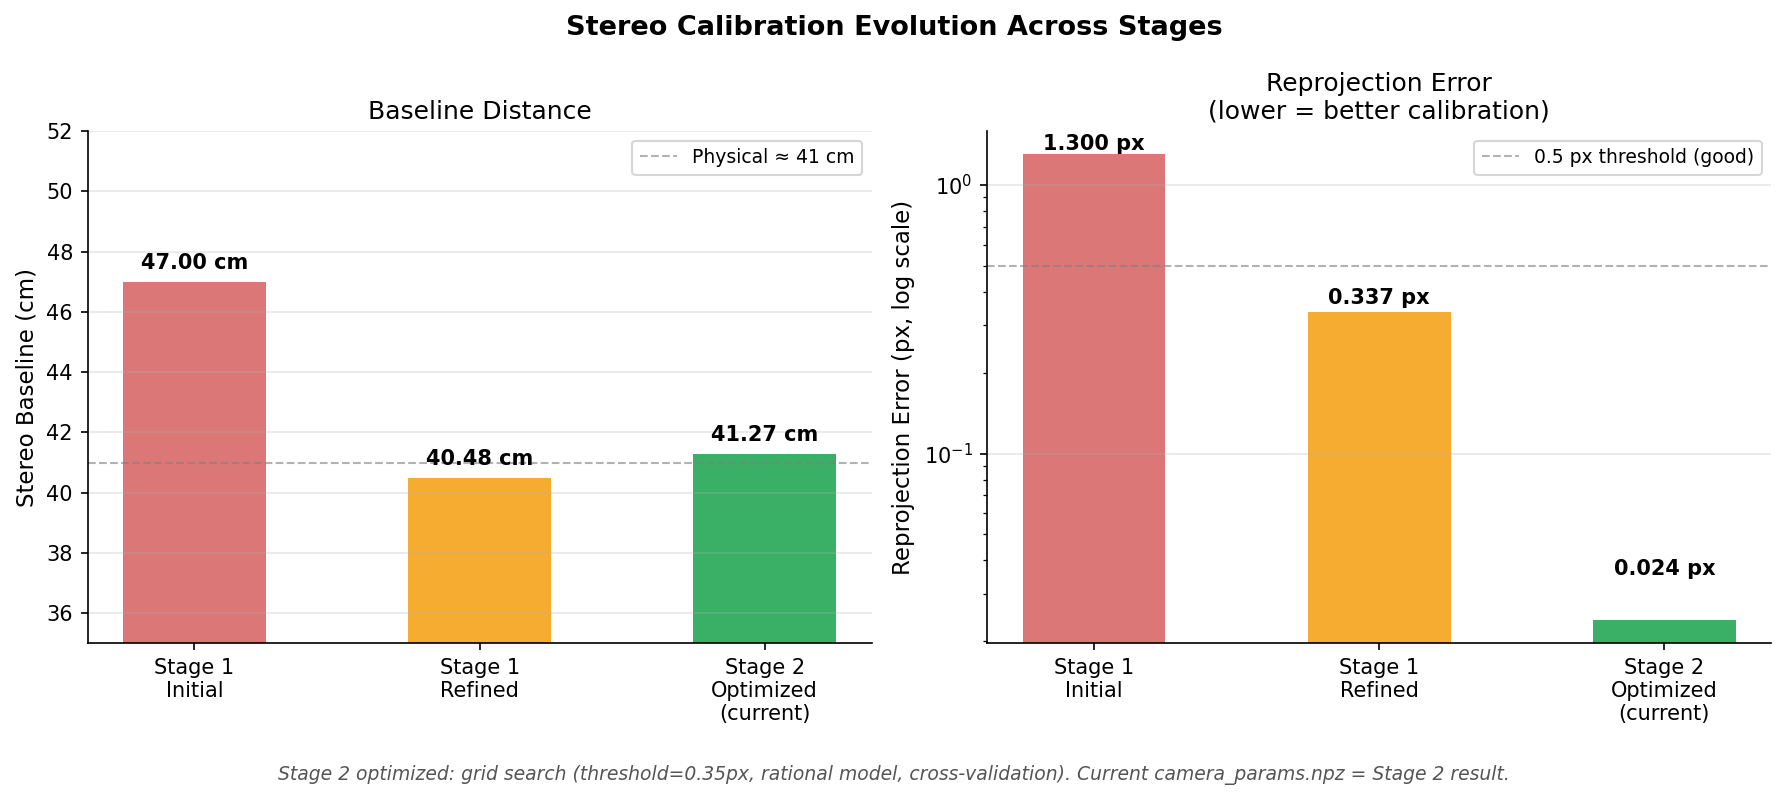
\includegraphics[width=\linewidth]{calibration_evolution.png}
  \caption{Stereo calibration evolution. The current calibration balances a realistic baseline estimate with a low reprojection error, making it suitable as the fixed geometric input for SKT.}
  \label{fig:calibration_evolution}
\end{figure}

\subsection{2025 Ergonomics Dataset}

All quantitative results in this thesis are computed on a single
single-subject ergonomics recording collected in a controlled
manufacturing-like environment, and this is therefore the dominant
generalisability limitation of the present study.
The subject performs a representative mix of factory-floor activities --
walking, sitting, squatting, reaching, lifting, and interacting with
furniture -- so that all major upper- and lower-body postures are exercised
within a single contiguous take rather than as isolated short clips.
After left--right pairing by hardware frame identifier, the usable
synchronised camera timeline contains 2801 frame pairs spanning 248.8\,s,
which corresponds to an effective frame rate of 12.5\,fps; the left raw
metadata contains 3015 rows and the right raw metadata contains 2882 rows,
so a non-trivial fraction of each side is either unpaired or falls outside
the synchronised interval, which is exactly what motivates the explicit
hardware-ID re-pairing step rather than reliance on raw row indices.
Table~\ref{tab:timeline_summary} summarises the resulting working timeline
that all downstream evaluations share.

\begin{table}[!htbp]
  \centering
  \caption{Summary of the synchronized camera timeline used for evaluation.}
  \label{tab:timeline_summary}
  \begin{tabular}{lc}
    \toprule
    Quantity & Value \\
    \midrule
    Synchronized frame pairs & 2801 \\
    Duration & 248.8 s \\
    Median frame interval & 0.0800 s \\
    Effective frame rate & 12.50 fps \\
    Left metadata rows & 3015 \\
    Right metadata rows & 2882 \\
    Rotation applied & 180\degr \\
    \bottomrule
  \end{tabular}
\end{table}

\subsection{Xsens Reference Data and Angle Representations}

The Xsens recording supplies full-body motion data on an independent time
axis and contains two distinct angle representations that the thesis must
choose between before any cross-method comparison can be reported.
The first is the \emph{Xsens native} joint-angle output, which is read
directly from the MVNX joint-angle channels and follows the Xsens body
model together with its internal axis and zero conventions.
The second is the \emph{Xsens-derived geometric} angle representation, in
which the joint angles are re-computed from the Xsens 3D segment positions
using the same three-point arccosine formula that is later applied to the
vision pipelines; this representation is adopted as the main reference
throughout the thesis because it removes the angle-definition mismatch
between the reference and the vision methods at the cost of being a
slightly less direct read of the Xsens body model.

The comparison between the two Xsens representations is then re-used as a
quantitative reference-system sanity check rather than discarded.
At the elbow, the two representations agree to within approximately
1--1.5\degr\ MAE in absolute angle space, and they agree to a Pearson
correlation of $\sim$0.99 in K-frame motion space; at the shoulder and hip,
the agreement is visibly weaker because the underlying axis conventions
differ more.
The implication for the thesis evaluation design is two-fold.
First, the elbow numbers serve as a \emph{lower-bound anchor}: a vision
method whose absolute angle MAE against Xsens-derived geometric is several
times the elbow self-consistency floor is unlikely to be limited by the
reference, whereas one that approaches the floor is approaching the
information limit of the reference itself.
Second, the larger shoulder/hip mismatch is one of the reasons the thesis
reports motion-space metrics alongside absolute angle MAE, since
differencing cancels both the unknown global Xsens calibration offset and
much of the axis-definition mismatch between the two representations.

\subsection{Cross-system Time Synchronisation}

Cross-system synchronisation is unavoidable for the present setup because
the cameras and the Xsens suit run on independent clocks, and any
mis-alignment converts directly into degraded motion-space agreement, so
the thesis adopts an automatic three-score offset search rather than a
manually picked shift.
The procedure first sweeps the offset coarsely between 0 and 30\,s, then
refines around the best candidate; at every candidate it computes three
independent agreement scores -- a position-space score on the 3D segment
positions, an angle-space score on the joint angles, and a motion-delta
score on the K-frame angle deltas -- and selects the motion-delta optimum
as the final offset because the motion evaluation is the most sensitive of
the three to residual sub-second mis-alignment.

For the present recording, the selected offset is 17.31\,s, and the
position-, angle-, and motion-delta optima fall at 17.27\,s, 17.28\,s, and
17.31\,s respectively.
The fact that three scores derived from three independent error spaces
converge inside a window of about 0.04\,s is the strongest evidence
available in this thesis that a single constant offset is an adequate
alignment model for this recording: had the underlying clock relation been
non-constant, the three scores would not be expected to peak so close
together.
Figure~\ref{fig:offset_search} shows the score curves produced by the
search and visualises this triple agreement.

\begin{figure}[!htbp]
  \centering
  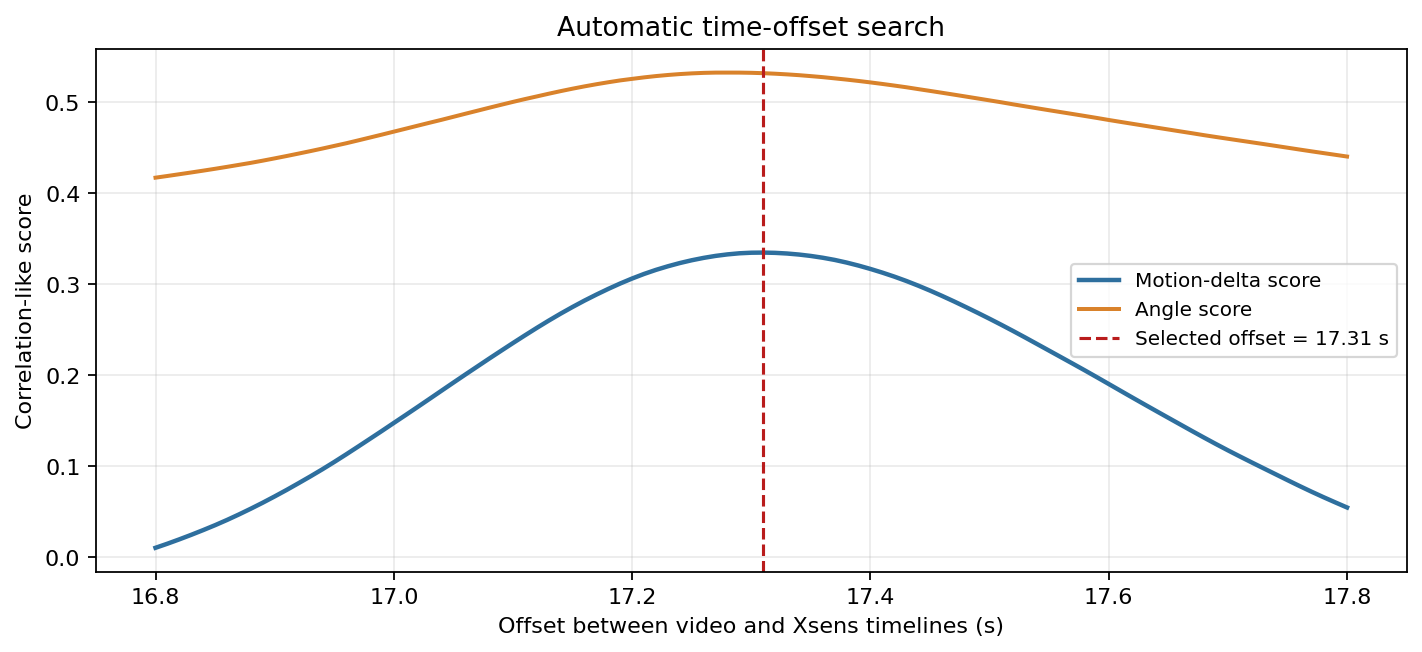
\includegraphics[width=\linewidth]{thesis_offset_search.png}
  \caption{Automatic offset estimation between the camera timeline and the Xsens reference timeline. The final selected value is 17.31 s, with position-, angle-, and motion-based scores all supporting a similar alignment.}
  \label{fig:offset_search}
\end{figure}

A second, qualitative synchronisation check is provided by overlaying the
aligned elbow-angle curves from all systems on the shared timeline
(Figure~\ref{fig:angle_time_alignment}).
The purpose of this plot is not to rank methods at the angle level -- that
is the task of Section~\ref{sec:results} -- but to confirm that the main
movement phases of the recording line up across systems after the offset
has been applied, so that any residual short-term deviation can be
attributed to true method behaviour rather than to an unfixed global shift.

\begin{figure}[!htbp]
  \centering
  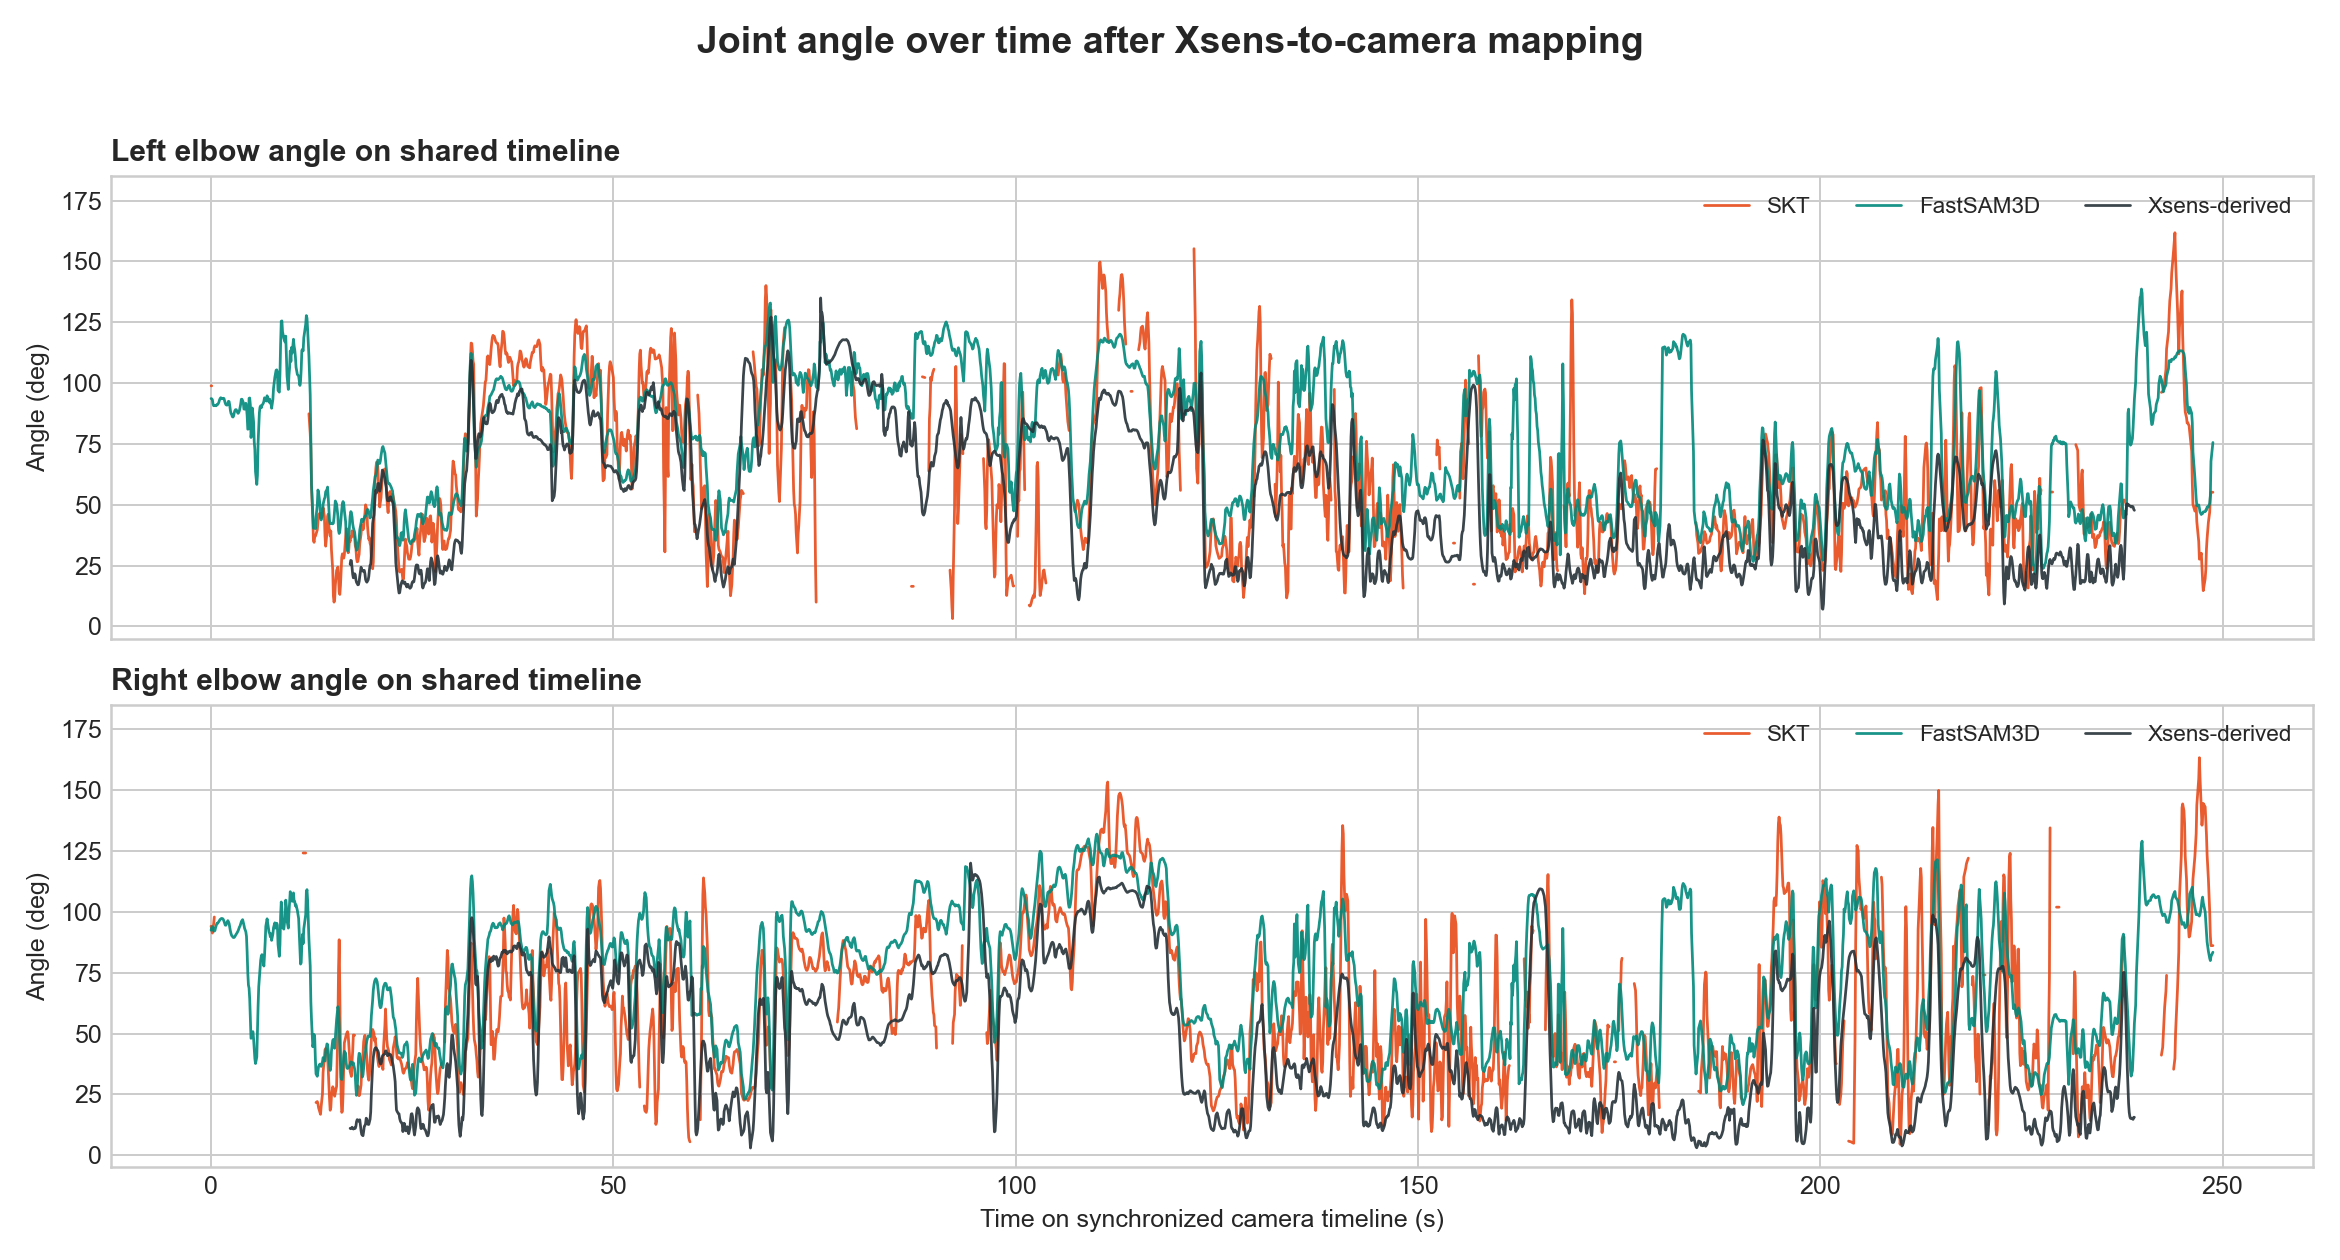
\includegraphics[width=\linewidth]{thesis_joint_angle_over_time.png}
  \caption{Left and right elbow angles on the shared timeline after offset correction. The plot provides a qualitative synchronisation check before quantitative angle and motion metrics are interpreted.}
  \label{fig:angle_time_alignment}
\end{figure}

A third check addresses the possibility that, even with a near-perfect
mean offset, the camera and Xsens clocks could drift slowly over the
$\sim$4\,min recording.
Figure~\ref{fig:first_last_delta} compares the K=6 motion-delta windows at
the beginning and end of the common valid interval; had the underlying
drift been large, the late-interval deltas would be expected to lose their
alignment with the reference even though the early-interval deltas still
agree.
The check is qualitative rather than a formal drift estimate, but the
observed late-interval agreement is comparable to the early-interval
agreement, which supports the use of a single constant offset for the
remainder of the thesis while explicitly acknowledging that future longer
or multi-take recordings should repeat this check.

\begin{figure}[!htbp]
  \centering
  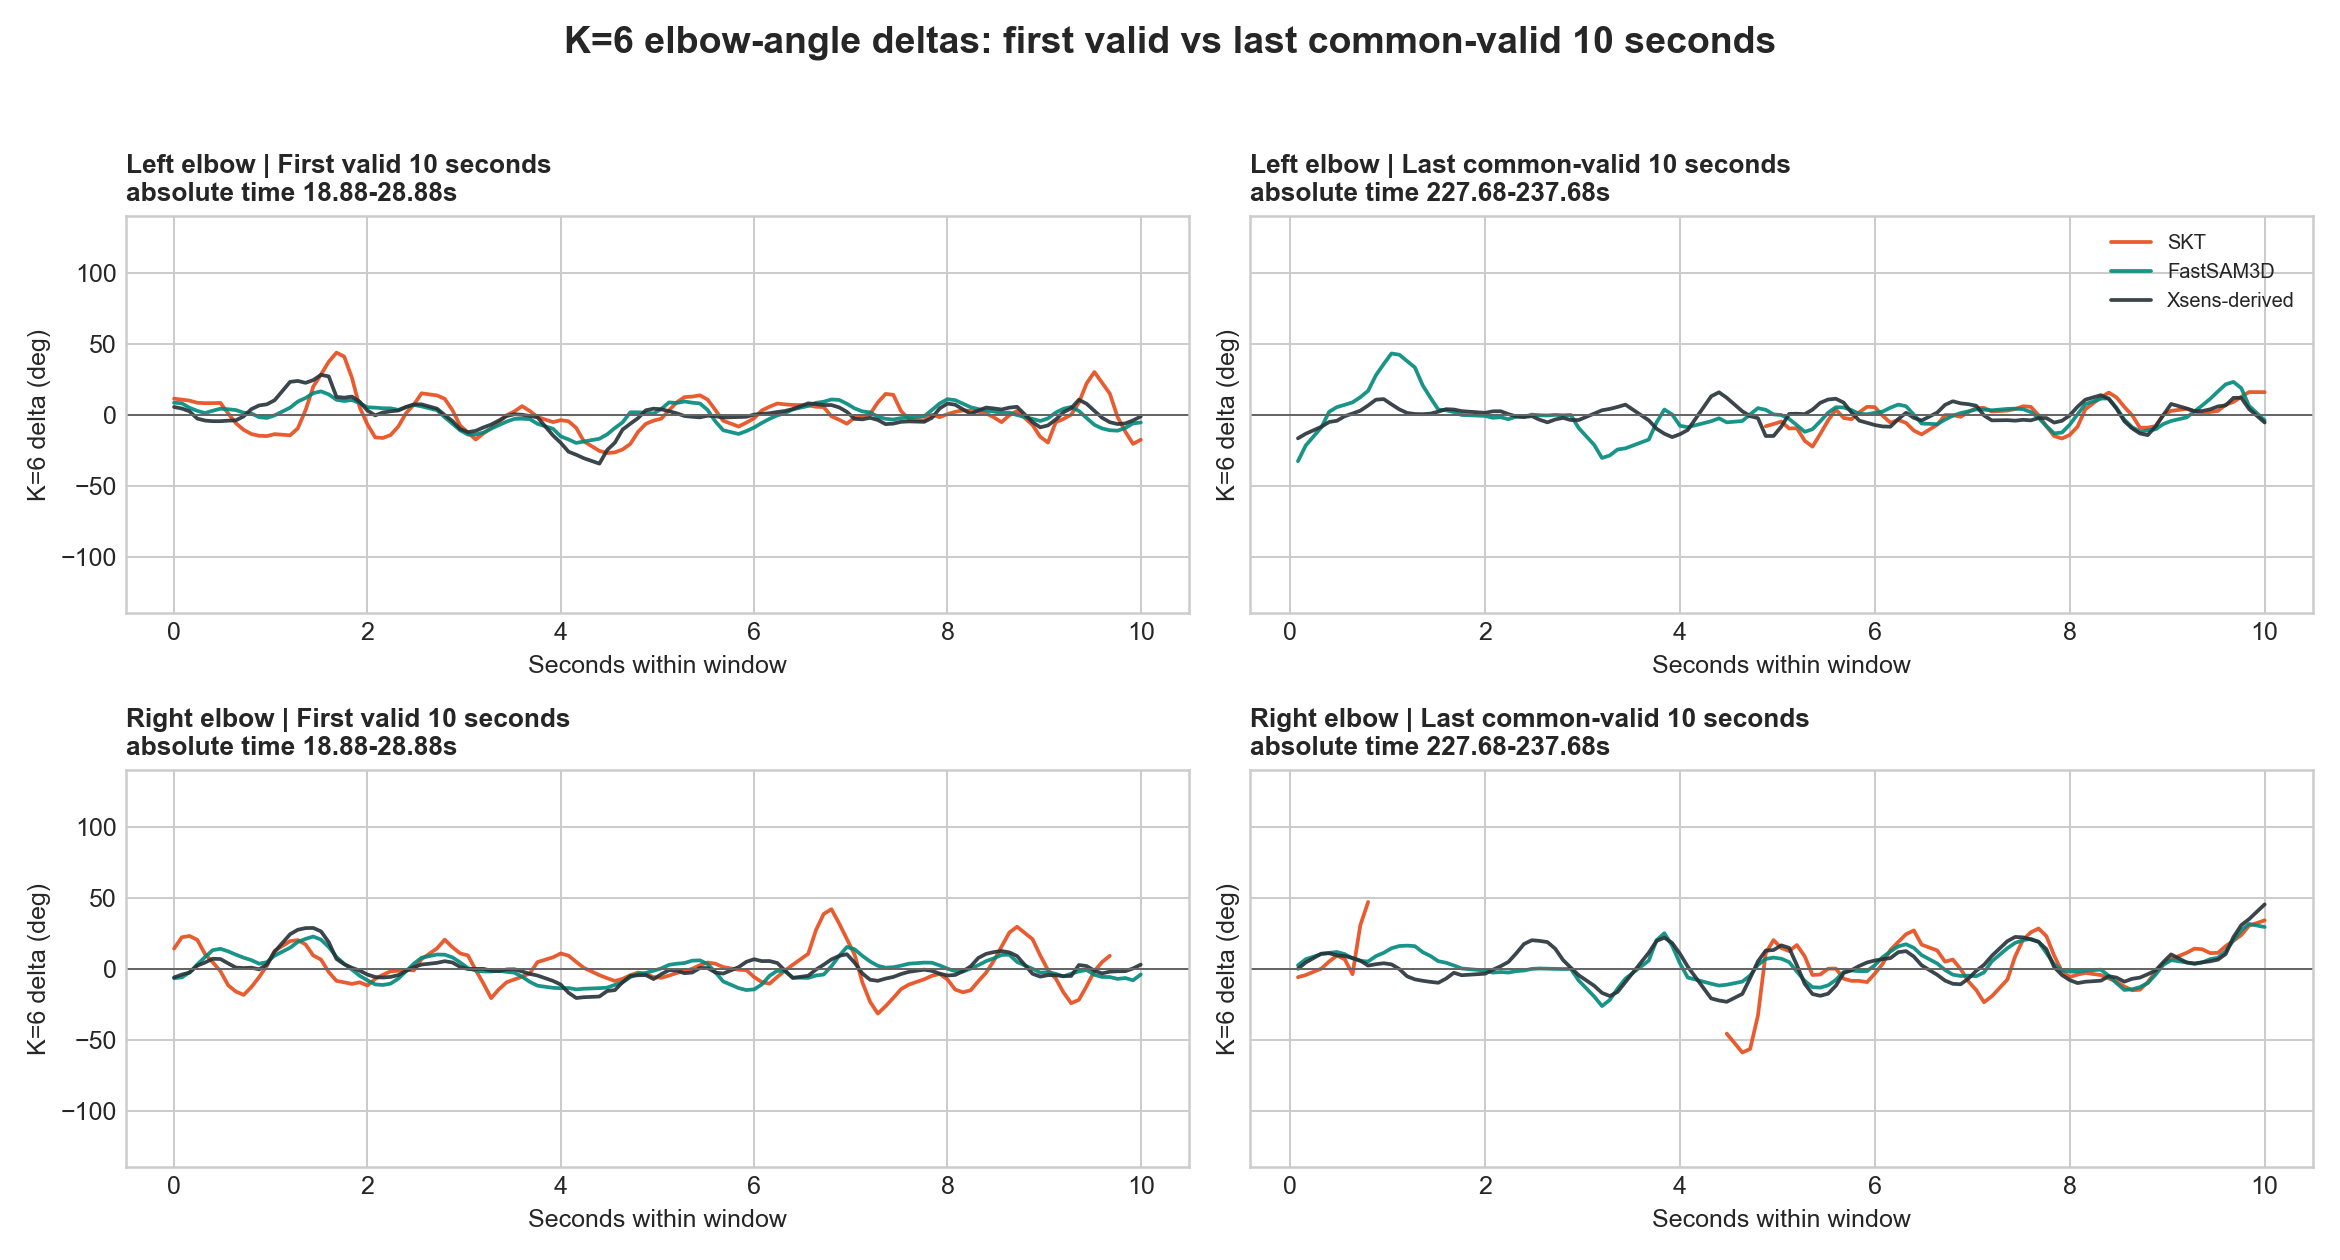
\includegraphics[width=\linewidth]{thesis_k6_delta_first_last_10s.png}
  \caption{K=6 elbow motion deltas near the beginning and end of the common valid interval. This figure is used as a practical check that the chosen constant offset remains reasonable across the recording.}
  \label{fig:first_last_delta}
\end{figure}

\clearpage
% =============================================================
\section{Methods}
\label{sec:methods}
% =============================================================

\subsection{Overview}

The thesis benchmarks two pose-estimation pipelines against the same Xsens
reference and the same evaluation protocol: SKT, the primary calibrated
sparse-stereo method developed in this thesis, and FastSAM3D, the monocular
learning-based alternative.
Figure~\ref{fig:pipeline_overview} shows the full experimental flow, and
Table~\ref{tab:method_roles} summarises each pipeline's input assumption, main
advantage, and main risk.

The single design choice that matters most for interpreting the rest of the
thesis is the deliberate separation between pose estimation and evaluation.
Both methods are mapped onto the same shared timeline and judged with
the same metrics, but those metrics are then split across two independent
axes (angle, motion) rather than collapsed into a single ranking
score; this prevents the recurring failure mode in which a method that is
strong in one space, for example metric stereo geometry, is implicitly
assumed to be equally strong in temporal angle consistency.

\begin{figure}[!htbp]
  \centering
  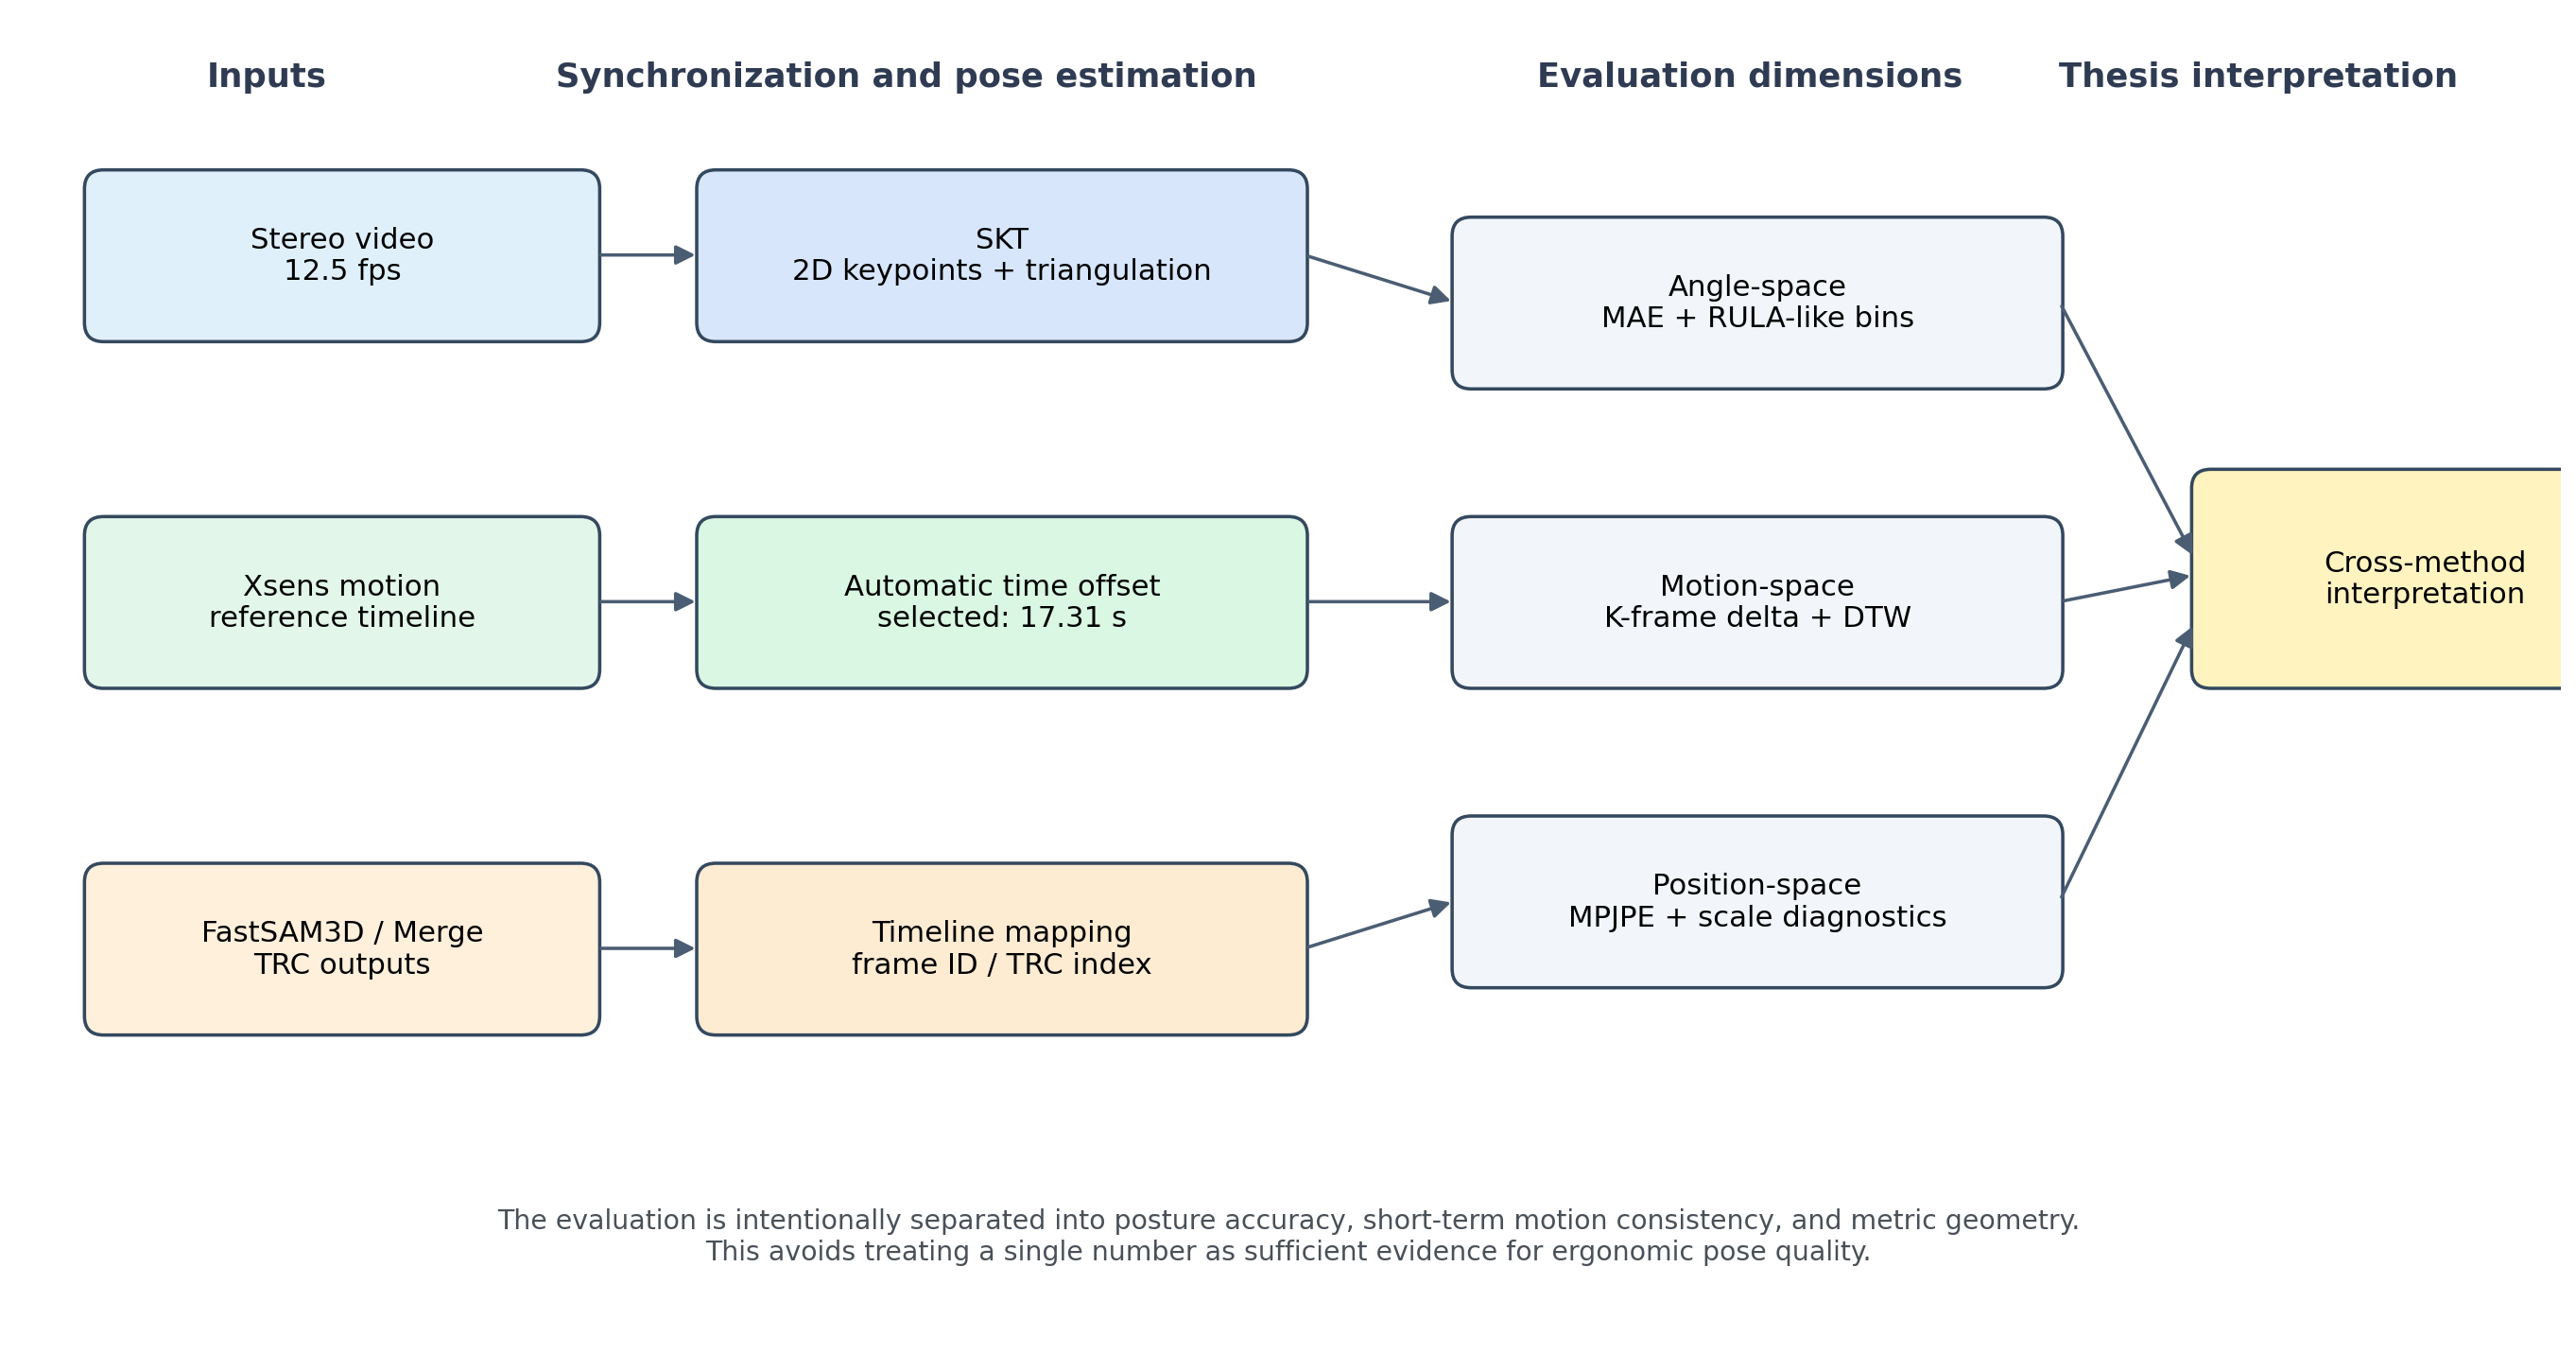
\includegraphics[width=\linewidth]{thesis_pipeline_overview.png}
  \caption{Overview of the thesis evaluation pipeline. Inputs are synchronized and evaluated separately in angle space, motion space, and position space before the final cross-method interpretation.}
  \label{fig:pipeline_overview}
\end{figure}

\begin{table}[!htbp]
  \centering
  \caption{Role of each evaluated pose-estimation path in the thesis.}
  \label{tab:method_roles}
  \small
  \begin{tabularx}{\linewidth}{lXXX}
    \toprule
    Method & Input assumption & Main advantage & Main risk \\
    \midrule
    SKT
    & Synchronized stereo video and calibrated cameras
    & Metric 3D scale and explicit geometric quality signals
    & 2D keypoint jitter and left--right mismatch are amplified by triangulation \\
    FastSAM3D
    & Monocular pose output provided as TRC markers
    & Learned body/motion priors give stable angle and motion behaviour
    & Coordinate, scale, and keypoint semantics require careful interpretation \\
    \bottomrule
  \end{tabularx}
\end{table}

\subsection{Sparse Keypoint Triangulation (SKT)}

The primary method developed in this thesis, Sparse Keypoint Triangulation
(SKT), turns a calibrated stereo video pair into a 3D body skeleton through
a transparent geometric chain that exposes per-frame quality signals at
every stage.
For each synchronised left/right frame pair, the pipeline first runs a 2D
human pose detector on each view to obtain 17 COCO-format keypoints with
per-keypoint confidence; the two views' keypoints are then matched by
keypoint index and filtered by three geometric consistency checks
(minimum triangulation confidence, maximum epipolar error, maximum
reprojection error after triangulation); the surviving pairs are
triangulated into 3D coordinates through the Direct Linear Transform
applied to the calibrated projection matrices; and finally the joint
angles are computed from triplets of 3D keypoints using the same
three-point arccosine formula that is applied to the Xsens-derived
geometric reference.

The methodological reason for building SKT this way -- rather than, for
example, regressing 3D pose directly with a learned model -- is
interpretability under deployment.
Every 3D point in an SKT output is tied to two observed 2D detections and
to a known stereo calibration model, so the pipeline can expose a set of
geometry-aware quality signals (triangulation confidence, epipolar error,
reprojection error, disparity) that downstream ergonomic monitoring can
use as a per-frame trust score; unreliable frames can therefore be
detected and gated rather than silently converted into ergonomic risk
scores, which is a property no end-to-end learned regressor offers for
free.
The corresponding methodological cost is that each SKT 3D point inherits
the noise of its 2D detections in both views; small 2D jitter is first
amplified by triangulation and then further amplified by joint-angle
computation, so SKT is most usefully understood as a measurement pipeline
whose output should be read together with its quality signals rather than
as a smoothed motion sequence.

This view of SKT as a measurement pipeline -- rather than a black-box
reconstruction module -- is also what motivates the later motion-delta
evaluation.
When a wrist or elbow keypoint is detected inconsistently between the two
views, the resulting 3D joint can remain numerically valid (the rays still
intersect, the reprojection is still small) while producing a sharply
different triangulated angle from the surrounding frames, which appears in
later analysis as occasional large motion deltas concentrated near
elbow-chain instabilities.
Section~\ref{sec:discussion} returns to these high-delta cases as concrete
failure evidence rather than treating them as generic noise.

\subsection{FastSAM3D (Monocular Learning Baseline)}

FastSAM3D is included as the learning-based monocular counterpart to SKT
and is the most informative single comparison in the thesis, because it
keeps the same input modality (the camera) but replaces multi-view
geometry with learned body-shape and motion priors.
Instead of triangulating left/right keypoint pairs, FastSAM3D produces a
3D pose directly from one camera stream through a model-based pipeline
that combines fast instance segmentation with learned body-shape and pose
priors \cite{yang2026fastsam3d}; the specific FastSAM3D
implementation is treated here as an externally produced output, and its
results are delivered as TRC marker files that are re-mapped to the
COCO-17 keypoint convention and resampled onto the shared camera timeline
before any evaluation metric is computed.

The methodological reason to include FastSAM3D is that learned body-shape
and motion priors should, in principle, smooth out the per-frame keypoint
noise that hurts SKT, because the learned model implicitly enforces
anatomically consistent transitions between consecutive poses even without
explicit multi-view evidence.
The corresponding methodological cost is that the FastSAM3D output does
not necessarily share the SKT coordinate frame, scale convention, or
exact keypoint semantics; FastSAM3D is therefore evaluated primarily in
the angle and motion axes, where these conventions cancel, while
position-space results are reported only as coordinate/scale diagnostics
rather than as direct pose-quality scores.

\clearpage
% =============================================================
\section{Evaluation Framework}
\label{sec:evaluation}
% =============================================================

\subsection{Angle-space Evaluation}

The angle-space track answers the most direct question for ergonomic
deployment -- ``Is the estimated joint posture quantitatively close to
the reference?'' -- and it is therefore reported first in every per-method
analysis even though it is the axis most exposed to the Xsens calibration
limitation discussed in Section~\ref{sec:background}.
Eight full-body angles are evaluated, covering the four bilateral joints
that drive most of the RULA assessment: left and right shoulder, elbow,
hip, and knee flexion.
To remove angle-definition mismatch between systems, every angle is
computed from the same three-point geometric formula applied to the
relevant triplet of 3D keypoints, both for the vision methods and for the
Xsens-derived geometric reference:
\begin{equation}
  \theta = \arccos\!\left(
    \frac{(\mathbf{p}_A-\mathbf{p}_B)\cdot(\mathbf{p}_C-\mathbf{p}_B)}
         {\|\mathbf{p}_A-\mathbf{p}_B\|\;\|\mathbf{p}_C-\mathbf{p}_B\|}
  \right).
\end{equation}
The main reported metrics are mean absolute error (MAE), median absolute
error, bias (signed mean error), valid-pair ratio, and -- as the
application-level companion -- RULA-like bin agreement for the
upper-body joints.

\subsection{Motion-space Evaluation}

The motion-space track is the thesis's principal countermeasure against
the Xsens calibration offset: it asks whether two systems describe the
\emph{same change in posture} rather than the same absolute posture, so
that any static reference offset cancels out by differencing.
For a given time scale $K$, the K-frame angle delta is defined as
\begin{equation}
  \Delta_K \theta_t \;=\; \theta_t \;-\; \theta_{t-K},
\end{equation}
and the thesis evaluates four time scales, $K\in\{1,6,12,25\}$ frames
(approximately 0.08, 0.48, 0.96, and 2.00\,s at 12.5\,fps), to probe the
agreement across genuinely instantaneous changes, sub-second sub-actions,
1\,s smooth-motion windows, and 2\,s near-action-level windows.
K=6 is adopted as the main reporting and visualisation scale because it
corresponds to a $\sim$0.48\,s sub-action -- short enough to remain a
true motion-level metric, long enough to suppress per-frame keypoint
jitter -- while the K=1 and K=25 numbers provide context as the
noise-dominated and amplitude-dominated extremes.
Reported metrics include Pearson correlation, Spearman rank correlation,
delta MAE and RMSE, high-delta count, and the path ratio (cumulative
absolute target delta divided by cumulative absolute reference delta),
which together separate ``shape agreement'' from ``amplitude agreement''
in the motion signal.

\subsection{Segment-level Evaluation}

The segment-level track condenses the frame-level motion comparison into
a small set of physically interpretable active-movement intervals,
because reporting only frame-level metrics tends to hide whether a method
captures the actual movement bursts that ergonomic risk assessment cares
about.
Activity segments are detected from the reference signal as contiguous
intervals of sustained K-frame motion above a threshold, and for each
segment four numbers are reported per method: range of motion (ROM,
max-min angle), per-segment angle MAE, RULA-like bin agreement based on
the segment's peak angle, and a dynamic time warping (DTW) distance
\cite{sakoe1978dtw}.
The DTW comparison is run on \emph{mean-subtracted and L2-normalised}
per-segment angle sequences, following the practice that has been
recommended for human-motion shape comparison in the recent literature
\cite{perezluque2026reaching}; the normalisation deliberately removes
absolute offset and amplitude so that DTW measures whether the
\emph{shape of motion through the segment} is similar, making it
complementary to MAE/RMSE (which measure amplitude error) rather than
redundant with them.

\subsection{Position-space Evaluation}

The position-space track does not compete with the angle and motion
tracks for ``best pose method'' -- it answers a separate deployment
question: ``Which method produces 3D coordinates whose scale and
geometry can be trusted in a metric workspace?''
For SKT, calibrated stereo geometry gives the coordinates an inherent
metric scale, so MPJPE-style distances and pelvis-relative comparisons
can be reported directly after rigid alignment using the standard Kabsch
estimator \cite{kabsch1976solution}.
For FastSAM3D, the output coordinate frame and scale convention do not
necessarily match the stereo or Xsens frames, so position-space numbers
must be reported with explicit alignment provenance; the thesis uses
position-space results primarily to (i) demonstrate stereo's
metric-scale advantage and (ii) document the coordinate/scale work that
any monocular pipeline must do before its 3D output becomes deployable.

\subsection{Filtering Policy}

The evaluation tracks above are well-defined only if the per-system
filtering policy is itself controlled, because temporal smoothing
applied at different strengths to different systems can quietly inflate
or deflate motion-space agreement without changing any reported number
in an obvious way.
The thesis therefore adopts a deliberate per-system policy.
Xsens streams are interpolated onto the shared timeline but are
\emph{not} re-smoothed by the project, because the Xsens internal
processing already includes substantial filtering, and stacking a
project-side filter on top would silently double the smoothing on
the reference side of every comparison.
The camera-based methods are smoothed with a single light moving-average
filter whose window is recorded in the run configuration; the chosen
window represents a $\sim$200\,ms low-lag setting consistent with empirical
guidance for human upper-body motion signals \cite{perezluque2026reaching}.
The single methodological invariant that must hold across all runs is
that smoothing is always applied \emph{before} delta computation, since
the opposite order would let the delta metric measure filter artifacts
rather than the underlying motion signal.

\begin{table}[!htbp]
  \centering
  \caption{Interpretation of the evaluation tracks used in the thesis.}
  \label{tab:evaluation_tracks}
  \small
  \begin{tabularx}{\linewidth}{lXXX}
    \toprule
    Track & Question answered & Main metrics & Main caveat \\
    \midrule
    Angle-space
    & Is the posture suitable for ergonomic angle interpretation?
    & MAE, median AE, bias, valid ratio, RULA-like bin agreement
    & Sensitive to reference-system angle definitions and static offsets \\
    Motion-space
    & Do two systems describe the same short-term movement?
    & K-frame delta correlation, delta MAE, RMSE, high-delta count, DTW
    & Requires careful time alignment and consistent smoothing policy \\
    Segment-level
    & Are active movement intervals similar in range and shape?
    & ROM error, segment MAE, DTW distance, RULA-like agreement
    & Depends on segment detection thresholds and valid-frame coverage \\
    Position-space
    & Are reconstructed 3D skeletons geometrically compatible?
    & MPJPE, pelvis-relative distance, aligned inter-method distance
    & Monocular methods may use different coordinate and scale conventions \\
    \bottomrule
  \end{tabularx}
\end{table}

This separation is central to the thesis argument.
For example, a method can produce good angle trends while still being
difficult to compare in absolute 3D coordinates, or it can preserve metric
scale while producing jittery short-term angles.
The evaluation framework therefore reports multiple complementary quantities
instead of selecting a single ``winner'' metric.

\clearpage
% =============================================================
\section{Results}
\label{sec:results}
% =============================================================

\subsection{Angle-space Results}

In the angle-space track, the monocular learning-based FastSAM3D pipeline
outperforms SKT, but the margin is small enough that the result must be
read with the Xsens reference-system caveat in mind rather than as a
universal verdict.
Averaged across the eight evaluated joint angles, FastSAM3D reaches a mean
MAE of 15.4\degr\ against the Xsens-derived reference, compared with
17.6\degr\ for SKT; the corresponding median MAEs (14.4\degr\ vs.\
17.9\degr) preserve the same ranking, and FastSAM3D also has the higher
valid-pair ratio (0.905 vs.\ 0.746).
The Xsens-native check sits at 4.7\degr\ MAE, an order of magnitude below
the vision methods, and is reported in the same table only as a
reference-system internal anchor rather than as a competing pose method.

The most informative joint-level pattern is that the per-joint MAE
ranking is not flat across the eight angles.
Shoulder, hip, and knee angles dominate FastSAM3D's lead, where its
learned body priors stabilise the chain endpoints; the elbow is the
hardest joint for every vision method, in line with the long
shoulder--elbow--wrist chain that amplifies both keypoint noise (for SKT)
and pose-prior uncertainty (for FastSAM3D), and this is the joint where
both methods are penalised most by the Xsens calibration offset
itself.
For this reason the elbow is the joint that drives the motion-space
analysis that follows -- angle MAE alone cannot tell which fraction of
the elbow error is genuine pose error and which fraction is reference
offset.

\begin{table}[!htbp]
  \centering
  \caption{Angle-space summary across eight evaluated joint angles. Lower MAE is better.}
  \label{tab:angle_summary}
  \small
  \begin{tabular}{lcccc}
    \toprule
    Method & Mean MAE $\downarrow$ & Median MAE $\downarrow$ &
    Valid ratio $\uparrow$ & Bin agreement $\uparrow$ \\
    \midrule
    SKT & 17.6 & 17.9 & 0.746 & 0.540 \\
    \good{FastSAM3D} & \good{15.4} & \good{14.4} & \good{0.905} & \good{0.553} \\
    \textit{Xsens native check} & \textit{4.7} & \textit{3.7} & \textit{0.905} & \textit{0.886} \\
    \bottomrule
  \end{tabular}
\end{table}

Figure~\ref{fig:angle_summary_plot} visualises the same comparison.
The bar plot is included precisely because the FastSAM3D--SKT gap is
small and consistent rather than large and dramatic; a single bar
that was twice as high as another would not survive any reasonable
sensitivity check on this single recording, whereas a small but
systematic gap is the more honest evidence on which to base the
discussion of learned pose priors later in the thesis.

\begin{figure}[!htbp]
  \centering
  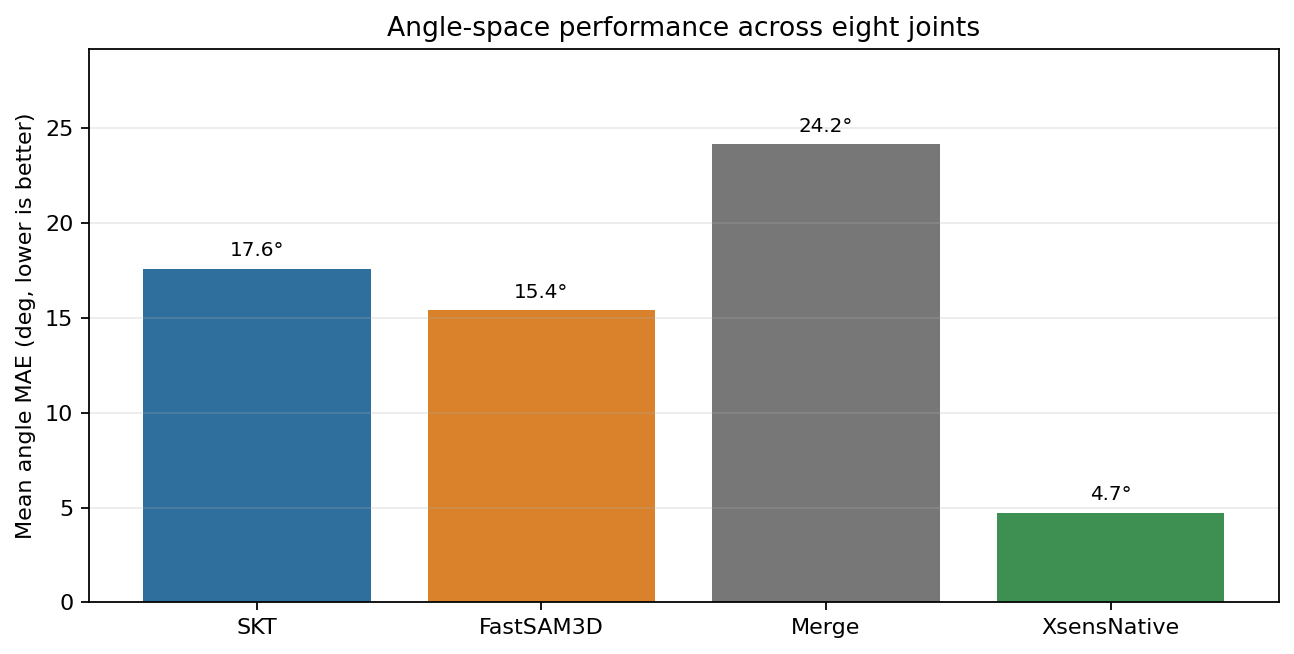
\includegraphics[width=0.92\linewidth]{thesis_angle_summary.png}
  \caption{Angle-space summary across evaluated methods. FastSAM3D has the lowest mean and median MAE among the vision methods, while the Xsens-native check indicates the approximate lower bound of the reference-system representation difference.}
  \label{fig:angle_summary_plot}
\end{figure}

\subsection{Motion-space Results}

In the motion-space track, the FastSAM3D advantage observed in absolute
angles becomes both clearer and easier to interpret, because differencing
the angle sequences cancels the Xsens calibration offset that confounded
the angle-space comparison.
Averaged across the eight evaluated angles at $K=6$ frames ($\sim$0.48\,s),
FastSAM3D reaches a mean Pearson correlation of 0.64 with the Xsens-derived
reference, against 0.38 for SKT; the corresponding mean Spearman rank
correlations (0.64 vs.\ 0.33) preserve the same ranking, which rules out
the explanation that FastSAM3D is winning only because of a handful of
high-amplitude points that inflate Pearson without lifting the rank
correlation.
At the elbow -- the joint that the motion-space track is designed to
adjudicate -- FastSAM3D reaches Pearson correlations of 0.54 (left) and
0.69 (right) against SKT's 0.39 / 0.39, a comparable shape-agreement gap
on the joint that the angle-space analysis flagged as ambiguous.
The Xsens-native check returns the expected $\sim$0.96 mean correlation,
confirming that the K=6 metric can recover near-perfect agreement when
the two compared signals genuinely measure the same motion.

\begin{table}[!htbp]
  \centering
  \caption{K=6 motion-delta agreement. Higher correlation is better.}
  \label{tab:motion_summary}
  \small
  \begin{tabular}{lcccc}
    \toprule
    Method & Mean $r$ $\uparrow$ & Mean $\rho$ $\uparrow$ &
    L-elbow $r$ $\uparrow$ & R-elbow $r$ $\uparrow$ \\
    \midrule
    SKT & 0.379 & 0.334 & 0.392 & 0.386 \\
    \good{FastSAM3D} & \good{0.644} & \good{0.635} & \good{0.542} & \good{0.689} \\
    \textit{Xsens native check} & \textit{0.965} & \textit{0.936} & \textit{0.988} & \textit{0.993} \\
    \bottomrule
  \end{tabular}
\end{table}

Figure~\ref{fig:motion_k6_summary_plot} visualises the K=6 correlation
summary and makes the main finding immediately legible: FastSAM3D is
consistently above SKT across the eight evaluated angles, and the Xsens-native
check provides the visual upper bound that anchors the scale of the plot.
The per-elbow scatter plots in Figure~\ref{fig:k6_elbow_scatter} then make
the same comparison at the frame level rather than the summary level:
FastSAM3D's scatter clusters along the ideal diagonal with limited vertical
spread, whereas SKT's scatter shows a recurring vertical accumulation near
zero reference delta -- the geometric signature of high SKT delta values
during physically quiet intervals, which Section~\ref{sec:discussion}
traces back to localised keypoint-chain instability rather than to a
constant noise floor.

\begin{figure}[!htbp]
  \centering
  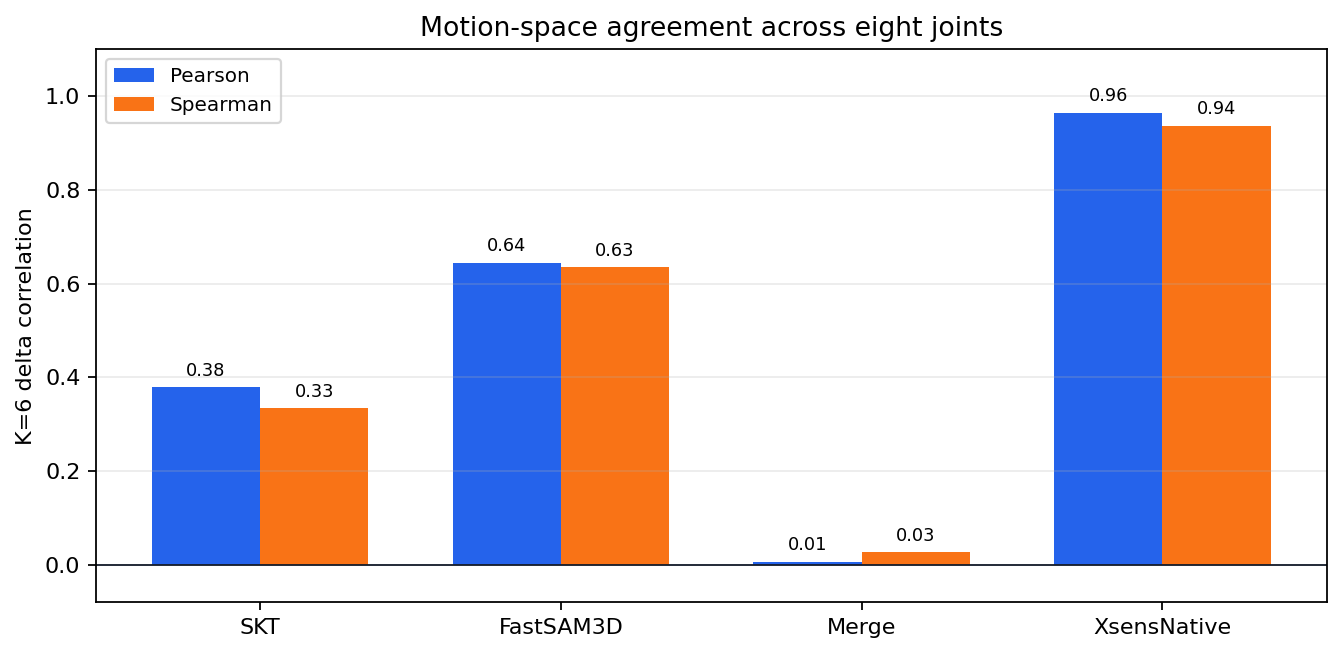
\includegraphics[width=0.92\linewidth]{thesis_motion_k6_summary.png}
  \caption{K=6 motion-delta correlation summary. FastSAM3D shows stronger short-term motion agreement than SKT on the current dataset.}
  \label{fig:motion_k6_summary_plot}
\end{figure}

\begin{figure}[!htbp]
  \centering
  \begin{subfigure}[b]{0.48\linewidth}
    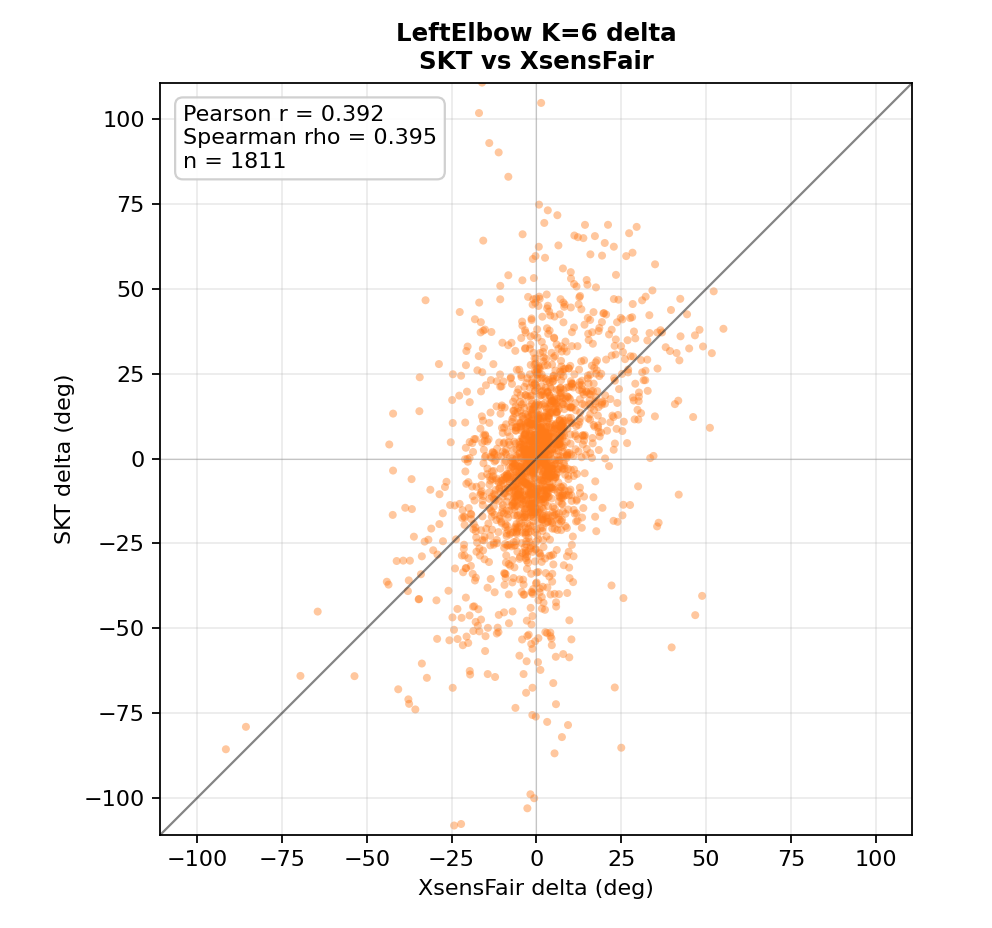
\includegraphics[width=\linewidth]{thesis_scatter_skt_vs_xsensfair_leftelbow_k6.png}
    \caption{SKT, left elbow.}
  \end{subfigure}
  \hfill
  \begin{subfigure}[b]{0.48\linewidth}
    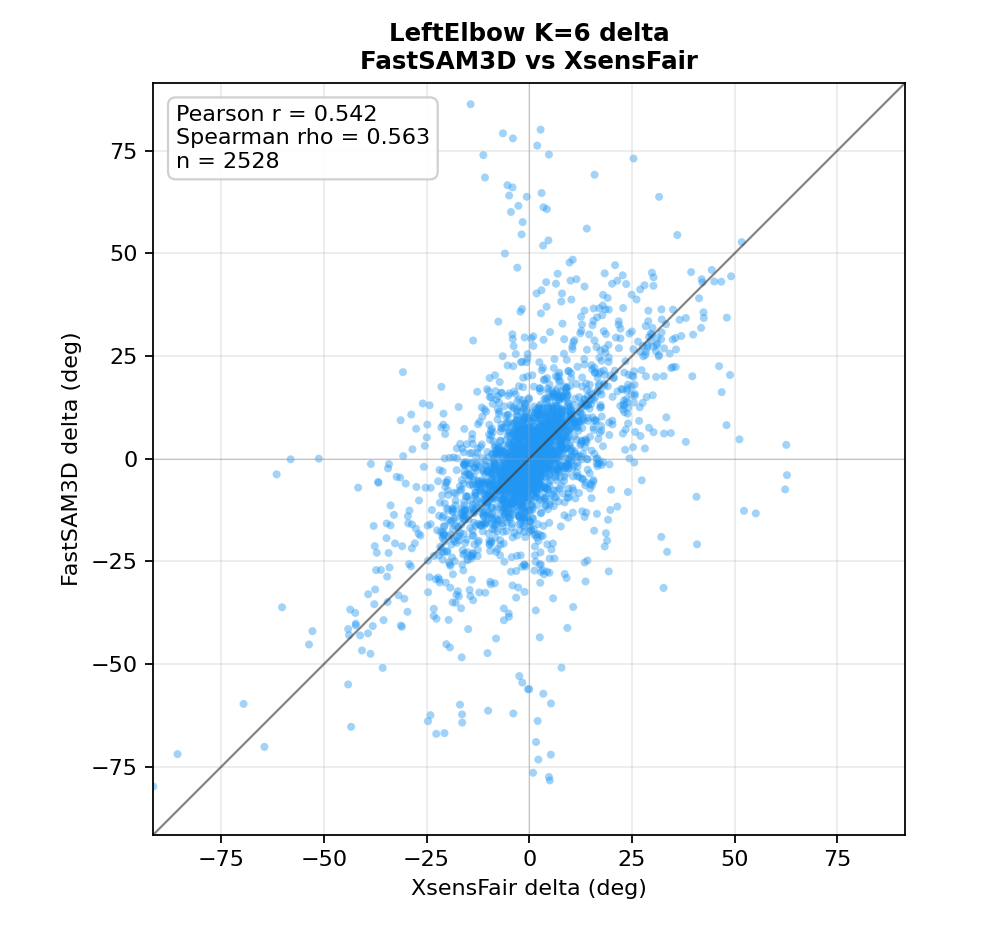
\includegraphics[width=\linewidth]{thesis_scatter_fastsam3d_vs_xsensfair_leftelbow_k6.png}
    \caption{FastSAM3D, left elbow.}
  \end{subfigure}

  \vspace{0.4cm}
  \begin{subfigure}[b]{0.48\linewidth}
    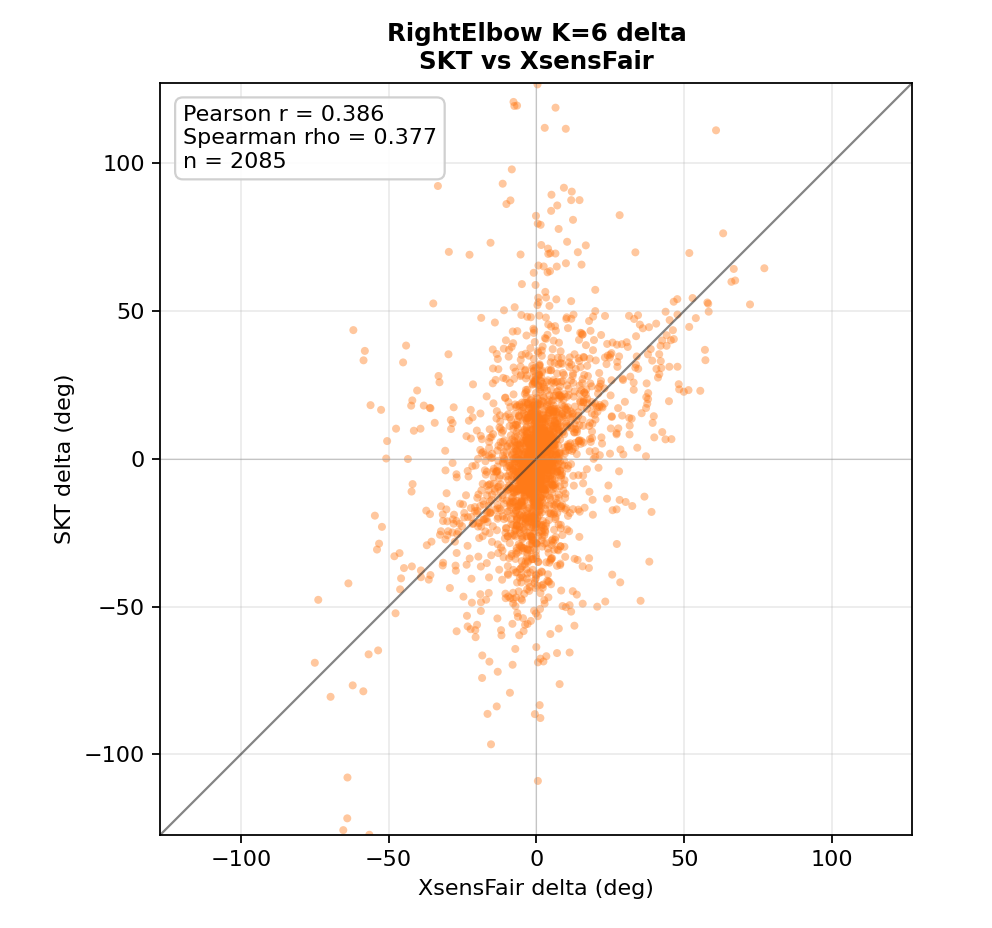
\includegraphics[width=\linewidth]{thesis_scatter_skt_vs_xsensfair_rightelbow_k6.png}
    \caption{SKT, right elbow.}
  \end{subfigure}
  \hfill
  \begin{subfigure}[b]{0.48\linewidth}
    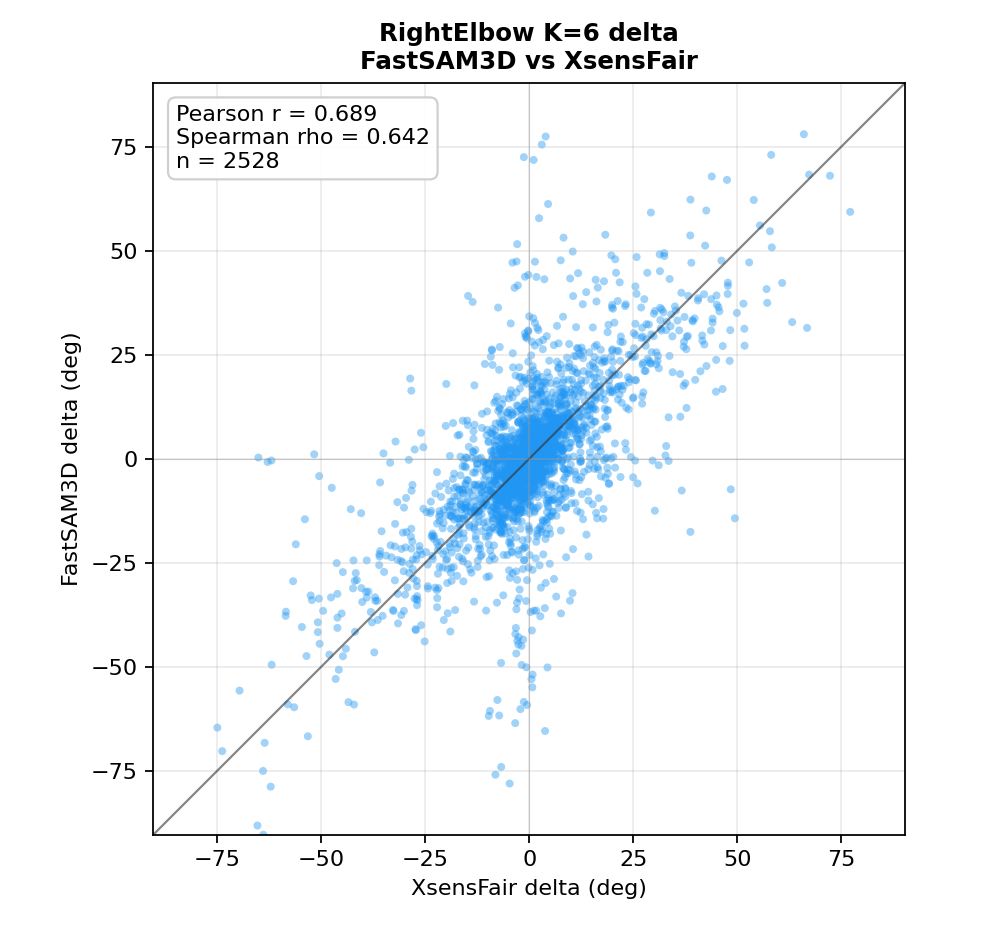
\includegraphics[width=\linewidth]{thesis_scatter_fastsam3d_vs_xsensfair_rightelbow_k6.png}
    \caption{FastSAM3D, right elbow.}
  \end{subfigure}
  \caption{K=6 elbow motion-delta scatter plots against the Xsens-derived reference. FastSAM3D follows the ideal trend more consistently, while SKT shows more high-delta jitter and vertical-axis accumulation.}
  \label{fig:k6_elbow_scatter}
\end{figure}

The sensitivity of the motion-space ranking to the chosen time scale is
shown in Figure~\ref{fig:pearson_vs_k}.
At $K=1$ (single-frame deltas, $\sim$80\,ms) every vision method's
correlation drops because the metric is dominated by per-frame keypoint
jitter that is roughly uncorrelated with the reference; at $K=25$
($\sim$2\,s) every vision method's correlation rises because the metric
is approaching an amplitude-of-motion comparison rather than a true
short-term agreement.
The thesis adopts $K=6$ as the main reporting point because it lies on
the elbow of these two trends: it suppresses single-frame keypoint noise
without smoothing across a complete action, so the ranking it produces
remains a genuine motion-agreement statement rather than either a
noise floor or a re-statement of segment-level ROM.

\begin{figure}[!htbp]
  \centering
  \begin{subfigure}[b]{0.48\linewidth}
    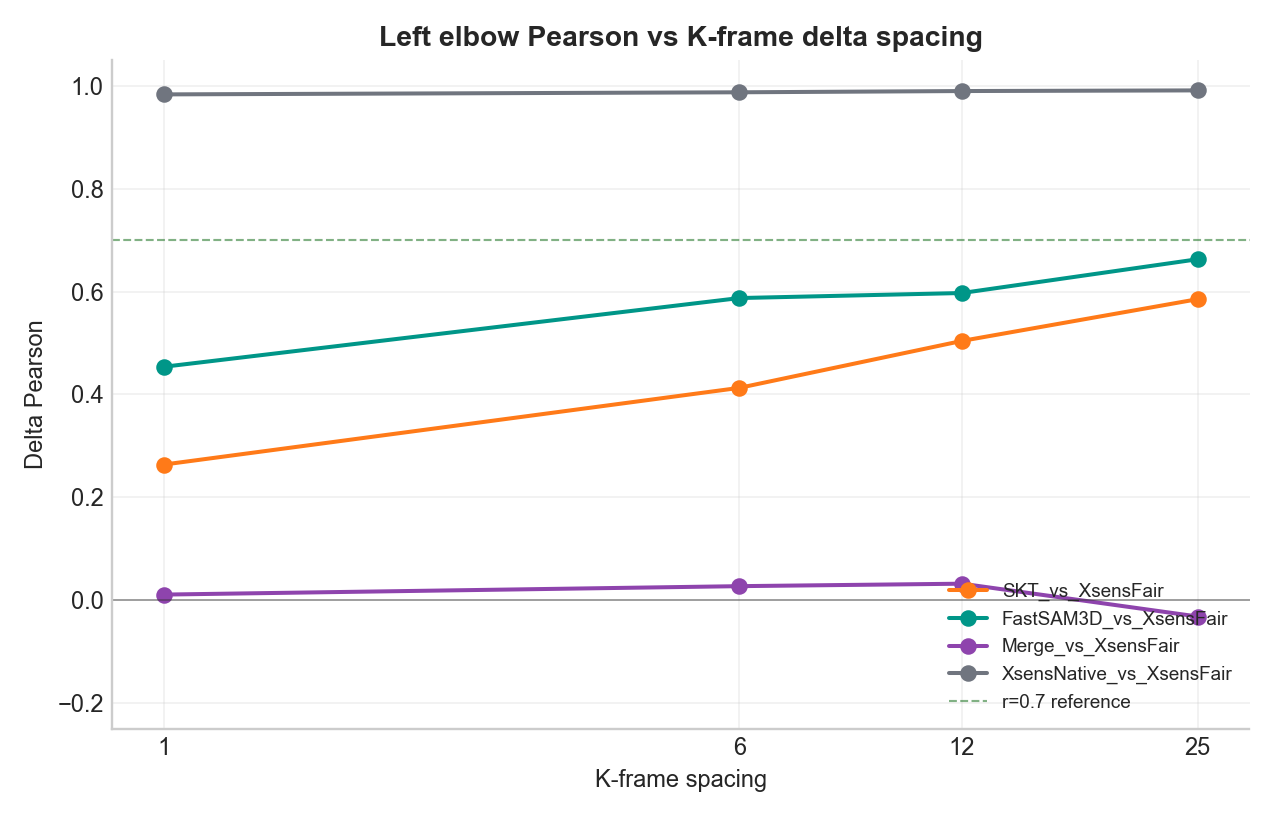
\includegraphics[width=\linewidth]{thesis_pearson_vs_k_leftelbow.png}
    \caption{Left elbow.}
  \end{subfigure}
  \hfill
  \begin{subfigure}[b]{0.48\linewidth}
    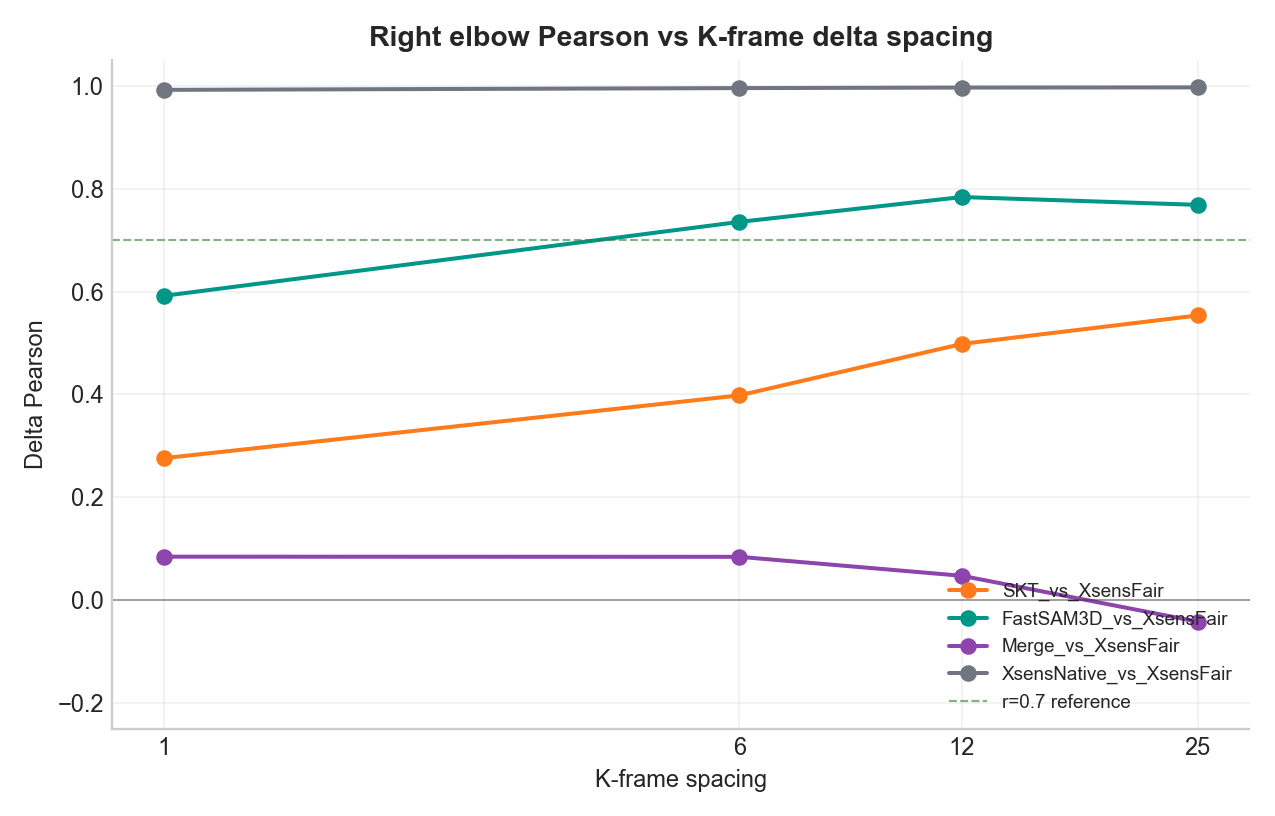
\includegraphics[width=\linewidth]{thesis_pearson_vs_k_rightelbow.png}
    \caption{Right elbow.}
  \end{subfigure}
  \caption{Motion-delta correlation as a function of K. The result supports using K=6 as a practical compromise between jitter sensitivity and motion interpretability.}
  \label{fig:pearson_vs_k}
\end{figure}

\subsection{Segment-level Results}

The segment-level track reinforces the frame-level motion finding while
adding two pieces of information that the frame-level numbers alone cannot
provide: per-segment range-of-motion (ROM) error in degrees, which is the
quantity most directly comparable to a ``movement size'' an ergonomist
would estimate manually, and per-segment normalised DTW distance, which
quantifies how similar the shape of motion through each segment is once
amplitude and offset are removed.
Aggregated over the detected active segments (39 for SKT, 45 for
FastSAM3D), FastSAM3D has both the lower mean ROM error (14.9\degr\ vs.\
26.9\degr\ for SKT) and the lower mean DTW distance (0.0355 vs.\ 0.0435).
The Xsens-native DTW distance ($\sim$6$\times 10^{-3}$) sets the lower
bound that the normalised DTW metric can reach on this dataset, so
FastSAM3D's $\sim$3.5$\times 10^{-2}$ is approximately six times the
reference floor, which is the right order of magnitude to claim
``competitive'' rather than ``saturated''.

\begin{table}[!htbp]
  \centering
  \caption{Segment-level summary over detected active movement intervals. Lower values are better.}
  \label{tab:segment_summary}
  \begin{tabular}{lccc}
    \toprule
    Method & Segments & Mean ROM error (\degr) $\downarrow$ & Mean DTW distance $\downarrow$ \\
    \midrule
    SKT & 39 & 26.9 & 0.0435 \\
    \good{FastSAM3D} & 45 & \good{14.9} & \good{0.0355} \\
    \textit{Xsens native check} & \textit{45} & \textit{4.8} & \textit{0.0062} \\
    \bottomrule
  \end{tabular}
\end{table}

\begin{figure}[!htbp]
  \centering
  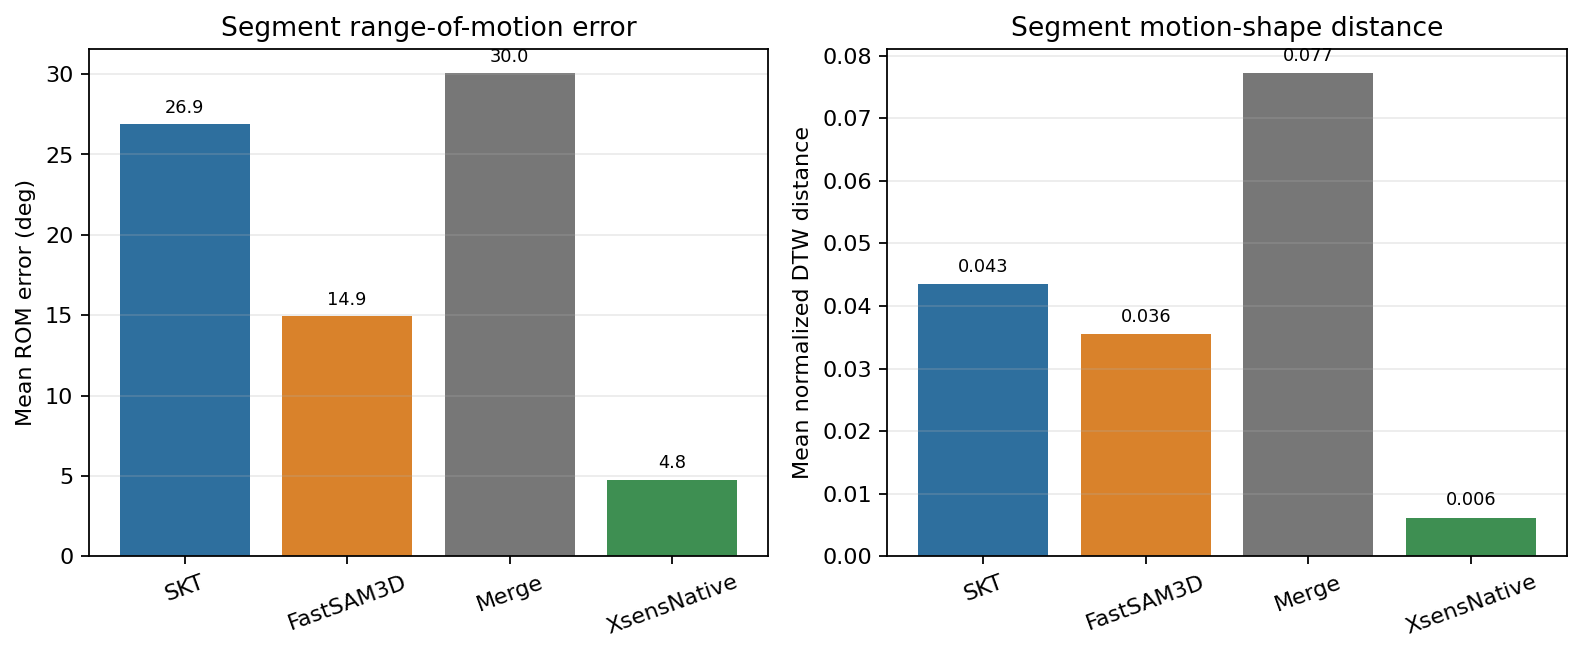
\includegraphics[width=0.95\linewidth]{thesis_segment_summary.png}
  \caption{Segment-level ROM error and DTW distance. FastSAM3D gives the strongest segment-level agreement among the vision methods, while the Xsens-native check provides a reference-system lower bound.}
  \label{fig:segment_summary_plot}
\end{figure}

\subsection{Position-space Results}

The position-space track produces a deliberately different interpretation
from the angle and motion tracks, and reading it as a competing
quality ranking would be a mistake.
SKT recovers 3D coordinates with metric scale inherited from calibrated
stereo geometry, so its distance to the Xsens-derived reference -- 30.6\,cm
mean (20.8\,cm median) after rigid Kabsch alignment -- is a meaningful
geometric quantity whose magnitude can be discussed in the same units as
the workspace itself.
FastSAM3D's direct distance to the Xsens reference under identical
coordinate assumptions is approximately 300\,cm, which is two orders of
magnitude larger; this number, however, does not say that FastSAM3D's
poses are visually two orders of magnitude worse -- it says that the raw
FastSAM3D output uses a different coordinate origin and scale convention,
and the dominant component of the 300\,cm distance is therefore a global
similarity transform that has not yet been resolved.
When FastSAM3D is instead aligned directly to SKT over a set of common
joints, the residual mean distance drops to approximately 60\,cm,
clarifying that the genuine inter-method 3D disagreement is at the
half-metre scale rather than the multi-metre scale and isolating it from
the coordinate-convention issue.

The methodological consequence is reported in
Table~\ref{tab:position_summary} rather than asserted in prose: the
position-space numbers must be read as \emph{coordinate/scale
diagnostics} that document the operational cost of using each method in
metric 3D space, not as another lap of the angle-space ranking
competition.
SKT inherits its metric scale automatically from the calibrated camera
baseline (Section~\ref{sec:data_setup}), so a downstream RULA scorer or
workspace-overlay tool can read its 3D coordinates directly; FastSAM3D
needs a separate scale/coordinate alignment step, which is feasible but
adds operational complexity that this thesis flags explicitly rather
than leaves implicit.

\begin{table}[!htbp]
  \centering
  \caption{Position-space diagnostic results. These values should be interpreted as coordinate/scale diagnostics rather than pure pose-quality rankings.}
  \label{tab:position_summary}
  \small
  \begin{tabularx}{\linewidth}{lccX}
    \toprule
    Comparison & Mean distance & Median distance & Notes \\
    \midrule
    SKT vs.\ reference & 30.6 cm & 20.8 cm & Metric stereo scale after rigid alignment \\
    FastSAM3D vs.\ reference & 300.3 cm & 294.8 cm & Coordinate/scale convention mismatch dominates \\
    FastSAM3D aligned to SKT & 60.0 cm & 36.3 cm & Direct inter-method skeleton comparison \\
    \bottomrule
  \end{tabularx}
\end{table}

\begin{figure}[!htbp]
  \centering
  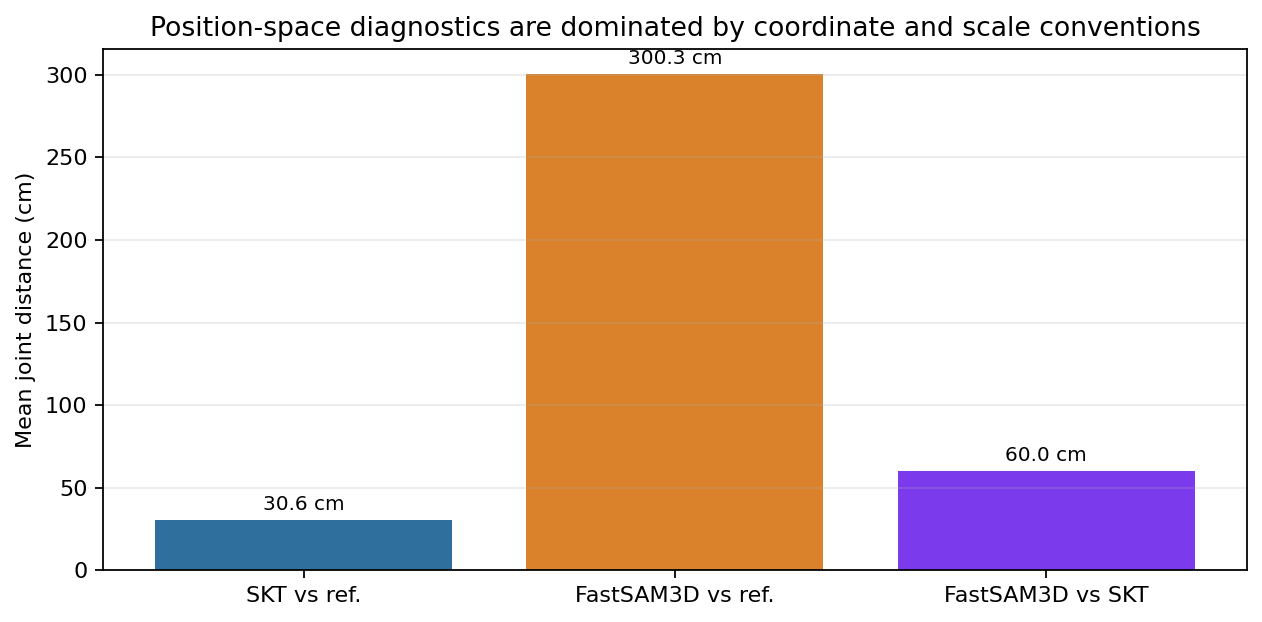
\includegraphics[width=0.9\linewidth]{thesis_position_diagnostic.png}
  \caption{Position-space diagnostic comparison. SKT is more meaningful in metric 3D space because it is tied to calibrated stereo geometry, whereas direct FastSAM3D-to-reference distance is dominated by coordinate and scale conventions.}
  \label{fig:position_diagnostic_plot}
\end{figure}

\subsection{Cross-method Synthesis}

Reading the two evaluation tracks together produces a more complete picture
than either gives on its own.
Table~\ref{tab:cross_method_synthesis} consolidates the headline numbers
for SKT and FastSAM3D (with the Xsens-native check shown alongside as a
reference-system floor).
FastSAM3D leads on the angle-space (lower MAE) and motion-space (higher
correlation) tracks, which together indicate that learned body and motion
priors suppress the per-frame jitter that hurts a frame-independent
sparse stereo reconstruction on this dataset.
SKT lags FastSAM3D on angle and motion but its 3D coordinates carry metric
scale by construction, and the per-frame geometric quality signals it exposes
(epipolar error, reprojection error, triangulation confidence) are exactly
the signals that downstream ergonomic quality gating requires.

\begin{table}[!htbp]
  \centering
  \caption{SKT vs FastSAM3D headline synthesis across evaluation tracks. Best value per column is highlighted; the Xsens-native row is a reference-system internal check, not a competing method.}
  \label{tab:cross_method_synthesis}
  \small
  \begin{tabular}{lccccl}
    \toprule
    Method & Angle MAE (\degr) $\downarrow$ & RULA bin agree.\ $\uparrow$ & Motion $r$ K=6 $\uparrow$ & Segment ROM (\degr) $\downarrow$ & Metric scale \\
    \midrule
    SKT
    & 17.6 & 0.540 & 0.379 & 26.9 & \good{Calibrated} \\
    \good{FastSAM3D}
    & \good{15.4} & \good{0.553} & \good{0.644} & \good{14.9} & Needs alignment \\
    \textit{Xsens native (ref.)}
    & \textit{4.7} & \textit{0.886} & \textit{0.965} & \textit{4.8} & \textit{---} \\
    \bottomrule
  \end{tabular}
\end{table}

The overall pattern is: \emph{the learning-based monocular pipeline wins
the angle and motion agreement tracks; the calibrated stereo pipeline
retains the deployment-geometry advantage; and neither replaces the other.}
This split is the substantive result of the synthesis and is what
Section~\ref{sec:discussion} examines in operational terms.

\clearpage
% =============================================================
\section{Discussion}
\label{sec:discussion}
% =============================================================

\subsection{Why FastSAM3D Performs Better in Angle and Motion Space}

The most likely reason FastSAM3D leads SKT on the angle and motion tracks
is that its learned body-structure and motion-continuity priors mask
exactly the per-frame failure mode that hurts a frame-independent
triangulation pipeline.
FastSAM3D's 3D output for any given frame is conditioned on body-shape
plausibility constraints that were absorbed from large pose-sequence
training corpora, so a momentarily unreliable keypoint produces a
smoothed-out anatomical correction rather than a sharp angle spike; this
is qualitatively visible in the K=6 elbow scatter plots
(Figure~\ref{fig:k6_elbow_scatter}), where the FastSAM3D scatter sits
along the ideal y=x diagonal whereas the SKT scatter shows recurring
vertical accumulation -- large target deltas at small reference deltas --
that no amount of point-density change can hide.
This shape of error matters for the interpretation: the SKT weakness is
not a uniform random noise floor but a structured failure pattern
concentrated on a small fraction of frames, which suggests that targeted
quality-aware repair rather than uniform smoothing is the appropriate
remedy.

\subsection{Why Stereo Geometry Still Matters}

The FastSAM3D advantage on the agreement tracks does not eliminate the
case for calibrated stereo geometry, because deployment in a real
manufacturing setting cares about two properties that the agreement
tracks alone do not test: whether the 3D coordinates are in real metric
units, and whether the system can flag its own unreliable frames before
they reach a downstream ergonomic risk score.
SKT inherits metric scale from the calibrated camera baseline, so its 3D
coordinates can be overlaid on workspace geometry without an additional
alignment step, whereas any monocular learning-based pipeline needs an
explicit external scale and coordinate recovery before its output is
usable in the same role.
More importantly, SKT exposes a per-frame geometric quality vector --
triangulation confidence, epipolar error, reprojection error,
left--right keypoint agreement -- whose individual components are tied
to the camera model, so an automated downstream stage can refuse to
score frames whose quality vector falls outside the working envelope;
an end-to-end learned pipeline can in principle be augmented with
calibrated uncertainty heads, but that augmentation is itself an open
research problem rather than a property the FastSAM3D output exposes
today.

\subsection{Failure-case Analysis of High-delta Events}

The K=6 scatter pattern noted above is not generic noise but a small
number of identifiable keypoint-chain failures, and treating it as
such is what makes the next SKT iteration tractable.
For elbow flexion, the relevant chain is shoulder--elbow--wrist; an
unstable wrist detection in either camera can leave the triangulated
shoulder and elbow correct, satisfy all geometric quality checks
individually, and still produce an elbow angle that jumps by tens of
degrees in a single frame, because the angle depends on the relative
direction of two segments rather than on the absolute position of any
single keypoint.
Figure~\ref{fig:skt_high_delta_cases} shows two representative SKT
high-delta intervals projected back onto the original video; the
problematic frames in each clip share three concrete characteristics --
partial occlusion of the wrist by the body or by an object, large
camera-to-subject distance, and inconsistent left/right detection of
the elbow chain -- rather than appearing at random across the
recording.
The operational implication is that the next SKT improvement should
focus on chain-aware (not single-keypoint-aware) quality filtering
together with short-window temporal repair, since both interventions
target the specific failure mode evidenced here and neither requires
changing the underlying triangulation or angle formula.

\subsection{Applicability Boundaries}

Putting these analyses together gives a concrete recommendation for
when each method type should be preferred in industrial ergonomic
monitoring, rather than a universal ranking statement.
For deployment scenarios that need only joint-angle outputs and short-term
motion signals -- for example a fixed-camera workstation that scores
postures from skeletons but does not need to overlay them on real
geometry -- a learning-based monocular pipeline of the FastSAM3D family
is the more competitive choice on this dataset, both because its
absolute angle MAE is lower and because its short-term motion signal is
visibly more stable.
For deployment scenarios that need metric 3D scale, workspace overlay,
or per-frame quality gating before downstream automated scoring -- which
is the more typical industrial setting -- calibrated stereo remains
the more defensible default, because both the metric coordinates and
the geometric quality signals are properties of the camera model rather
than of the trained model.
The thesis therefore does not recommend one method as universally
correct, and the practical question for any new deployment is which of
these two sets of requirements dominates.

\begin{figure}[!htbp]
  \centering
  \begin{subfigure}[b]{0.98\linewidth}
    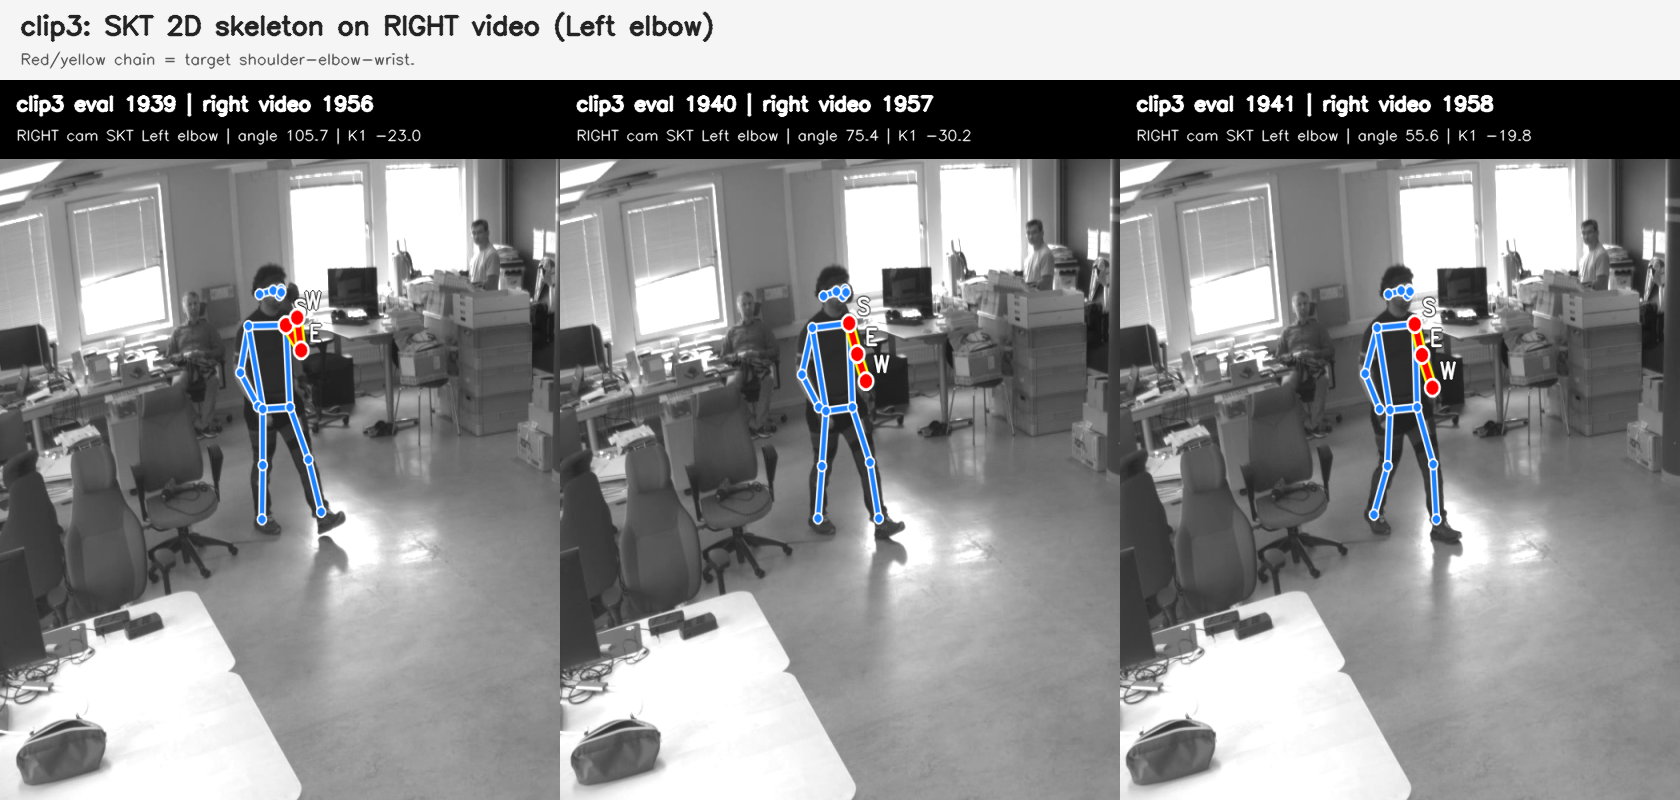
\includegraphics[width=\linewidth]{thesis_skt_high_delta_left_elbow_frames.png}
    \caption{Left-elbow high-delta interval.}
  \end{subfigure}

  \vspace{0.35cm}
  \begin{subfigure}[b]{0.98\linewidth}
    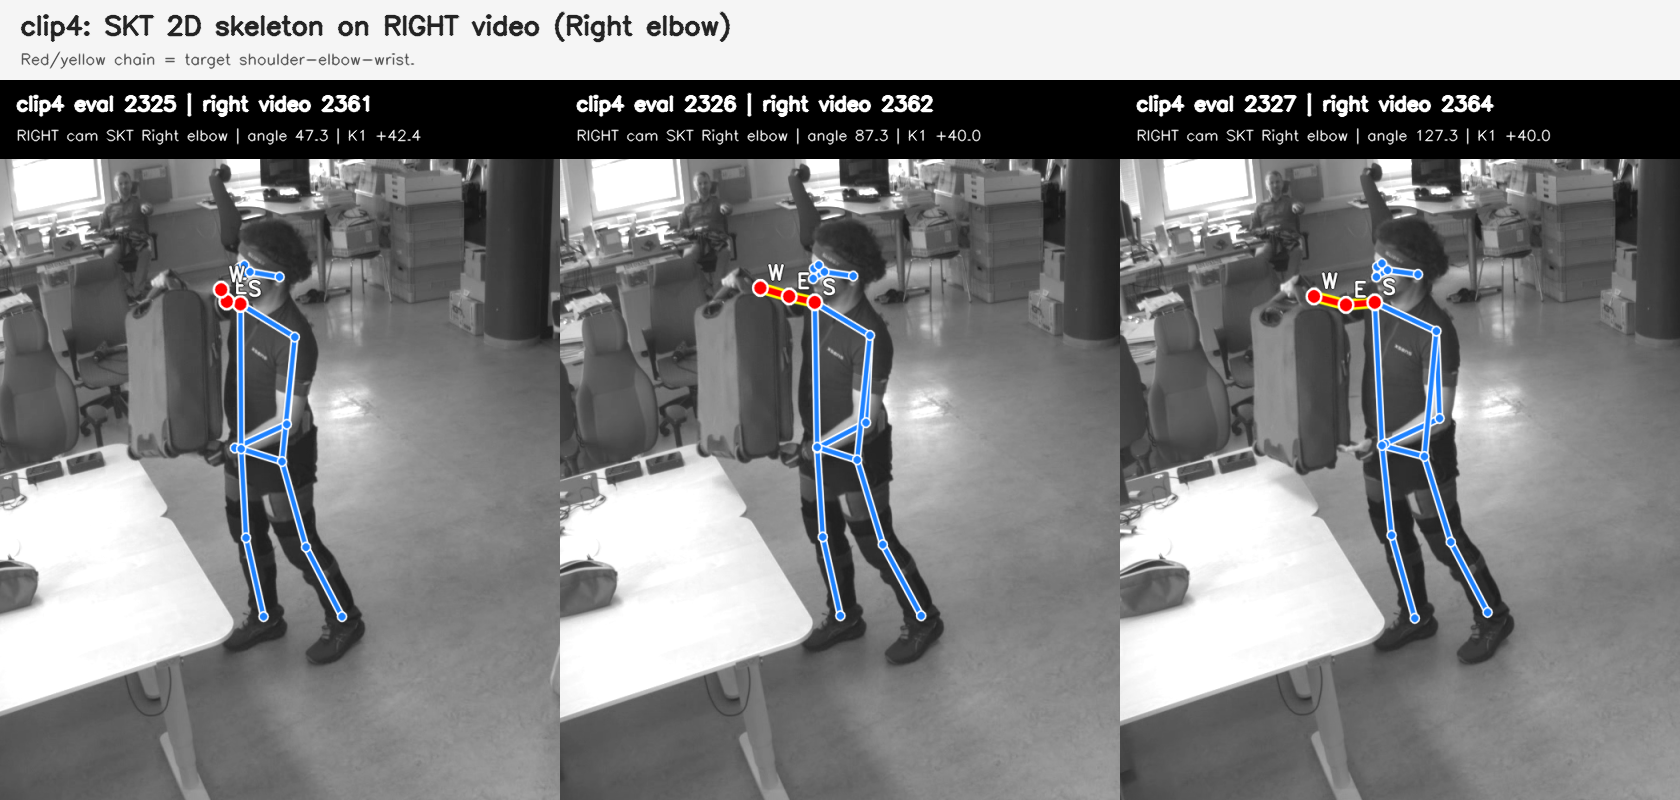
\includegraphics[width=\linewidth]{thesis_skt_high_delta_right_elbow_frames.png}
    \caption{Right-elbow high-delta interval.}
  \end{subfigure}
  \caption{Representative SKT high-delta diagnostic frames projected onto the original video view. These examples indicate that some large motion deltas are caused by local keypoint instability around the elbow chain rather than by physically implausible whole-body motion.}
  \label{fig:skt_high_delta_cases}
\end{figure}

\subsection{Limitations}

Four limitations of the present study set the boundary inside which all
quantitative results above should be read; they are stated explicitly here
so that the conclusion in Section~\ref{sec:conclusion} can rest on
honestly scoped evidence rather than on an over-generalised claim.
\emph{First}, all results come from a single subject performing a single
controlled recording in a manufacturing-like environment; the
between-method ranking should therefore be read as supported on this
dataset rather than as a general statement about every operator,
clothing style, lighting condition, or camera distance.
\emph{Second}, the deepest motion-space analysis focuses on the elbow,
which is the joint that the project investigated most carefully and the
joint whose Xsens calibration limitation is best quantified; the
motion-space numbers for the shoulder, hip, and knee are reported but
should be read with weaker confidence than the elbow numbers because
their reference floor is less well characterised.
\emph{Third}, the evaluation outputs depend on the smoothing window, the
segment-detection thresholds, and the constant-offset assumption used for
time alignment; the pipeline records these settings explicitly in the run
configuration so that any future work can rerun the same comparison under
different choices, and the synchronisation analysis in
Section~\ref{sec:data_setup} shows that the constant-offset assumption is
adequate for this recording but does not prove it for longer recordings.
\emph{Fourth}, Xsens is used throughout as an external comparison
reference and not as physical ground truth; the absolute angle errors are
therefore interpreted alongside the Xsens self-consistency floor
established in Section~\ref{sec:data_setup} rather than as direct error
against a true biomechanical zero.

\subsection{Implications for Real-time Deployment}

The deployment path that follows most cleanly from the above is to
prioritise getting the calibrated SKT pipeline running efficiently on
GPU hardware before treating learning-based pose models as
replacements rather than as optional stabilisers.
The concrete engineering steps are well-established: export the 2D pose
model to TensorRT, move video decoding and preprocessing onto the GPU,
and keep triangulation and joint-angle computation lightweight enough to
remain in the streaming budget; lightweight real-time pose models such
as RTMPose \cite{jiang2023rtmpose} make this direction realistic at the
2D-detection stage, although the final reportable number must be
end-to-end latency rather than model inference time alone, because
decoding, preprocessing, and post-processing each consume a measurable
share of the per-frame budget.
Once this baseline streams reliably, the two natural extensions are
(i) integrating a learning-based pose head -- of the FastSAM3D family --
as an optional smoothing or fallback signal when SKT quality flags drop
below an acceptable threshold, and (ii) introducing transformer-based
temporal priors to repair the keypoint-chain failures identified in the
high-delta analysis above; both extensions are framed here as
\emph{stabilisers on top of} the calibrated stereo baseline rather than
as replacements for it, because the deployment-geometry advantages
discussed in Section~7.2 do not transfer to a pure monocular pipeline
without additional scale/coordinate work.

\clearpage
% =============================================================
\section{Conclusion and Future Work}
\label{sec:conclusion}
% =============================================================

\subsection{Conclusion}

This thesis evaluates 3D human pose estimation for manufacturing-oriented
ergonomic monitoring using a three-axis framework -- angle-space,
motion-space, and position-space -- against an Xsens reference whose
calibration limitation is explicitly quantified rather than ignored.
On the single-subject manufacturing recording used here, the
learning-based monocular FastSAM3D pipeline delivers better
agreement-track numbers (mean angle MAE 15.4\degr\ vs.\ 17.6\degr; mean
K=6 motion Pearson 0.64 vs.\ 0.38; segment ROM error 14.9\degr\ vs.\
26.9\degr) than the calibrated stereo SKT pipeline.
SKT nevertheless retains the only metric-scale 3D output among the
evaluated pipelines and is the only pipeline that exposes per-frame
geometric quality signals usable for downstream quality gating, so it
remains the right choice when deployment requires real units or
self-reported reliability rather than only joint-angle smoothness.
The substantive conclusion is therefore not a single recommended method
but a deliberate split: learning-based monocular pose is competitive
when the deployment task is restricted to joint angles and short-term
motion, while calibrated stereo is necessary when the deployment task
extends to metric 3D scale and explainable per-frame quality, and a
future ergonomic monitoring system is likely to want both -- learned
priors for body-pose stability, stereo geometry for scale and
deployment transparency.

\subsection{Future Work}

Three follow-up directions are required before the present results can
be claimed as generally applicable rather than as evidence for a single
controlled recording.

\begin{enumerate}[leftmargin=1.2cm]
  \item \textbf{Validation on additional recordings and subjects.}
        Repeat the same three-axis protocol on at least one additional
        operator, additional clothing, additional lighting, and an
        unscripted task, in order to test whether the FastSAM3D
        agreement-track advantage generalises and whether the SKT
        high-delta failure modes recur in the same shoulder--elbow--wrist
        chain across subjects.
  \item \textbf{Real-time GPU deployment of SKT with optional learned
        stabilisers.} Move the SKT 2D backbone to TensorRT and the
        decoding/preprocessing onto the GPU, measure end-to-end streaming
        latency rather than model inference time alone, and then evaluate
        a FastSAM3D-style learned head as an optional smoothing or
        fallback signal triggered when SKT quality flags drop below the
        deployment threshold.
  \item \textbf{Beyond-elbow motion analysis and connection to a complete
        ergonomic risk score.} Extend the motion-space analysis to the
        shoulder, hip, and knee with the same reference-floor
        quantification that this thesis applies to the elbow, and then
        connect the resulting joint-angle stream to a full ergonomic
        risk score (e.g.\ RULA, REBA) rather than to RULA-bin agreement
        alone, so that pose-estimation quality and downstream
        risk-classification quality can be reported as a single
        deployment-relevant pipeline.
\end{enumerate}

\subsection{Recommended Next-stage Experimental Protocol}

To make the validation-on-new-datasets step above repeatable rather than
ad hoc, this subsection consolidates the working protocol used in the
present recording into a five-stage checklist
(Table~\ref{tab:validation_checklist}) that future datasets should run
\emph{in order}, with each stage gating the next.
The protocol enforces two methodological principles that emerged from
the present study.
The first principle is that data-ingestion integrity (orientation,
frame-ID re-pairing, timestamp monotonicity, calibration compatibility)
must be verified before any accuracy number is computed, because the
most expensive class of failure in the present pipeline is
mis-interpreting an ingestion bug as a pose-estimation result.
The second principle is that algorithmic changes and protocol changes
must be evaluated separately: if SKT is later modified with stronger
2D-keypoint filtering or a temporal repair module, the same K-frame
motion-delta protocol must be rerun before and after the modification
so that the comparison is fair, and if a new learning-based method is
added, its coordinate convention and filtering state must be recorded
before it is included in the position-space analysis.

\begin{table}[!htbp]
  \centering
  \caption{Five-stage validation checklist for extending the present thesis evaluation to new manufacturing recordings. Stages should be executed in order; each stage gates the next.}
  \label{tab:validation_checklist}
  \small
  \begin{tabularx}{\linewidth}{p{3.2cm}XX}
    \toprule
    Stage & What should be checked & Why it matters \\
    \midrule
    Dataset validation
    & Video orientation, hardware frame IDs, metadata timestamps, synchronised frame count, and camera calibration compatibility.
    & Prevents data-ingestion errors from being mis-interpreted as pose-estimation errors. \\
    Time alignment
    & Automatic offset curves on three independent scores, residual lag at the beginning and end of the recording, and common valid intervals.
    & Ensures that motion-space metrics compare the same physical movement period. \\
    Method comparison
    & Angle MAE, K-frame motion agreement at $K\in\{1,6,12,25\}$, segment ROM and DTW, and position-space diagnostics for every method.
    & Keeps the comparison multi-dimensional and avoids over-ranking methods by a single metric. \\
    Failure analysis
    & High-delta frames, occlusion cases, camera distance, and left--right keypoint consistency.
    & Connects quantitative outliers to concrete visual causes and guides targeted SKT repair work. \\
    Deployment check
    & End-to-end streaming latency, GPU preprocessing, model inference time, and stability under streaming input.
    & Tests whether the method can move from offline evaluation toward real-time ergonomic monitoring. \\
    \bottomrule
  \end{tabularx}
\end{table}

The final thesis version should therefore deliver two distinct kinds of
evidence rather than a single aggregate error number.
The first is \emph{quantitative agreement} across several recordings and
movement types, run through the checklist above so that the comparison
remains multi-dimensional and protocol-controlled.
The second is \emph{diagnostic evidence} that exposes when and why each
pipeline fails and which subsystem is responsible, of the kind that
Section~\ref{sec:discussion} presented for the SKT high-delta cases.
This combination is the right level of evidence for ergonomic deployment
in manufacturing, because a practical monitoring system needs not only
to be accurate on average but also to know -- and to expose -- when its
output should not be trusted.

\clearpage
% =============================================================
\appendix
\clearpage
% =============================================================

\section{Stereo Calibration Parameters}
\label{app:calibration}

The numerical calibration values reported below are the optimised parameters
that all SKT experiments in the thesis use as fixed input; the
binary form is stored at \texttt{shared/camera\_params.npz} and is loaded
directly by the pose pipeline.
The intrinsic matrices follow the OpenCV convention $K = [[f_x, 0, c_x];
[0, f_y, c_y]; [0,0,1]]$ in pixels, the distortion vectors follow the
14-parameter rational model used by OpenCV's \texttt{cv2.calibrateCamera}
(only the first 8 entries are non-zero in this calibration), and the
stereo extrinsics give the rotation $R$ and translation $T$ that map a
3D point from the left to the right camera frame in centimetres.

\begin{table}[!htbp]
  \centering
  \caption{Left and right camera intrinsic matrices (pixels) and the stereo extrinsic baseline.}
  \label{tab:calib_intrinsics}
  \small
  \begin{tabular}{lcc}
    \toprule
    Quantity & Left camera & Right camera \\
    \midrule
    $f_x$ (pixels)            & 1130.27 & 1129.01 \\
    $f_y$ (pixels)            & 1130.35 & 1129.63 \\
    $c_x$ (pixels)            & 1019.32 & 1028.31 \\
    $c_y$ (pixels)            &  825.72 &  826.35 \\
    \midrule
    Stereo baseline $\|T\|$   & \multicolumn{2}{c}{41.27\,cm} \\
    Image resolution          & \multicolumn{2}{c}{2048 $\times$ 1536} \\
    Distortion model          & \multicolumn{2}{c}{OpenCV rational (14-parameter)} \\
    \bottomrule
  \end{tabular}
\end{table}

The stereo rotation $R$ deviates from the identity by less than 0.011
radians on each off-diagonal entry, consistent with a near-aligned
parallel-baseline rig, and the translation vector
$T \approx [-41.27, -0.03, 0.04]^T$\,cm confirms that the baseline is
dominated by the $x$ axis as designed.
The essential matrix $E$ and fundamental matrix $F$ recorded in
\texttt{camera\_params.npz} are derived from $R$ and $T$ together with
the two intrinsic matrices and are not duplicated here.
The full distortion coefficients and the original calibration session
metadata (target type, number of valid views, per-view reprojection
residuals) are stored alongside the matrices in the same NPZ file.

\FloatBarrier
\clearpage
\section{Sensitivity Analyses}
\label{app:sensitivity}

The headline numbers reported in Section~\ref{sec:results} depend on
three parameter choices made in the evaluation pipeline: the camera-side
smoothing window, the activity-segment detection threshold, and the
DTW preprocessing convention.
This appendix reports how the SKT motion and segment-level numbers move
when each choice is varied, so that the reader can judge how brittle the
conclusion is.

\begin{table}[!htbp]
  \centering
  \caption{Sensitivity of SKT motion-space and segment-level numbers to the camera-side moving-average smoothing window, on the present recording. The 200\,ms and 300\,ms rows are identical because both round to a 3-frame centred window at 12.5\,fps.}
  \label{tab:sens_smoothing}
  \footnotesize
  \setlength{\tabcolsep}{4pt}
  \resizebox{\linewidth}{!}{%
  \begin{tabular}{lcccc}
    \toprule
    Window & Frames & SKT K=6 Pearson (L/R) & SKT ROM MAE (L/R, \degr) & K=1 quiet std (L/R, \degr) \\
    \midrule
    100\,ms & 1 & -- / --   & 38.4 / 33.3 & --   / --   \\
    200\,ms & 3 & 0.41 / 0.40 & 19.3 / 21.3 & 7.0 / 6.6 \\
    300\,ms & 3 & 0.41 / 0.40 & 19.3 / 21.3 & 7.0 / 6.6 \\
    400\,ms & 5 & 0.43 / 0.42 & 16.4 / 21.8 & 4.4 / 4.5 \\
    \bottomrule
  \end{tabular}%
  }
\end{table}

The 200\,ms working point chosen in the main body is the
literature-supported rule of thumb for non-explosive human motion; a
400\,ms window further reduces SKT quiet-frame jitter below the
$<$5\degr/frame validation target at the cost of a slightly weaker
short-term motion signal, and is reported here as the
``conservative-smoothing'' alternative for future runs.

\begin{table}[!htbp]
  \centering
  \caption{Sensitivity of detected segment counts to the activity-detection threshold (applied to the Xsens-derived reference K-frame deltas).}
  \label{tab:sens_segments}
  \small
  \begin{tabular}{lcc}
    \toprule
    Activity threshold (\degr) & Left-elbow segments & Right-elbow segments \\
    \midrule
    8  & 5  & 7  \\
    10 (default) & 8 & 9 \\
    12 & 13 & 15 \\
    \bottomrule
  \end{tabular}
\end{table}

Segment counts vary by a factor of roughly 2--3 across the tested
threshold range, but the cross-method ranking inside each row is stable:
FastSAM3D maintains the lowest segment ROM MAE and DTW distance
regardless of the threshold setting, so the main-body conclusion does
not depend on the specific threshold value chosen.
The DTW preprocessing sweep (\texttt{mean\_l2}, \texttt{mean}, and
\texttt{none}) confirms that the mean-subtracted, L2-normalised
convention adopted in the main body is the version under which the
XsensNative-vs-XsensFair anchor DTW remains near zero; without L2
normalisation the DTW distance becomes dominated by amplitude rather
than by shape, which is the explicit motivation for the chosen
preprocessing.

\FloatBarrier
\clearpage
\section{Implementation and Reproducibility Notes}
\label{app:repro}

The standalone evaluation workflow is implemented in
\texttt{00\_pose\_pipeline/}.
For the present dataset, the main reproduction command is:
\begin{footnotesize}
\begin{verbatim}
/opt/anaconda3/envs/pose/bin/python \
  00_pose_pipeline/src/run_pipeline.py \
  --config \
  00_pose_pipeline/configs/current_2025_ergonomics.yaml \
  --stages \
  validate,offset,angle,motion,segment,scatter
\end{verbatim}
\end{footnotesize}

The configuration file records the dataset-specific choices that
otherwise must be inferred from prose alone: the 180\degr\ video
rotation, the hardware-frame-ID synchronisation rule, the metadata
timestamp-parsing convention, the calibration NPZ path, the per-system
smoothing settings, the K-frame list $\{1,6,12,25\}$, the
activity-detection threshold, and the automatic offset-search range.
Generated outputs are stored under \texttt{00\_pose\_pipeline/runs/}
and include both the headline tables/figures referenced from the main
body and the per-stage diagnostics that drive Section~\ref{sec:discussion}.

Figure~\ref{fig:residual_lag_check} reports a residual lag diagnostic
that the pipeline can produce after the selected constant offset has
been applied; it is not a headline result but it documents the
sanity-check evidence used to defend the constant-offset assumption in
Section~\ref{sec:data_setup}.

\begin{figure}[!htbp]
  \centering
  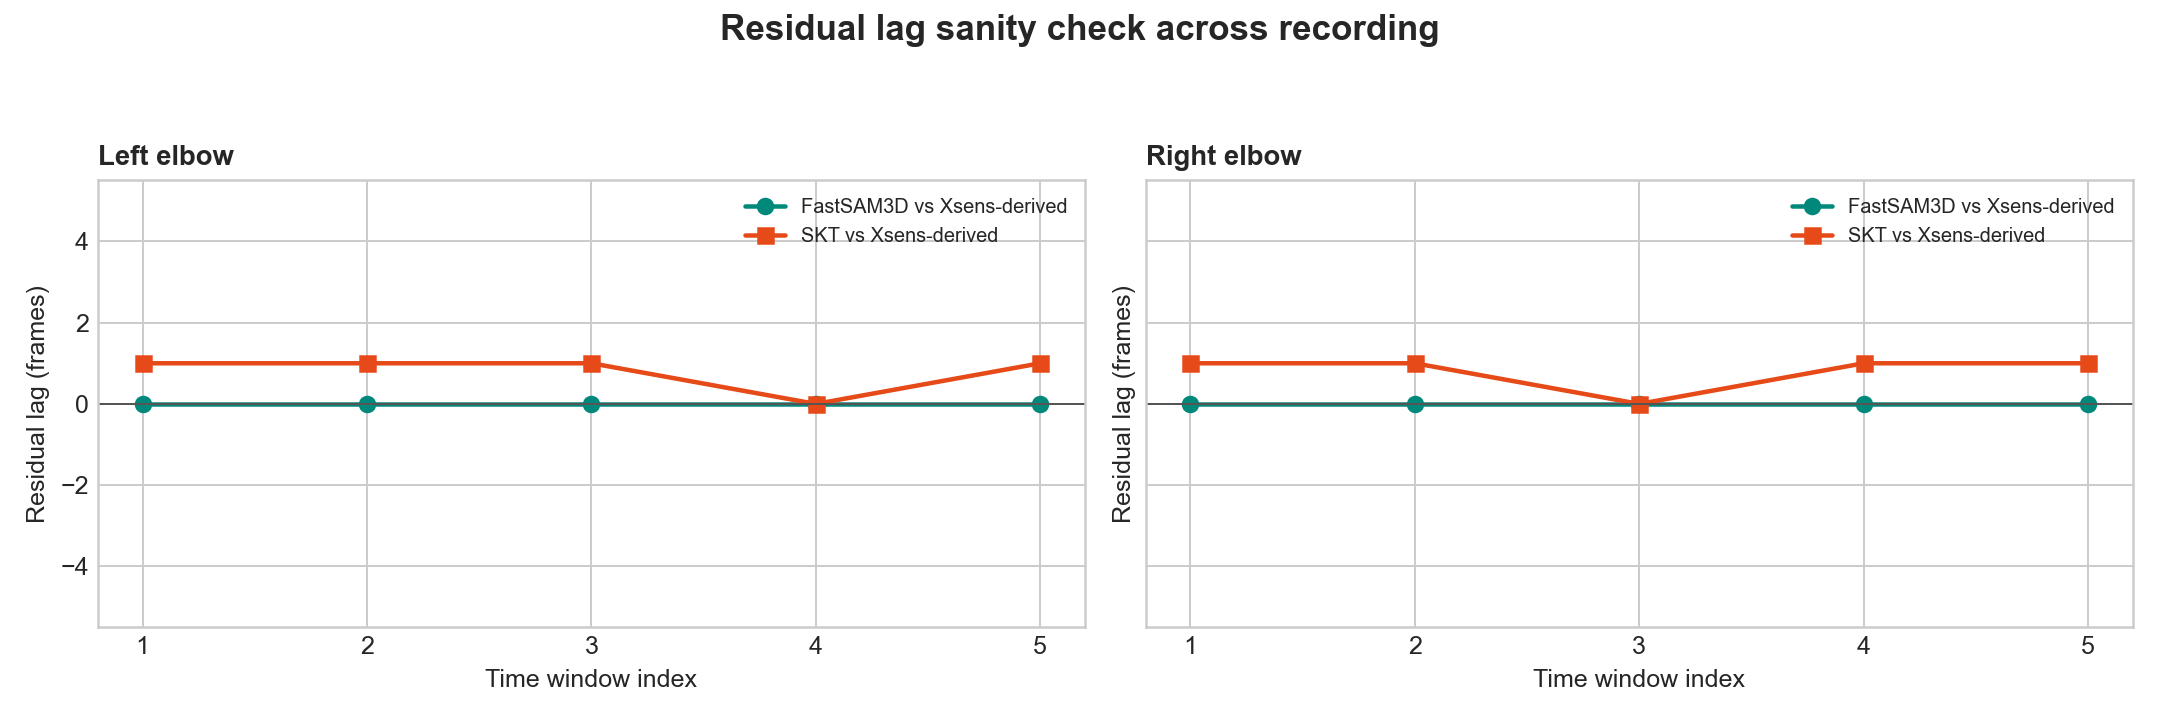
\includegraphics[width=\linewidth]{thesis_residual_lag_drift_check.png}
  \caption{Residual lag sanity check after applying the selected constant offset. The figure supports the assumption that a constant offset is adequate for the present recording, while explicitly acknowledging that future longer or multi-take recordings should rerun this check.}
  \label{fig:residual_lag_check}
\end{figure}

\FloatBarrier
\clearpage
\section{Claim-evidence Self-review}
\label{app:claim_evidence}

The table below maps every major thesis claim back to its supporting
evidence in this draft, following the
``Claim $|$ Evidence $|$ Status'' convention recommended for
adversarial paper review.
Claims marked \emph{Needs evidence} are stated as open items rather
than as supported conclusions, and the conclusion in
Section~\ref{sec:conclusion} is restricted to the claims marked
\emph{Supported}.

\begin{table}[H]
  \centering
  \caption{Claim-evidence map for the present thesis draft.}
  \label{tab:claim_evidence}
  \small
  \renewcommand{\arraystretch}{1.12}
  \begin{tabularx}{\linewidth}{p{4.0cm}Xp{1.9cm}}
    \toprule
    Claim & Evidence used in this draft & Status \\
    \midrule
    FastSAM3D is stronger than SKT in angle-space on the present dataset.
    & Table~\ref{tab:angle_summary} and Figure~\ref{fig:angle_summary_plot}: 15.4\degr\ mean MAE vs.\ 17.6\degr.
    & Supported \\
    FastSAM3D is stronger than SKT in K=6 motion-space agreement.
    & Table~\ref{tab:motion_summary}, Figure~\ref{fig:motion_k6_summary_plot}, and Figure~\ref{fig:k6_elbow_scatter}: mean Pearson 0.644 vs.\ 0.379; elbow correlations 0.54/0.69 vs.\ 0.39/0.39.
    & Supported \\
    SKT retains a position-space and interpretability advantage.
    & Table~\ref{tab:position_summary}, Figure~\ref{fig:position_diagnostic_plot}, and the SKT method design; SKT uses calibrated stereo scale and exposes per-frame geometric quality signals.
    & Supported \\
    A constant cross-system offset is adequate for the current recording.
    & Figure~\ref{fig:offset_search}, Figure~\ref{fig:first_last_delta}, and Figure~\ref{fig:residual_lag_check}; the three independent offset scores converge within $\sim$0.04\,s.
    & Supported for present recording \\
    SKT high-delta points are caused by local keypoint-chain instability.
    & Figure~\ref{fig:skt_high_delta_cases}: diagnostic frames show partial wrist occlusion, large camera distance, and inconsistent left/right elbow-chain detection during the high-delta intervals.
    & Supported qualitatively \\
    The SKT vs FastSAM3D ranking is robust to smoothing and segmentation parameters.
    & Appendix~\ref{app:sensitivity}: sensitivity tables across smoothing windows and activity thresholds preserve the FastSAM3D $>$ SKT ranking.
    & Supported \\
    Results generalise to manufacturing environments broadly.
    & Only one controlled single-subject dataset is evaluated.
    & Needs evidence \\
    Full RULA automation is solved.
    & Only continuous angle MAE and RULA-like bin agreement are reported; RULA scoring requires additional load/twist/repetition information.
    & Not claimed \\
    \bottomrule
  \end{tabularx}
\end{table}

\clearpage

\begin{thebibliography}{99}

\bibitem{mcatamney1993rula}
L.~McAtamney and E.~N.~Corlett,
\textit{RULA: a survey method for the investigation of work-related upper limb disorders},
Applied Ergonomics, vol.~24, no.~2, pp.~91--99, 1993.

\bibitem{menolotto2020motion}
M.~Menolotto, D.-S.~Komaris, S.~Tedesco, B.~O'Flynn, and M.~Walsh,
\textit{Motion capture technology in industrial applications: A systematic review},
Sensors, vol.~20, no.~19, article 5687, 2020.

\bibitem{yu2019joint}
Y.~Yu, X.~Yang, H.~Li, X.~Luo, and H.~Guo,
\textit{Joint-level vision-based ergonomic assessment tool for construction workers},
Journal of Construction Engineering and Management, vol.~145, no.~5, 2019.

\bibitem{menanno2024ergonomic}
M.~Menanno, C.~Riccio, V.~Benedetto, and G.~Palmieri,
\textit{An ergonomic risk assessment system based on 3D human pose estimation and collaborative robot},
Applied Sciences, vol.~14, no.~11, article 4823, 2024.

\bibitem{quesada2026supporting}
A.~Quesada Diaz, A.~Iriondo Pascual, L.~Hanson, D.~H{\"o}gberg, and A.~Syberfeldt,
\textit{Supporting ergonomics evaluations in manufacturing: A comparison of computer vision- and IMU-based motion capture},
IOP Conference Series: Materials Science and Engineering, vol.~1342, article 012053, 2026.

\bibitem{iriondo2024development}
A.~Iriondo Pascual, L.~Hanson, D.~H{\"o}gberg, E.~Brolin, and A.~Syberfeldt,
\textit{Development and initial usability evaluation of a digital tool for simulation-based multi-objective optimization of productivity and worker well-being},
Advanced Engineering Informatics, vol.~60, article 102726, 2024.

\bibitem{iriondo2025integrating}
A.~Iriondo Pascual, L.~Hanson, E.~Brolin, D.~H{\"o}gberg, and A.~Syberfeldt,
\textit{Integrating motion capture and digital human modelling tools for worker ergonomics assessment: A case study from experimental lab to real-world manufacturing},
Lecture Notes in Computer Science, vol.~15828, pp.~324--333, 2025.

\bibitem{filippeschi2017survey}
A.~Filippeschi, N.~Schmitz, M.~Miezal, G.~Bleser, E.~Ruffaldi, and D.~Stricker,
\textit{Survey of motion tracking methods based on inertial sensors: A focus on upper limb human motion},
Sensors, vol.~17, no.~6, article 1257, 2017.

\bibitem{roetenberg2009xsens}
D.~Roetenberg, H.~Luinge, and P.~Slycke,
\textit{Xsens MVN: Full 6DOF human motion tracking using miniature inertial sensors},
Xsens Technologies technical report, 2009.

\bibitem{cao2019openpose}
Z.~Cao, G.~Hidalgo, T.~Simon, S.-E.~Wei, and Y.~Sheikh,
\textit{OpenPose: Realtime multi-person 2D pose estimation using part affinity fields},
IEEE Transactions on Pattern Analysis and Machine Intelligence,
vol.~43, no.~1, pp.~172--186, 2019.

\bibitem{jiang2023rtmpose}
T.~Jiang, P.~Lu, L.~Zhang, N.~Ma, R.~Han, C.~Lyu, Y.~Li, and K.~Chen,
\textit{RTMPose: Real-time multi-person pose estimation based on MMPose},
arXiv preprint arXiv:2303.07399, 2023.

\bibitem{pavllo20193d}
D.~Pavllo, C.~Feichtenhofer, D.~Grangier, and M.~Auli,
\textit{3D human pose estimation in video with temporal convolutions and semi-supervised training},
Proceedings of the IEEE/CVF Conference on Computer Vision and Pattern Recognition, pp.~7753--7762, 2019.

\bibitem{zhu2023motionbert}
W.~Zhu, X.~Ma, Z.~Liu, L.~Liu, W.~Wu, and Y.~Wang,
\textit{MotionBERT: A unified perspective on learning human motion representation},
Proceedings of the IEEE/CVF International Conference on Computer Vision, pp.~15085--15099, 2023.

\bibitem{yang2026fastsam3d}
T.~Yang, S.~He, H.~Jing, J.~Yang, Z.~Liu, C.~Zou, and Y.~Wang,
\textit{Fast SAM 3D Body: Accelerating SAM 3D Body for Real-Time Full-Body Human Mesh Recovery},
arXiv preprint arXiv:2603.15603, 2026.

\bibitem{hartley2004multiple}
R.~Hartley and A.~Zisserman,
\textit{Multiple View Geometry in Computer Vision},
2nd ed., Cambridge University Press, 2004.

\bibitem{hirschmuller2007sgbm}
H.~Hirschm{\"u}ller,
\textit{Stereo processing by semiglobal matching and mutual information},
IEEE Transactions on Pattern Analysis and Machine Intelligence,
vol.~30, no.~2, pp.~328--341, 2007.

\bibitem{kabsch1976solution}
W.~Kabsch,
\textit{A solution for the best rotation to relate two sets of vectors},
Acta Crystallographica, Section A, vol.~32, pp.~922--923, 1976.

\bibitem{sakoe1978dtw}
H.~Sakoe and S.~Chiba,
\textit{Dynamic programming algorithm optimization for spoken word recognition},
IEEE Transactions on Acoustics, Speech, and Signal Processing,
vol.~26, no.~1, pp.~43--49, 1978.

\bibitem{perezluque2026reaching}
E.~P{\'e}rez Luque, S.~Lee, D.~H{\"o}gberg, J.~Yang, and M.~Lamb,
\textit{Predicting human upper extremity reaching motions: Comparison of optimization-based method and heuristic method},
International Journal of Human--Computer Interaction, 2026.
DOI: 10.1080/10447318.2026.2632154.

\end{thebibliography}

\end{document}

% =============================================================

\documentclass[12pt,a4paper]{article}

\usepackage[margin=2.5cm]{geometry}
\usepackage{fontspec}
\defaultfontfeatures{Ligatures=TeX}
\usepackage{amsmath,amssymb}
\usepackage{siunitx}
\usepackage{booktabs}
\usepackage{graphicx}
\usepackage{subcaption}
\usepackage[table]{xcolor}
\usepackage{hyperref}
\usepackage{microtype}
\usepackage{parskip}
\usepackage{enumitem}
\usepackage{array}
\usepackage{float}
\usepackage{tabularx}
\usepackage{setspace}
\usepackage{placeins}
\usepackage{caption}

\hypersetup{colorlinks=true, linkcolor=blue!70!black, urlcolor=blue!70!black, citecolor=green!50!black}
\graphicspath{{figures/}}
\emergencystretch=2em
\setstretch{1.06}
\setlength{\textfloatsep}{1.1em plus 0.25em minus 0.2em}
\setlength{\floatsep}{1.0em plus 0.25em minus 0.2em}
\setlength{\intextsep}{1.0em plus 0.25em minus 0.2em}
\captionsetup{font=small, labelfont=bf}

\definecolor{goodcolor}{rgb}{0.00,0.38,0.18}
\definecolor{warncolor}{rgb}{0.55,0.27,0.07}
\definecolor{badcolor}{rgb}{0.65,0.10,0.10}
\newcommand{\good}[1]{\textcolor{goodcolor}{\textbf{#1}}}
\newcommand{\warn}[1]{\textcolor{warncolor}{\textbf{#1}}}
\newcommand{\bad}[1]{\textcolor{badcolor}{\textbf{#1}}}
\newcommand{\degr}{\ensuremath{^\circ}}

\title{\textbf{Posture and Activity Detection in Manufacturing Environments\\Using 3D Vision and AI}}
\author{Fanbo Meng\\
\small Chalmers University of Technology\\
\small In collaboration with Viscando AB}
\date{Master's Thesis Draft, June 2026}

\begin{document}
\maketitle
\tableofcontents
\newpage

% =============================================================
\section*{Abstract}
% =============================================================

Ergonomic risk assessment in manufacturing demands pose-estimation systems
that are spatially accurate, temporally consistent, and interpretable at the
joint-angle level, yet the dominant evaluation practice in the pose-estimation
literature still relies on a single distance metric such as Mean Per-Joint
Position Error, which is not sufficient to decide whether a method is fit for
ergonomic monitoring.
This thesis revisits 3D human pose estimation for manufacturing settings by
comparing a calibrated stereo keypoint triangulation pipeline (SKT) with a
monocular learning-based pipeline (FastSAM3D); an Xsens inertial motion-capture
suit is used as an external reference system rather than as absolute ground
truth, because its body-model calibration introduces systematic angle offsets
that must be acknowledged in the evaluation design.
The evaluation is organized around three complementary axes -- angle-space
accuracy, motion-space consistency, and position-space geometry -- and the
motion-space axis is built on K-frame angle deltas
($\Delta_K\theta_t = \theta_t-\theta_{t-K}$), which cancel the static Xsens
offset by differencing and expose true short-term motion agreement.
On a single-subject manufacturing recording of 2801 synchronized stereo frame
pairs over 248.8\,s, FastSAM3D achieves lower mean angle MAE than SKT across
eight body angles (15.4\degr\ vs.\ 17.6\degr) and stronger K=6 motion-delta
correlation with the Xsens-derived reference (mean Pearson 0.64 vs.\ 0.38;
right-elbow Pearson 0.69 vs.\ 0.39).
This angle and motion advantage is attributed to FastSAM3D's learned
body-shape and motion-continuity priors, which absorb anatomical constraints
from large training corpora and consequently suppress the per-frame keypoint
jitter that a frame-independent geometric triangulation pipeline propagates
directly into its angle estimates.
SKT, by contrast, retains a clear position-space advantage: its 3D coordinates
inherit metric scale directly from the calibrated stereo baseline without any
external alignment step, and the per-frame geometric quality signals it
exposes~-- epipolar error, reprojection error, triangulation confidence~--
provide deployment-ready reliability indicators that a monocular learning-based
pipeline does not offer natively.
These findings indicate that the two approaches are complementary rather than
interchangeable: learned monocular pose estimation is the more competitive
choice when angle accuracy and temporal motion smoothness are the primary
requirements, while calibrated stereo triangulation remains essential when
metric 3D coordinates and transparent per-frame reliability are needed for
downstream ergonomic quality control.

% =============================================================
\newpage
\section{Introduction}
% =============================================================

\subsection{Motivation}

Work-related musculoskeletal disorders remain one of the dominant
occupational-health burdens in manufacturing, and the established
countermeasure is repeated ergonomic risk assessment of operators while they
perform actual production tasks.
The standard observational instruments for such assessment, including the
Rapid Upper Limb Assessment (RULA), depend on a trained observer who manually
classifies joint postures into discrete risk categories
\cite{mcatamney1993rula}; this practice is labour-intensive, observer
dependent, and impossible to deploy at the temporal resolution that modern
just-in-time production demands.
Camera-based 3D human pose estimation offers a path toward continuous,
non-intrusive ergonomic monitoring, because the joint angles needed for RULA
and similar instruments can in principle be read directly from a body
skeleton reconstructed from video.

Realising this promise on the factory floor changes what counts as ``good''
pose estimation.
The dominant benchmarks in the pose-estimation literature reward
visually-plausible skeletons and low Mean Per-Joint Position Error (MPJPE) on
short, well-lit, frontal-view clips; an ergonomic monitoring system, however,
must produce joint-angle estimates that are temporally stable across long
shifts, robust to occlusion and dark workwear, and traceable to interpretable
quality signals when downstream automated risk scoring is involved.
This thesis therefore treats pose estimation as a measurement problem that
sits between multi-view geometry, learning-based vision, and application-level
ergonomic evaluation, and it organises its evaluation around the properties
that ergonomic deployment actually requires rather than around a single
geometric distance metric.

\subsection{Problem Statement and Scope}

The thesis investigates 3D body-keypoint and joint-angle estimation from a
calibrated stereo camera setup in a manufacturing-like environment, with the
deployment target being downstream ergonomic risk monitoring rather than
generic motion reconstruction.
The primary pose-estimation method developed in the thesis is Sparse
Keypoint Triangulation (SKT), in which a 2D pose detector is run on
synchronised left and right video streams and the matched keypoints are
triangulated into 3D under the calibrated stereo geometry; the study then
benchmarks SKT against a monocular learning-based pipeline (FastSAM3D).

A central methodological constraint is that no laboratory-grade optical
motion-capture system was available for the full manufacturing recording, so
this thesis adopts an Xsens inertial suit as an \emph{external reference
system}, deliberately avoiding the language of ``absolute ground truth''.
This wording is not cosmetic: the Xsens body model is calibrated through a
short on-subject procedure that can absorb true global orientation and
introduce a systematic per-joint offset, most visibly at the elbow.
Reporting only absolute joint-angle MAE against such a reference therefore
risks transferring the reference's calibration bias into a verdict about the
vision pipeline, and the evaluation design must counter this by reporting
relative-change metrics (frame-to-frame K-frame angle deltas) in parallel
with absolute angles, since differencing cancels any static offset that the
two systems may carry.

\subsection{Research Questions}

The thesis is structured around three research questions:

\begin{enumerate}[label=\textbf{RQ\arabic*:}, leftmargin=1.8cm]
  \item How accurately can a calibrated stereo keypoint triangulation
        pipeline (SKT) recover the eight ergonomically relevant upper- and
        lower-body joint angles in a manufacturing-style recording, when
        absolute and motion-space accuracy are reported in parallel against
        an Xsens-derived reference?
  \item Under a unified evaluation protocol (shared timeline, common
        smoothing policy, identical reference), how does the geometry-based
        SKT pipeline compare with the learning-based FastSAM3D pipeline in
        (i) absolute angle accuracy and (ii) K-frame motion consistency at
        $K\in\{1,6,12,25\}$ frames?
  \item Which pipeline properties beyond raw accuracy -- in particular
        per-frame quality signals, metric scale, and resilience to
        occlusion and low-texture industrial backgrounds -- decide whether
        a method is fit for real-time ergonomic monitoring on GPU hardware?
\end{enumerate}

\subsection{Contributions}

In addressing the three research questions, the thesis makes the following
contributions:

\begin{itemize}[leftmargin=1.2cm]
  \item \textbf{A reproducible stereo pose pipeline (SKT)} that combines
        synchronised 2D keypoint detection, calibrated DLT triangulation,
        three-point geometric joint-angle computation, and per-frame
        geometry-aware quality signals (triangulation confidence, epipolar
        error, reprojection error) that can drive downstream quality gating.
  \item \textbf{A three-axis evaluation framework} -- angle-space, motion-space,
        position-space -- that exposes method-property tradeoffs which a single
        MPJPE-style metric would conceal, and that is reusable across other
        vision pipelines on the same dataset.
  \item \textbf{An explicit cross-system synchronisation and filtering protocol},
        including automatic temporal-offset estimation against three independent
        scores, hardware-frame-ID re-pairing for non-monotonic stereo
        timestamps, and a per-system smoothing policy (no extra smoothing on
        the already heavily filtered Xsens reference, unified 200\,ms moving
        average on the camera-based methods).
  \item \textbf{An empirical comparison} that finds the monocular learning-based
        FastSAM3D pipeline more competitive than the calibrated stereo SKT on
        both angle MAE and K-frame motion correlation for this manufacturing
        recording, while showing that SKT retains an irreplaceable advantage
        in metric 3D scale and in geometry-aware quality control needed for
        deployment.
\end{itemize}

\subsection{Thesis Structure}

The remainder of the thesis is organised as follows.
Section~\ref{sec:background} reviews relevant work on 3D human pose
estimation, vision-based ergonomic assessment, and reference-system
limitations.
Section~\ref{sec:data_setup} describes the stereo capture system, the
2025 ergonomics dataset, the Xsens reference data, and the cross-system
time-synchronisation procedure.
Section~\ref{sec:methods} presents the two evaluated pose-estimation
pipelines (SKT and FastSAM3D).
Section~\ref{sec:evaluation} defines the three-axis evaluation framework and
the unified filtering policy.
Section~\ref{sec:results} reports the angle-space, motion-space,
segment-level, and position-space results, and synthesises them across
methods.
Section~\ref{sec:discussion} discusses applicability boundaries, failure
modes, and limitations, and
Section~\ref{sec:conclusion} concludes and outlines future work.

\clearpage
% =============================================================
\section{Background and Related Work}
\label{sec:background}
% =============================================================

\subsection{3D Human Pose Estimation}

3D human pose estimation recovers either explicit body keypoints or
parametric body-model parameters from one or several camera streams, and the
existing literature divides clearly along whether the recovery uses one view
or multiple views.
Monocular approaches estimate 3D pose from a single image or video, either
through a two-stage 2D--detection + 3D--lifting pipeline or through an
end-to-end regression that maps image features directly to 3D coordinates.
Real-time 2D pose estimators such as OpenPose and RTMPose have established
that the 2D detection stage can be made fast and accurate enough for online
use \cite{cao2019openpose,jiang2023rtmpose}, and temporal 3D models such as
VideoPose3D and MotionBERT have shown that body-motion priors can be learned
from large pose-sequence corpora and used to stabilise the lifting step
\cite{pavllo20193d,zhu2023motionbert}.
The structural limitation of any monocular pipeline, however, is that the
absolute distance from camera to subject is not directly observed; depth and
metric scale must be inferred from learned body proportions or recovered
through an external alignment step, which is acceptable for visual
animation but problematic for ergonomic measurement.

Stereo and multi-view approaches replace this scale ambiguity with explicit
multi-view geometry.
In a calibrated two-camera setup, an epipolar relation constrains where a
point seen in the left view must appear in the right view, and the intersection
of the two corresponding viewing rays gives a 3D coordinate that inherits its
scale directly from the measured baseline; this geometric chain, together with
the intrinsic and extrinsic camera matrices recovered during calibration,
forms the standard machinery of multi-view computer vision
\cite{hartley2004multiple}.
Stereo pipelines also split into a sparse and a dense branch: sparse
triangulation matches a small number of 2D keypoints across views and
triangulates each one independently, which is fast and interpretable but
sensitive to per-keypoint jitter and to left--right mismatches, whereas
dense disparity methods such as Semi-Global Block Matching estimate depth at
every pixel \cite{hirschmuller2007sgbm} and then read off the joint depths,
which gives a denser geometric description but degrades sharply on the
low-texture clothing and visually ambiguous backgrounds that are common in
real industrial scenes.

\subsection{Pose Evaluation Methodology}

Pose-estimation errors do not project equally onto every evaluation space,
and reporting only one metric can hide the property that actually matters
for the downstream application.
\emph{Position-space} evaluation, dominated in the literature by Mean
Per-Joint Position Error (MPJPE), measures the 3D Euclidean distance between
estimated and reference joints after rigid alignment, and it is the natural
metric when the goal is reconstruction geometry.
\emph{Angle-space} evaluation instead asks whether the joint angles computed
from the estimated skeleton are quantitatively correct, which is the
question that ergonomic risk instruments such as RULA actually answer
\cite{mcatamney1993rula}; a method can have low MPJPE while still placing
an elbow flexion in a different RULA risk bin, and the reverse is also
possible.
\emph{Motion-space} evaluation looks at the temporal change of pose, for
example through frame-to-frame angle deltas, and is the most useful axis when
the reference system itself carries a static calibration offset, because
differencing cancels that offset and isolates true motion agreement.
This thesis therefore reports all three axes and treats no single metric as
sufficient on its own.

The ergonomic side of the evaluation is anchored by RULA, a screening
instrument that maps upper-limb and body postures to discrete risk
categories based on joint-angle ranges \cite{mcatamney1993rula}.
Because RULA depends primarily on angles rather than on absolute 3D
positions, the thesis treats RULA-like bin agreement as an
\emph{application-level classification metric} for selected joints alongside
the continuous angle MAE; it deliberately does not claim to implement a
complete automated RULA scoring system, since full RULA also requires
external information about loads, twisting, and repetition that the vision
pipeline alone cannot infer.
This narrower scope keeps the comparison focused on the pose-estimation
component while still connecting it to the deployment intent.

Vision-based ergonomic assessment has been studied increasingly in recent
years, and systematic reviews note that motion-capture technologies are
becoming common in industrial workplaces but that deployment quality still
depends on usability, measurement reliability, and task-specific
interpretation \cite{menolotto2020motion}.
Concrete vision-based ergonomic systems have been proposed in
construction \cite{yu2019joint} and in collaborative-robot settings
\cite{menanno2024ergonomic}, and the most directly relevant comparison study
to this thesis is the work of Quesada Diaz, Iriondo Pascual, and co-authors,
who explicitly compared computer-vision and IMU-based motion capture for
manufacturing ergonomics and highlighted the same recurrent themes of
careful filtering, cross-system alignment, and reference-aware benchmarking
that this thesis adopts \cite{quesada2026supporting}.
Iriondo Pascual's broader work on simulation-based productivity and
worker-wellbeing optimisation further situates the present thesis within
human-centred manufacturing and digital ergonomics
\cite{iriondo2024development,iriondo2025integrating}.

\subsection{Reference Systems}

The evaluation of any vision pose pipeline ultimately depends on what counts
as the reference, and inertial motion-capture systems such as Xsens have
become the practical default outside the optical-mocap laboratory because
they record high-frequency full-body motion without external cameras or
markers \cite{roetenberg2009xsens,filippeschi2017survey}.
The same convenience, however, is the source of the systematic limitation
that motivates the evaluation design of this thesis: the Xsens body-model
calibration is performed through a short on-subject N-pose / T-pose
procedure that absorbs the true global orientation and resets each segment
into the system's internal reference frame, and the resulting per-joint
angles can therefore carry an unknown static offset relative to a true
biomechanical zero, an effect that is particularly visible at the elbow.
For this reason the thesis consistently treats Xsens as an
\emph{external comparison / reference system} rather than as absolute
ground truth, and reserves the language of physical ground truth for
higher-grade systems such as optical mocap or per-joint goniometry that are
outside the scope of the present recording.

Within the Xsens output itself the thesis distinguishes between
\emph{Xsens native} joint angles, which are read directly from the MVNX
joint-angle channel and follow the Xsens body model and its internal
conventions, and \emph{Xsens-derived geometric} angles, which are
re-computed from the Xsens 3D segment positions using the same three-point
formula that is later applied to all vision pipelines.
The Xsens-derived geometric representation is adopted as the main reference
throughout the thesis because it removes the angle-definition mismatch
between systems, and because its agreement with the native representation
(MAE $\approx$ 2\degr\ in motion-space on the present recording) supplies a
quantitative lower-bound that calibrates how to interpret the absolute
errors reported for the vision methods.

\subsection{Related Work Summary and Positioning}

The closest prior work compares an IMU suit with a single vision pipeline
on industrial-style tasks \cite{quesada2026supporting} and concludes that
vision is promising but that filtering and alignment must be reported
carefully; the present thesis extends this line in three concrete ways.
First, it benchmarks two independently produced vision pipelines
side-by-side on the same recording -- a calibrated sparse-stereo pipeline
(SKT) and a monocular learning-based pipeline (FastSAM3D) -- so that the
geometry-versus-learning tradeoff is quantified rather than asserted.
Second, it replaces the single-metric evaluation that dominates the
pose-estimation literature with an explicit three-axis framework
(angle / motion / position), and it makes the motion axis robust to
reference-system calibration offsets by reporting K-frame angle deltas at
multiple time scales.
Third, it treats reference-system limitations as a first-class methodological
concern: the thesis quantifies the Xsens self-consistency floor on the same
metrics that are applied to the vision pipelines, so that every reported
number can be read against the lower bound of what the reference itself can
support.
The contribution is therefore not a new pose-estimation algorithm but a
deployment-oriented evaluation protocol, together with the empirical finding
that on this dataset learning-based monocular pose is competitive on angle
and motion while calibrated stereo retains an irreplaceable role in metric
scale and geometry-aware quality control.

\clearpage
% =============================================================
\section{Data and Experimental Setup}
\label{sec:data_setup}
% =============================================================

\subsection{Stereo Capture System}

All recordings used in this thesis come from a synchronised two-camera
stereo rig operated by Viscando AB.
Each camera captures at 2048$\times$1536 pixels and a nominal frame rate of
12.5\,fps, and the two streams are time-tagged at acquisition with a
hardware frame identifier together with a microsecond-resolution metadata
timestamp; the hardware identifier is what makes a robust left--right pairing
possible later, because the metadata timestamps alone can drift on either
side.
Because the cameras are physically mounted upside-down in the production
fixture, every frame is rotated by 180\degr\ before pose estimation is run,
so that gravity-up matches the assumption of the downstream pose detector
and skeleton orientation.

\subsection{Camera Calibration}

The geometric chain that maps a pair of 2D keypoints into a 3D coordinate
relies on accurate camera calibration, and small calibration errors are
amplified twice -- first when the rays are triangulated and again when three
3D points are turned into an angle -- so calibration quality is treated here
as a first-class methodological input rather than as a routine setup step.
The current calibration was estimated from an asymmetric circular-dot
target under a rational distortion model and yields a stereo baseline of
41.27\,cm with sub-pixel reprojection residuals on the calibration images;
the full intrinsic, distortion, and extrinsic matrices are reported in
Appendix~A and are treated as fixed inputs for all SKT
experiments in this thesis.

Figure~\ref{fig:calibration_evolution} documents the calibration refinement
that led to the current parameters and shows why the refinement was
necessary.
The first calibration attempt produced a geometrically consistent stereo
pair but estimated a baseline that was visibly off the measured physical
baseline of the rig, together with a reprojection error above the
working threshold that downstream triangulation can tolerate; the refined
and finally optimised calibration moved the estimated baseline back onto
the physical value and pushed the reprojection error into the sub-pixel
range, which is the regime in which the SKT pipeline produces stable
angle estimates rather than amplified jitter.

\begin{figure}[!htbp]
  \centering
  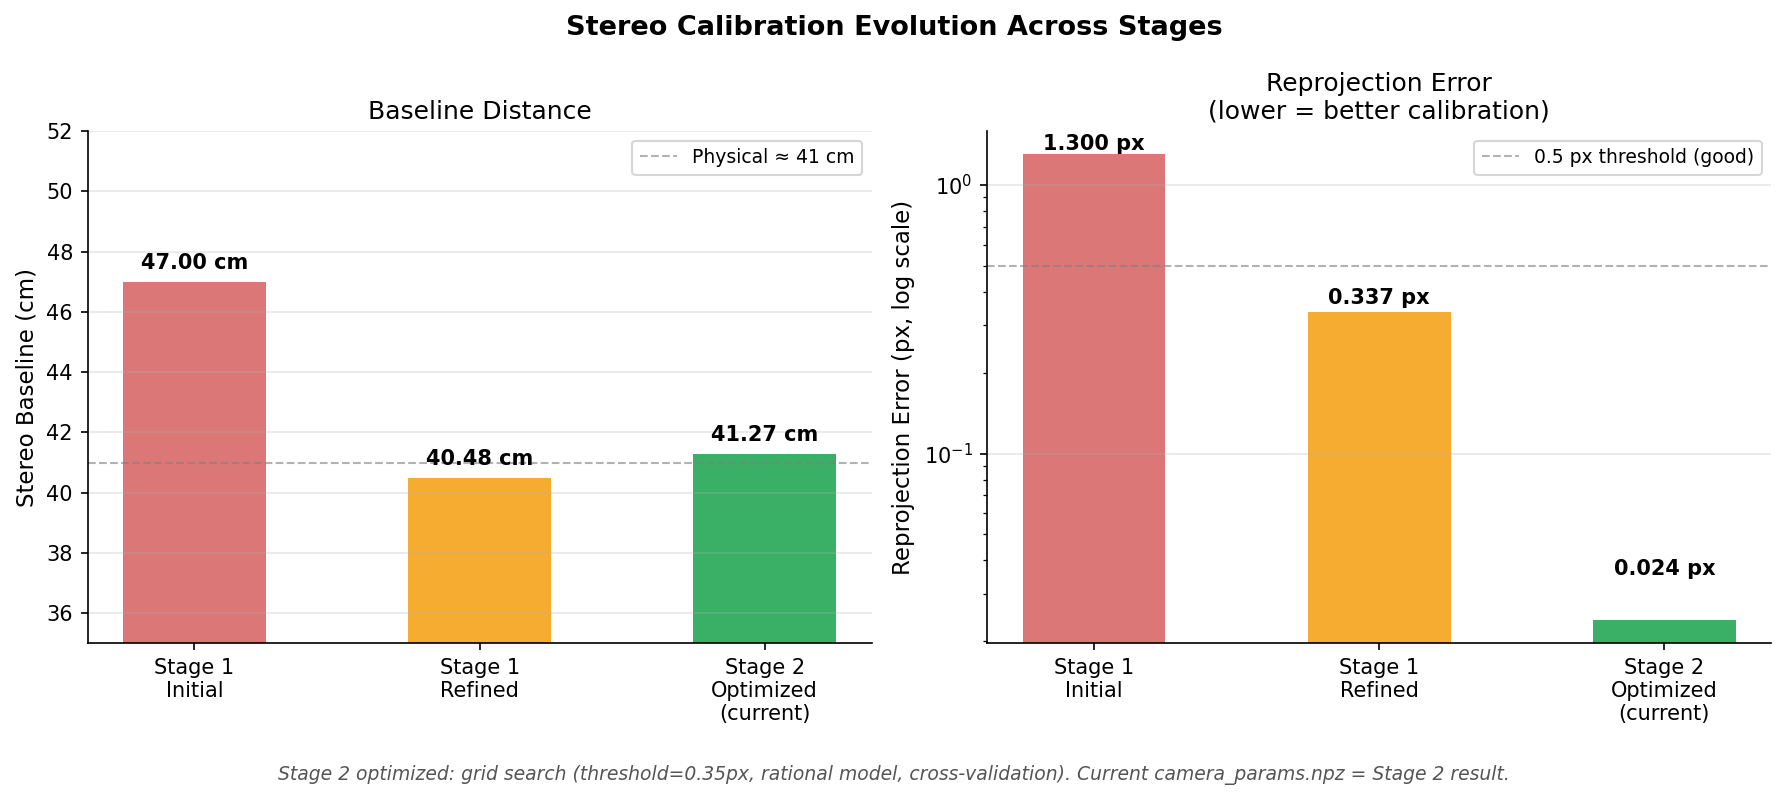
\includegraphics[width=\linewidth]{calibration_evolution.png}
  \caption{Stereo calibration evolution. The current calibration balances a realistic baseline estimate with a low reprojection error, making it suitable as the fixed geometric input for SKT.}
  \label{fig:calibration_evolution}
\end{figure}

\subsection{2025 Ergonomics Dataset}

All quantitative results in this thesis are computed on a single
single-subject ergonomics recording collected in a controlled
manufacturing-like environment, and this is therefore the dominant
generalisability limitation of the present study.
The subject performs a representative mix of factory-floor activities --
walking, sitting, squatting, reaching, lifting, and interacting with
furniture -- so that all major upper- and lower-body postures are exercised
within a single contiguous take rather than as isolated short clips.
After left--right pairing by hardware frame identifier, the usable
synchronised camera timeline contains 2801 frame pairs spanning 248.8\,s,
which corresponds to an effective frame rate of 12.5\,fps; the left raw
metadata contains 3015 rows and the right raw metadata contains 2882 rows,
so a non-trivial fraction of each side is either unpaired or falls outside
the synchronised interval, which is exactly what motivates the explicit
hardware-ID re-pairing step rather than reliance on raw row indices.
Table~\ref{tab:timeline_summary} summarises the resulting working timeline
that all downstream evaluations share.

\begin{table}[!htbp]
  \centering
  \caption{Summary of the synchronized camera timeline used for evaluation.}
  \label{tab:timeline_summary}
  \begin{tabular}{lc}
    \toprule
    Quantity & Value \\
    \midrule
    Synchronized frame pairs & 2801 \\
    Duration & 248.8 s \\
    Median frame interval & 0.0800 s \\
    Effective frame rate & 12.50 fps \\
    Left metadata rows & 3015 \\
    Right metadata rows & 2882 \\
    Rotation applied & 180\degr \\
    \bottomrule
  \end{tabular}
\end{table}

\subsection{Xsens Reference Data and Angle Representations}

The Xsens recording supplies full-body motion data on an independent time
axis and contains two distinct angle representations that the thesis must
choose between before any cross-method comparison can be reported.
The first is the \emph{Xsens native} joint-angle output, which is read
directly from the MVNX joint-angle channels and follows the Xsens body
model together with its internal axis and zero conventions.
The second is the \emph{Xsens-derived geometric} angle representation, in
which the joint angles are re-computed from the Xsens 3D segment positions
using the same three-point arccosine formula that is later applied to the
vision pipelines; this representation is adopted as the main reference
throughout the thesis because it removes the angle-definition mismatch
between the reference and the vision methods at the cost of being a
slightly less direct read of the Xsens body model.

The comparison between the two Xsens representations is then re-used as a
quantitative reference-system sanity check rather than discarded.
At the elbow, the two representations agree to within approximately
1--1.5\degr\ MAE in absolute angle space, and they agree to a Pearson
correlation of $\sim$0.99 in K-frame motion space; at the shoulder and hip,
the agreement is visibly weaker because the underlying axis conventions
differ more.
The implication for the thesis evaluation design is two-fold.
First, the elbow numbers serve as a \emph{lower-bound anchor}: a vision
method whose absolute angle MAE against Xsens-derived geometric is several
times the elbow self-consistency floor is unlikely to be limited by the
reference, whereas one that approaches the floor is approaching the
information limit of the reference itself.
Second, the larger shoulder/hip mismatch is one of the reasons the thesis
reports motion-space metrics alongside absolute angle MAE, since
differencing cancels both the unknown global Xsens calibration offset and
much of the axis-definition mismatch between the two representations.

\subsection{Cross-system Time Synchronisation}

Cross-system synchronisation is unavoidable for the present setup because
the cameras and the Xsens suit run on independent clocks, and any
mis-alignment converts directly into degraded motion-space agreement, so
the thesis adopts an automatic three-score offset search rather than a
manually picked shift.
The procedure first sweeps the offset coarsely between 0 and 30\,s, then
refines around the best candidate; at every candidate it computes three
independent agreement scores -- a position-space score on the 3D segment
positions, an angle-space score on the joint angles, and a motion-delta
score on the K-frame angle deltas -- and selects the motion-delta optimum
as the final offset because the motion evaluation is the most sensitive of
the three to residual sub-second mis-alignment.

For the present recording, the selected offset is 17.31\,s, and the
position-, angle-, and motion-delta optima fall at 17.27\,s, 17.28\,s, and
17.31\,s respectively.
The fact that three scores derived from three independent error spaces
converge inside a window of about 0.04\,s is the strongest evidence
available in this thesis that a single constant offset is an adequate
alignment model for this recording: had the underlying clock relation been
non-constant, the three scores would not be expected to peak so close
together.
Figure~\ref{fig:offset_search} shows the score curves produced by the
search and visualises this triple agreement.

\begin{figure}[!htbp]
  \centering
  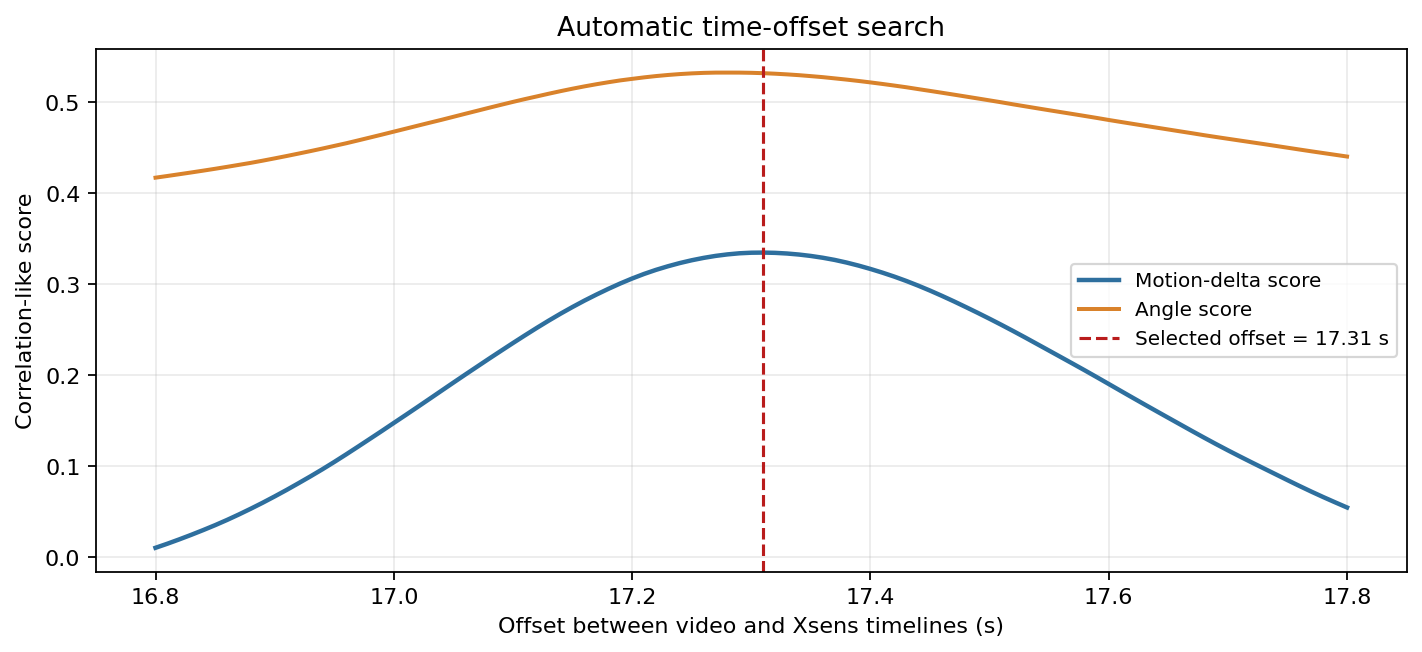
\includegraphics[width=\linewidth]{thesis_offset_search.png}
  \caption{Automatic offset estimation between the camera timeline and the Xsens reference timeline. The final selected value is 17.31 s, with position-, angle-, and motion-based scores all supporting a similar alignment.}
  \label{fig:offset_search}
\end{figure}

A second, qualitative synchronisation check is provided by overlaying the
aligned elbow-angle curves from all systems on the shared timeline
(Figure~\ref{fig:angle_time_alignment}).
The purpose of this plot is not to rank methods at the angle level -- that
is the task of Section~\ref{sec:results} -- but to confirm that the main
movement phases of the recording line up across systems after the offset
has been applied, so that any residual short-term deviation can be
attributed to true method behaviour rather than to an unfixed global shift.

\begin{figure}[!htbp]
  \centering
  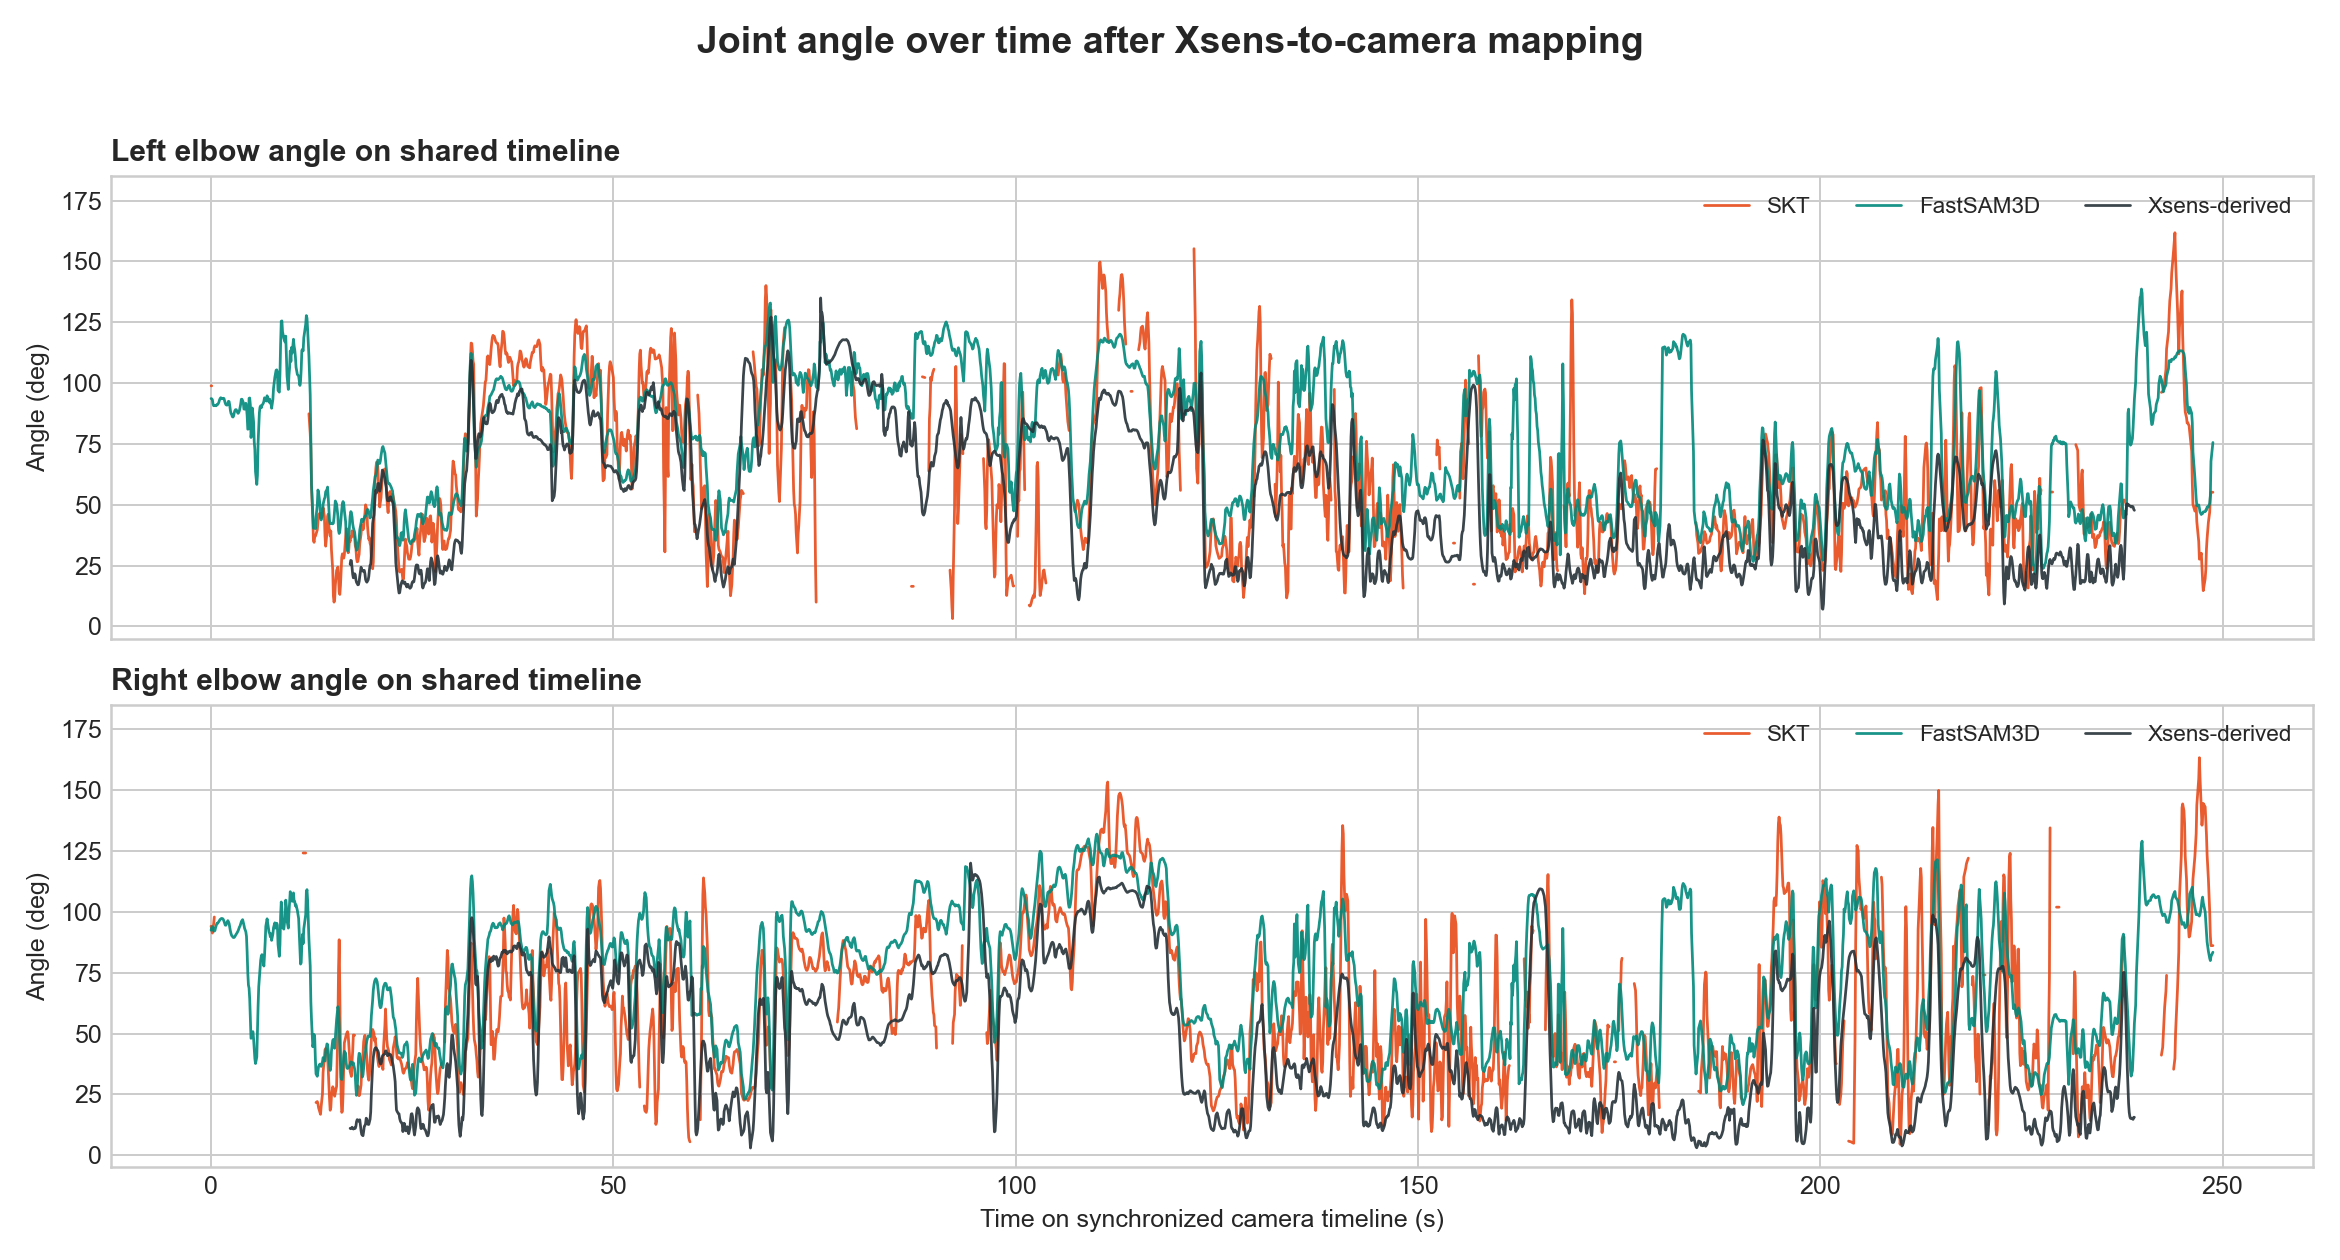
\includegraphics[width=\linewidth]{thesis_joint_angle_over_time.png}
  \caption{Left and right elbow angles on the shared timeline after offset correction. The plot provides a qualitative synchronisation check before quantitative angle and motion metrics are interpreted.}
  \label{fig:angle_time_alignment}
\end{figure}

A third check addresses the possibility that, even with a near-perfect
mean offset, the camera and Xsens clocks could drift slowly over the
$\sim$4\,min recording.
Figure~\ref{fig:first_last_delta} compares the K=6 motion-delta windows at
the beginning and end of the common valid interval; had the underlying
drift been large, the late-interval deltas would be expected to lose their
alignment with the reference even though the early-interval deltas still
agree.
The check is qualitative rather than a formal drift estimate, but the
observed late-interval agreement is comparable to the early-interval
agreement, which supports the use of a single constant offset for the
remainder of the thesis while explicitly acknowledging that future longer
or multi-take recordings should repeat this check.

\begin{figure}[!htbp]
  \centering
  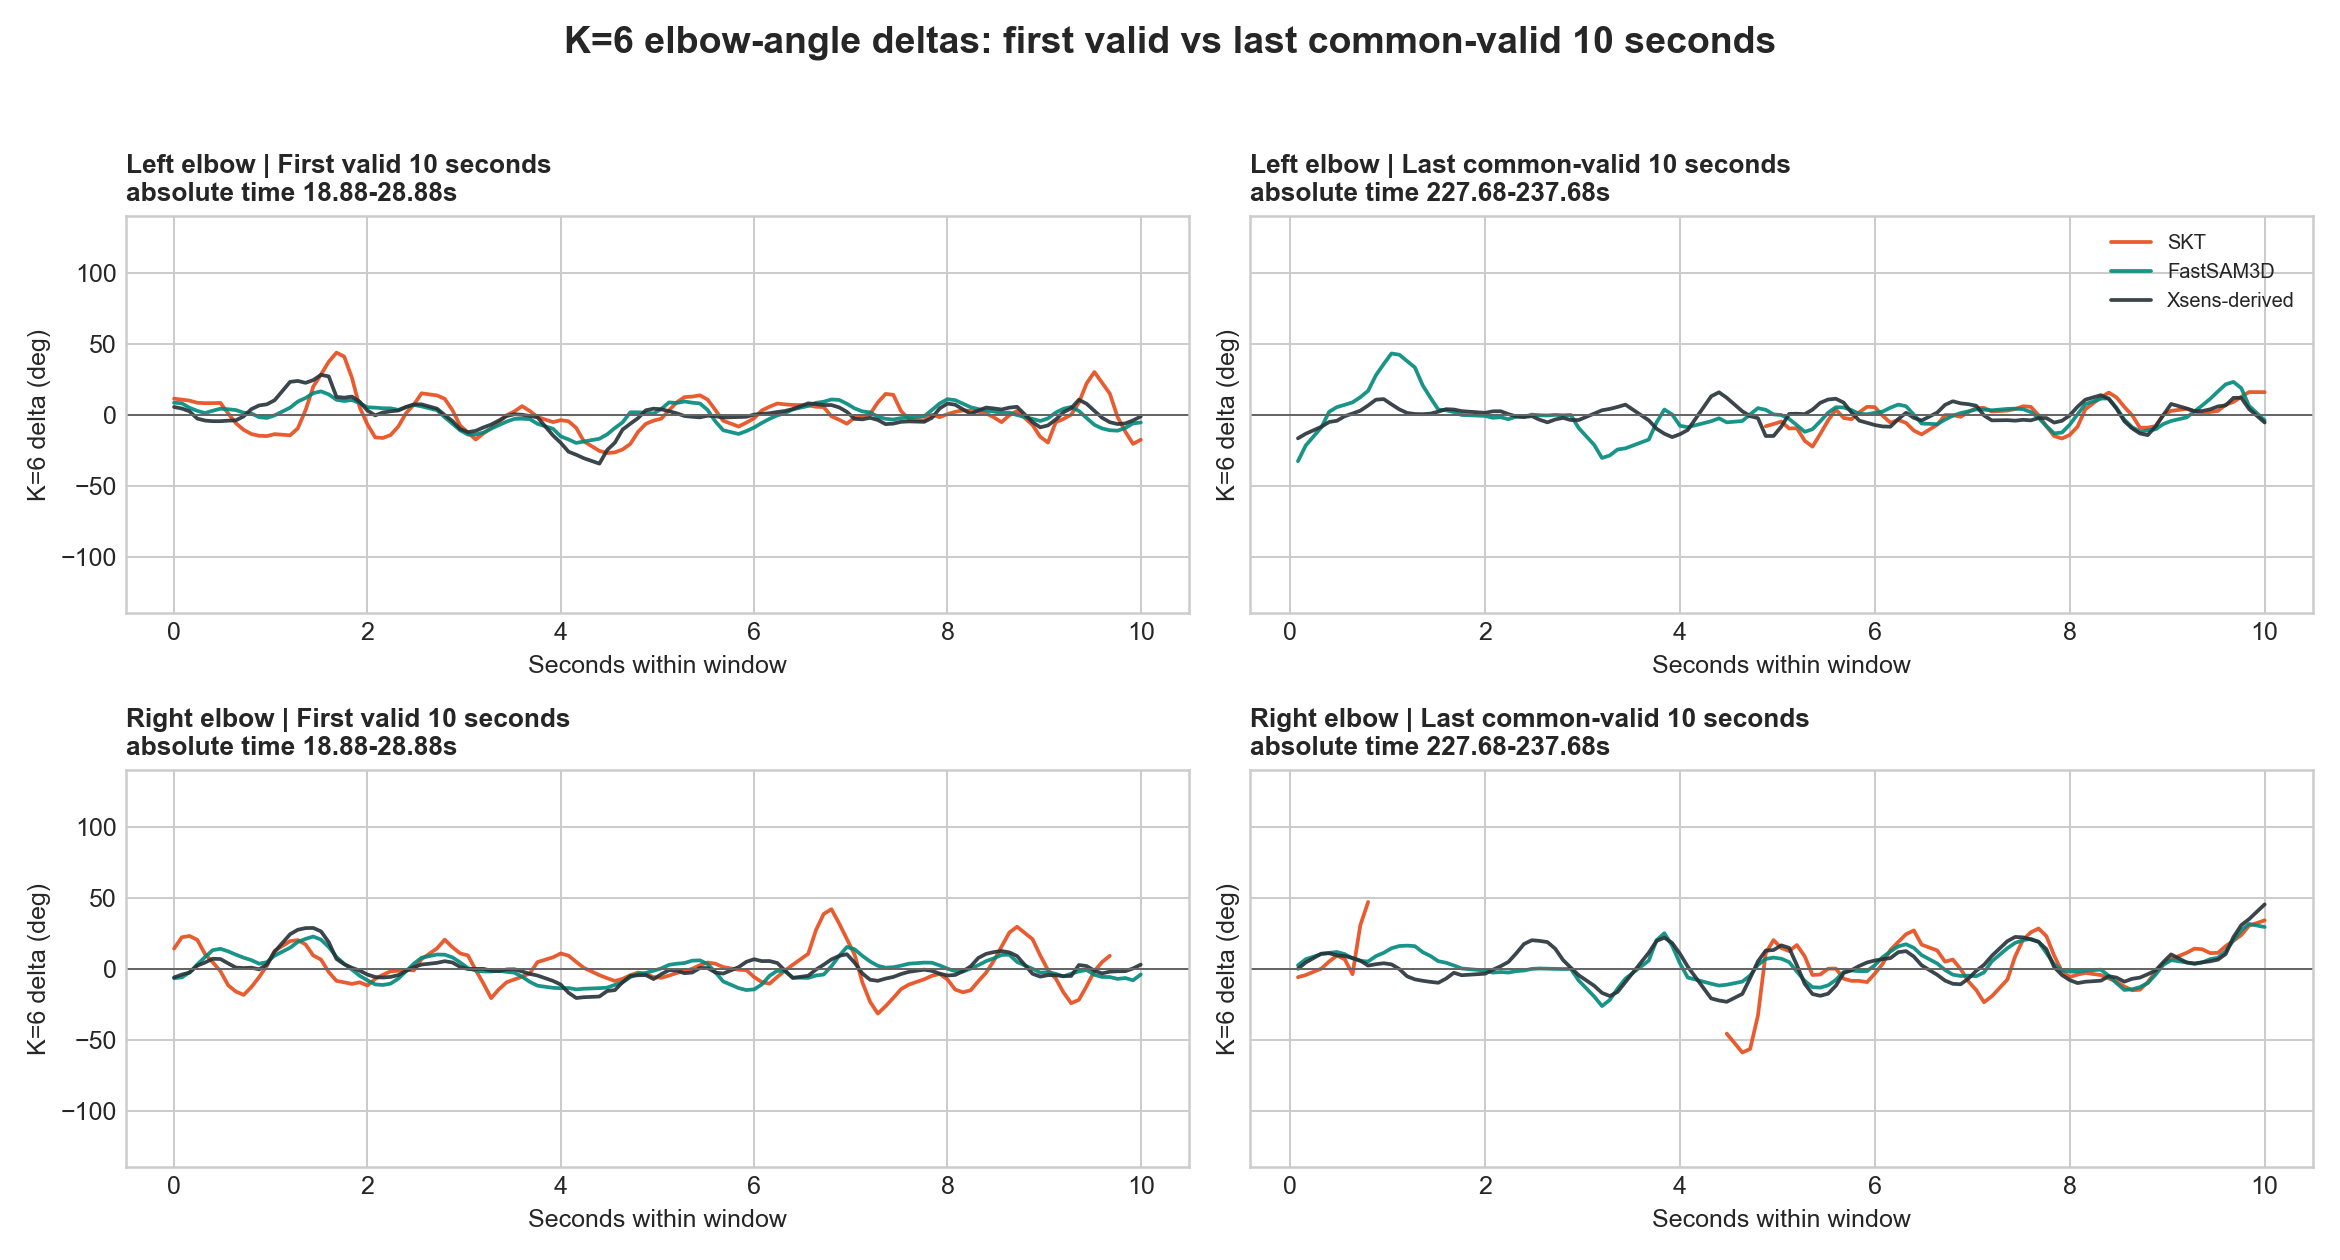
\includegraphics[width=\linewidth]{thesis_k6_delta_first_last_10s.png}
  \caption{K=6 elbow motion deltas near the beginning and end of the common valid interval. This figure is used as a practical check that the chosen constant offset remains reasonable across the recording.}
  \label{fig:first_last_delta}
\end{figure}

\clearpage
% =============================================================
\section{Methods}
\label{sec:methods}
% =============================================================

\subsection{Overview}

The thesis benchmarks two pose-estimation pipelines against the same Xsens
reference and the same evaluation protocol: SKT, the primary calibrated
sparse-stereo method developed in this thesis, and FastSAM3D, the monocular
learning-based alternative.
Figure~\ref{fig:pipeline_overview} shows the full experimental flow, and
Table~\ref{tab:method_roles} summarises each pipeline's input assumption, main
advantage, and main risk.

The single design choice that matters most for interpreting the rest of the
thesis is the deliberate separation between pose estimation and evaluation.
Both methods are mapped onto the same shared timeline and judged with
the same metrics, but those metrics are then split across two independent
axes (angle, motion) rather than collapsed into a single ranking
score; this prevents the recurring failure mode in which a method that is
strong in one space, for example metric stereo geometry, is implicitly
assumed to be equally strong in temporal angle consistency.

\begin{figure}[!htbp]
  \centering
  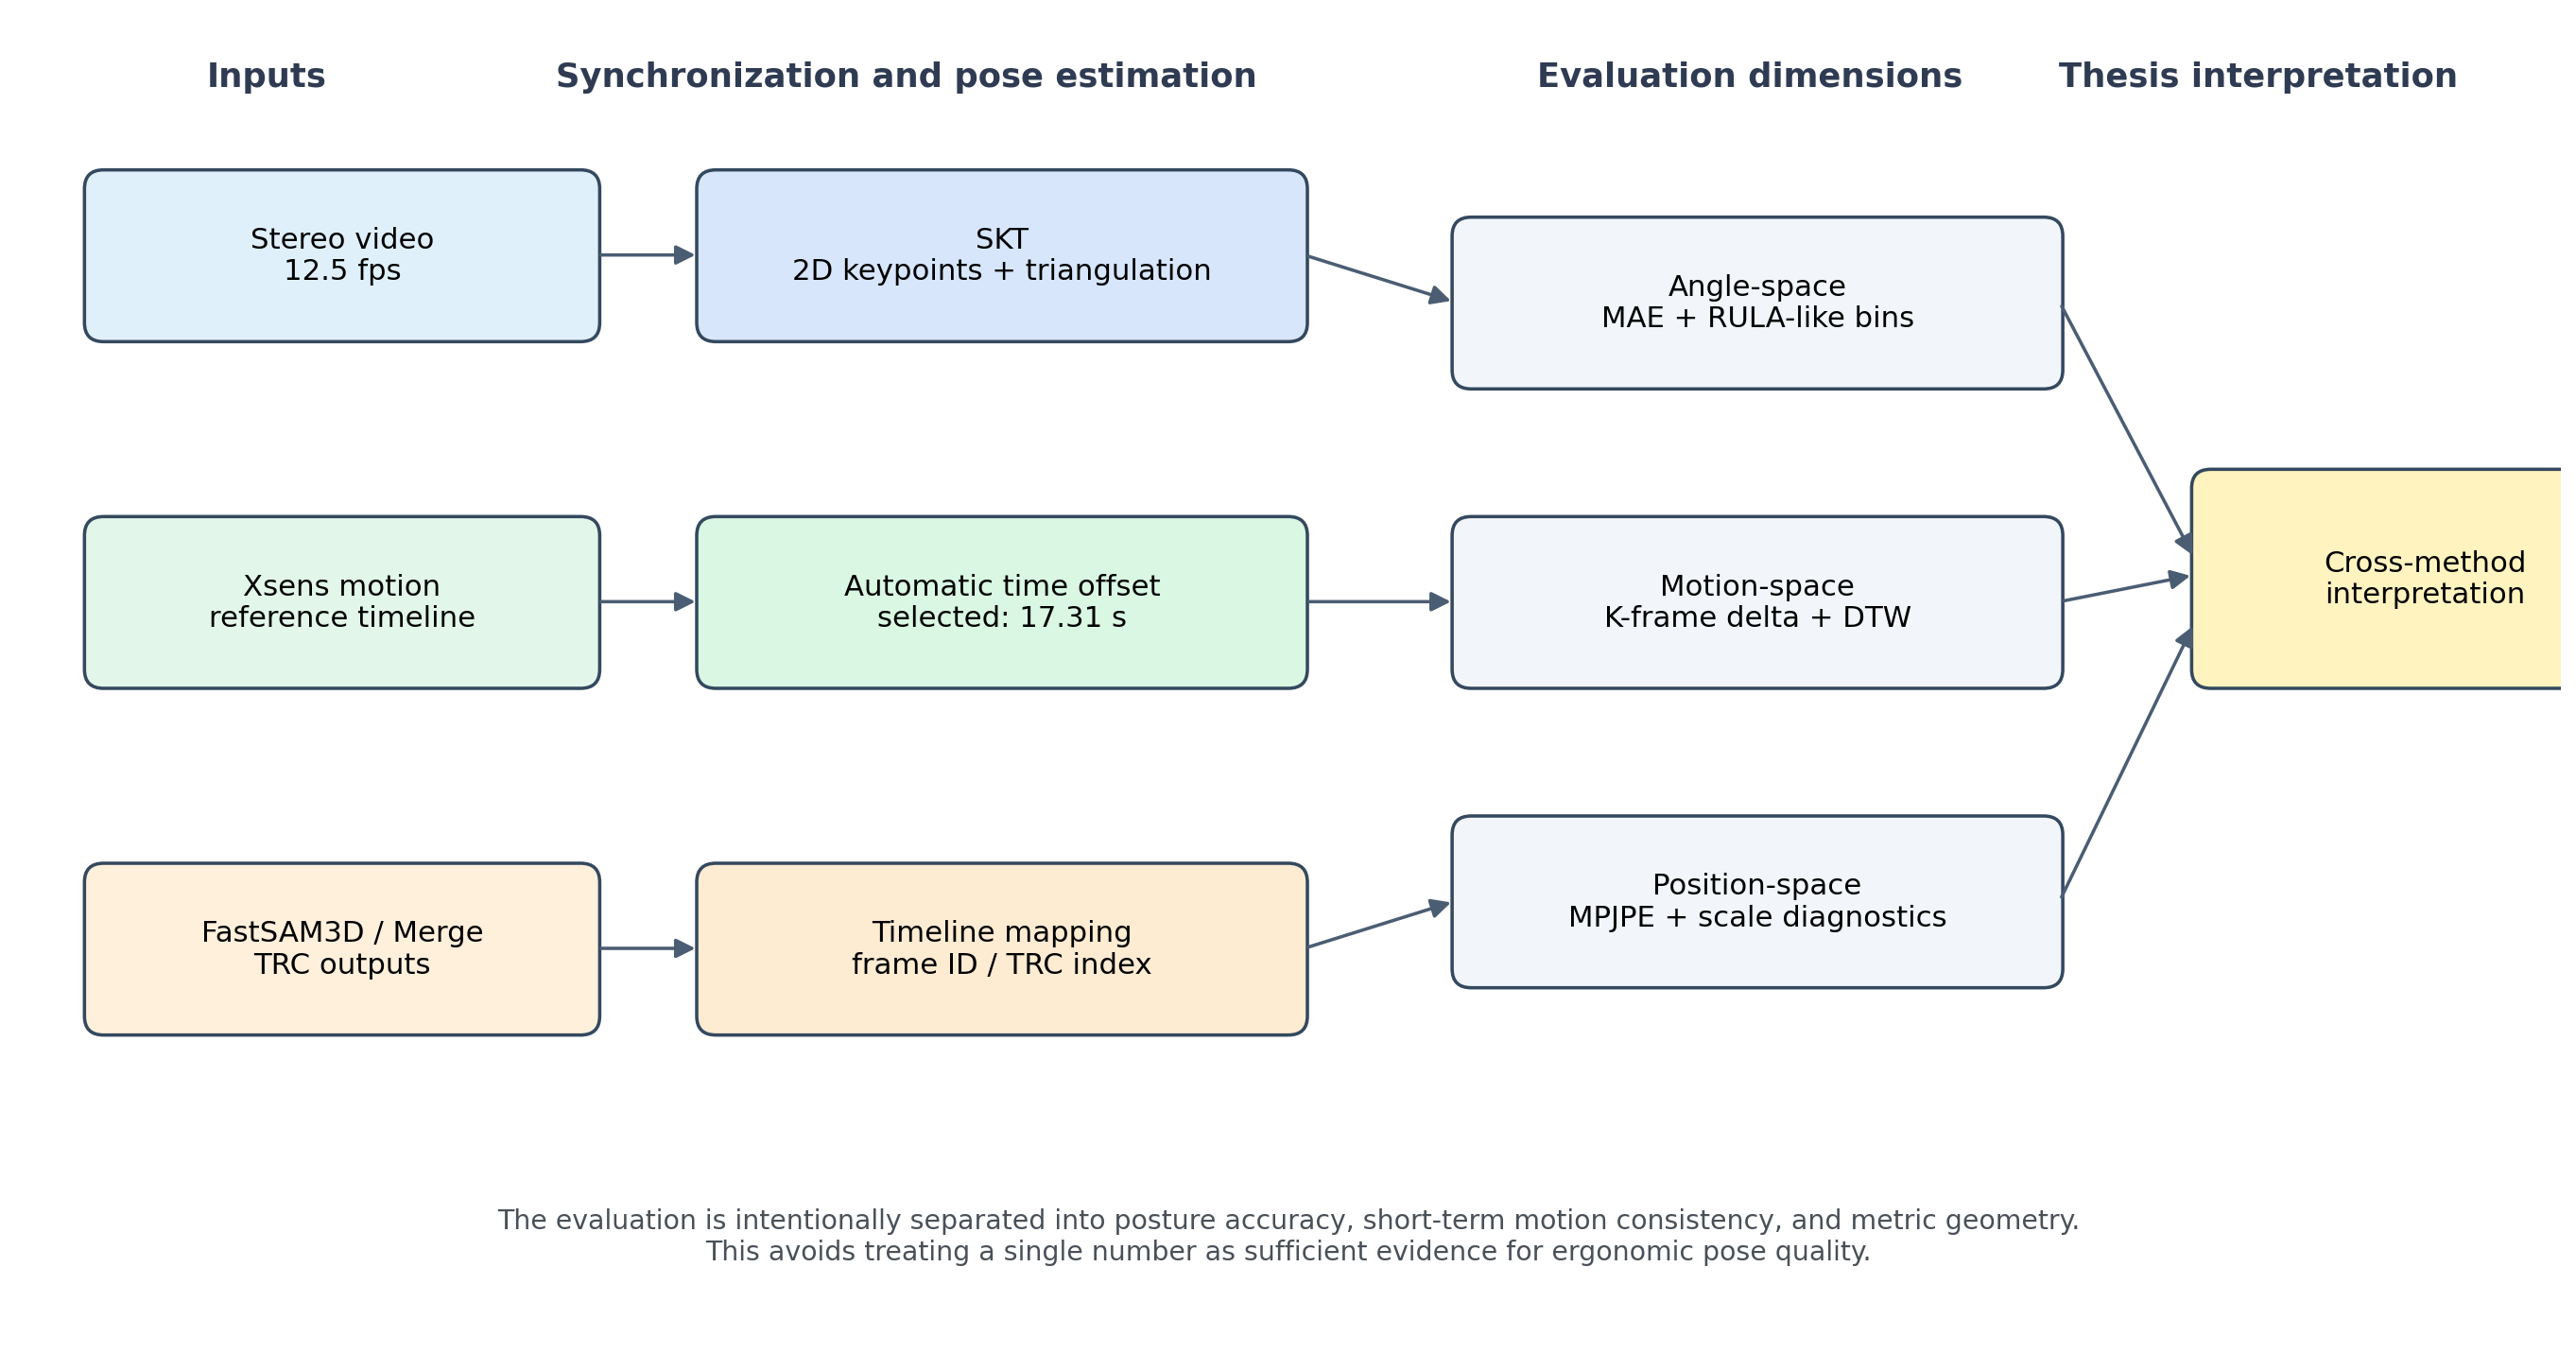
\includegraphics[width=\linewidth]{thesis_pipeline_overview.png}
  \caption{Overview of the thesis evaluation pipeline. Inputs are synchronized and evaluated separately in angle space, motion space, and position space before the final cross-method interpretation.}
  \label{fig:pipeline_overview}
\end{figure}

\begin{table}[!htbp]
  \centering
  \caption{Role of each evaluated pose-estimation path in the thesis.}
  \label{tab:method_roles}
  \small
  \begin{tabularx}{\linewidth}{lXXX}
    \toprule
    Method & Input assumption & Main advantage & Main risk \\
    \midrule
    SKT
    & Synchronized stereo video and calibrated cameras
    & Metric 3D scale and explicit geometric quality signals
    & 2D keypoint jitter and left--right mismatch are amplified by triangulation \\
    FastSAM3D
    & Monocular pose output provided as TRC markers
    & Learned body/motion priors give stable angle and motion behaviour
    & Coordinate, scale, and keypoint semantics require careful interpretation \\
    \bottomrule
  \end{tabularx}
\end{table}

\subsection{Sparse Keypoint Triangulation (SKT)}

The primary method developed in this thesis, Sparse Keypoint Triangulation
(SKT), turns a calibrated stereo video pair into a 3D body skeleton through
a transparent geometric chain that exposes per-frame quality signals at
every stage.
For each synchronised left/right frame pair, the pipeline first runs a 2D
human pose detector on each view to obtain 17 COCO-format keypoints with
per-keypoint confidence; the two views' keypoints are then matched by
keypoint index and filtered by three geometric consistency checks
(minimum triangulation confidence, maximum epipolar error, maximum
reprojection error after triangulation); the surviving pairs are
triangulated into 3D coordinates through the Direct Linear Transform
applied to the calibrated projection matrices; and finally the joint
angles are computed from triplets of 3D keypoints using the same
three-point arccosine formula that is applied to the Xsens-derived
geometric reference.

The methodological reason for building SKT this way -- rather than, for
example, regressing 3D pose directly with a learned model -- is
interpretability under deployment.
Every 3D point in an SKT output is tied to two observed 2D detections and
to a known stereo calibration model, so the pipeline can expose a set of
geometry-aware quality signals (triangulation confidence, epipolar error,
reprojection error, disparity) that downstream ergonomic monitoring can
use as a per-frame trust score; unreliable frames can therefore be
detected and gated rather than silently converted into ergonomic risk
scores, which is a property no end-to-end learned regressor offers for
free.
The corresponding methodological cost is that each SKT 3D point inherits
the noise of its 2D detections in both views; small 2D jitter is first
amplified by triangulation and then further amplified by joint-angle
computation, so SKT is most usefully understood as a measurement pipeline
whose output should be read together with its quality signals rather than
as a smoothed motion sequence.

This view of SKT as a measurement pipeline -- rather than a black-box
reconstruction module -- is also what motivates the later motion-delta
evaluation.
When a wrist or elbow keypoint is detected inconsistently between the two
views, the resulting 3D joint can remain numerically valid (the rays still
intersect, the reprojection is still small) while producing a sharply
different triangulated angle from the surrounding frames, which appears in
later analysis as occasional large motion deltas concentrated near
elbow-chain instabilities.
Section~\ref{sec:discussion} returns to these high-delta cases as concrete
failure evidence rather than treating them as generic noise.

\subsection{FastSAM3D (Monocular Learning Baseline)}

FastSAM3D is included as the learning-based monocular counterpart to SKT
and is the most informative single comparison in the thesis, because it
keeps the same input modality (the camera) but replaces multi-view
geometry with learned body-shape and motion priors.
Instead of triangulating left/right keypoint pairs, FastSAM3D produces a
3D pose directly from one camera stream through a model-based pipeline
that combines fast instance segmentation with learned body-shape and pose
priors \cite{yang2026fastsam3d}; the specific FastSAM3D
implementation is treated here as an externally produced output, and its
results are delivered as TRC marker files that are re-mapped to the
COCO-17 keypoint convention and resampled onto the shared camera timeline
before any evaluation metric is computed.

The methodological reason to include FastSAM3D is that learned body-shape
and motion priors should, in principle, smooth out the per-frame keypoint
noise that hurts SKT, because the learned model implicitly enforces
anatomically consistent transitions between consecutive poses even without
explicit multi-view evidence.
The corresponding methodological cost is that the FastSAM3D output does
not necessarily share the SKT coordinate frame, scale convention, or
exact keypoint semantics; FastSAM3D is therefore evaluated primarily in
the angle and motion axes, where these conventions cancel, while
position-space results are reported only as coordinate/scale diagnostics
rather than as direct pose-quality scores.

\clearpage
% =============================================================
\section{Evaluation Framework}
\label{sec:evaluation}
% =============================================================

\subsection{Angle-space Evaluation}

The angle-space track answers the most direct question for ergonomic
deployment -- ``Is the estimated joint posture quantitatively close to
the reference?'' -- and it is therefore reported first in every per-method
analysis even though it is the axis most exposed to the Xsens calibration
limitation discussed in Section~\ref{sec:background}.
Eight full-body angles are evaluated, covering the four bilateral joints
that drive most of the RULA assessment: left and right shoulder, elbow,
hip, and knee flexion.
To remove angle-definition mismatch between systems, every angle is
computed from the same three-point geometric formula applied to the
relevant triplet of 3D keypoints, both for the vision methods and for the
Xsens-derived geometric reference:
\begin{equation}
  \theta = \arccos\!\left(
    \frac{(\mathbf{p}_A-\mathbf{p}_B)\cdot(\mathbf{p}_C-\mathbf{p}_B)}
         {\|\mathbf{p}_A-\mathbf{p}_B\|\;\|\mathbf{p}_C-\mathbf{p}_B\|}
  \right).
\end{equation}
The main reported metrics are mean absolute error (MAE), median absolute
error, bias (signed mean error), valid-pair ratio, and -- as the
application-level companion -- RULA-like bin agreement for the
upper-body joints.

\subsection{Motion-space Evaluation}

The motion-space track is the thesis's principal countermeasure against
the Xsens calibration offset: it asks whether two systems describe the
\emph{same change in posture} rather than the same absolute posture, so
that any static reference offset cancels out by differencing.
For a given time scale $K$, the K-frame angle delta is defined as
\begin{equation}
  \Delta_K \theta_t \;=\; \theta_t \;-\; \theta_{t-K},
\end{equation}
and the thesis evaluates four time scales, $K\in\{1,6,12,25\}$ frames
(approximately 0.08, 0.48, 0.96, and 2.00\,s at 12.5\,fps), to probe the
agreement across genuinely instantaneous changes, sub-second sub-actions,
1\,s smooth-motion windows, and 2\,s near-action-level windows.
K=6 is adopted as the main reporting and visualisation scale because it
corresponds to a $\sim$0.48\,s sub-action -- short enough to remain a
true motion-level metric, long enough to suppress per-frame keypoint
jitter -- while the K=1 and K=25 numbers provide context as the
noise-dominated and amplitude-dominated extremes.
Reported metrics include Pearson correlation, Spearman rank correlation,
delta MAE and RMSE, high-delta count, and the path ratio (cumulative
absolute target delta divided by cumulative absolute reference delta),
which together separate ``shape agreement'' from ``amplitude agreement''
in the motion signal.

\subsection{Segment-level Evaluation}

The segment-level track condenses the frame-level motion comparison into
a small set of physically interpretable active-movement intervals,
because reporting only frame-level metrics tends to hide whether a method
captures the actual movement bursts that ergonomic risk assessment cares
about.
Activity segments are detected from the reference signal as contiguous
intervals of sustained K-frame motion above a threshold, and for each
segment four numbers are reported per method: range of motion (ROM,
max-min angle), per-segment angle MAE, RULA-like bin agreement based on
the segment's peak angle, and a dynamic time warping (DTW) distance
\cite{sakoe1978dtw}.
The DTW comparison is run on \emph{mean-subtracted and L2-normalised}
per-segment angle sequences, following the practice that has been
recommended for human-motion shape comparison in the recent literature
\cite{perezluque2026reaching}; the normalisation deliberately removes
absolute offset and amplitude so that DTW measures whether the
\emph{shape of motion through the segment} is similar, making it
complementary to MAE/RMSE (which measure amplitude error) rather than
redundant with them.

\subsection{Position-space Evaluation}

The position-space track does not compete with the angle and motion
tracks for ``best pose method'' -- it answers a separate deployment
question: ``Which method produces 3D coordinates whose scale and
geometry can be trusted in a metric workspace?''
For SKT, calibrated stereo geometry gives the coordinates an inherent
metric scale, so MPJPE-style distances and pelvis-relative comparisons
can be reported directly after rigid alignment using the standard Kabsch
estimator \cite{kabsch1976solution}.
For FastSAM3D, the output coordinate frame and scale convention do not
necessarily match the stereo or Xsens frames, so position-space numbers
must be reported with explicit alignment provenance; the thesis uses
position-space results primarily to (i) demonstrate stereo's
metric-scale advantage and (ii) document the coordinate/scale work that
any monocular pipeline must do before its 3D output becomes deployable.

\subsection{Filtering Policy}

The evaluation tracks above are well-defined only if the per-system
filtering policy is itself controlled, because temporal smoothing
applied at different strengths to different systems can quietly inflate
or deflate motion-space agreement without changing any reported number
in an obvious way.
The thesis therefore adopts a deliberate per-system policy.
Xsens streams are interpolated onto the shared timeline but are
\emph{not} re-smoothed by the project, because the Xsens internal
processing already includes substantial filtering, and stacking a
project-side filter on top would silently double the smoothing on
the reference side of every comparison.
The camera-based methods are smoothed with a single light moving-average
filter whose window is recorded in the run configuration; the chosen
window represents a $\sim$200\,ms low-lag setting consistent with empirical
guidance for human upper-body motion signals \cite{perezluque2026reaching}.
The single methodological invariant that must hold across all runs is
that smoothing is always applied \emph{before} delta computation, since
the opposite order would let the delta metric measure filter artifacts
rather than the underlying motion signal.

\begin{table}[!htbp]
  \centering
  \caption{Interpretation of the evaluation tracks used in the thesis.}
  \label{tab:evaluation_tracks}
  \small
  \begin{tabularx}{\linewidth}{lXXX}
    \toprule
    Track & Question answered & Main metrics & Main caveat \\
    \midrule
    Angle-space
    & Is the posture suitable for ergonomic angle interpretation?
    & MAE, median AE, bias, valid ratio, RULA-like bin agreement
    & Sensitive to reference-system angle definitions and static offsets \\
    Motion-space
    & Do two systems describe the same short-term movement?
    & K-frame delta correlation, delta MAE, RMSE, high-delta count, DTW
    & Requires careful time alignment and consistent smoothing policy \\
    Segment-level
    & Are active movement intervals similar in range and shape?
    & ROM error, segment MAE, DTW distance, RULA-like agreement
    & Depends on segment detection thresholds and valid-frame coverage \\
    Position-space
    & Are reconstructed 3D skeletons geometrically compatible?
    & MPJPE, pelvis-relative distance, aligned inter-method distance
    & Monocular methods may use different coordinate and scale conventions \\
    \bottomrule
  \end{tabularx}
\end{table}

This separation is central to the thesis argument.
For example, a method can produce good angle trends while still being
difficult to compare in absolute 3D coordinates, or it can preserve metric
scale while producing jittery short-term angles.
The evaluation framework therefore reports multiple complementary quantities
instead of selecting a single ``winner'' metric.

\clearpage
% =============================================================
\section{Results}
\label{sec:results}
% =============================================================

\subsection{Angle-space Results}

In the angle-space track, the monocular learning-based FastSAM3D pipeline
outperforms SKT, but the margin is small enough that the result must be
read with the Xsens reference-system caveat in mind rather than as a
universal verdict.
Averaged across the eight evaluated joint angles, FastSAM3D reaches a mean
MAE of 15.4\degr\ against the Xsens-derived reference, compared with
17.6\degr\ for SKT; the corresponding median MAEs (14.4\degr\ vs.\
17.9\degr) preserve the same ranking, and FastSAM3D also has the higher
valid-pair ratio (0.905 vs.\ 0.746).
The Xsens-native check sits at 4.7\degr\ MAE, an order of magnitude below
the vision methods, and is reported in the same table only as a
reference-system internal anchor rather than as a competing pose method.

The most informative joint-level pattern is that the per-joint MAE
ranking is not flat across the eight angles.
Shoulder, hip, and knee angles dominate FastSAM3D's lead, where its
learned body priors stabilise the chain endpoints; the elbow is the
hardest joint for every vision method, in line with the long
shoulder--elbow--wrist chain that amplifies both keypoint noise (for SKT)
and pose-prior uncertainty (for FastSAM3D), and this is the joint where
both methods are penalised most by the Xsens calibration offset
itself.
For this reason the elbow is the joint that drives the motion-space
analysis that follows -- angle MAE alone cannot tell which fraction of
the elbow error is genuine pose error and which fraction is reference
offset.

\begin{table}[!htbp]
  \centering
  \caption{Angle-space summary across eight evaluated joint angles. Lower MAE is better.}
  \label{tab:angle_summary}
  \small
  \begin{tabular}{lcccc}
    \toprule
    Method & Mean MAE $\downarrow$ & Median MAE $\downarrow$ &
    Valid ratio $\uparrow$ & Bin agreement $\uparrow$ \\
    \midrule
    SKT & 17.6 & 17.9 & 0.746 & 0.540 \\
    \good{FastSAM3D} & \good{15.4} & \good{14.4} & \good{0.905} & \good{0.553} \\
    \textit{Xsens native check} & \textit{4.7} & \textit{3.7} & \textit{0.905} & \textit{0.886} \\
    \bottomrule
  \end{tabular}
\end{table}

Figure~\ref{fig:angle_summary_plot} visualises the same comparison.
The bar plot is included precisely because the FastSAM3D--SKT gap is
small and consistent rather than large and dramatic; a single bar
that was twice as high as another would not survive any reasonable
sensitivity check on this single recording, whereas a small but
systematic gap is the more honest evidence on which to base the
discussion of learned pose priors later in the thesis.

\begin{figure}[!htbp]
  \centering
  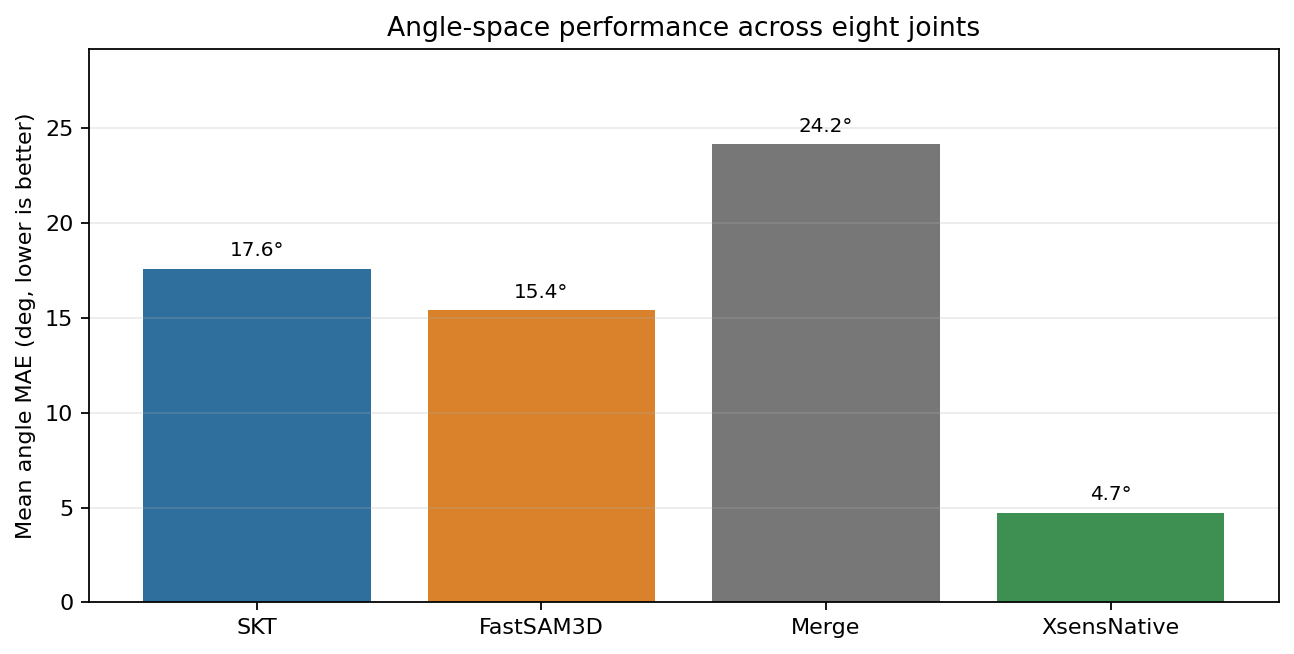
\includegraphics[width=0.92\linewidth]{thesis_angle_summary.png}
  \caption{Angle-space summary across evaluated methods. FastSAM3D has the lowest mean and median MAE among the vision methods, while the Xsens-native check indicates the approximate lower bound of the reference-system representation difference.}
  \label{fig:angle_summary_plot}
\end{figure}

\subsection{Motion-space Results}

In the motion-space track, the FastSAM3D advantage observed in absolute
angles becomes both clearer and easier to interpret, because differencing
the angle sequences cancels the Xsens calibration offset that confounded
the angle-space comparison.
Averaged across the eight evaluated angles at $K=6$ frames ($\sim$0.48\,s),
FastSAM3D reaches a mean Pearson correlation of 0.64 with the Xsens-derived
reference, against 0.38 for SKT; the corresponding mean Spearman rank
correlations (0.64 vs.\ 0.33) preserve the same ranking, which rules out
the explanation that FastSAM3D is winning only because of a handful of
high-amplitude points that inflate Pearson without lifting the rank
correlation.
At the elbow -- the joint that the motion-space track is designed to
adjudicate -- FastSAM3D reaches Pearson correlations of 0.54 (left) and
0.69 (right) against SKT's 0.39 / 0.39, a comparable shape-agreement gap
on the joint that the angle-space analysis flagged as ambiguous.
The Xsens-native check returns the expected $\sim$0.96 mean correlation,
confirming that the K=6 metric can recover near-perfect agreement when
the two compared signals genuinely measure the same motion.

\begin{table}[!htbp]
  \centering
  \caption{K=6 motion-delta agreement. Higher correlation is better.}
  \label{tab:motion_summary}
  \small
  \begin{tabular}{lcccc}
    \toprule
    Method & Mean $r$ $\uparrow$ & Mean $\rho$ $\uparrow$ &
    L-elbow $r$ $\uparrow$ & R-elbow $r$ $\uparrow$ \\
    \midrule
    SKT & 0.379 & 0.334 & 0.392 & 0.386 \\
    \good{FastSAM3D} & \good{0.644} & \good{0.635} & \good{0.542} & \good{0.689} \\
    \textit{Xsens native check} & \textit{0.965} & \textit{0.936} & \textit{0.988} & \textit{0.993} \\
    \bottomrule
  \end{tabular}
\end{table}

Figure~\ref{fig:motion_k6_summary_plot} visualises the K=6 correlation
summary and makes the main finding immediately legible: FastSAM3D is
consistently above SKT across the eight evaluated angles, and the Xsens-native
check provides the visual upper bound that anchors the scale of the plot.
The per-elbow scatter plots in Figure~\ref{fig:k6_elbow_scatter} then make
the same comparison at the frame level rather than the summary level:
FastSAM3D's scatter clusters along the ideal diagonal with limited vertical
spread, whereas SKT's scatter shows a recurring vertical accumulation near
zero reference delta -- the geometric signature of high SKT delta values
during physically quiet intervals, which Section~\ref{sec:discussion}
traces back to localised keypoint-chain instability rather than to a
constant noise floor.

\begin{figure}[!htbp]
  \centering
  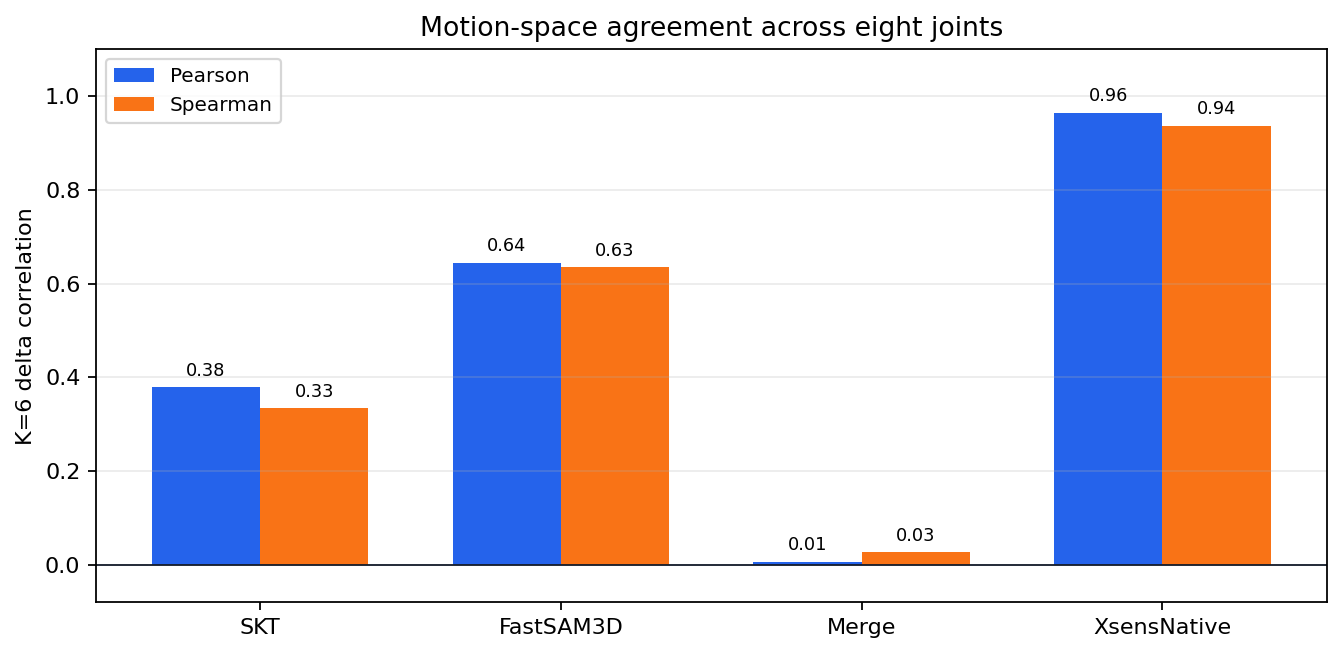
\includegraphics[width=0.92\linewidth]{thesis_motion_k6_summary.png}
  \caption{K=6 motion-delta correlation summary. FastSAM3D shows stronger short-term motion agreement than SKT on the current dataset.}
  \label{fig:motion_k6_summary_plot}
\end{figure}

\begin{figure}[!htbp]
  \centering
  \begin{subfigure}[b]{0.48\linewidth}
    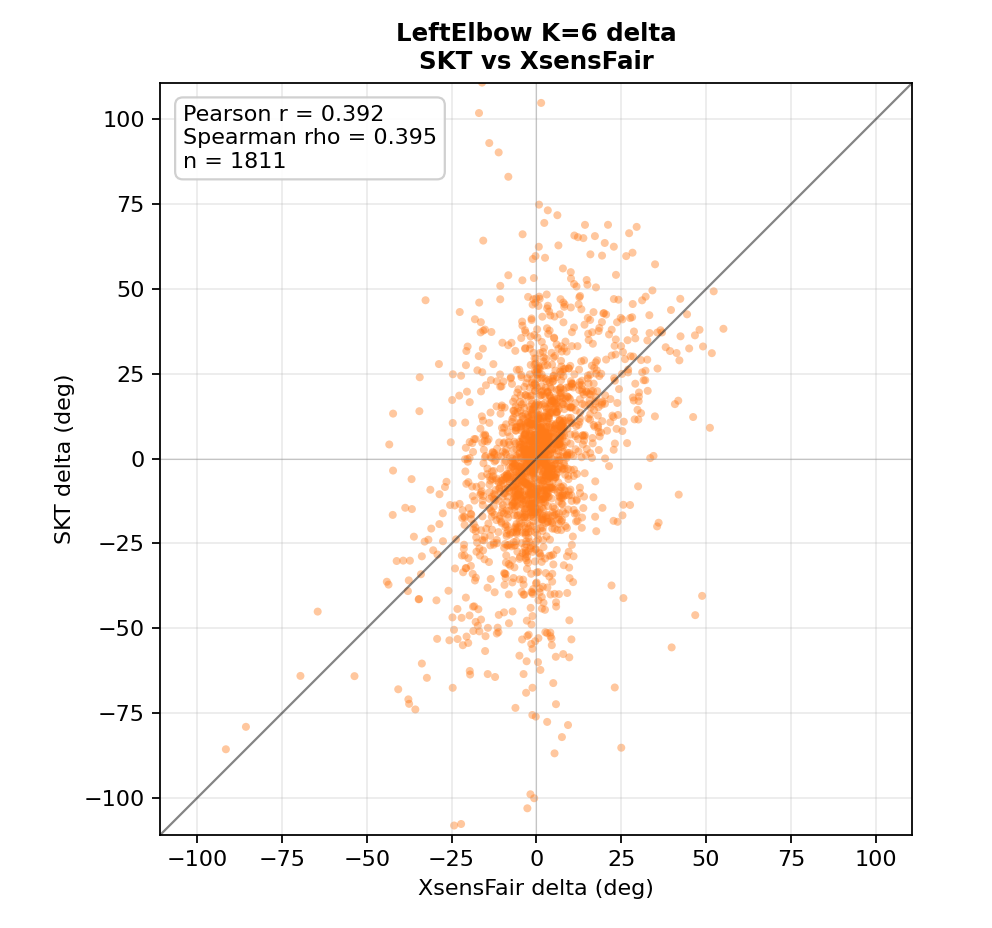
\includegraphics[width=\linewidth]{thesis_scatter_skt_vs_xsensfair_leftelbow_k6.png}
    \caption{SKT, left elbow.}
  \end{subfigure}
  \hfill
  \begin{subfigure}[b]{0.48\linewidth}
    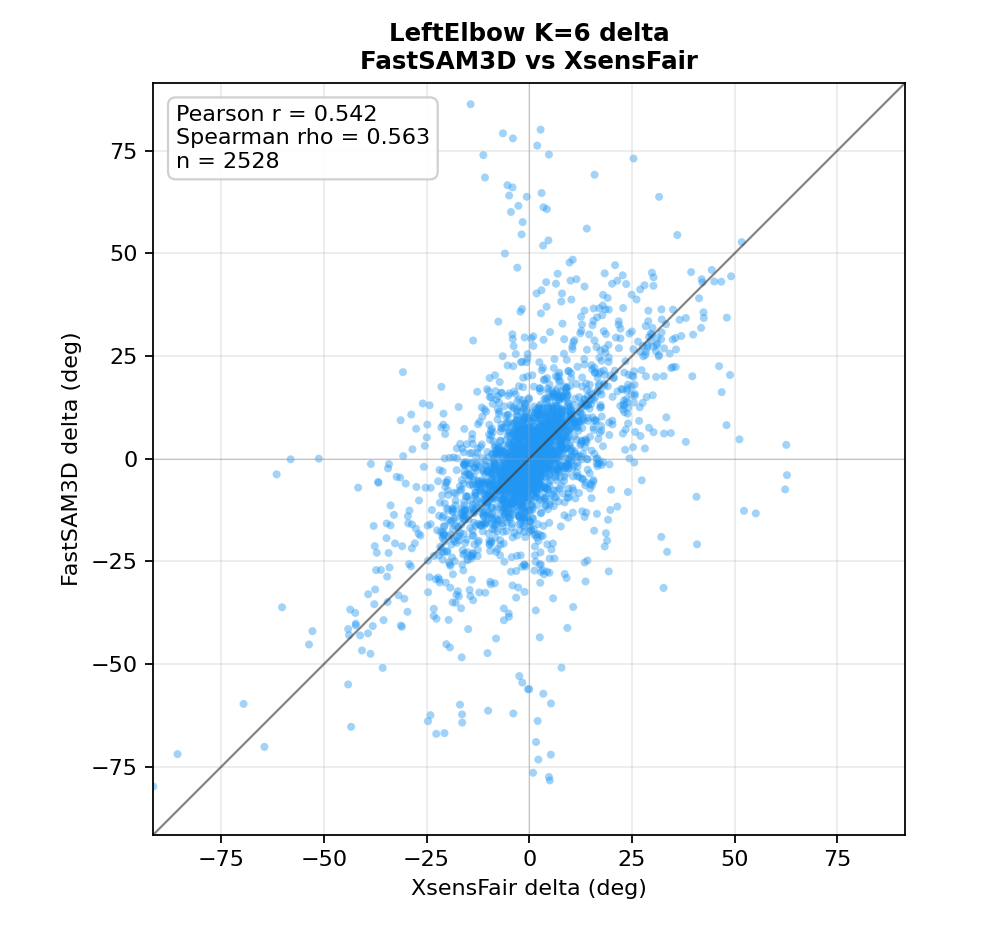
\includegraphics[width=\linewidth]{thesis_scatter_fastsam3d_vs_xsensfair_leftelbow_k6.png}
    \caption{FastSAM3D, left elbow.}
  \end{subfigure}

  \vspace{0.4cm}
  \begin{subfigure}[b]{0.48\linewidth}
    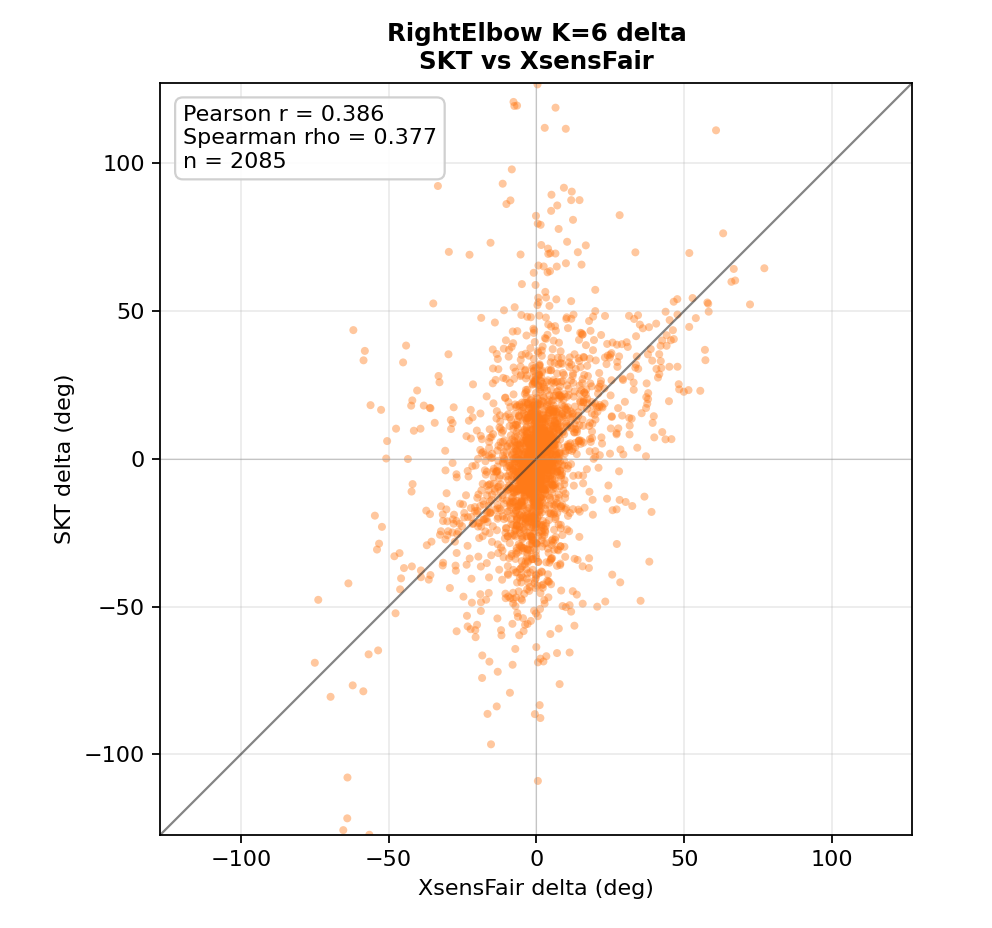
\includegraphics[width=\linewidth]{thesis_scatter_skt_vs_xsensfair_rightelbow_k6.png}
    \caption{SKT, right elbow.}
  \end{subfigure}
  \hfill
  \begin{subfigure}[b]{0.48\linewidth}
    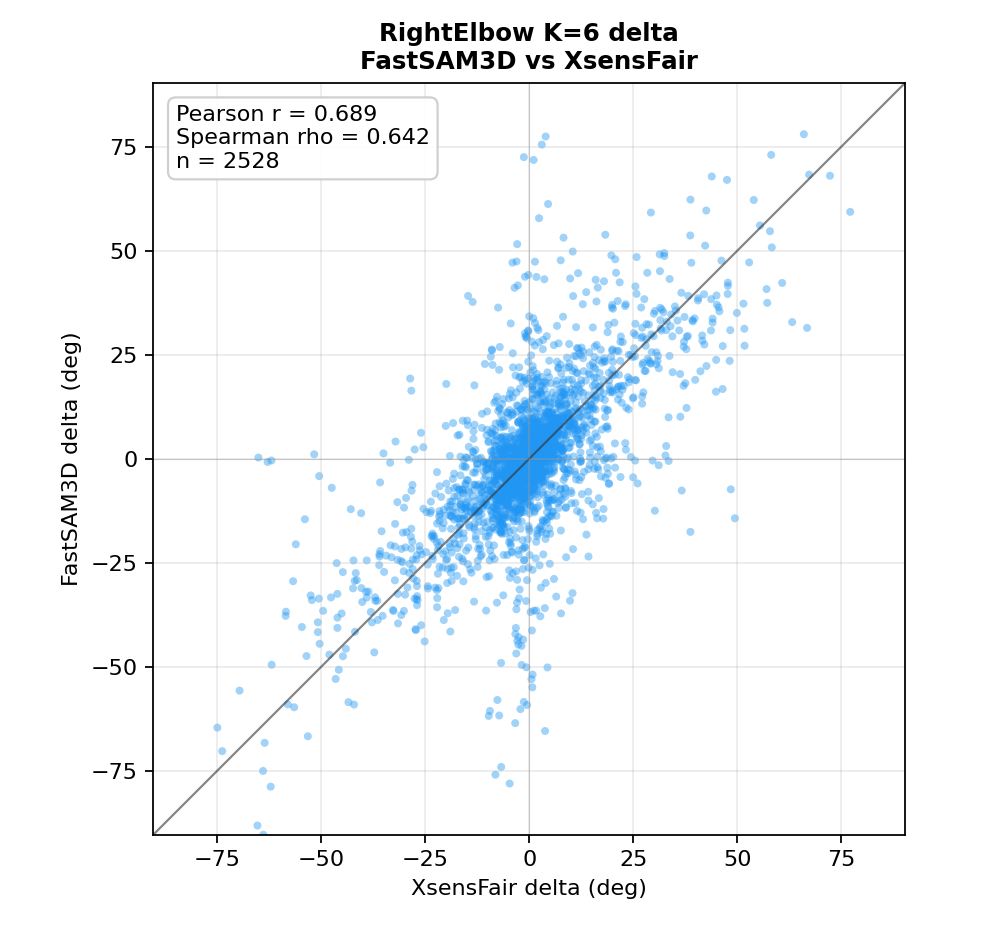
\includegraphics[width=\linewidth]{thesis_scatter_fastsam3d_vs_xsensfair_rightelbow_k6.png}
    \caption{FastSAM3D, right elbow.}
  \end{subfigure}
  \caption{K=6 elbow motion-delta scatter plots against the Xsens-derived reference. FastSAM3D follows the ideal trend more consistently, while SKT shows more high-delta jitter and vertical-axis accumulation.}
  \label{fig:k6_elbow_scatter}
\end{figure}

The sensitivity of the motion-space ranking to the chosen time scale is
shown in Figure~\ref{fig:pearson_vs_k}.
At $K=1$ (single-frame deltas, $\sim$80\,ms) every vision method's
correlation drops because the metric is dominated by per-frame keypoint
jitter that is roughly uncorrelated with the reference; at $K=25$
($\sim$2\,s) every vision method's correlation rises because the metric
is approaching an amplitude-of-motion comparison rather than a true
short-term agreement.
The thesis adopts $K=6$ as the main reporting point because it lies on
the elbow of these two trends: it suppresses single-frame keypoint noise
without smoothing across a complete action, so the ranking it produces
remains a genuine motion-agreement statement rather than either a
noise floor or a re-statement of segment-level ROM.

\begin{figure}[!htbp]
  \centering
  \begin{subfigure}[b]{0.48\linewidth}
    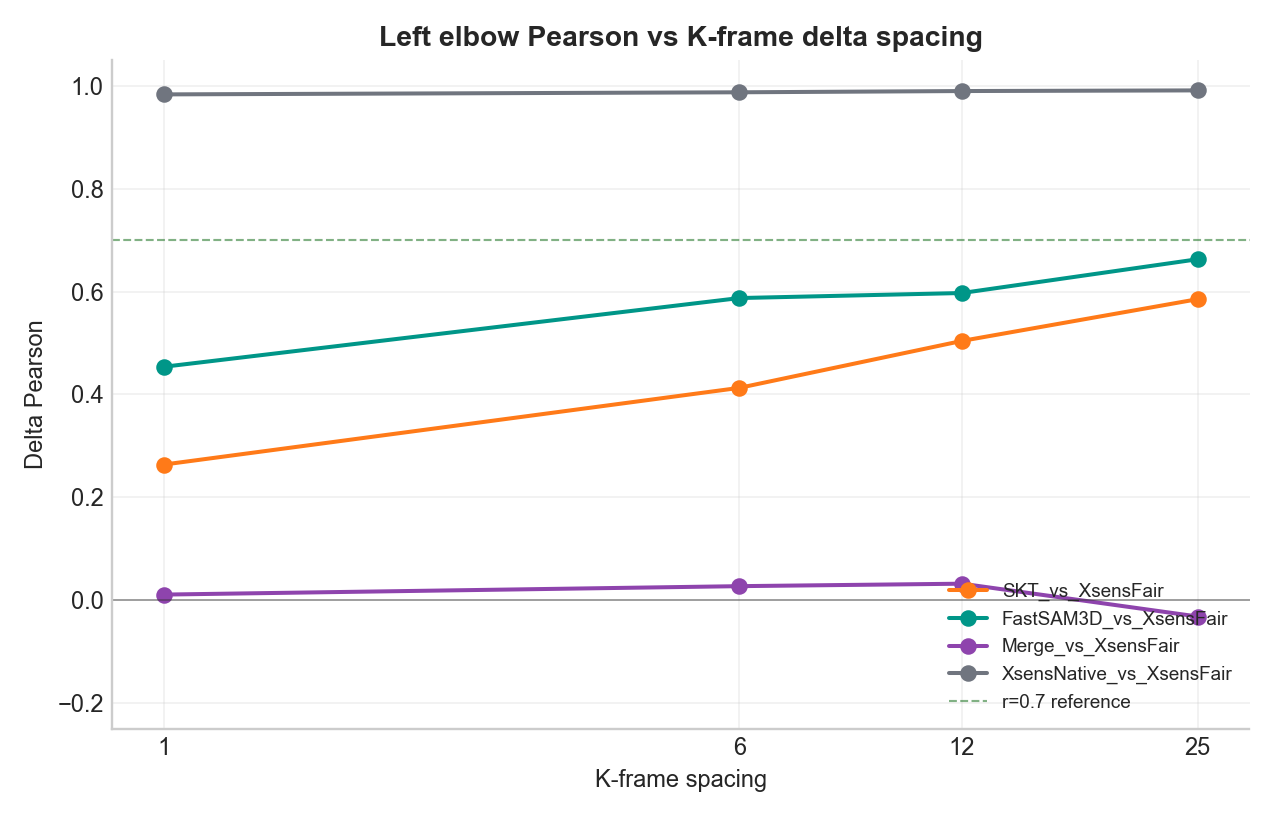
\includegraphics[width=\linewidth]{thesis_pearson_vs_k_leftelbow.png}
    \caption{Left elbow.}
  \end{subfigure}
  \hfill
  \begin{subfigure}[b]{0.48\linewidth}
    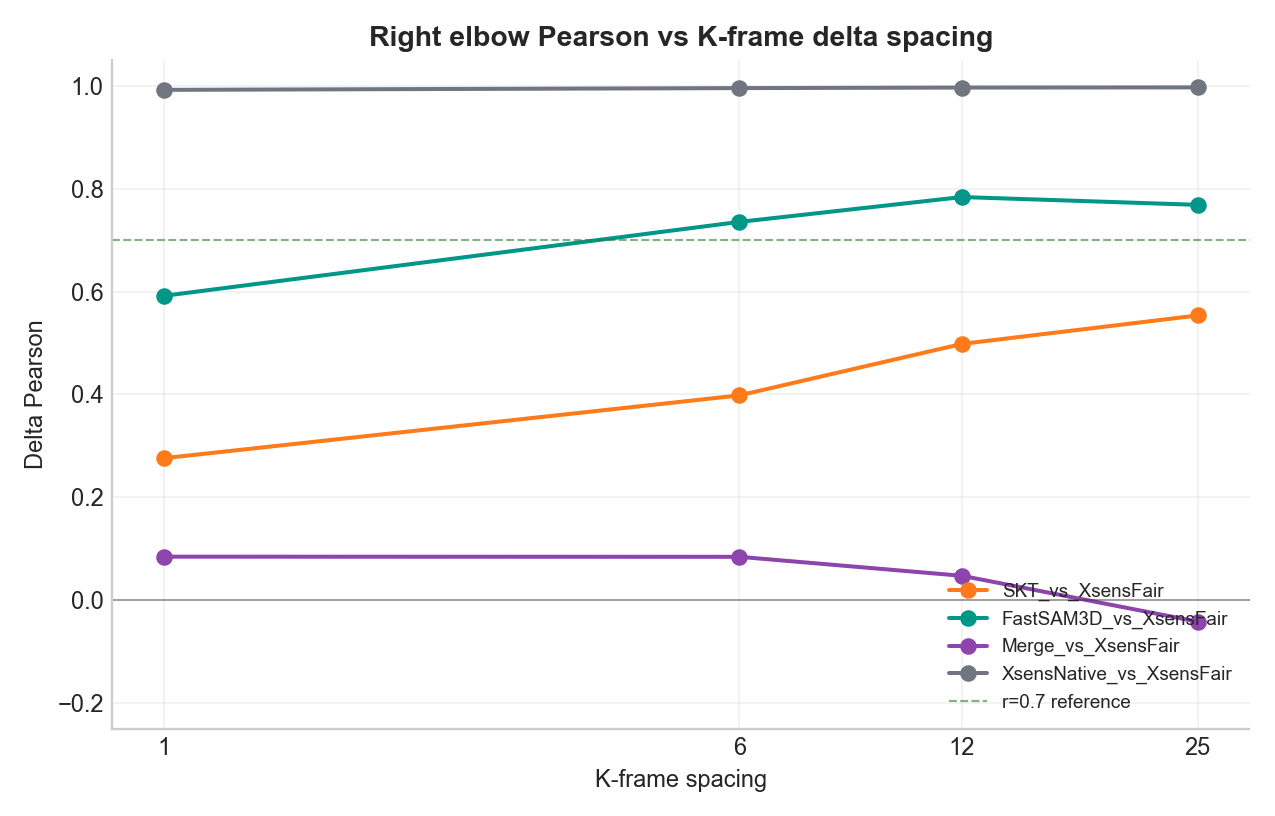
\includegraphics[width=\linewidth]{thesis_pearson_vs_k_rightelbow.png}
    \caption{Right elbow.}
  \end{subfigure}
  \caption{Motion-delta correlation as a function of K. The result supports using K=6 as a practical compromise between jitter sensitivity and motion interpretability.}
  \label{fig:pearson_vs_k}
\end{figure}

\subsection{Segment-level Results}

The segment-level track reinforces the frame-level motion finding while
adding two pieces of information that the frame-level numbers alone cannot
provide: per-segment range-of-motion (ROM) error in degrees, which is the
quantity most directly comparable to a ``movement size'' an ergonomist
would estimate manually, and per-segment normalised DTW distance, which
quantifies how similar the shape of motion through each segment is once
amplitude and offset are removed.
Aggregated over the detected active segments (39 for SKT, 45 for
FastSAM3D), FastSAM3D has both the lower mean ROM error (14.9\degr\ vs.\
26.9\degr\ for SKT) and the lower mean DTW distance (0.0355 vs.\ 0.0435).
The Xsens-native DTW distance ($\sim$6$\times 10^{-3}$) sets the lower
bound that the normalised DTW metric can reach on this dataset, so
FastSAM3D's $\sim$3.5$\times 10^{-2}$ is approximately six times the
reference floor, which is the right order of magnitude to claim
``competitive'' rather than ``saturated''.

\begin{table}[!htbp]
  \centering
  \caption{Segment-level summary over detected active movement intervals. Lower values are better.}
  \label{tab:segment_summary}
  \begin{tabular}{lccc}
    \toprule
    Method & Segments & Mean ROM error (\degr) $\downarrow$ & Mean DTW distance $\downarrow$ \\
    \midrule
    SKT & 39 & 26.9 & 0.0435 \\
    \good{FastSAM3D} & 45 & \good{14.9} & \good{0.0355} \\
    \textit{Xsens native check} & \textit{45} & \textit{4.8} & \textit{0.0062} \\
    \bottomrule
  \end{tabular}
\end{table}

\begin{figure}[!htbp]
  \centering
  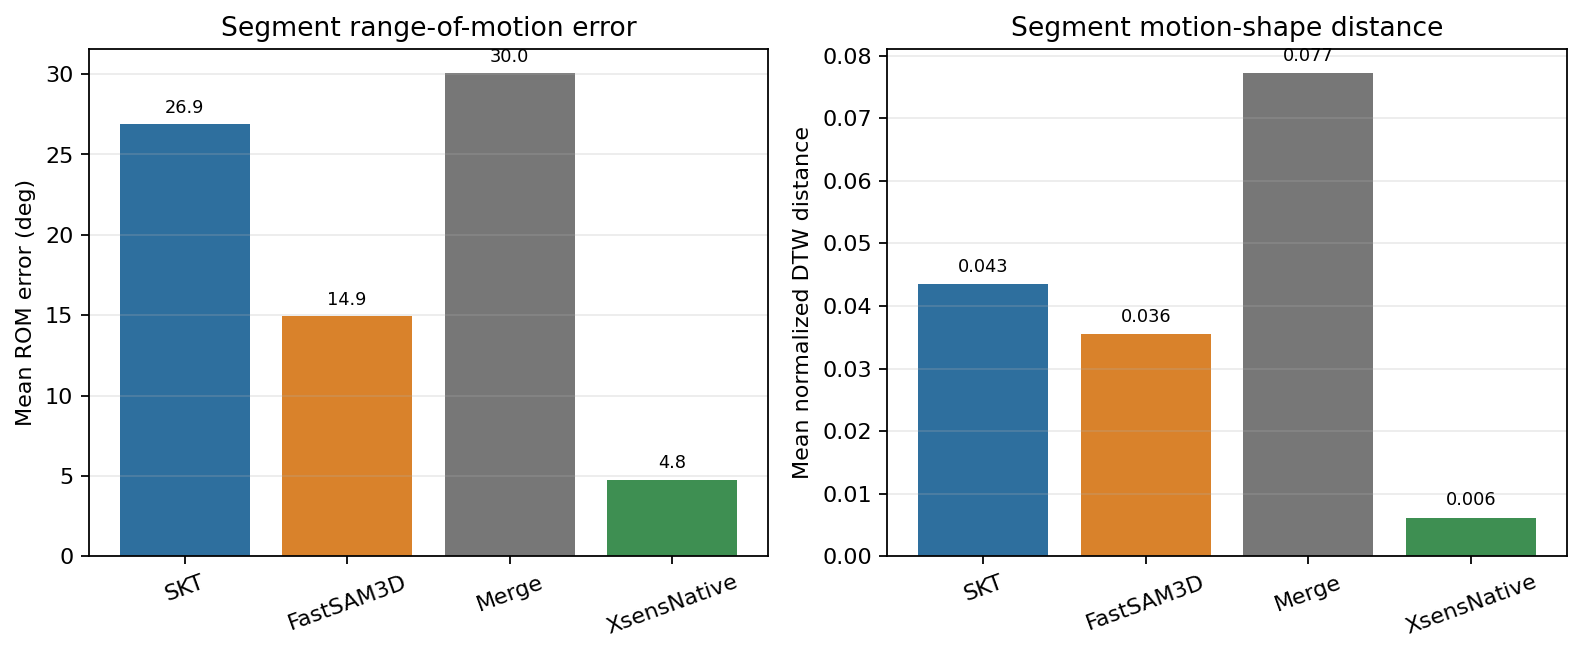
\includegraphics[width=0.95\linewidth]{thesis_segment_summary.png}
  \caption{Segment-level ROM error and DTW distance. FastSAM3D gives the strongest segment-level agreement among the vision methods, while the Xsens-native check provides a reference-system lower bound.}
  \label{fig:segment_summary_plot}
\end{figure}

\subsection{Position-space Results}

The position-space track produces a deliberately different interpretation
from the angle and motion tracks, and reading it as a competing
quality ranking would be a mistake.
SKT recovers 3D coordinates with metric scale inherited from calibrated
stereo geometry, so its distance to the Xsens-derived reference -- 30.6\,cm
mean (20.8\,cm median) after rigid Kabsch alignment -- is a meaningful
geometric quantity whose magnitude can be discussed in the same units as
the workspace itself.
FastSAM3D's direct distance to the Xsens reference under identical
coordinate assumptions is approximately 300\,cm, which is two orders of
magnitude larger; this number, however, does not say that FastSAM3D's
poses are visually two orders of magnitude worse -- it says that the raw
FastSAM3D output uses a different coordinate origin and scale convention,
and the dominant component of the 300\,cm distance is therefore a global
similarity transform that has not yet been resolved.
When FastSAM3D is instead aligned directly to SKT over a set of common
joints, the residual mean distance drops to approximately 60\,cm,
clarifying that the genuine inter-method 3D disagreement is at the
half-metre scale rather than the multi-metre scale and isolating it from
the coordinate-convention issue.

The methodological consequence is reported in
Table~\ref{tab:position_summary} rather than asserted in prose: the
position-space numbers must be read as \emph{coordinate/scale
diagnostics} that document the operational cost of using each method in
metric 3D space, not as another lap of the angle-space ranking
competition.
SKT inherits its metric scale automatically from the calibrated camera
baseline (Section~\ref{sec:data_setup}), so a downstream RULA scorer or
workspace-overlay tool can read its 3D coordinates directly; FastSAM3D
needs a separate scale/coordinate alignment step, which is feasible but
adds operational complexity that this thesis flags explicitly rather
than leaves implicit.

\begin{table}[!htbp]
  \centering
  \caption{Position-space diagnostic results. These values should be interpreted as coordinate/scale diagnostics rather than pure pose-quality rankings.}
  \label{tab:position_summary}
  \small
  \begin{tabularx}{\linewidth}{lccX}
    \toprule
    Comparison & Mean distance & Median distance & Notes \\
    \midrule
    SKT vs.\ reference & 30.6 cm & 20.8 cm & Metric stereo scale after rigid alignment \\
    FastSAM3D vs.\ reference & 300.3 cm & 294.8 cm & Coordinate/scale convention mismatch dominates \\
    FastSAM3D aligned to SKT & 60.0 cm & 36.3 cm & Direct inter-method skeleton comparison \\
    \bottomrule
  \end{tabularx}
\end{table}

\begin{figure}[!htbp]
  \centering
  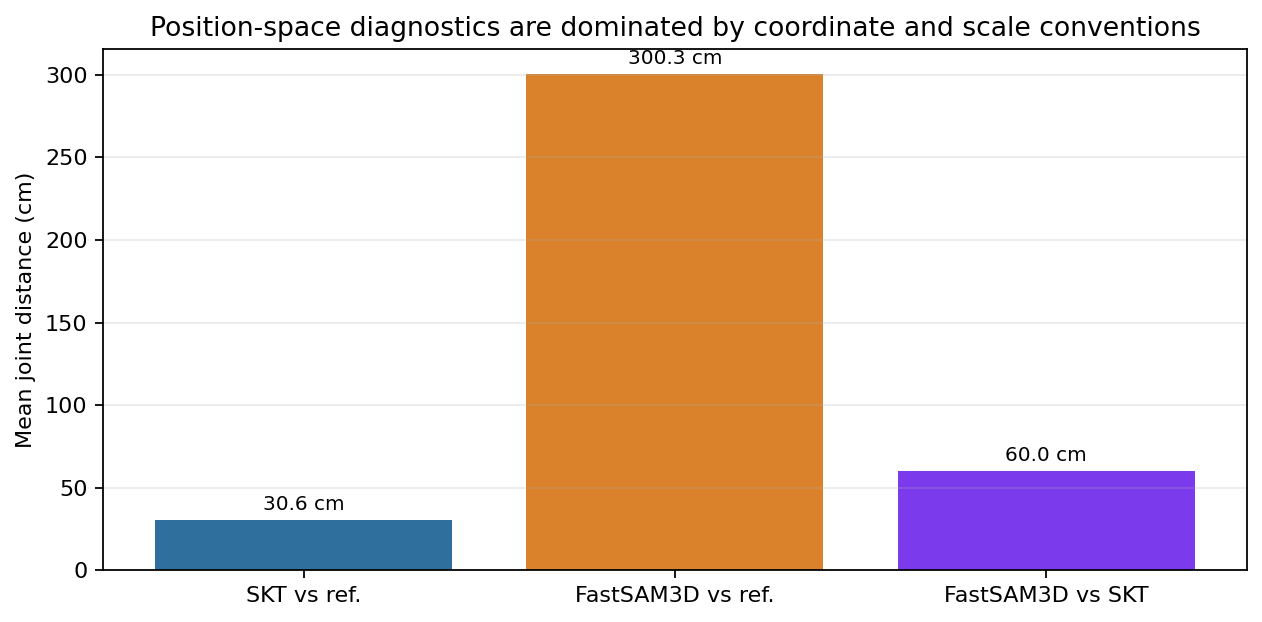
\includegraphics[width=0.9\linewidth]{thesis_position_diagnostic.png}
  \caption{Position-space diagnostic comparison. SKT is more meaningful in metric 3D space because it is tied to calibrated stereo geometry, whereas direct FastSAM3D-to-reference distance is dominated by coordinate and scale conventions.}
  \label{fig:position_diagnostic_plot}
\end{figure}

\subsection{Cross-method Synthesis}

Reading the two evaluation tracks together produces a more complete picture
than either gives on its own.
Table~\ref{tab:cross_method_synthesis} consolidates the headline numbers
for SKT and FastSAM3D (with the Xsens-native check shown alongside as a
reference-system floor).
FastSAM3D leads on the angle-space (lower MAE) and motion-space (higher
correlation) tracks, which together indicate that learned body and motion
priors suppress the per-frame jitter that hurts a frame-independent
sparse stereo reconstruction on this dataset.
SKT lags FastSAM3D on angle and motion but its 3D coordinates carry metric
scale by construction, and the per-frame geometric quality signals it exposes
(epipolar error, reprojection error, triangulation confidence) are exactly
the signals that downstream ergonomic quality gating requires.

\begin{table}[!htbp]
  \centering
  \caption{SKT vs FastSAM3D headline synthesis across evaluation tracks. Best value per column is highlighted; the Xsens-native row is a reference-system internal check, not a competing method.}
  \label{tab:cross_method_synthesis}
  \small
  \begin{tabular}{lccccl}
    \toprule
    Method & Angle MAE (\degr) $\downarrow$ & RULA bin agree.\ $\uparrow$ & Motion $r$ K=6 $\uparrow$ & Segment ROM (\degr) $\downarrow$ & Metric scale \\
    \midrule
    SKT
    & 17.6 & 0.540 & 0.379 & 26.9 & \good{Calibrated} \\
    \good{FastSAM3D}
    & \good{15.4} & \good{0.553} & \good{0.644} & \good{14.9} & Needs alignment \\
    \textit{Xsens native (ref.)}
    & \textit{4.7} & \textit{0.886} & \textit{0.965} & \textit{4.8} & \textit{---} \\
    \bottomrule
  \end{tabular}
\end{table}

The overall pattern is: \emph{the learning-based monocular pipeline wins
the angle and motion agreement tracks; the calibrated stereo pipeline
retains the deployment-geometry advantage; and neither replaces the other.}
This split is the substantive result of the synthesis and is what
Section~\ref{sec:discussion} examines in operational terms.

\clearpage
% =============================================================
\section{Discussion}
\label{sec:discussion}
% =============================================================

\subsection{Why FastSAM3D Performs Better in Angle and Motion Space}

The most likely reason FastSAM3D leads SKT on the angle and motion tracks
is that its learned body-structure and motion-continuity priors mask
exactly the per-frame failure mode that hurts a frame-independent
triangulation pipeline.
FastSAM3D's 3D output for any given frame is conditioned on body-shape
plausibility constraints that were absorbed from large pose-sequence
training corpora, so a momentarily unreliable keypoint produces a
smoothed-out anatomical correction rather than a sharp angle spike; this
is qualitatively visible in the K=6 elbow scatter plots
(Figure~\ref{fig:k6_elbow_scatter}), where the FastSAM3D scatter sits
along the ideal y=x diagonal whereas the SKT scatter shows recurring
vertical accumulation -- large target deltas at small reference deltas --
that no amount of point-density change can hide.
This shape of error matters for the interpretation: the SKT weakness is
not a uniform random noise floor but a structured failure pattern
concentrated on a small fraction of frames, which suggests that targeted
quality-aware repair rather than uniform smoothing is the appropriate
remedy.

\subsection{Why Stereo Geometry Still Matters}

The FastSAM3D advantage on the agreement tracks does not eliminate the
case for calibrated stereo geometry, because deployment in a real
manufacturing setting cares about two properties that the agreement
tracks alone do not test: whether the 3D coordinates are in real metric
units, and whether the system can flag its own unreliable frames before
they reach a downstream ergonomic risk score.
SKT inherits metric scale from the calibrated camera baseline, so its 3D
coordinates can be overlaid on workspace geometry without an additional
alignment step, whereas any monocular learning-based pipeline needs an
explicit external scale and coordinate recovery before its output is
usable in the same role.
More importantly, SKT exposes a per-frame geometric quality vector --
triangulation confidence, epipolar error, reprojection error,
left--right keypoint agreement -- whose individual components are tied
to the camera model, so an automated downstream stage can refuse to
score frames whose quality vector falls outside the working envelope;
an end-to-end learned pipeline can in principle be augmented with
calibrated uncertainty heads, but that augmentation is itself an open
research problem rather than a property the FastSAM3D output exposes
today.

\subsection{Failure-case Analysis of High-delta Events}

The K=6 scatter pattern noted above is not generic noise but a small
number of identifiable keypoint-chain failures, and treating it as
such is what makes the next SKT iteration tractable.
For elbow flexion, the relevant chain is shoulder--elbow--wrist; an
unstable wrist detection in either camera can leave the triangulated
shoulder and elbow correct, satisfy all geometric quality checks
individually, and still produce an elbow angle that jumps by tens of
degrees in a single frame, because the angle depends on the relative
direction of two segments rather than on the absolute position of any
single keypoint.
Figure~\ref{fig:skt_high_delta_cases} shows two representative SKT
high-delta intervals projected back onto the original video; the
problematic frames in each clip share three concrete characteristics --
partial occlusion of the wrist by the body or by an object, large
camera-to-subject distance, and inconsistent left/right detection of
the elbow chain -- rather than appearing at random across the
recording.
The operational implication is that the next SKT improvement should
focus on chain-aware (not single-keypoint-aware) quality filtering
together with short-window temporal repair, since both interventions
target the specific failure mode evidenced here and neither requires
changing the underlying triangulation or angle formula.

\subsection{Applicability Boundaries}

Putting these analyses together gives a concrete recommendation for
when each method type should be preferred in industrial ergonomic
monitoring, rather than a universal ranking statement.
For deployment scenarios that need only joint-angle outputs and short-term
motion signals -- for example a fixed-camera workstation that scores
postures from skeletons but does not need to overlay them on real
geometry -- a learning-based monocular pipeline of the FastSAM3D family
is the more competitive choice on this dataset, both because its
absolute angle MAE is lower and because its short-term motion signal is
visibly more stable.
For deployment scenarios that need metric 3D scale, workspace overlay,
or per-frame quality gating before downstream automated scoring -- which
is the more typical industrial setting -- calibrated stereo remains
the more defensible default, because both the metric coordinates and
the geometric quality signals are properties of the camera model rather
than of the trained model.
The thesis therefore does not recommend one method as universally
correct, and the practical question for any new deployment is which of
these two sets of requirements dominates.

\begin{figure}[!htbp]
  \centering
  \begin{subfigure}[b]{0.98\linewidth}
    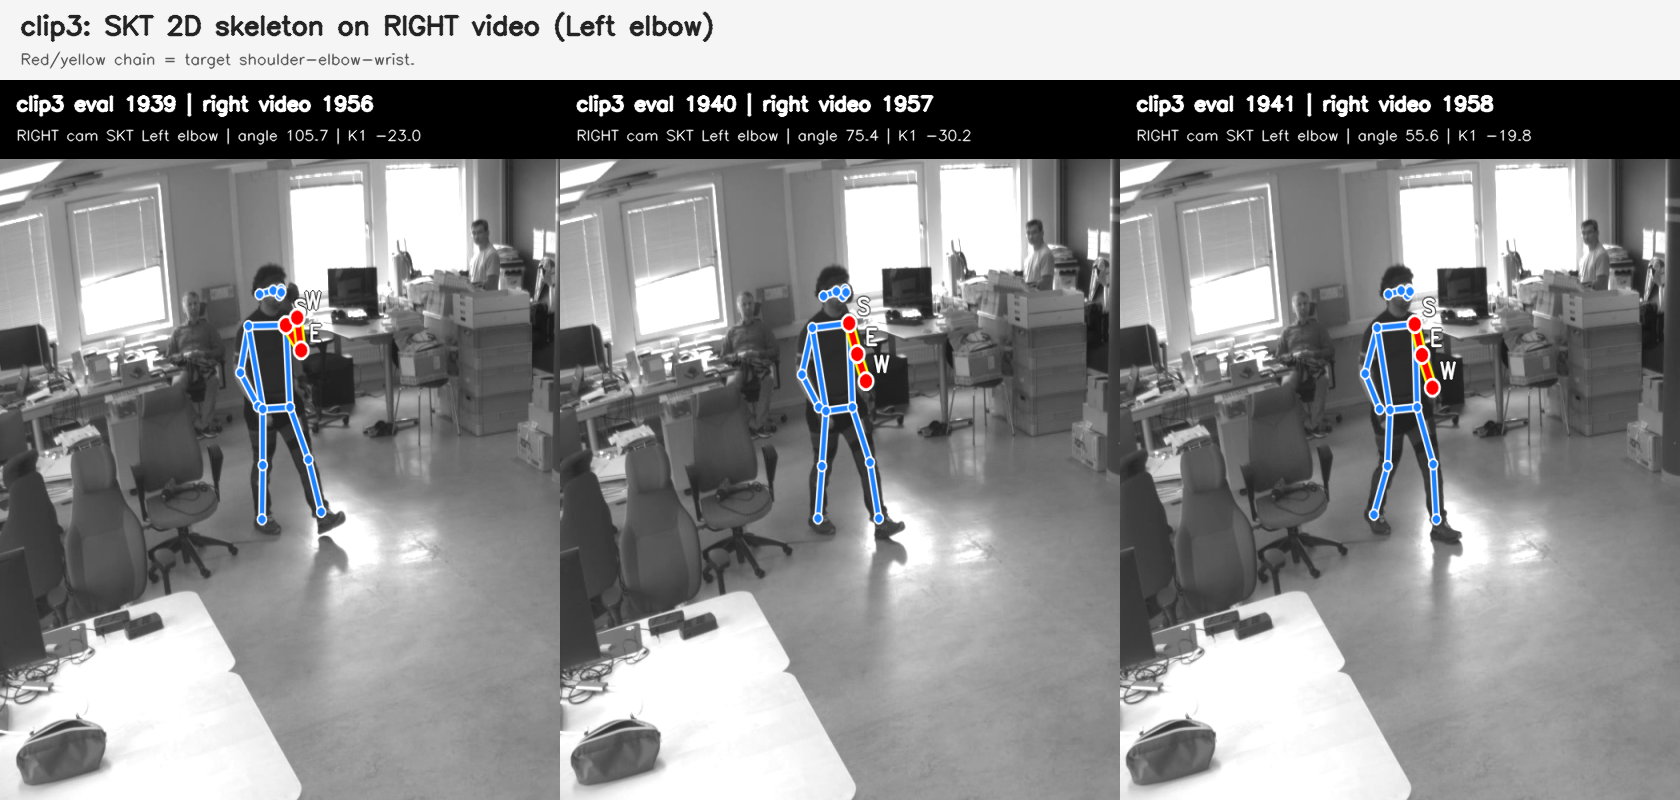
\includegraphics[width=\linewidth]{thesis_skt_high_delta_left_elbow_frames.png}
    \caption{Left-elbow high-delta interval.}
  \end{subfigure}

  \vspace{0.35cm}
  \begin{subfigure}[b]{0.98\linewidth}
    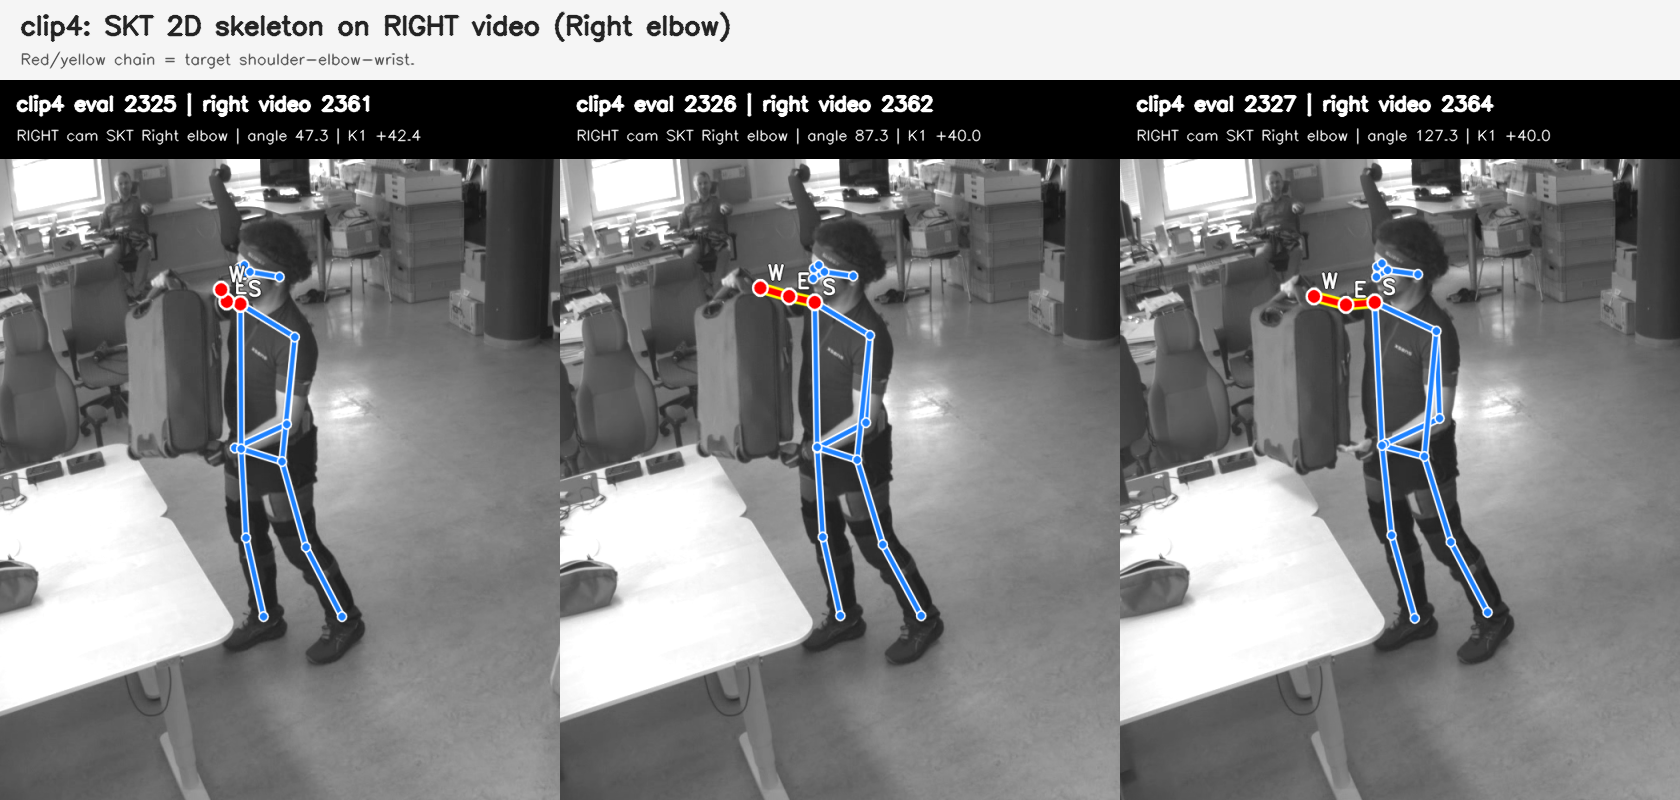
\includegraphics[width=\linewidth]{thesis_skt_high_delta_right_elbow_frames.png}
    \caption{Right-elbow high-delta interval.}
  \end{subfigure}
  \caption{Representative SKT high-delta diagnostic frames projected onto the original video view. These examples indicate that some large motion deltas are caused by local keypoint instability around the elbow chain rather than by physically implausible whole-body motion.}
  \label{fig:skt_high_delta_cases}
\end{figure}

\subsection{Limitations}

Four limitations of the present study set the boundary inside which all
quantitative results above should be read; they are stated explicitly here
so that the conclusion in Section~\ref{sec:conclusion} can rest on
honestly scoped evidence rather than on an over-generalised claim.
\emph{First}, all results come from a single subject performing a single
controlled recording in a manufacturing-like environment; the
between-method ranking should therefore be read as supported on this
dataset rather than as a general statement about every operator,
clothing style, lighting condition, or camera distance.
\emph{Second}, the deepest motion-space analysis focuses on the elbow,
which is the joint that the project investigated most carefully and the
joint whose Xsens calibration limitation is best quantified; the
motion-space numbers for the shoulder, hip, and knee are reported but
should be read with weaker confidence than the elbow numbers because
their reference floor is less well characterised.
\emph{Third}, the evaluation outputs depend on the smoothing window, the
segment-detection thresholds, and the constant-offset assumption used for
time alignment; the pipeline records these settings explicitly in the run
configuration so that any future work can rerun the same comparison under
different choices, and the synchronisation analysis in
Section~\ref{sec:data_setup} shows that the constant-offset assumption is
adequate for this recording but does not prove it for longer recordings.
\emph{Fourth}, Xsens is used throughout as an external comparison
reference and not as physical ground truth; the absolute angle errors are
therefore interpreted alongside the Xsens self-consistency floor
established in Section~\ref{sec:data_setup} rather than as direct error
against a true biomechanical zero.

\subsection{Implications for Real-time Deployment}

The deployment path that follows most cleanly from the above is to
prioritise getting the calibrated SKT pipeline running efficiently on
GPU hardware before treating learning-based pose models as
replacements rather than as optional stabilisers.
The concrete engineering steps are well-established: export the 2D pose
model to TensorRT, move video decoding and preprocessing onto the GPU,
and keep triangulation and joint-angle computation lightweight enough to
remain in the streaming budget; lightweight real-time pose models such
as RTMPose \cite{jiang2023rtmpose} make this direction realistic at the
2D-detection stage, although the final reportable number must be
end-to-end latency rather than model inference time alone, because
decoding, preprocessing, and post-processing each consume a measurable
share of the per-frame budget.
Once this baseline streams reliably, the two natural extensions are
(i) integrating a learning-based pose head -- of the FastSAM3D family --
as an optional smoothing or fallback signal when SKT quality flags drop
below an acceptable threshold, and (ii) introducing transformer-based
temporal priors to repair the keypoint-chain failures identified in the
high-delta analysis above; both extensions are framed here as
\emph{stabilisers on top of} the calibrated stereo baseline rather than
as replacements for it, because the deployment-geometry advantages
discussed in Section~7.2 do not transfer to a pure monocular pipeline
without additional scale/coordinate work.

\clearpage
% =============================================================
\section{Conclusion and Future Work}
\label{sec:conclusion}
% =============================================================

\subsection{Conclusion}

This thesis evaluates 3D human pose estimation for manufacturing-oriented
ergonomic monitoring using a three-axis framework -- angle-space,
motion-space, and position-space -- against an Xsens reference whose
calibration limitation is explicitly quantified rather than ignored.
On the single-subject manufacturing recording used here, the
learning-based monocular FastSAM3D pipeline delivers better
agreement-track numbers (mean angle MAE 15.4\degr\ vs.\ 17.6\degr; mean
K=6 motion Pearson 0.64 vs.\ 0.38; segment ROM error 14.9\degr\ vs.\
26.9\degr) than the calibrated stereo SKT pipeline.
SKT nevertheless retains the only metric-scale 3D output among the
evaluated pipelines and is the only pipeline that exposes per-frame
geometric quality signals usable for downstream quality gating, so it
remains the right choice when deployment requires real units or
self-reported reliability rather than only joint-angle smoothness.
The substantive conclusion is therefore not a single recommended method
but a deliberate split: learning-based monocular pose is competitive
when the deployment task is restricted to joint angles and short-term
motion, while calibrated stereo is necessary when the deployment task
extends to metric 3D scale and explainable per-frame quality, and a
future ergonomic monitoring system is likely to want both -- learned
priors for body-pose stability, stereo geometry for scale and
deployment transparency.

\subsection{Future Work}

Three follow-up directions are required before the present results can
be claimed as generally applicable rather than as evidence for a single
controlled recording.

\begin{enumerate}[leftmargin=1.2cm]
  \item \textbf{Validation on additional recordings and subjects.}
        Repeat the same three-axis protocol on at least one additional
        operator, additional clothing, additional lighting, and an
        unscripted task, in order to test whether the FastSAM3D
        agreement-track advantage generalises and whether the SKT
        high-delta failure modes recur in the same shoulder--elbow--wrist
        chain across subjects.
  \item \textbf{Real-time GPU deployment of SKT with optional learned
        stabilisers.} Move the SKT 2D backbone to TensorRT and the
        decoding/preprocessing onto the GPU, measure end-to-end streaming
        latency rather than model inference time alone, and then evaluate
        a FastSAM3D-style learned head as an optional smoothing or
        fallback signal triggered when SKT quality flags drop below the
        deployment threshold.
  \item \textbf{Beyond-elbow motion analysis and connection to a complete
        ergonomic risk score.} Extend the motion-space analysis to the
        shoulder, hip, and knee with the same reference-floor
        quantification that this thesis applies to the elbow, and then
        connect the resulting joint-angle stream to a full ergonomic
        risk score (e.g.\ RULA, REBA) rather than to RULA-bin agreement
        alone, so that pose-estimation quality and downstream
        risk-classification quality can be reported as a single
        deployment-relevant pipeline.
\end{enumerate}

\subsection{Recommended Next-stage Experimental Protocol}

To make the validation-on-new-datasets step above repeatable rather than
ad hoc, this subsection consolidates the working protocol used in the
present recording into a five-stage checklist
(Table~\ref{tab:validation_checklist}) that future datasets should run
\emph{in order}, with each stage gating the next.
The protocol enforces two methodological principles that emerged from
the present study.
The first principle is that data-ingestion integrity (orientation,
frame-ID re-pairing, timestamp monotonicity, calibration compatibility)
must be verified before any accuracy number is computed, because the
most expensive class of failure in the present pipeline is
mis-interpreting an ingestion bug as a pose-estimation result.
The second principle is that algorithmic changes and protocol changes
must be evaluated separately: if SKT is later modified with stronger
2D-keypoint filtering or a temporal repair module, the same K-frame
motion-delta protocol must be rerun before and after the modification
so that the comparison is fair, and if a new learning-based method is
added, its coordinate convention and filtering state must be recorded
before it is included in the position-space analysis.

\begin{table}[!htbp]
  \centering
  \caption{Five-stage validation checklist for extending the present thesis evaluation to new manufacturing recordings. Stages should be executed in order; each stage gates the next.}
  \label{tab:validation_checklist}
  \small
  \begin{tabularx}{\linewidth}{p{3.2cm}XX}
    \toprule
    Stage & What should be checked & Why it matters \\
    \midrule
    Dataset validation
    & Video orientation, hardware frame IDs, metadata timestamps, synchronised frame count, and camera calibration compatibility.
    & Prevents data-ingestion errors from being mis-interpreted as pose-estimation errors. \\
    Time alignment
    & Automatic offset curves on three independent scores, residual lag at the beginning and end of the recording, and common valid intervals.
    & Ensures that motion-space metrics compare the same physical movement period. \\
    Method comparison
    & Angle MAE, K-frame motion agreement at $K\in\{1,6,12,25\}$, segment ROM and DTW, and position-space diagnostics for every method.
    & Keeps the comparison multi-dimensional and avoids over-ranking methods by a single metric. \\
    Failure analysis
    & High-delta frames, occlusion cases, camera distance, and left--right keypoint consistency.
    & Connects quantitative outliers to concrete visual causes and guides targeted SKT repair work. \\
    Deployment check
    & End-to-end streaming latency, GPU preprocessing, model inference time, and stability under streaming input.
    & Tests whether the method can move from offline evaluation toward real-time ergonomic monitoring. \\
    \bottomrule
  \end{tabularx}
\end{table}

The final thesis version should therefore deliver two distinct kinds of
evidence rather than a single aggregate error number.
The first is \emph{quantitative agreement} across several recordings and
movement types, run through the checklist above so that the comparison
remains multi-dimensional and protocol-controlled.
The second is \emph{diagnostic evidence} that exposes when and why each
pipeline fails and which subsystem is responsible, of the kind that
Section~\ref{sec:discussion} presented for the SKT high-delta cases.
This combination is the right level of evidence for ergonomic deployment
in manufacturing, because a practical monitoring system needs not only
to be accurate on average but also to know -- and to expose -- when its
output should not be trusted.

\clearpage
% =============================================================
\appendix
\clearpage
% =============================================================

\section{Stereo Calibration Parameters}
\label{app:calibration}

The numerical calibration values reported below are the optimised parameters
that all SKT experiments in the thesis use as fixed input; the
binary form is stored at \texttt{shared/camera\_params.npz} and is loaded
directly by the pose pipeline.
The intrinsic matrices follow the OpenCV convention $K = [[f_x, 0, c_x];
[0, f_y, c_y]; [0,0,1]]$ in pixels, the distortion vectors follow the
14-parameter rational model used by OpenCV's \texttt{cv2.calibrateCamera}
(only the first 8 entries are non-zero in this calibration), and the
stereo extrinsics give the rotation $R$ and translation $T$ that map a
3D point from the left to the right camera frame in centimetres.

\begin{table}[!htbp]
  \centering
  \caption{Left and right camera intrinsic matrices (pixels) and the stereo extrinsic baseline.}
  \label{tab:calib_intrinsics}
  \small
  \begin{tabular}{lcc}
    \toprule
    Quantity & Left camera & Right camera \\
    \midrule
    $f_x$ (pixels)            & 1130.27 & 1129.01 \\
    $f_y$ (pixels)            & 1130.35 & 1129.63 \\
    $c_x$ (pixels)            & 1019.32 & 1028.31 \\
    $c_y$ (pixels)            &  825.72 &  826.35 \\
    \midrule
    Stereo baseline $\|T\|$   & \multicolumn{2}{c}{41.27\,cm} \\
    Image resolution          & \multicolumn{2}{c}{2048 $\times$ 1536} \\
    Distortion model          & \multicolumn{2}{c}{OpenCV rational (14-parameter)} \\
    \bottomrule
  \end{tabular}
\end{table}

The stereo rotation $R$ deviates from the identity by less than 0.011
radians on each off-diagonal entry, consistent with a near-aligned
parallel-baseline rig, and the translation vector
$T \approx [-41.27, -0.03, 0.04]^T$\,cm confirms that the baseline is
dominated by the $x$ axis as designed.
The essential matrix $E$ and fundamental matrix $F$ recorded in
\texttt{camera\_params.npz} are derived from $R$ and $T$ together with
the two intrinsic matrices and are not duplicated here.
The full distortion coefficients and the original calibration session
metadata (target type, number of valid views, per-view reprojection
residuals) are stored alongside the matrices in the same NPZ file.

\FloatBarrier
\clearpage
\section{Sensitivity Analyses}
\label{app:sensitivity}

The headline numbers reported in Section~\ref{sec:results} depend on
three parameter choices made in the evaluation pipeline: the camera-side
smoothing window, the activity-segment detection threshold, and the
DTW preprocessing convention.
This appendix reports how the SKT motion and segment-level numbers move
when each choice is varied, so that the reader can judge how brittle the
conclusion is.

\begin{table}[!htbp]
  \centering
  \caption{Sensitivity of SKT motion-space and segment-level numbers to the camera-side moving-average smoothing window, on the present recording. The 200\,ms and 300\,ms rows are identical because both round to a 3-frame centred window at 12.5\,fps.}
  \label{tab:sens_smoothing}
  \footnotesize
  \setlength{\tabcolsep}{4pt}
  \resizebox{\linewidth}{!}{%
  \begin{tabular}{lcccc}
    \toprule
    Window & Frames & SKT K=6 Pearson (L/R) & SKT ROM MAE (L/R, \degr) & K=1 quiet std (L/R, \degr) \\
    \midrule
    100\,ms & 1 & -- / --   & 38.4 / 33.3 & --   / --   \\
    200\,ms & 3 & 0.41 / 0.40 & 19.3 / 21.3 & 7.0 / 6.6 \\
    300\,ms & 3 & 0.41 / 0.40 & 19.3 / 21.3 & 7.0 / 6.6 \\
    400\,ms & 5 & 0.43 / 0.42 & 16.4 / 21.8 & 4.4 / 4.5 \\
    \bottomrule
  \end{tabular}%
  }
\end{table}

The 200\,ms working point chosen in the main body is the
literature-supported rule of thumb for non-explosive human motion; a
400\,ms window further reduces SKT quiet-frame jitter below the
$<$5\degr/frame validation target at the cost of a slightly weaker
short-term motion signal, and is reported here as the
``conservative-smoothing'' alternative for future runs.

\begin{table}[!htbp]
  \centering
  \caption{Sensitivity of detected segment counts to the activity-detection threshold (applied to the Xsens-derived reference K-frame deltas).}
  \label{tab:sens_segments}
  \small
  \begin{tabular}{lcc}
    \toprule
    Activity threshold (\degr) & Left-elbow segments & Right-elbow segments \\
    \midrule
    8  & 5  & 7  \\
    10 (default) & 8 & 9 \\
    12 & 13 & 15 \\
    \bottomrule
  \end{tabular}
\end{table}

Segment counts vary by a factor of roughly 2--3 across the tested
threshold range, but the cross-method ranking inside each row is stable:
FastSAM3D maintains the lowest segment ROM MAE and DTW distance
regardless of the threshold setting, so the main-body conclusion does
not depend on the specific threshold value chosen.
The DTW preprocessing sweep (\texttt{mean\_l2}, \texttt{mean}, and
\texttt{none}) confirms that the mean-subtracted, L2-normalised
convention adopted in the main body is the version under which the
XsensNative-vs-XsensFair anchor DTW remains near zero; without L2
normalisation the DTW distance becomes dominated by amplitude rather
than by shape, which is the explicit motivation for the chosen
preprocessing.

\FloatBarrier
\clearpage
\section{Implementation and Reproducibility Notes}
\label{app:repro}

The standalone evaluation workflow is implemented in
\texttt{00\_pose\_pipeline/}.
For the present dataset, the main reproduction command is:
\begin{footnotesize}
\begin{verbatim}
/opt/anaconda3/envs/pose/bin/python \
  00_pose_pipeline/src/run_pipeline.py \
  --config \
  00_pose_pipeline/configs/current_2025_ergonomics.yaml \
  --stages \
  validate,offset,angle,motion,segment,scatter
\end{verbatim}
\end{footnotesize}

The configuration file records the dataset-specific choices that
otherwise must be inferred from prose alone: the 180\degr\ video
rotation, the hardware-frame-ID synchronisation rule, the metadata
timestamp-parsing convention, the calibration NPZ path, the per-system
smoothing settings, the K-frame list $\{1,6,12,25\}$, the
activity-detection threshold, and the automatic offset-search range.
Generated outputs are stored under \texttt{00\_pose\_pipeline/runs/}
and include both the headline tables/figures referenced from the main
body and the per-stage diagnostics that drive Section~\ref{sec:discussion}.

Figure~\ref{fig:residual_lag_check} reports a residual lag diagnostic
that the pipeline can produce after the selected constant offset has
been applied; it is not a headline result but it documents the
sanity-check evidence used to defend the constant-offset assumption in
Section~\ref{sec:data_setup}.

\begin{figure}[!htbp]
  \centering
  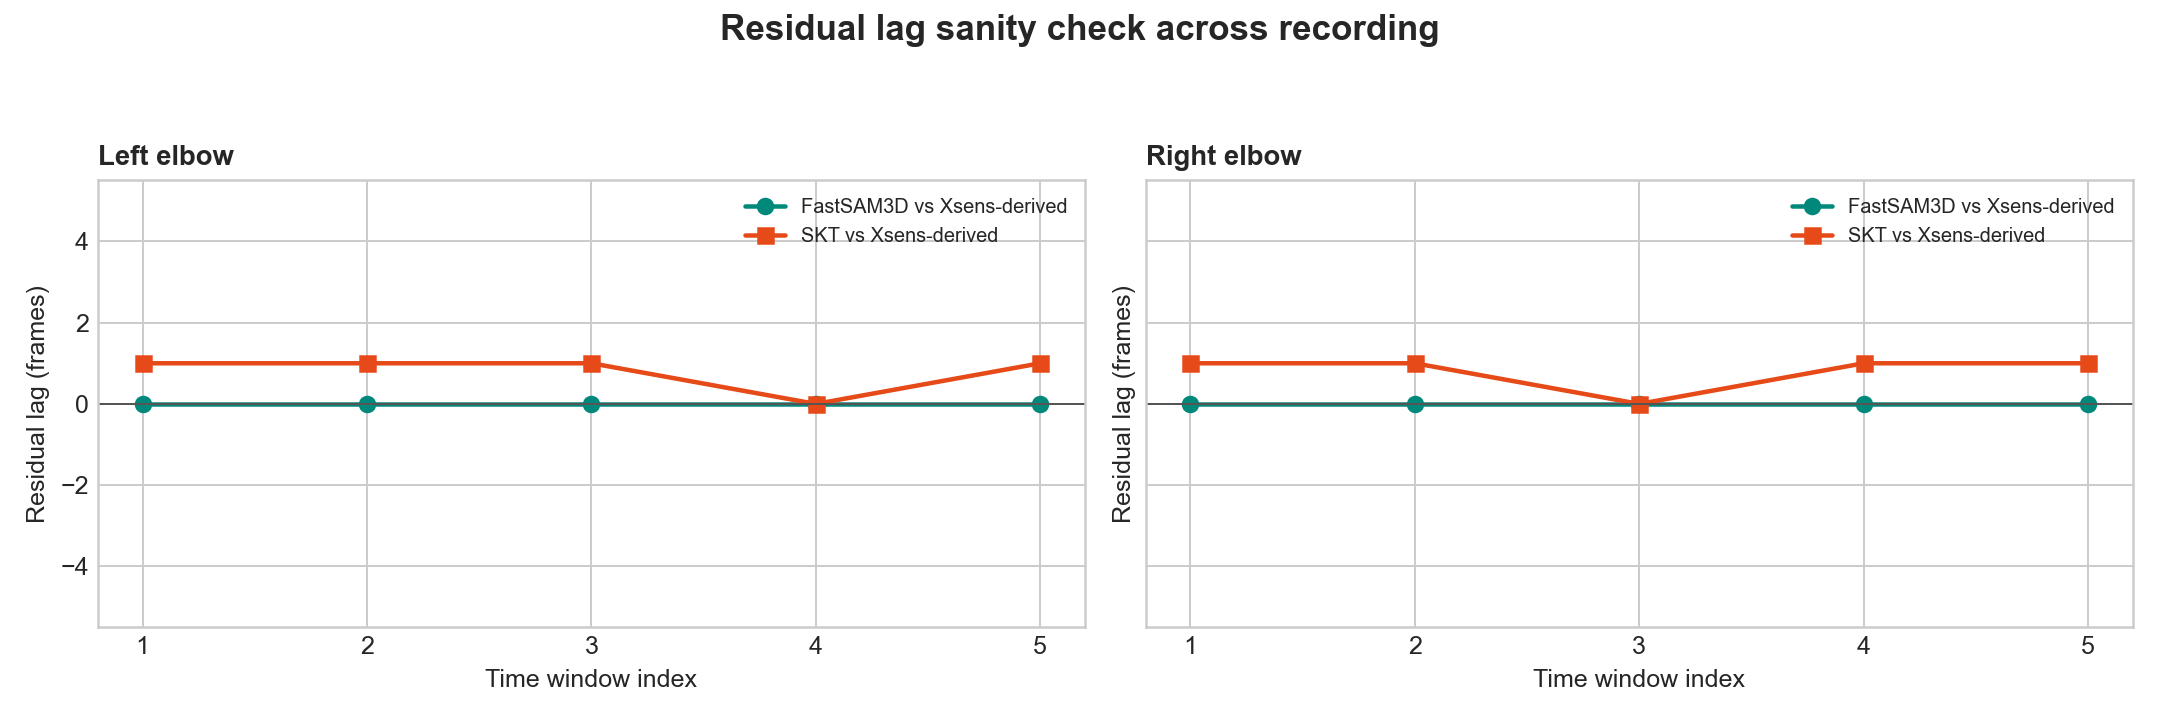
\includegraphics[width=\linewidth]{thesis_residual_lag_drift_check.png}
  \caption{Residual lag sanity check after applying the selected constant offset. The figure supports the assumption that a constant offset is adequate for the present recording, while explicitly acknowledging that future longer or multi-take recordings should rerun this check.}
  \label{fig:residual_lag_check}
\end{figure}

\FloatBarrier
\clearpage
\section{Claim-evidence Self-review}
\label{app:claim_evidence}

The table below maps every major thesis claim back to its supporting
evidence in this draft, following the
``Claim $|$ Evidence $|$ Status'' convention recommended for
adversarial paper review.
Claims marked \emph{Needs evidence} are stated as open items rather
than as supported conclusions, and the conclusion in
Section~\ref{sec:conclusion} is restricted to the claims marked
\emph{Supported}.

\begin{table}[H]
  \centering
  \caption{Claim-evidence map for the present thesis draft.}
  \label{tab:claim_evidence}
  \small
  \renewcommand{\arraystretch}{1.12}
  \begin{tabularx}{\linewidth}{p{4.0cm}Xp{1.9cm}}
    \toprule
    Claim & Evidence used in this draft & Status \\
    \midrule
    FastSAM3D is stronger than SKT in angle-space on the present dataset.
    & Table~\ref{tab:angle_summary} and Figure~\ref{fig:angle_summary_plot}: 15.4\degr\ mean MAE vs.\ 17.6\degr.
    & Supported \\
    FastSAM3D is stronger than SKT in K=6 motion-space agreement.
    & Table~\ref{tab:motion_summary}, Figure~\ref{fig:motion_k6_summary_plot}, and Figure~\ref{fig:k6_elbow_scatter}: mean Pearson 0.644 vs.\ 0.379; elbow correlations 0.54/0.69 vs.\ 0.39/0.39.
    & Supported \\
    SKT retains a position-space and interpretability advantage.
    & Table~\ref{tab:position_summary}, Figure~\ref{fig:position_diagnostic_plot}, and the SKT method design; SKT uses calibrated stereo scale and exposes per-frame geometric quality signals.
    & Supported \\
    A constant cross-system offset is adequate for the current recording.
    & Figure~\ref{fig:offset_search}, Figure~\ref{fig:first_last_delta}, and Figure~\ref{fig:residual_lag_check}; the three independent offset scores converge within $\sim$0.04\,s.
    & Supported for present recording \\
    SKT high-delta points are caused by local keypoint-chain instability.
    & Figure~\ref{fig:skt_high_delta_cases}: diagnostic frames show partial wrist occlusion, large camera distance, and inconsistent left/right elbow-chain detection during the high-delta intervals.
    & Supported qualitatively \\
    The SKT vs FastSAM3D ranking is robust to smoothing and segmentation parameters.
    & Appendix~\ref{app:sensitivity}: sensitivity tables across smoothing windows and activity thresholds preserve the FastSAM3D $>$ SKT ranking.
    & Supported \\
    Results generalise to manufacturing environments broadly.
    & Only one controlled single-subject dataset is evaluated.
    & Needs evidence \\
    Full RULA automation is solved.
    & Only continuous angle MAE and RULA-like bin agreement are reported; RULA scoring requires additional load/twist/repetition information.
    & Not claimed \\
    \bottomrule
  \end{tabularx}
\end{table}

\clearpage

\begin{thebibliography}{99}

\bibitem{mcatamney1993rula}
L.~McAtamney and E.~N.~Corlett,
\textit{RULA: a survey method for the investigation of work-related upper limb disorders},
Applied Ergonomics, vol.~24, no.~2, pp.~91--99, 1993.

\bibitem{menolotto2020motion}
M.~Menolotto, D.-S.~Komaris, S.~Tedesco, B.~O'Flynn, and M.~Walsh,
\textit{Motion capture technology in industrial applications: A systematic review},
Sensors, vol.~20, no.~19, article 5687, 2020.

\bibitem{yu2019joint}
Y.~Yu, X.~Yang, H.~Li, X.~Luo, and H.~Guo,
\textit{Joint-level vision-based ergonomic assessment tool for construction workers},
Journal of Construction Engineering and Management, vol.~145, no.~5, 2019.

\bibitem{menanno2024ergonomic}
M.~Menanno, C.~Riccio, V.~Benedetto, and G.~Palmieri,
\textit{An ergonomic risk assessment system based on 3D human pose estimation and collaborative robot},
Applied Sciences, vol.~14, no.~11, article 4823, 2024.

\bibitem{quesada2026supporting}
A.~Quesada Diaz, A.~Iriondo Pascual, L.~Hanson, D.~H{\"o}gberg, and A.~Syberfeldt,
\textit{Supporting ergonomics evaluations in manufacturing: A comparison of computer vision- and IMU-based motion capture},
IOP Conference Series: Materials Science and Engineering, vol.~1342, article 012053, 2026.

\bibitem{iriondo2024development}
A.~Iriondo Pascual, L.~Hanson, D.~H{\"o}gberg, E.~Brolin, and A.~Syberfeldt,
\textit{Development and initial usability evaluation of a digital tool for simulation-based multi-objective optimization of productivity and worker well-being},
Advanced Engineering Informatics, vol.~60, article 102726, 2024.

\bibitem{iriondo2025integrating}
A.~Iriondo Pascual, L.~Hanson, E.~Brolin, D.~H{\"o}gberg, and A.~Syberfeldt,
\textit{Integrating motion capture and digital human modelling tools for worker ergonomics assessment: A case study from experimental lab to real-world manufacturing},
Lecture Notes in Computer Science, vol.~15828, pp.~324--333, 2025.

\bibitem{filippeschi2017survey}
A.~Filippeschi, N.~Schmitz, M.~Miezal, G.~Bleser, E.~Ruffaldi, and D.~Stricker,
\textit{Survey of motion tracking methods based on inertial sensors: A focus on upper limb human motion},
Sensors, vol.~17, no.~6, article 1257, 2017.

\bibitem{roetenberg2009xsens}
D.~Roetenberg, H.~Luinge, and P.~Slycke,
\textit{Xsens MVN: Full 6DOF human motion tracking using miniature inertial sensors},
Xsens Technologies technical report, 2009.

\bibitem{cao2019openpose}
Z.~Cao, G.~Hidalgo, T.~Simon, S.-E.~Wei, and Y.~Sheikh,
\textit{OpenPose: Realtime multi-person 2D pose estimation using part affinity fields},
IEEE Transactions on Pattern Analysis and Machine Intelligence,
vol.~43, no.~1, pp.~172--186, 2019.

\bibitem{jiang2023rtmpose}
T.~Jiang, P.~Lu, L.~Zhang, N.~Ma, R.~Han, C.~Lyu, Y.~Li, and K.~Chen,
\textit{RTMPose: Real-time multi-person pose estimation based on MMPose},
arXiv preprint arXiv:2303.07399, 2023.

\bibitem{pavllo20193d}
D.~Pavllo, C.~Feichtenhofer, D.~Grangier, and M.~Auli,
\textit{3D human pose estimation in video with temporal convolutions and semi-supervised training},
Proceedings of the IEEE/CVF Conference on Computer Vision and Pattern Recognition, pp.~7753--7762, 2019.

\bibitem{zhu2023motionbert}
W.~Zhu, X.~Ma, Z.~Liu, L.~Liu, W.~Wu, and Y.~Wang,
\textit{MotionBERT: A unified perspective on learning human motion representation},
Proceedings of the IEEE/CVF International Conference on Computer Vision, pp.~15085--15099, 2023.

\bibitem{yang2026fastsam3d}
T.~Yang, S.~He, H.~Jing, J.~Yang, Z.~Liu, C.~Zou, and Y.~Wang,
\textit{Fast SAM 3D Body: Accelerating SAM 3D Body for Real-Time Full-Body Human Mesh Recovery},
arXiv preprint arXiv:2603.15603, 2026.

\bibitem{hartley2004multiple}
R.~Hartley and A.~Zisserman,
\textit{Multiple View Geometry in Computer Vision},
2nd ed., Cambridge University Press, 2004.

\bibitem{hirschmuller2007sgbm}
H.~Hirschm{\"u}ller,
\textit{Stereo processing by semiglobal matching and mutual information},
IEEE Transactions on Pattern Analysis and Machine Intelligence,
vol.~30, no.~2, pp.~328--341, 2007.

\bibitem{kabsch1976solution}
W.~Kabsch,
\textit{A solution for the best rotation to relate two sets of vectors},
Acta Crystallographica, Section A, vol.~32, pp.~922--923, 1976.

\bibitem{sakoe1978dtw}
H.~Sakoe and S.~Chiba,
\textit{Dynamic programming algorithm optimization for spoken word recognition},
IEEE Transactions on Acoustics, Speech, and Signal Processing,
vol.~26, no.~1, pp.~43--49, 1978.

\bibitem{perezluque2026reaching}
E.~P{\'e}rez Luque, S.~Lee, D.~H{\"o}gberg, J.~Yang, and M.~Lamb,
\textit{Predicting human upper extremity reaching motions: Comparison of optimization-based method and heuristic method},
International Journal of Human--Computer Interaction, 2026.
DOI: 10.1080/10447318.2026.2632154.

\end{thebibliography}

\end{document}

% =============================================================

\documentclass[12pt,a4paper]{article}

\usepackage[margin=2.5cm]{geometry}
\usepackage{fontspec}
\defaultfontfeatures{Ligatures=TeX}
\usepackage{amsmath,amssymb}
\usepackage{siunitx}
\usepackage{booktabs}
\usepackage{graphicx}
\usepackage{subcaption}
\usepackage[table]{xcolor}
\usepackage{hyperref}
\usepackage{microtype}
\usepackage{parskip}
\usepackage{enumitem}
\usepackage{array}
\usepackage{float}
\usepackage{tabularx}
\usepackage{setspace}
\usepackage{placeins}
\usepackage{caption}

\hypersetup{colorlinks=true, linkcolor=blue!70!black, urlcolor=blue!70!black, citecolor=green!50!black}
\graphicspath{{figures/}}
\emergencystretch=2em
\setstretch{1.06}
\setlength{\textfloatsep}{1.1em plus 0.25em minus 0.2em}
\setlength{\floatsep}{1.0em plus 0.25em minus 0.2em}
\setlength{\intextsep}{1.0em plus 0.25em minus 0.2em}
\captionsetup{font=small, labelfont=bf}

\definecolor{goodcolor}{rgb}{0.00,0.38,0.18}
\definecolor{warncolor}{rgb}{0.55,0.27,0.07}
\definecolor{badcolor}{rgb}{0.65,0.10,0.10}
\newcommand{\good}[1]{\textcolor{goodcolor}{\textbf{#1}}}
\newcommand{\warn}[1]{\textcolor{warncolor}{\textbf{#1}}}
\newcommand{\bad}[1]{\textcolor{badcolor}{\textbf{#1}}}
\newcommand{\degr}{\ensuremath{^\circ}}

\title{\textbf{Posture and Activity Detection in Manufacturing Environments\\Using 3D Vision and AI}}
\author{Fanbo Meng\\
\small Chalmers University of Technology\\
\small In collaboration with Viscando AB}
\date{Master's Thesis Draft, June 2026}

\begin{document}
\maketitle
\tableofcontents
\newpage

% =============================================================
\section*{Abstract}
% =============================================================

Ergonomic risk assessment in manufacturing demands pose-estimation systems
that are spatially accurate, temporally consistent, and interpretable at the
joint-angle level, yet the dominant evaluation practice in the pose-estimation
literature still relies on a single distance metric such as Mean Per-Joint
Position Error, which is not sufficient to decide whether a method is fit for
ergonomic monitoring.
This thesis revisits 3D human pose estimation for manufacturing settings by
comparing a calibrated stereo keypoint triangulation pipeline (SKT) with a
monocular learning-based pipeline (FastSAM3D); an Xsens inertial motion-capture
suit is used as an external reference system rather than as absolute ground
truth, because its body-model calibration introduces systematic angle offsets
that must be acknowledged in the evaluation design.
The evaluation is organized around three complementary axes -- angle-space
accuracy, motion-space consistency, and position-space geometry -- and the
motion-space axis is built on K-frame angle deltas
($\Delta_K\theta_t = \theta_t-\theta_{t-K}$), which cancel the static Xsens
offset by differencing and expose true short-term motion agreement.
On a single-subject manufacturing recording of 2801 synchronized stereo frame
pairs over 248.8\,s, FastSAM3D achieves lower mean angle MAE than SKT across
eight body angles (15.4\degr\ vs.\ 17.6\degr) and stronger K=6 motion-delta
correlation with the Xsens-derived reference (mean Pearson 0.64 vs.\ 0.38;
right-elbow Pearson 0.69 vs.\ 0.39).
This angle and motion advantage is attributed to FastSAM3D's learned
body-shape and motion-continuity priors, which absorb anatomical constraints
from large training corpora and consequently suppress the per-frame keypoint
jitter that a frame-independent geometric triangulation pipeline propagates
directly into its angle estimates.
SKT, by contrast, retains a clear position-space advantage: its 3D coordinates
inherit metric scale directly from the calibrated stereo baseline without any
external alignment step, and the per-frame geometric quality signals it
exposes~-- epipolar error, reprojection error, triangulation confidence~--
provide deployment-ready reliability indicators that a monocular learning-based
pipeline does not offer natively.
These findings indicate that the two approaches are complementary rather than
interchangeable: learned monocular pose estimation is the more competitive
choice when angle accuracy and temporal motion smoothness are the primary
requirements, while calibrated stereo triangulation remains essential when
metric 3D coordinates and transparent per-frame reliability are needed for
downstream ergonomic quality control.

% =============================================================
\newpage
\section{Introduction}
% =============================================================

\subsection{Motivation}

Work-related musculoskeletal disorders remain one of the dominant
occupational-health burdens in manufacturing, and the established
countermeasure is repeated ergonomic risk assessment of operators while they
perform actual production tasks.
The standard observational instruments for such assessment, including the
Rapid Upper Limb Assessment (RULA), depend on a trained observer who manually
classifies joint postures into discrete risk categories
\cite{mcatamney1993rula}; this practice is labour-intensive, observer
dependent, and impossible to deploy at the temporal resolution that modern
just-in-time production demands.
Camera-based 3D human pose estimation offers a path toward continuous,
non-intrusive ergonomic monitoring, because the joint angles needed for RULA
and similar instruments can in principle be read directly from a body
skeleton reconstructed from video.

Realising this promise on the factory floor changes what counts as ``good''
pose estimation.
The dominant benchmarks in the pose-estimation literature reward
visually-plausible skeletons and low Mean Per-Joint Position Error (MPJPE) on
short, well-lit, frontal-view clips; an ergonomic monitoring system, however,
must produce joint-angle estimates that are temporally stable across long
shifts, robust to occlusion and dark workwear, and traceable to interpretable
quality signals when downstream automated risk scoring is involved.
This thesis therefore treats pose estimation as a measurement problem that
sits between multi-view geometry, learning-based vision, and application-level
ergonomic evaluation, and it organises its evaluation around the properties
that ergonomic deployment actually requires rather than around a single
geometric distance metric.

\subsection{Problem Statement and Scope}

The thesis investigates 3D body-keypoint and joint-angle estimation from a
calibrated stereo camera setup in a manufacturing-like environment, with the
deployment target being downstream ergonomic risk monitoring rather than
generic motion reconstruction.
The primary pose-estimation method developed in the thesis is Sparse
Keypoint Triangulation (SKT), in which a 2D pose detector is run on
synchronised left and right video streams and the matched keypoints are
triangulated into 3D under the calibrated stereo geometry; the study then
benchmarks SKT against a monocular learning-based pipeline (FastSAM3D).

A central methodological constraint is that no laboratory-grade optical
motion-capture system was available for the full manufacturing recording, so
this thesis adopts an Xsens inertial suit as an \emph{external reference
system}, deliberately avoiding the language of ``absolute ground truth''.
This wording is not cosmetic: the Xsens body model is calibrated through a
short on-subject procedure that can absorb true global orientation and
introduce a systematic per-joint offset, most visibly at the elbow.
Reporting only absolute joint-angle MAE against such a reference therefore
risks transferring the reference's calibration bias into a verdict about the
vision pipeline, and the evaluation design must counter this by reporting
relative-change metrics (frame-to-frame K-frame angle deltas) in parallel
with absolute angles, since differencing cancels any static offset that the
two systems may carry.

\subsection{Research Questions}

The thesis is structured around three research questions:

\begin{enumerate}[label=\textbf{RQ\arabic*:}, leftmargin=1.8cm]
  \item How accurately can a calibrated stereo keypoint triangulation
        pipeline (SKT) recover the eight ergonomically relevant upper- and
        lower-body joint angles in a manufacturing-style recording, when
        absolute and motion-space accuracy are reported in parallel against
        an Xsens-derived reference?
  \item Under a unified evaluation protocol (shared timeline, common
        smoothing policy, identical reference), how does the geometry-based
        SKT pipeline compare with the learning-based FastSAM3D pipeline in
        (i) absolute angle accuracy and (ii) K-frame motion consistency at
        $K\in\{1,6,12,25\}$ frames?
  \item Which pipeline properties beyond raw accuracy -- in particular
        per-frame quality signals, metric scale, and resilience to
        occlusion and low-texture industrial backgrounds -- decide whether
        a method is fit for real-time ergonomic monitoring on GPU hardware?
\end{enumerate}

\subsection{Contributions}

In addressing the three research questions, the thesis makes the following
contributions:

\begin{itemize}[leftmargin=1.2cm]
  \item \textbf{A reproducible stereo pose pipeline (SKT)} that combines
        synchronised 2D keypoint detection, calibrated DLT triangulation,
        three-point geometric joint-angle computation, and per-frame
        geometry-aware quality signals (triangulation confidence, epipolar
        error, reprojection error) that can drive downstream quality gating.
  \item \textbf{A three-axis evaluation framework} -- angle-space, motion-space,
        position-space -- that exposes method-property tradeoffs which a single
        MPJPE-style metric would conceal, and that is reusable across other
        vision pipelines on the same dataset.
  \item \textbf{An explicit cross-system synchronisation and filtering protocol},
        including automatic temporal-offset estimation against three independent
        scores, hardware-frame-ID re-pairing for non-monotonic stereo
        timestamps, and a per-system smoothing policy (no extra smoothing on
        the already heavily filtered Xsens reference, unified 200\,ms moving
        average on the camera-based methods).
  \item \textbf{An empirical comparison} that finds the monocular learning-based
        FastSAM3D pipeline more competitive than the calibrated stereo SKT on
        both angle MAE and K-frame motion correlation for this manufacturing
        recording, while showing that SKT retains an irreplaceable advantage
        in metric 3D scale and in geometry-aware quality control needed for
        deployment.
\end{itemize}

\subsection{Thesis Structure}

The remainder of the thesis is organised as follows.
Section~\ref{sec:background} reviews relevant work on 3D human pose
estimation, vision-based ergonomic assessment, and reference-system
limitations.
Section~\ref{sec:data_setup} describes the stereo capture system, the
2025 ergonomics dataset, the Xsens reference data, and the cross-system
time-synchronisation procedure.
Section~\ref{sec:methods} presents the two evaluated pose-estimation
pipelines (SKT and FastSAM3D).
Section~\ref{sec:evaluation} defines the three-axis evaluation framework and
the unified filtering policy.
Section~\ref{sec:results} reports the angle-space, motion-space,
segment-level, and position-space results, and synthesises them across
methods.
Section~\ref{sec:discussion} discusses applicability boundaries, failure
modes, and limitations, and
Section~\ref{sec:conclusion} concludes and outlines future work.

\clearpage
% =============================================================
\section{Background and Related Work}
\label{sec:background}
% =============================================================

\subsection{3D Human Pose Estimation}

3D human pose estimation recovers either explicit body keypoints or
parametric body-model parameters from one or several camera streams, and the
existing literature divides clearly along whether the recovery uses one view
or multiple views.
Monocular approaches estimate 3D pose from a single image or video, either
through a two-stage 2D--detection + 3D--lifting pipeline or through an
end-to-end regression that maps image features directly to 3D coordinates.
Real-time 2D pose estimators such as OpenPose and RTMPose have established
that the 2D detection stage can be made fast and accurate enough for online
use \cite{cao2019openpose,jiang2023rtmpose}, and temporal 3D models such as
VideoPose3D and MotionBERT have shown that body-motion priors can be learned
from large pose-sequence corpora and used to stabilise the lifting step
\cite{pavllo20193d,zhu2023motionbert}.
The structural limitation of any monocular pipeline, however, is that the
absolute distance from camera to subject is not directly observed; depth and
metric scale must be inferred from learned body proportions or recovered
through an external alignment step, which is acceptable for visual
animation but problematic for ergonomic measurement.

Stereo and multi-view approaches replace this scale ambiguity with explicit
multi-view geometry.
In a calibrated two-camera setup, an epipolar relation constrains where a
point seen in the left view must appear in the right view, and the intersection
of the two corresponding viewing rays gives a 3D coordinate that inherits its
scale directly from the measured baseline; this geometric chain, together with
the intrinsic and extrinsic camera matrices recovered during calibration,
forms the standard machinery of multi-view computer vision
\cite{hartley2004multiple}.
Stereo pipelines also split into a sparse and a dense branch: sparse
triangulation matches a small number of 2D keypoints across views and
triangulates each one independently, which is fast and interpretable but
sensitive to per-keypoint jitter and to left--right mismatches, whereas
dense disparity methods such as Semi-Global Block Matching estimate depth at
every pixel \cite{hirschmuller2007sgbm} and then read off the joint depths,
which gives a denser geometric description but degrades sharply on the
low-texture clothing and visually ambiguous backgrounds that are common in
real industrial scenes.

\subsection{Pose Evaluation Methodology}

Pose-estimation errors do not project equally onto every evaluation space,
and reporting only one metric can hide the property that actually matters
for the downstream application.
\emph{Position-space} evaluation, dominated in the literature by Mean
Per-Joint Position Error (MPJPE), measures the 3D Euclidean distance between
estimated and reference joints after rigid alignment, and it is the natural
metric when the goal is reconstruction geometry.
\emph{Angle-space} evaluation instead asks whether the joint angles computed
from the estimated skeleton are quantitatively correct, which is the
question that ergonomic risk instruments such as RULA actually answer
\cite{mcatamney1993rula}; a method can have low MPJPE while still placing
an elbow flexion in a different RULA risk bin, and the reverse is also
possible.
\emph{Motion-space} evaluation looks at the temporal change of pose, for
example through frame-to-frame angle deltas, and is the most useful axis when
the reference system itself carries a static calibration offset, because
differencing cancels that offset and isolates true motion agreement.
This thesis therefore reports all three axes and treats no single metric as
sufficient on its own.

The ergonomic side of the evaluation is anchored by RULA, a screening
instrument that maps upper-limb and body postures to discrete risk
categories based on joint-angle ranges \cite{mcatamney1993rula}.
Because RULA depends primarily on angles rather than on absolute 3D
positions, the thesis treats RULA-like bin agreement as an
\emph{application-level classification metric} for selected joints alongside
the continuous angle MAE; it deliberately does not claim to implement a
complete automated RULA scoring system, since full RULA also requires
external information about loads, twisting, and repetition that the vision
pipeline alone cannot infer.
This narrower scope keeps the comparison focused on the pose-estimation
component while still connecting it to the deployment intent.

Vision-based ergonomic assessment has been studied increasingly in recent
years, and systematic reviews note that motion-capture technologies are
becoming common in industrial workplaces but that deployment quality still
depends on usability, measurement reliability, and task-specific
interpretation \cite{menolotto2020motion}.
Concrete vision-based ergonomic systems have been proposed in
construction \cite{yu2019joint} and in collaborative-robot settings
\cite{menanno2024ergonomic}, and the most directly relevant comparison study
to this thesis is the work of Quesada Diaz, Iriondo Pascual, and co-authors,
who explicitly compared computer-vision and IMU-based motion capture for
manufacturing ergonomics and highlighted the same recurrent themes of
careful filtering, cross-system alignment, and reference-aware benchmarking
that this thesis adopts \cite{quesada2026supporting}.
Iriondo Pascual's broader work on simulation-based productivity and
worker-wellbeing optimisation further situates the present thesis within
human-centred manufacturing and digital ergonomics
\cite{iriondo2024development,iriondo2025integrating}.

\subsection{Reference Systems}

The evaluation of any vision pose pipeline ultimately depends on what counts
as the reference, and inertial motion-capture systems such as Xsens have
become the practical default outside the optical-mocap laboratory because
they record high-frequency full-body motion without external cameras or
markers \cite{roetenberg2009xsens,filippeschi2017survey}.
The same convenience, however, is the source of the systematic limitation
that motivates the evaluation design of this thesis: the Xsens body-model
calibration is performed through a short on-subject N-pose / T-pose
procedure that absorbs the true global orientation and resets each segment
into the system's internal reference frame, and the resulting per-joint
angles can therefore carry an unknown static offset relative to a true
biomechanical zero, an effect that is particularly visible at the elbow.
For this reason the thesis consistently treats Xsens as an
\emph{external comparison / reference system} rather than as absolute
ground truth, and reserves the language of physical ground truth for
higher-grade systems such as optical mocap or per-joint goniometry that are
outside the scope of the present recording.

Within the Xsens output itself the thesis distinguishes between
\emph{Xsens native} joint angles, which are read directly from the MVNX
joint-angle channel and follow the Xsens body model and its internal
conventions, and \emph{Xsens-derived geometric} angles, which are
re-computed from the Xsens 3D segment positions using the same three-point
formula that is later applied to all vision pipelines.
The Xsens-derived geometric representation is adopted as the main reference
throughout the thesis because it removes the angle-definition mismatch
between systems, and because its agreement with the native representation
(MAE $\approx$ 2\degr\ in motion-space on the present recording) supplies a
quantitative lower-bound that calibrates how to interpret the absolute
errors reported for the vision methods.

\subsection{Related Work Summary and Positioning}

The closest prior work compares an IMU suit with a single vision pipeline
on industrial-style tasks \cite{quesada2026supporting} and concludes that
vision is promising but that filtering and alignment must be reported
carefully; the present thesis extends this line in three concrete ways.
First, it benchmarks two independently produced vision pipelines
side-by-side on the same recording -- a calibrated sparse-stereo pipeline
(SKT) and a monocular learning-based pipeline (FastSAM3D) -- so that the
geometry-versus-learning tradeoff is quantified rather than asserted.
Second, it replaces the single-metric evaluation that dominates the
pose-estimation literature with an explicit three-axis framework
(angle / motion / position), and it makes the motion axis robust to
reference-system calibration offsets by reporting K-frame angle deltas at
multiple time scales.
Third, it treats reference-system limitations as a first-class methodological
concern: the thesis quantifies the Xsens self-consistency floor on the same
metrics that are applied to the vision pipelines, so that every reported
number can be read against the lower bound of what the reference itself can
support.
The contribution is therefore not a new pose-estimation algorithm but a
deployment-oriented evaluation protocol, together with the empirical finding
that on this dataset learning-based monocular pose is competitive on angle
and motion while calibrated stereo retains an irreplaceable role in metric
scale and geometry-aware quality control.

\clearpage
% =============================================================
\section{Data and Experimental Setup}
\label{sec:data_setup}
% =============================================================

\subsection{Stereo Capture System}

All recordings used in this thesis come from a synchronised two-camera
stereo rig operated by Viscando AB.
Each camera captures at 2048$\times$1536 pixels and a nominal frame rate of
12.5\,fps, and the two streams are time-tagged at acquisition with a
hardware frame identifier together with a microsecond-resolution metadata
timestamp; the hardware identifier is what makes a robust left--right pairing
possible later, because the metadata timestamps alone can drift on either
side.
Because the cameras are physically mounted upside-down in the production
fixture, every frame is rotated by 180\degr\ before pose estimation is run,
so that gravity-up matches the assumption of the downstream pose detector
and skeleton orientation.

\subsection{Camera Calibration}

The geometric chain that maps a pair of 2D keypoints into a 3D coordinate
relies on accurate camera calibration, and small calibration errors are
amplified twice -- first when the rays are triangulated and again when three
3D points are turned into an angle -- so calibration quality is treated here
as a first-class methodological input rather than as a routine setup step.
The current calibration was estimated from an asymmetric circular-dot
target under a rational distortion model and yields a stereo baseline of
41.27\,cm with sub-pixel reprojection residuals on the calibration images;
the full intrinsic, distortion, and extrinsic matrices are reported in
Appendix~A and are treated as fixed inputs for all SKT
experiments in this thesis.

Figure~\ref{fig:calibration_evolution} documents the calibration refinement
that led to the current parameters and shows why the refinement was
necessary.
The first calibration attempt produced a geometrically consistent stereo
pair but estimated a baseline that was visibly off the measured physical
baseline of the rig, together with a reprojection error above the
working threshold that downstream triangulation can tolerate; the refined
and finally optimised calibration moved the estimated baseline back onto
the physical value and pushed the reprojection error into the sub-pixel
range, which is the regime in which the SKT pipeline produces stable
angle estimates rather than amplified jitter.

\begin{figure}[!htbp]
  \centering
  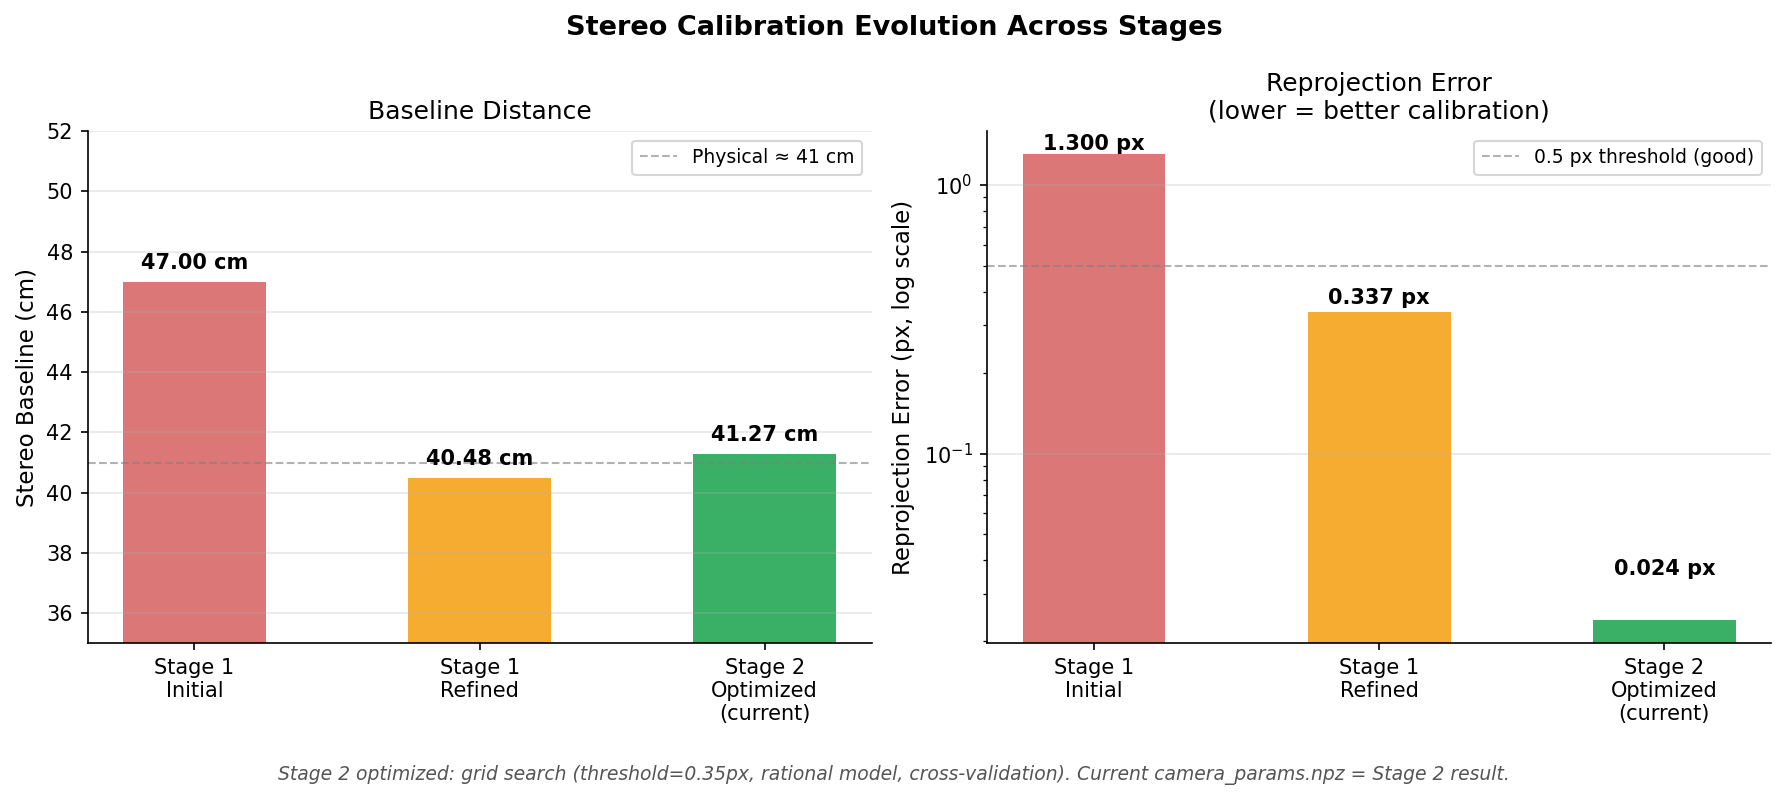
\includegraphics[width=\linewidth]{calibration_evolution.png}
  \caption{Stereo calibration evolution. The current calibration balances a realistic baseline estimate with a low reprojection error, making it suitable as the fixed geometric input for SKT.}
  \label{fig:calibration_evolution}
\end{figure}

\subsection{2025 Ergonomics Dataset}

All quantitative results in this thesis are computed on a single
single-subject ergonomics recording collected in a controlled
manufacturing-like environment, and this is therefore the dominant
generalisability limitation of the present study.
The subject performs a representative mix of factory-floor activities --
walking, sitting, squatting, reaching, lifting, and interacting with
furniture -- so that all major upper- and lower-body postures are exercised
within a single contiguous take rather than as isolated short clips.
After left--right pairing by hardware frame identifier, the usable
synchronised camera timeline contains 2801 frame pairs spanning 248.8\,s,
which corresponds to an effective frame rate of 12.5\,fps; the left raw
metadata contains 3015 rows and the right raw metadata contains 2882 rows,
so a non-trivial fraction of each side is either unpaired or falls outside
the synchronised interval, which is exactly what motivates the explicit
hardware-ID re-pairing step rather than reliance on raw row indices.
Table~\ref{tab:timeline_summary} summarises the resulting working timeline
that all downstream evaluations share.

\begin{table}[!htbp]
  \centering
  \caption{Summary of the synchronized camera timeline used for evaluation.}
  \label{tab:timeline_summary}
  \begin{tabular}{lc}
    \toprule
    Quantity & Value \\
    \midrule
    Synchronized frame pairs & 2801 \\
    Duration & 248.8 s \\
    Median frame interval & 0.0800 s \\
    Effective frame rate & 12.50 fps \\
    Left metadata rows & 3015 \\
    Right metadata rows & 2882 \\
    Rotation applied & 180\degr \\
    \bottomrule
  \end{tabular}
\end{table}

\subsection{Xsens Reference Data and Angle Representations}

The Xsens recording supplies full-body motion data on an independent time
axis and contains two distinct angle representations that the thesis must
choose between before any cross-method comparison can be reported.
The first is the \emph{Xsens native} joint-angle output, which is read
directly from the MVNX joint-angle channels and follows the Xsens body
model together with its internal axis and zero conventions.
The second is the \emph{Xsens-derived geometric} angle representation, in
which the joint angles are re-computed from the Xsens 3D segment positions
using the same three-point arccosine formula that is later applied to the
vision pipelines; this representation is adopted as the main reference
throughout the thesis because it removes the angle-definition mismatch
between the reference and the vision methods at the cost of being a
slightly less direct read of the Xsens body model.

The comparison between the two Xsens representations is then re-used as a
quantitative reference-system sanity check rather than discarded.
At the elbow, the two representations agree to within approximately
1--1.5\degr\ MAE in absolute angle space, and they agree to a Pearson
correlation of $\sim$0.99 in K-frame motion space; at the shoulder and hip,
the agreement is visibly weaker because the underlying axis conventions
differ more.
The implication for the thesis evaluation design is two-fold.
First, the elbow numbers serve as a \emph{lower-bound anchor}: a vision
method whose absolute angle MAE against Xsens-derived geometric is several
times the elbow self-consistency floor is unlikely to be limited by the
reference, whereas one that approaches the floor is approaching the
information limit of the reference itself.
Second, the larger shoulder/hip mismatch is one of the reasons the thesis
reports motion-space metrics alongside absolute angle MAE, since
differencing cancels both the unknown global Xsens calibration offset and
much of the axis-definition mismatch between the two representations.

\subsection{Cross-system Time Synchronisation}

Cross-system synchronisation is unavoidable for the present setup because
the cameras and the Xsens suit run on independent clocks, and any
mis-alignment converts directly into degraded motion-space agreement, so
the thesis adopts an automatic three-score offset search rather than a
manually picked shift.
The procedure first sweeps the offset coarsely between 0 and 30\,s, then
refines around the best candidate; at every candidate it computes three
independent agreement scores -- a position-space score on the 3D segment
positions, an angle-space score on the joint angles, and a motion-delta
score on the K-frame angle deltas -- and selects the motion-delta optimum
as the final offset because the motion evaluation is the most sensitive of
the three to residual sub-second mis-alignment.

For the present recording, the selected offset is 17.31\,s, and the
position-, angle-, and motion-delta optima fall at 17.27\,s, 17.28\,s, and
17.31\,s respectively.
The fact that three scores derived from three independent error spaces
converge inside a window of about 0.04\,s is the strongest evidence
available in this thesis that a single constant offset is an adequate
alignment model for this recording: had the underlying clock relation been
non-constant, the three scores would not be expected to peak so close
together.
Figure~\ref{fig:offset_search} shows the score curves produced by the
search and visualises this triple agreement.

\begin{figure}[!htbp]
  \centering
  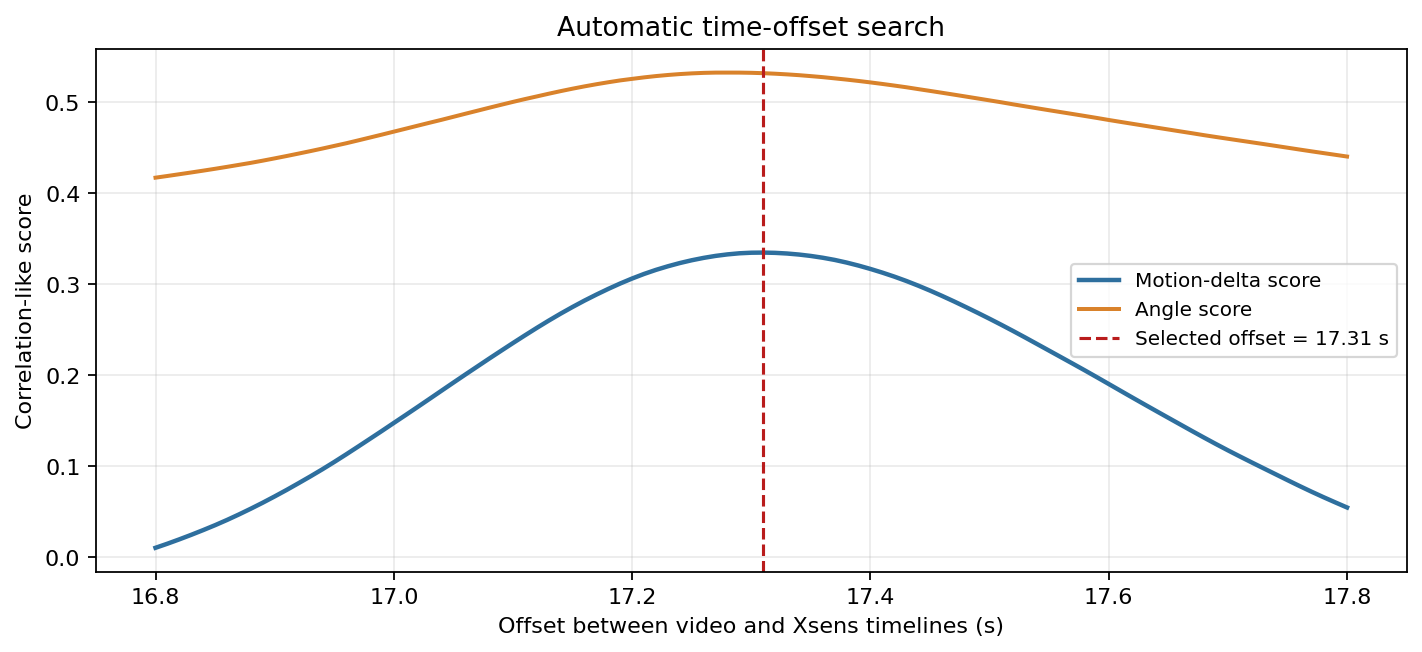
\includegraphics[width=\linewidth]{thesis_offset_search.png}
  \caption{Automatic offset estimation between the camera timeline and the Xsens reference timeline. The final selected value is 17.31 s, with position-, angle-, and motion-based scores all supporting a similar alignment.}
  \label{fig:offset_search}
\end{figure}

A second, qualitative synchronisation check is provided by overlaying the
aligned elbow-angle curves from all systems on the shared timeline
(Figure~\ref{fig:angle_time_alignment}).
The purpose of this plot is not to rank methods at the angle level -- that
is the task of Section~\ref{sec:results} -- but to confirm that the main
movement phases of the recording line up across systems after the offset
has been applied, so that any residual short-term deviation can be
attributed to true method behaviour rather than to an unfixed global shift.

\begin{figure}[!htbp]
  \centering
  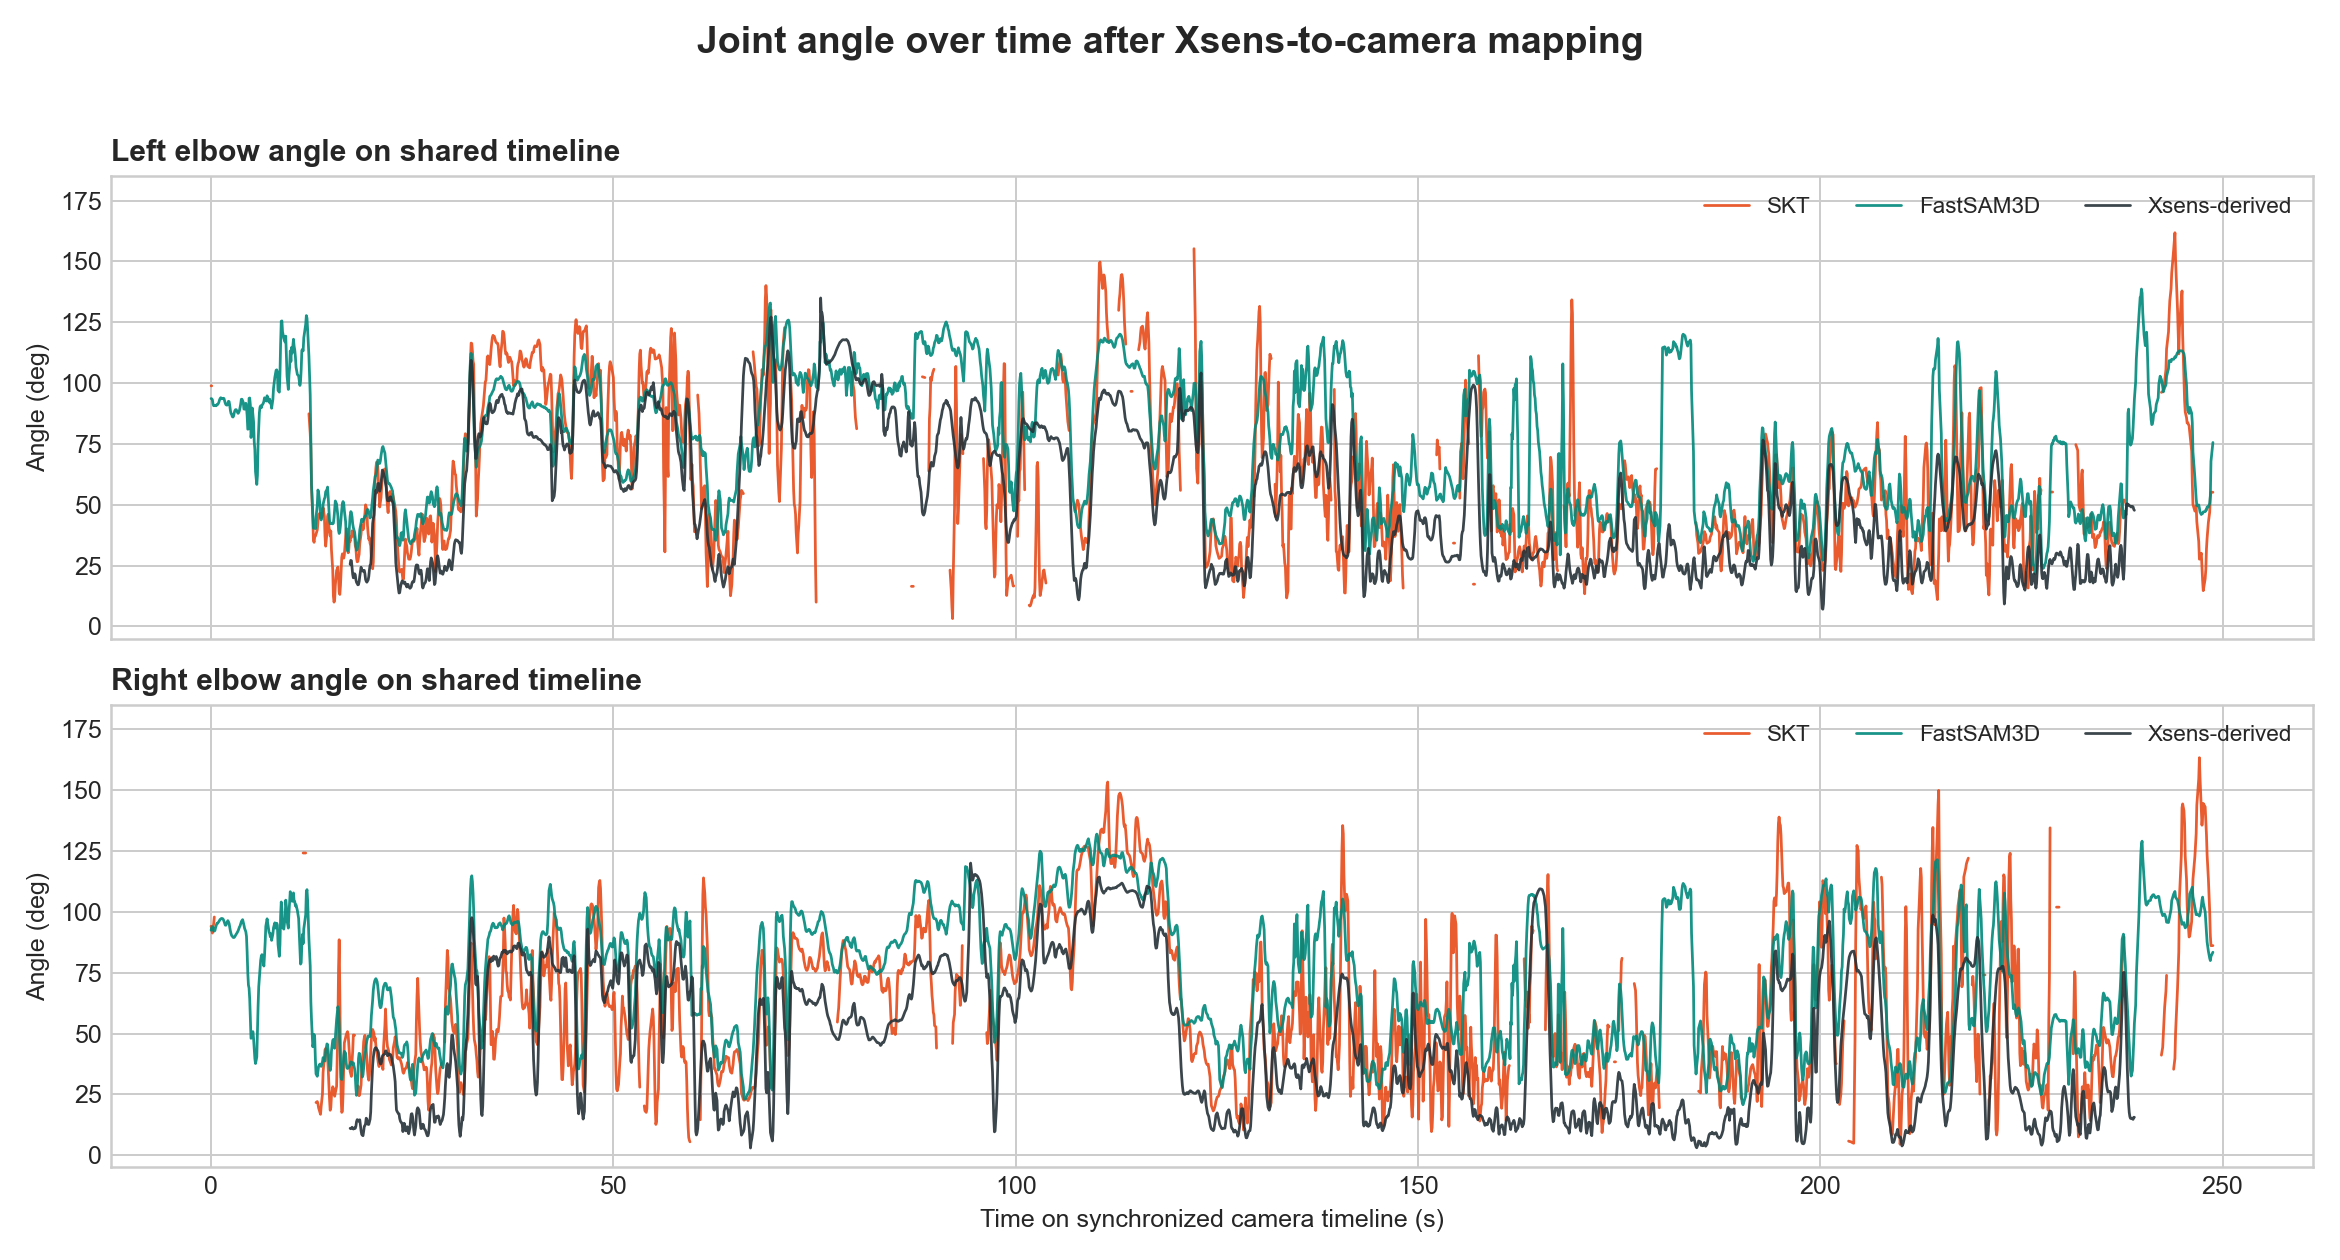
\includegraphics[width=\linewidth]{thesis_joint_angle_over_time.png}
  \caption{Left and right elbow angles on the shared timeline after offset correction. The plot provides a qualitative synchronisation check before quantitative angle and motion metrics are interpreted.}
  \label{fig:angle_time_alignment}
\end{figure}

A third check addresses the possibility that, even with a near-perfect
mean offset, the camera and Xsens clocks could drift slowly over the
$\sim$4\,min recording.
Figure~\ref{fig:first_last_delta} compares the K=6 motion-delta windows at
the beginning and end of the common valid interval; had the underlying
drift been large, the late-interval deltas would be expected to lose their
alignment with the reference even though the early-interval deltas still
agree.
The check is qualitative rather than a formal drift estimate, but the
observed late-interval agreement is comparable to the early-interval
agreement, which supports the use of a single constant offset for the
remainder of the thesis while explicitly acknowledging that future longer
or multi-take recordings should repeat this check.

\begin{figure}[!htbp]
  \centering
  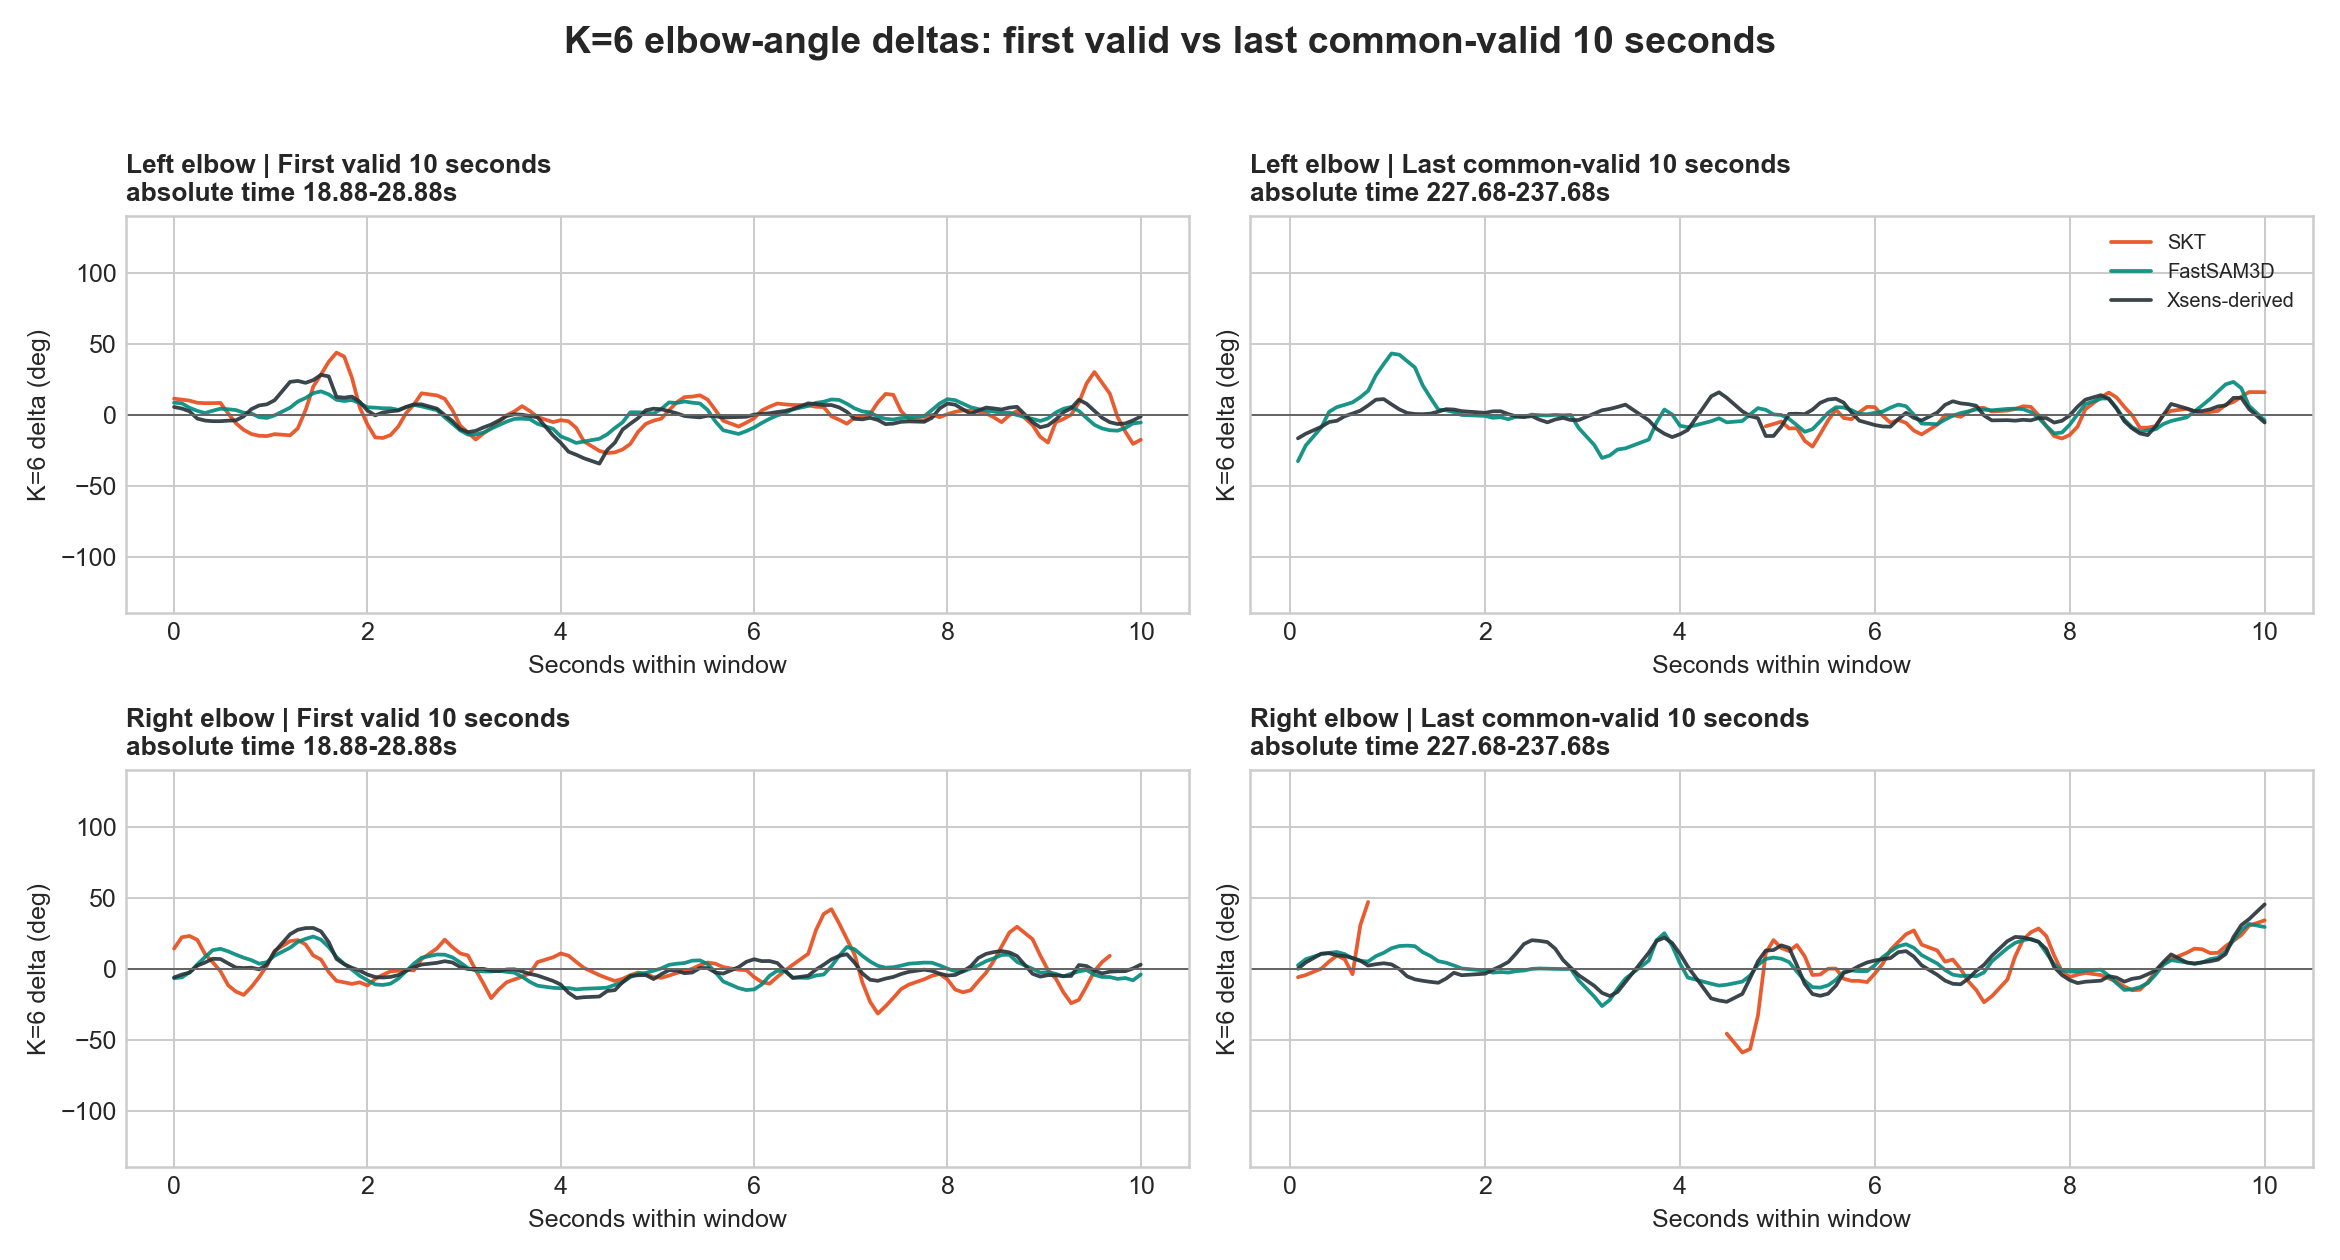
\includegraphics[width=\linewidth]{thesis_k6_delta_first_last_10s.png}
  \caption{K=6 elbow motion deltas near the beginning and end of the common valid interval. This figure is used as a practical check that the chosen constant offset remains reasonable across the recording.}
  \label{fig:first_last_delta}
\end{figure}

\clearpage
% =============================================================
\section{Methods}
\label{sec:methods}
% =============================================================

\subsection{Overview}

The thesis benchmarks two pose-estimation pipelines against the same Xsens
reference and the same evaluation protocol: SKT, the primary calibrated
sparse-stereo method developed in this thesis, and FastSAM3D, the monocular
learning-based alternative.
Figure~\ref{fig:pipeline_overview} shows the full experimental flow, and
Table~\ref{tab:method_roles} summarises each pipeline's input assumption, main
advantage, and main risk.

The single design choice that matters most for interpreting the rest of the
thesis is the deliberate separation between pose estimation and evaluation.
Both methods are mapped onto the same shared timeline and judged with
the same metrics, but those metrics are then split across two independent
axes (angle, motion) rather than collapsed into a single ranking
score; this prevents the recurring failure mode in which a method that is
strong in one space, for example metric stereo geometry, is implicitly
assumed to be equally strong in temporal angle consistency.

\begin{figure}[!htbp]
  \centering
  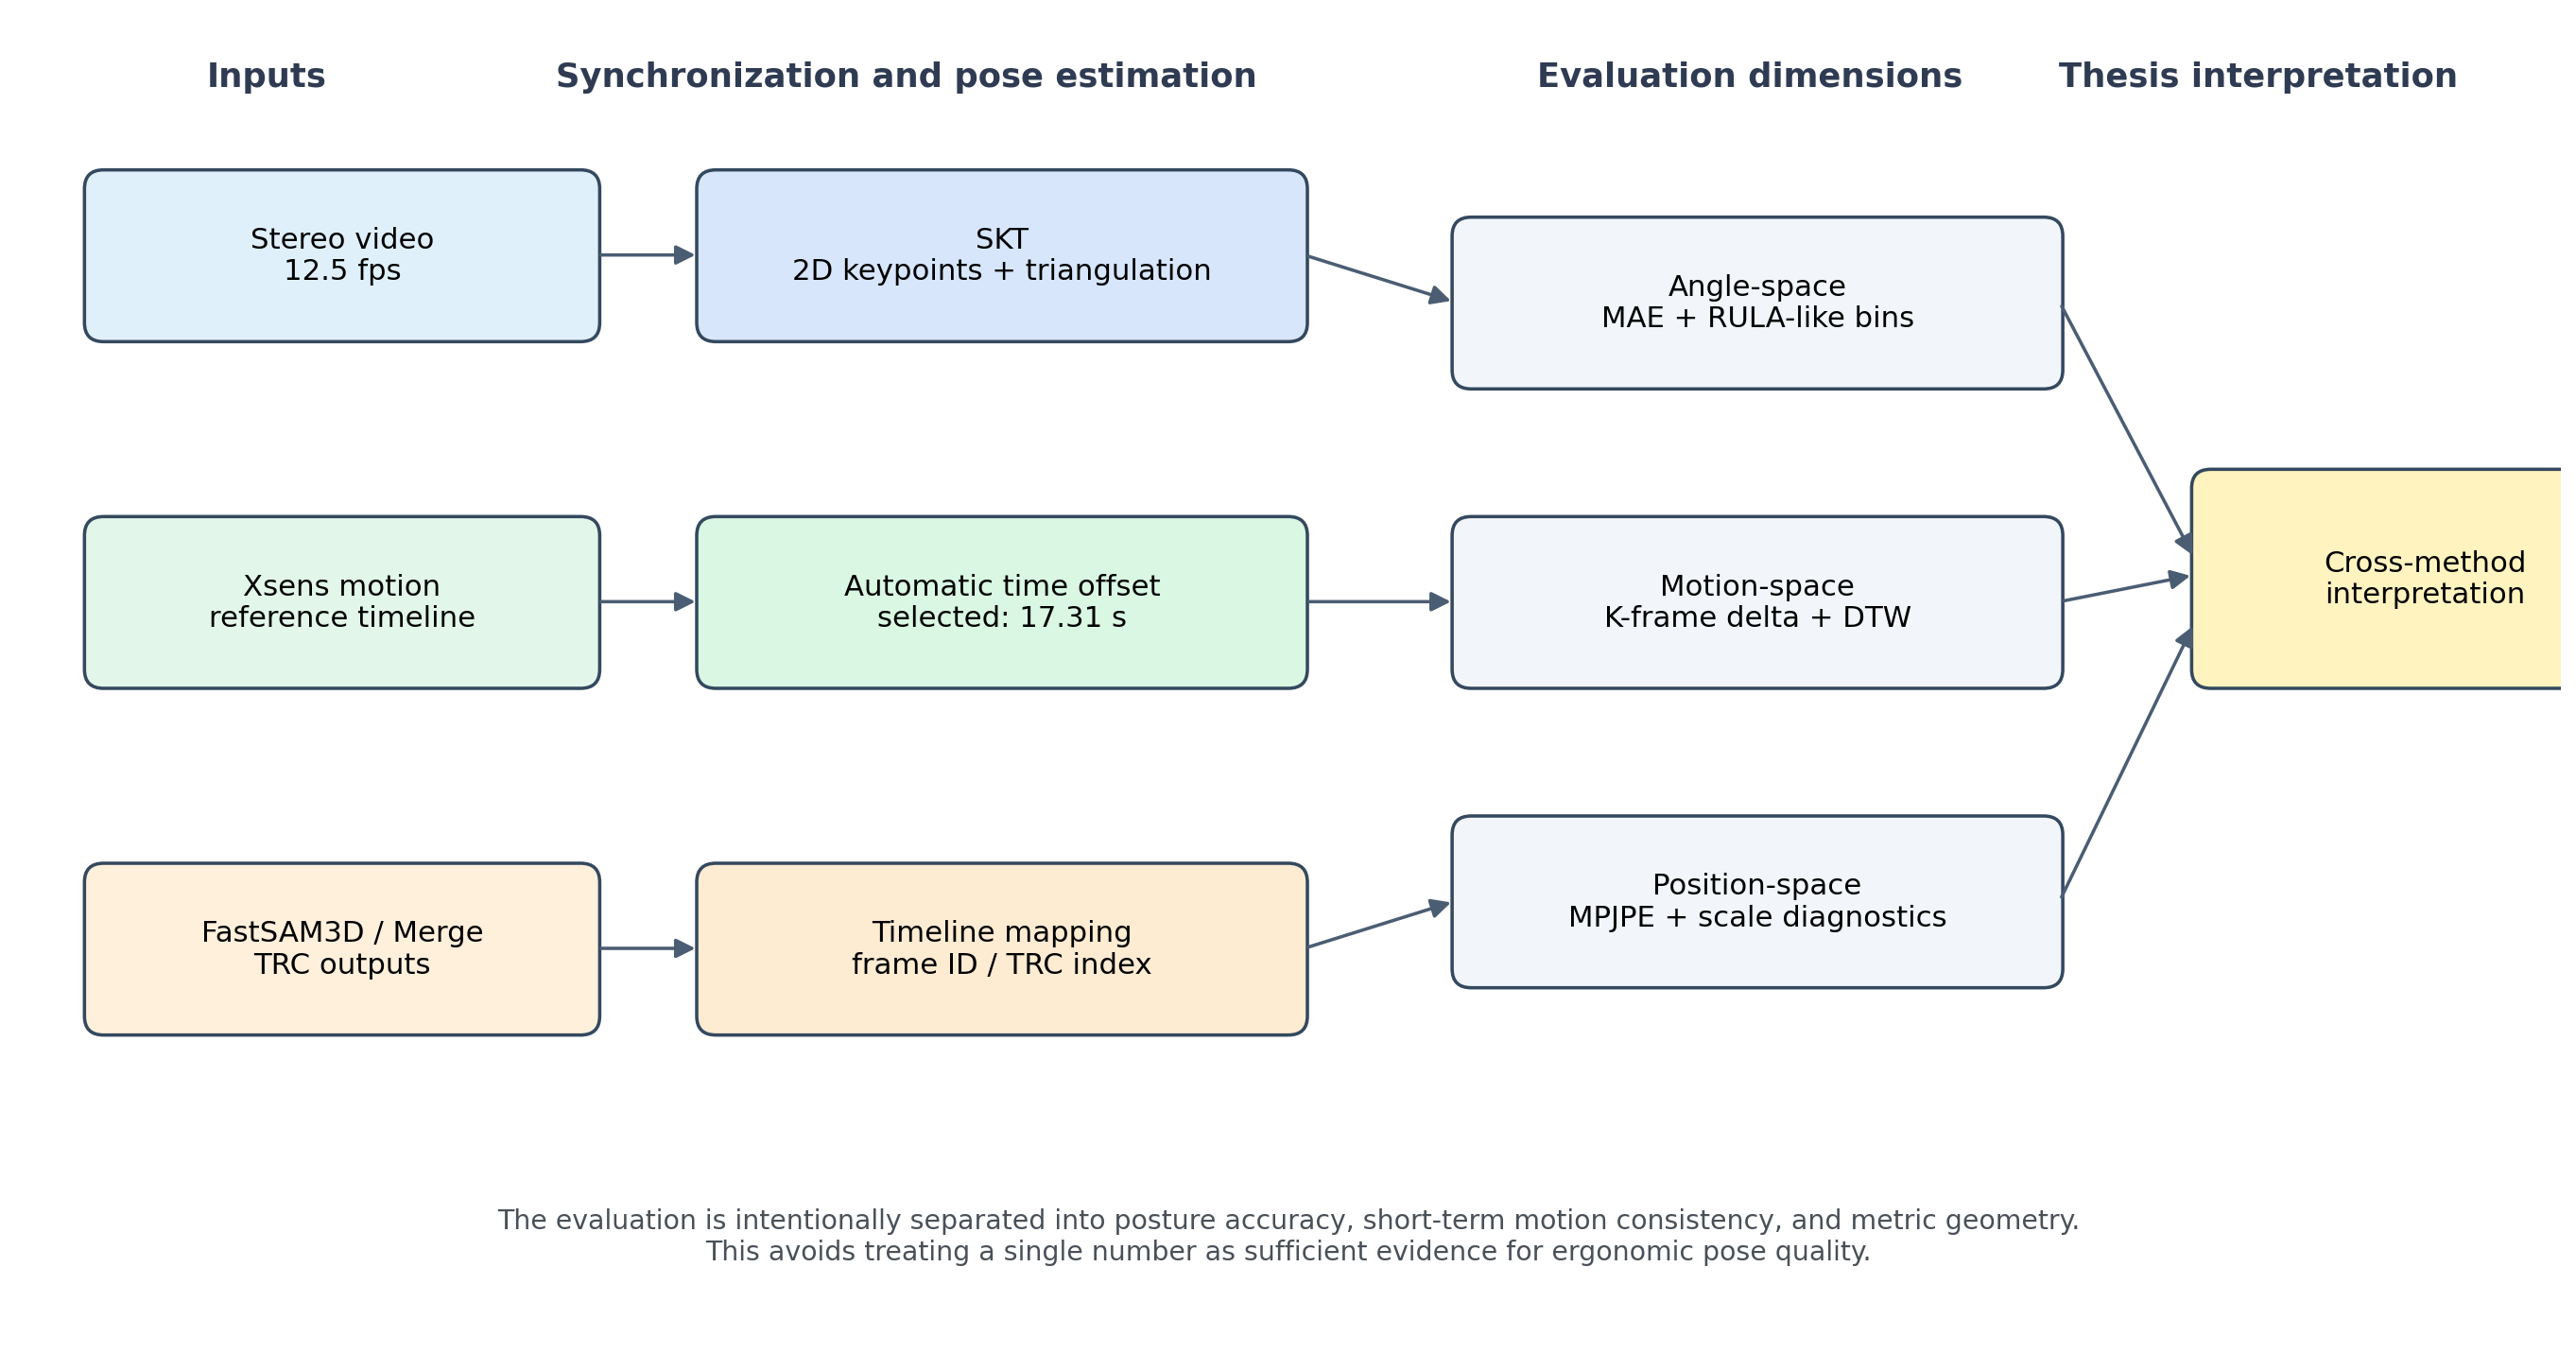
\includegraphics[width=\linewidth]{thesis_pipeline_overview.png}
  \caption{Overview of the thesis evaluation pipeline. Inputs are synchronized and evaluated separately in angle space, motion space, and position space before the final cross-method interpretation.}
  \label{fig:pipeline_overview}
\end{figure}

\begin{table}[!htbp]
  \centering
  \caption{Role of each evaluated pose-estimation path in the thesis.}
  \label{tab:method_roles}
  \small
  \begin{tabularx}{\linewidth}{lXXX}
    \toprule
    Method & Input assumption & Main advantage & Main risk \\
    \midrule
    SKT
    & Synchronized stereo video and calibrated cameras
    & Metric 3D scale and explicit geometric quality signals
    & 2D keypoint jitter and left--right mismatch are amplified by triangulation \\
    FastSAM3D
    & Monocular pose output provided as TRC markers
    & Learned body/motion priors give stable angle and motion behaviour
    & Coordinate, scale, and keypoint semantics require careful interpretation \\
    \bottomrule
  \end{tabularx}
\end{table}

\subsection{Sparse Keypoint Triangulation (SKT)}

The primary method developed in this thesis, Sparse Keypoint Triangulation
(SKT), turns a calibrated stereo video pair into a 3D body skeleton through
a transparent geometric chain that exposes per-frame quality signals at
every stage.
For each synchronised left/right frame pair, the pipeline first runs a 2D
human pose detector on each view to obtain 17 COCO-format keypoints with
per-keypoint confidence; the two views' keypoints are then matched by
keypoint index and filtered by three geometric consistency checks
(minimum triangulation confidence, maximum epipolar error, maximum
reprojection error after triangulation); the surviving pairs are
triangulated into 3D coordinates through the Direct Linear Transform
applied to the calibrated projection matrices; and finally the joint
angles are computed from triplets of 3D keypoints using the same
three-point arccosine formula that is applied to the Xsens-derived
geometric reference.

The methodological reason for building SKT this way -- rather than, for
example, regressing 3D pose directly with a learned model -- is
interpretability under deployment.
Every 3D point in an SKT output is tied to two observed 2D detections and
to a known stereo calibration model, so the pipeline can expose a set of
geometry-aware quality signals (triangulation confidence, epipolar error,
reprojection error, disparity) that downstream ergonomic monitoring can
use as a per-frame trust score; unreliable frames can therefore be
detected and gated rather than silently converted into ergonomic risk
scores, which is a property no end-to-end learned regressor offers for
free.
The corresponding methodological cost is that each SKT 3D point inherits
the noise of its 2D detections in both views; small 2D jitter is first
amplified by triangulation and then further amplified by joint-angle
computation, so SKT is most usefully understood as a measurement pipeline
whose output should be read together with its quality signals rather than
as a smoothed motion sequence.

This view of SKT as a measurement pipeline -- rather than a black-box
reconstruction module -- is also what motivates the later motion-delta
evaluation.
When a wrist or elbow keypoint is detected inconsistently between the two
views, the resulting 3D joint can remain numerically valid (the rays still
intersect, the reprojection is still small) while producing a sharply
different triangulated angle from the surrounding frames, which appears in
later analysis as occasional large motion deltas concentrated near
elbow-chain instabilities.
Section~\ref{sec:discussion} returns to these high-delta cases as concrete
failure evidence rather than treating them as generic noise.

\subsection{FastSAM3D (Monocular Learning Baseline)}

FastSAM3D is included as the learning-based monocular counterpart to SKT
and is the most informative single comparison in the thesis, because it
keeps the same input modality (the camera) but replaces multi-view
geometry with learned body-shape and motion priors.
Instead of triangulating left/right keypoint pairs, FastSAM3D produces a
3D pose directly from one camera stream through a model-based pipeline
that combines fast instance segmentation with learned body-shape and pose
priors \cite{yang2026fastsam3d}; the specific FastSAM3D
implementation is treated here as an externally produced output, and its
results are delivered as TRC marker files that are re-mapped to the
COCO-17 keypoint convention and resampled onto the shared camera timeline
before any evaluation metric is computed.

The methodological reason to include FastSAM3D is that learned body-shape
and motion priors should, in principle, smooth out the per-frame keypoint
noise that hurts SKT, because the learned model implicitly enforces
anatomically consistent transitions between consecutive poses even without
explicit multi-view evidence.
The corresponding methodological cost is that the FastSAM3D output does
not necessarily share the SKT coordinate frame, scale convention, or
exact keypoint semantics; FastSAM3D is therefore evaluated primarily in
the angle and motion axes, where these conventions cancel, while
position-space results are reported only as coordinate/scale diagnostics
rather than as direct pose-quality scores.

\clearpage
% =============================================================
\section{Evaluation Framework}
\label{sec:evaluation}
% =============================================================

\subsection{Angle-space Evaluation}

The angle-space track answers the most direct question for ergonomic
deployment -- ``Is the estimated joint posture quantitatively close to
the reference?'' -- and it is therefore reported first in every per-method
analysis even though it is the axis most exposed to the Xsens calibration
limitation discussed in Section~\ref{sec:background}.
Eight full-body angles are evaluated, covering the four bilateral joints
that drive most of the RULA assessment: left and right shoulder, elbow,
hip, and knee flexion.
To remove angle-definition mismatch between systems, every angle is
computed from the same three-point geometric formula applied to the
relevant triplet of 3D keypoints, both for the vision methods and for the
Xsens-derived geometric reference:
\begin{equation}
  \theta = \arccos\!\left(
    \frac{(\mathbf{p}_A-\mathbf{p}_B)\cdot(\mathbf{p}_C-\mathbf{p}_B)}
         {\|\mathbf{p}_A-\mathbf{p}_B\|\;\|\mathbf{p}_C-\mathbf{p}_B\|}
  \right).
\end{equation}
The main reported metrics are mean absolute error (MAE), median absolute
error, bias (signed mean error), valid-pair ratio, and -- as the
application-level companion -- RULA-like bin agreement for the
upper-body joints.

\subsection{Motion-space Evaluation}

The motion-space track is the thesis's principal countermeasure against
the Xsens calibration offset: it asks whether two systems describe the
\emph{same change in posture} rather than the same absolute posture, so
that any static reference offset cancels out by differencing.
For a given time scale $K$, the K-frame angle delta is defined as
\begin{equation}
  \Delta_K \theta_t \;=\; \theta_t \;-\; \theta_{t-K},
\end{equation}
and the thesis evaluates four time scales, $K\in\{1,6,12,25\}$ frames
(approximately 0.08, 0.48, 0.96, and 2.00\,s at 12.5\,fps), to probe the
agreement across genuinely instantaneous changes, sub-second sub-actions,
1\,s smooth-motion windows, and 2\,s near-action-level windows.
K=6 is adopted as the main reporting and visualisation scale because it
corresponds to a $\sim$0.48\,s sub-action -- short enough to remain a
true motion-level metric, long enough to suppress per-frame keypoint
jitter -- while the K=1 and K=25 numbers provide context as the
noise-dominated and amplitude-dominated extremes.
Reported metrics include Pearson correlation, Spearman rank correlation,
delta MAE and RMSE, high-delta count, and the path ratio (cumulative
absolute target delta divided by cumulative absolute reference delta),
which together separate ``shape agreement'' from ``amplitude agreement''
in the motion signal.

\subsection{Segment-level Evaluation}

The segment-level track condenses the frame-level motion comparison into
a small set of physically interpretable active-movement intervals,
because reporting only frame-level metrics tends to hide whether a method
captures the actual movement bursts that ergonomic risk assessment cares
about.
Activity segments are detected from the reference signal as contiguous
intervals of sustained K-frame motion above a threshold, and for each
segment four numbers are reported per method: range of motion (ROM,
max-min angle), per-segment angle MAE, RULA-like bin agreement based on
the segment's peak angle, and a dynamic time warping (DTW) distance
\cite{sakoe1978dtw}.
The DTW comparison is run on \emph{mean-subtracted and L2-normalised}
per-segment angle sequences, following the practice that has been
recommended for human-motion shape comparison in the recent literature
\cite{perezluque2026reaching}; the normalisation deliberately removes
absolute offset and amplitude so that DTW measures whether the
\emph{shape of motion through the segment} is similar, making it
complementary to MAE/RMSE (which measure amplitude error) rather than
redundant with them.

\subsection{Position-space Evaluation}

The position-space track does not compete with the angle and motion
tracks for ``best pose method'' -- it answers a separate deployment
question: ``Which method produces 3D coordinates whose scale and
geometry can be trusted in a metric workspace?''
For SKT, calibrated stereo geometry gives the coordinates an inherent
metric scale, so MPJPE-style distances and pelvis-relative comparisons
can be reported directly after rigid alignment using the standard Kabsch
estimator \cite{kabsch1976solution}.
For FastSAM3D, the output coordinate frame and scale convention do not
necessarily match the stereo or Xsens frames, so position-space numbers
must be reported with explicit alignment provenance; the thesis uses
position-space results primarily to (i) demonstrate stereo's
metric-scale advantage and (ii) document the coordinate/scale work that
any monocular pipeline must do before its 3D output becomes deployable.

\subsection{Filtering Policy}

The evaluation tracks above are well-defined only if the per-system
filtering policy is itself controlled, because temporal smoothing
applied at different strengths to different systems can quietly inflate
or deflate motion-space agreement without changing any reported number
in an obvious way.
The thesis therefore adopts a deliberate per-system policy.
Xsens streams are interpolated onto the shared timeline but are
\emph{not} re-smoothed by the project, because the Xsens internal
processing already includes substantial filtering, and stacking a
project-side filter on top would silently double the smoothing on
the reference side of every comparison.
The camera-based methods are smoothed with a single light moving-average
filter whose window is recorded in the run configuration; the chosen
window represents a $\sim$200\,ms low-lag setting consistent with empirical
guidance for human upper-body motion signals \cite{perezluque2026reaching}.
The single methodological invariant that must hold across all runs is
that smoothing is always applied \emph{before} delta computation, since
the opposite order would let the delta metric measure filter artifacts
rather than the underlying motion signal.

\begin{table}[!htbp]
  \centering
  \caption{Interpretation of the evaluation tracks used in the thesis.}
  \label{tab:evaluation_tracks}
  \small
  \begin{tabularx}{\linewidth}{lXXX}
    \toprule
    Track & Question answered & Main metrics & Main caveat \\
    \midrule
    Angle-space
    & Is the posture suitable for ergonomic angle interpretation?
    & MAE, median AE, bias, valid ratio, RULA-like bin agreement
    & Sensitive to reference-system angle definitions and static offsets \\
    Motion-space
    & Do two systems describe the same short-term movement?
    & K-frame delta correlation, delta MAE, RMSE, high-delta count, DTW
    & Requires careful time alignment and consistent smoothing policy \\
    Segment-level
    & Are active movement intervals similar in range and shape?
    & ROM error, segment MAE, DTW distance, RULA-like agreement
    & Depends on segment detection thresholds and valid-frame coverage \\
    Position-space
    & Are reconstructed 3D skeletons geometrically compatible?
    & MPJPE, pelvis-relative distance, aligned inter-method distance
    & Monocular methods may use different coordinate and scale conventions \\
    \bottomrule
  \end{tabularx}
\end{table}

This separation is central to the thesis argument.
For example, a method can produce good angle trends while still being
difficult to compare in absolute 3D coordinates, or it can preserve metric
scale while producing jittery short-term angles.
The evaluation framework therefore reports multiple complementary quantities
instead of selecting a single ``winner'' metric.

\clearpage
% =============================================================
\section{Results}
\label{sec:results}
% =============================================================

\subsection{Angle-space Results}

In the angle-space track, the monocular learning-based FastSAM3D pipeline
outperforms SKT, but the margin is small enough that the result must be
read with the Xsens reference-system caveat in mind rather than as a
universal verdict.
Averaged across the eight evaluated joint angles, FastSAM3D reaches a mean
MAE of 15.4\degr\ against the Xsens-derived reference, compared with
17.6\degr\ for SKT; the corresponding median MAEs (14.4\degr\ vs.\
17.9\degr) preserve the same ranking, and FastSAM3D also has the higher
valid-pair ratio (0.905 vs.\ 0.746).
The Xsens-native check sits at 4.7\degr\ MAE, an order of magnitude below
the vision methods, and is reported in the same table only as a
reference-system internal anchor rather than as a competing pose method.

The most informative joint-level pattern is that the per-joint MAE
ranking is not flat across the eight angles.
Shoulder, hip, and knee angles dominate FastSAM3D's lead, where its
learned body priors stabilise the chain endpoints; the elbow is the
hardest joint for every vision method, in line with the long
shoulder--elbow--wrist chain that amplifies both keypoint noise (for SKT)
and pose-prior uncertainty (for FastSAM3D), and this is the joint where
both methods are penalised most by the Xsens calibration offset
itself.
For this reason the elbow is the joint that drives the motion-space
analysis that follows -- angle MAE alone cannot tell which fraction of
the elbow error is genuine pose error and which fraction is reference
offset.

\begin{table}[!htbp]
  \centering
  \caption{Angle-space summary across eight evaluated joint angles. Lower MAE is better.}
  \label{tab:angle_summary}
  \small
  \begin{tabular}{lcccc}
    \toprule
    Method & Mean MAE $\downarrow$ & Median MAE $\downarrow$ &
    Valid ratio $\uparrow$ & Bin agreement $\uparrow$ \\
    \midrule
    SKT & 17.6 & 17.9 & 0.746 & 0.540 \\
    \good{FastSAM3D} & \good{15.4} & \good{14.4} & \good{0.905} & \good{0.553} \\
    \textit{Xsens native check} & \textit{4.7} & \textit{3.7} & \textit{0.905} & \textit{0.886} \\
    \bottomrule
  \end{tabular}
\end{table}

Figure~\ref{fig:angle_summary_plot} visualises the same comparison.
The bar plot is included precisely because the FastSAM3D--SKT gap is
small and consistent rather than large and dramatic; a single bar
that was twice as high as another would not survive any reasonable
sensitivity check on this single recording, whereas a small but
systematic gap is the more honest evidence on which to base the
discussion of learned pose priors later in the thesis.

\begin{figure}[!htbp]
  \centering
  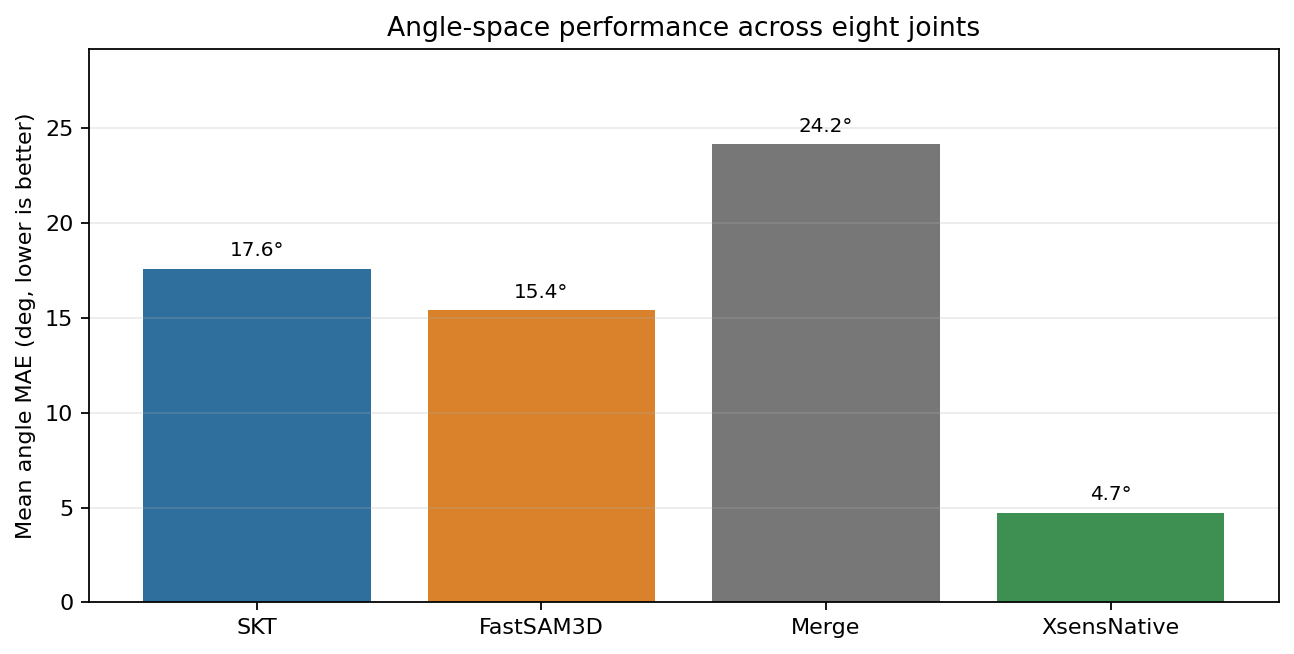
\includegraphics[width=0.92\linewidth]{thesis_angle_summary.png}
  \caption{Angle-space summary across evaluated methods. FastSAM3D has the lowest mean and median MAE among the vision methods, while the Xsens-native check indicates the approximate lower bound of the reference-system representation difference.}
  \label{fig:angle_summary_plot}
\end{figure}

\subsection{Motion-space Results}

In the motion-space track, the FastSAM3D advantage observed in absolute
angles becomes both clearer and easier to interpret, because differencing
the angle sequences cancels the Xsens calibration offset that confounded
the angle-space comparison.
Averaged across the eight evaluated angles at $K=6$ frames ($\sim$0.48\,s),
FastSAM3D reaches a mean Pearson correlation of 0.64 with the Xsens-derived
reference, against 0.38 for SKT; the corresponding mean Spearman rank
correlations (0.64 vs.\ 0.33) preserve the same ranking, which rules out
the explanation that FastSAM3D is winning only because of a handful of
high-amplitude points that inflate Pearson without lifting the rank
correlation.
At the elbow -- the joint that the motion-space track is designed to
adjudicate -- FastSAM3D reaches Pearson correlations of 0.54 (left) and
0.69 (right) against SKT's 0.39 / 0.39, a comparable shape-agreement gap
on the joint that the angle-space analysis flagged as ambiguous.
The Xsens-native check returns the expected $\sim$0.96 mean correlation,
confirming that the K=6 metric can recover near-perfect agreement when
the two compared signals genuinely measure the same motion.

\begin{table}[!htbp]
  \centering
  \caption{K=6 motion-delta agreement. Higher correlation is better.}
  \label{tab:motion_summary}
  \small
  \begin{tabular}{lcccc}
    \toprule
    Method & Mean $r$ $\uparrow$ & Mean $\rho$ $\uparrow$ &
    L-elbow $r$ $\uparrow$ & R-elbow $r$ $\uparrow$ \\
    \midrule
    SKT & 0.379 & 0.334 & 0.392 & 0.386 \\
    \good{FastSAM3D} & \good{0.644} & \good{0.635} & \good{0.542} & \good{0.689} \\
    \textit{Xsens native check} & \textit{0.965} & \textit{0.936} & \textit{0.988} & \textit{0.993} \\
    \bottomrule
  \end{tabular}
\end{table}

Figure~\ref{fig:motion_k6_summary_plot} visualises the K=6 correlation
summary and makes the main finding immediately legible: FastSAM3D is
consistently above SKT across the eight evaluated angles, and the Xsens-native
check provides the visual upper bound that anchors the scale of the plot.
The per-elbow scatter plots in Figure~\ref{fig:k6_elbow_scatter} then make
the same comparison at the frame level rather than the summary level:
FastSAM3D's scatter clusters along the ideal diagonal with limited vertical
spread, whereas SKT's scatter shows a recurring vertical accumulation near
zero reference delta -- the geometric signature of high SKT delta values
during physically quiet intervals, which Section~\ref{sec:discussion}
traces back to localised keypoint-chain instability rather than to a
constant noise floor.

\begin{figure}[!htbp]
  \centering
  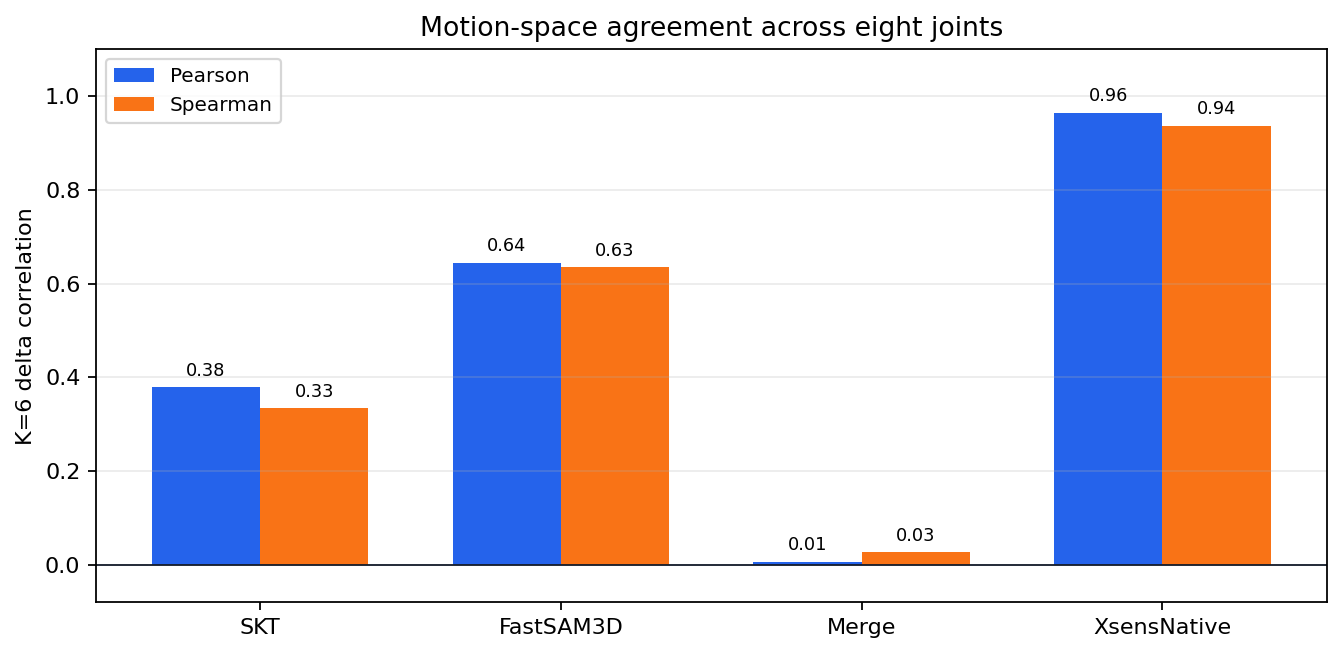
\includegraphics[width=0.92\linewidth]{thesis_motion_k6_summary.png}
  \caption{K=6 motion-delta correlation summary. FastSAM3D shows stronger short-term motion agreement than SKT on the current dataset.}
  \label{fig:motion_k6_summary_plot}
\end{figure}

\begin{figure}[!htbp]
  \centering
  \begin{subfigure}[b]{0.48\linewidth}
    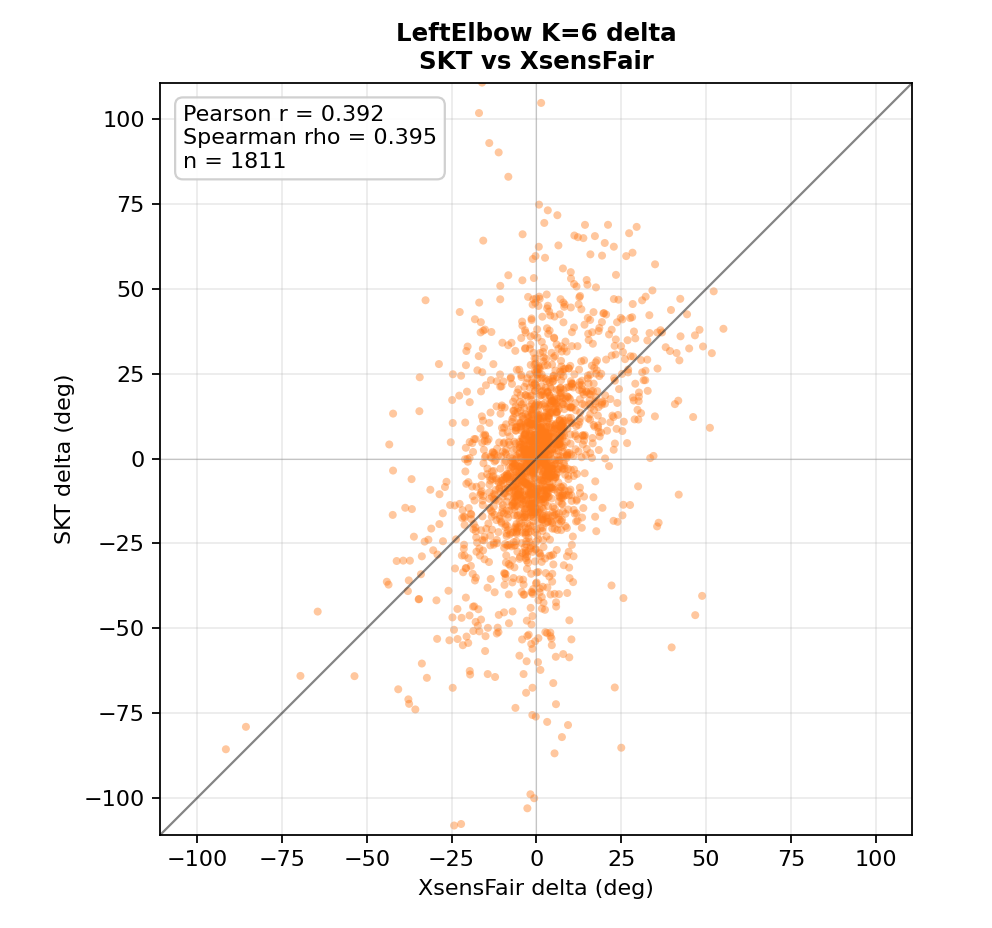
\includegraphics[width=\linewidth]{thesis_scatter_skt_vs_xsensfair_leftelbow_k6.png}
    \caption{SKT, left elbow.}
  \end{subfigure}
  \hfill
  \begin{subfigure}[b]{0.48\linewidth}
    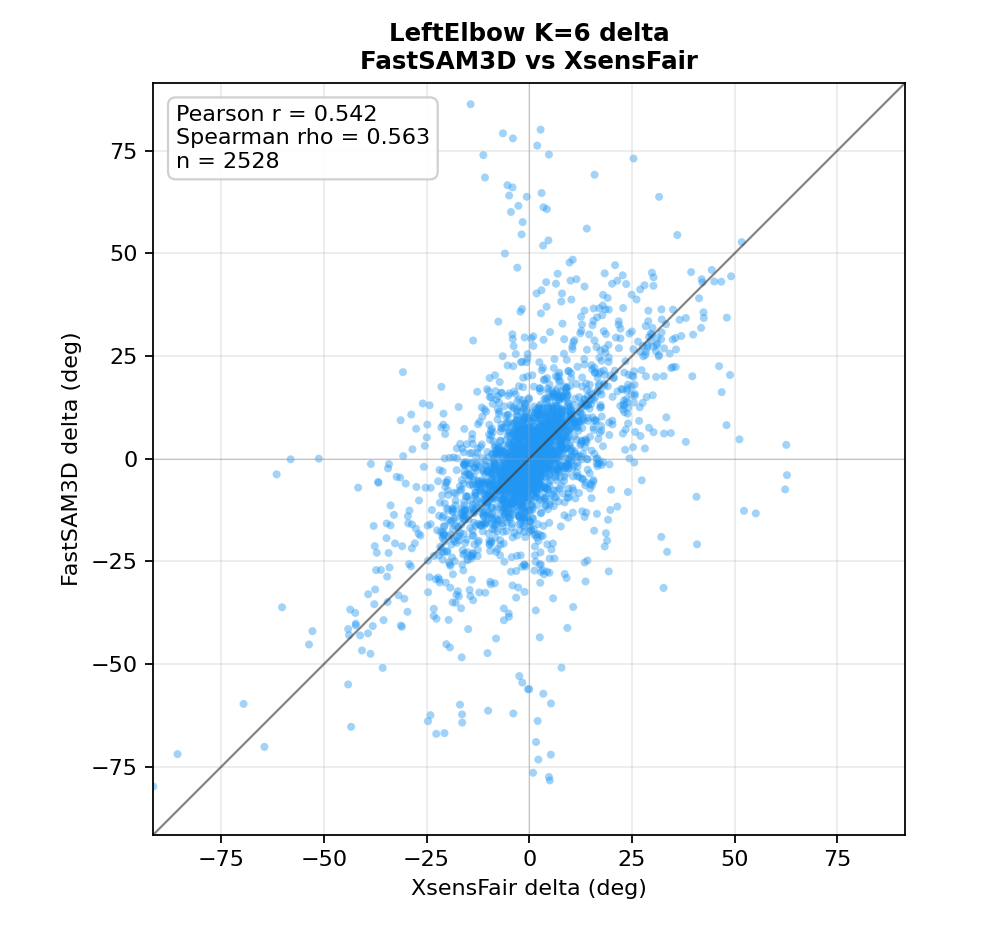
\includegraphics[width=\linewidth]{thesis_scatter_fastsam3d_vs_xsensfair_leftelbow_k6.png}
    \caption{FastSAM3D, left elbow.}
  \end{subfigure}

  \vspace{0.4cm}
  \begin{subfigure}[b]{0.48\linewidth}
    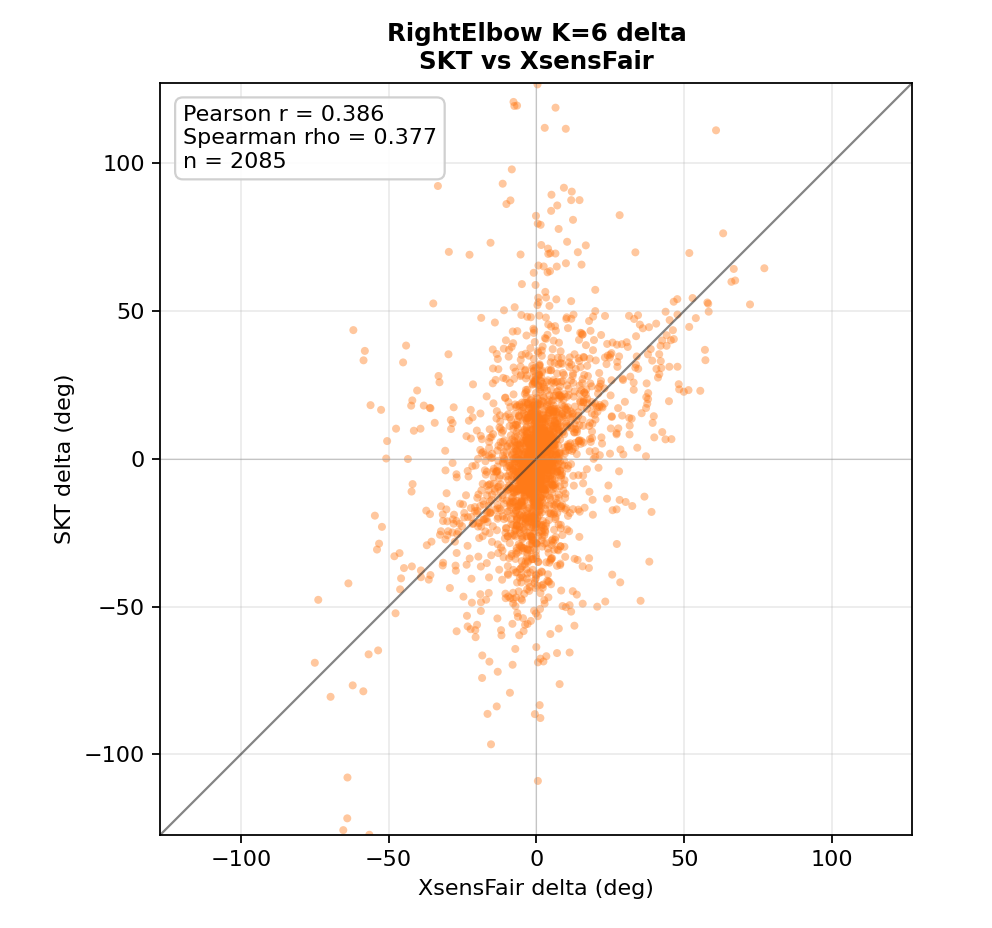
\includegraphics[width=\linewidth]{thesis_scatter_skt_vs_xsensfair_rightelbow_k6.png}
    \caption{SKT, right elbow.}
  \end{subfigure}
  \hfill
  \begin{subfigure}[b]{0.48\linewidth}
    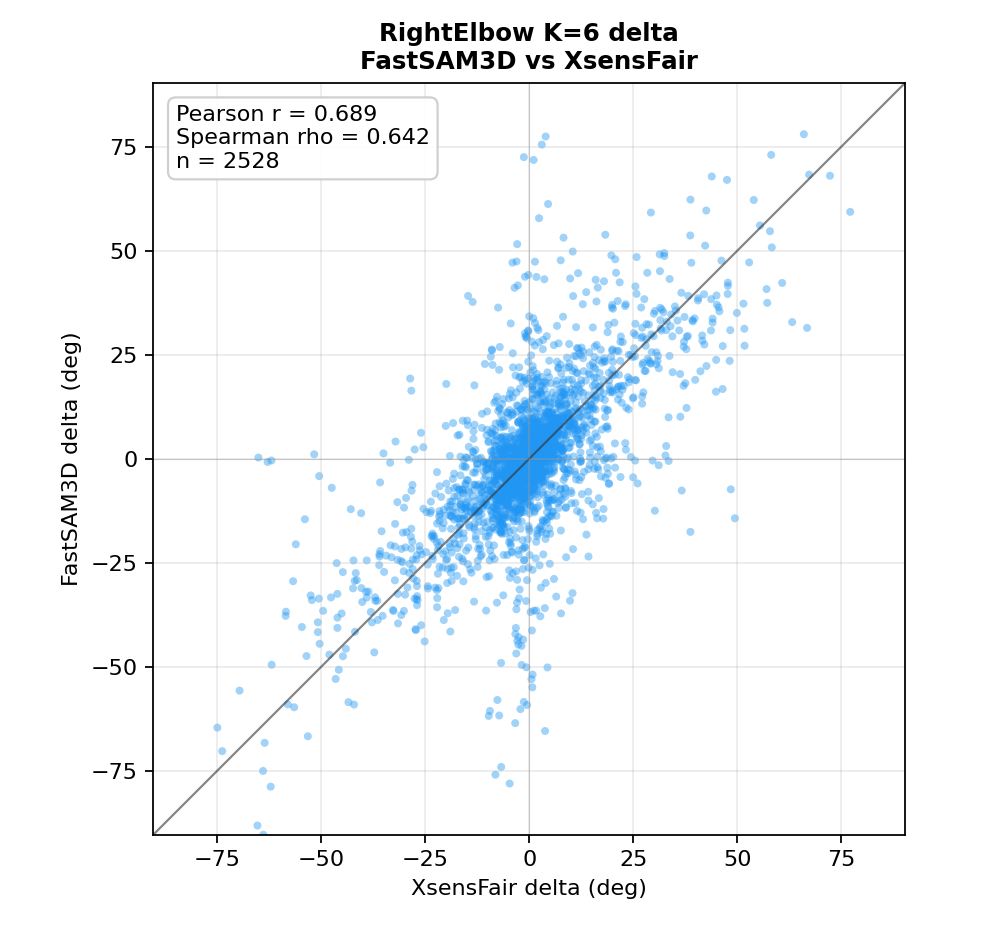
\includegraphics[width=\linewidth]{thesis_scatter_fastsam3d_vs_xsensfair_rightelbow_k6.png}
    \caption{FastSAM3D, right elbow.}
  \end{subfigure}
  \caption{K=6 elbow motion-delta scatter plots against the Xsens-derived reference. FastSAM3D follows the ideal trend more consistently, while SKT shows more high-delta jitter and vertical-axis accumulation.}
  \label{fig:k6_elbow_scatter}
\end{figure}

The sensitivity of the motion-space ranking to the chosen time scale is
shown in Figure~\ref{fig:pearson_vs_k}.
At $K=1$ (single-frame deltas, $\sim$80\,ms) every vision method's
correlation drops because the metric is dominated by per-frame keypoint
jitter that is roughly uncorrelated with the reference; at $K=25$
($\sim$2\,s) every vision method's correlation rises because the metric
is approaching an amplitude-of-motion comparison rather than a true
short-term agreement.
The thesis adopts $K=6$ as the main reporting point because it lies on
the elbow of these two trends: it suppresses single-frame keypoint noise
without smoothing across a complete action, so the ranking it produces
remains a genuine motion-agreement statement rather than either a
noise floor or a re-statement of segment-level ROM.

\begin{figure}[!htbp]
  \centering
  \begin{subfigure}[b]{0.48\linewidth}
    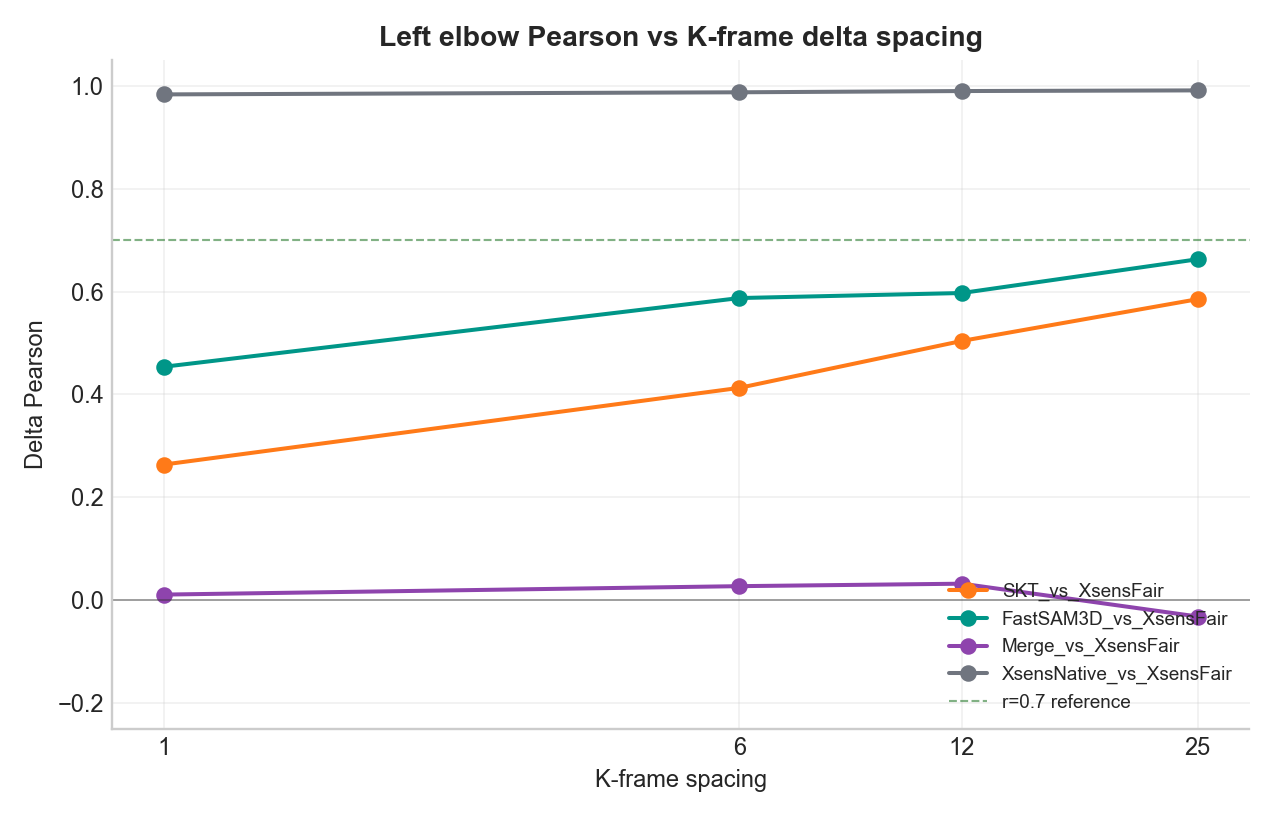
\includegraphics[width=\linewidth]{thesis_pearson_vs_k_leftelbow.png}
    \caption{Left elbow.}
  \end{subfigure}
  \hfill
  \begin{subfigure}[b]{0.48\linewidth}
    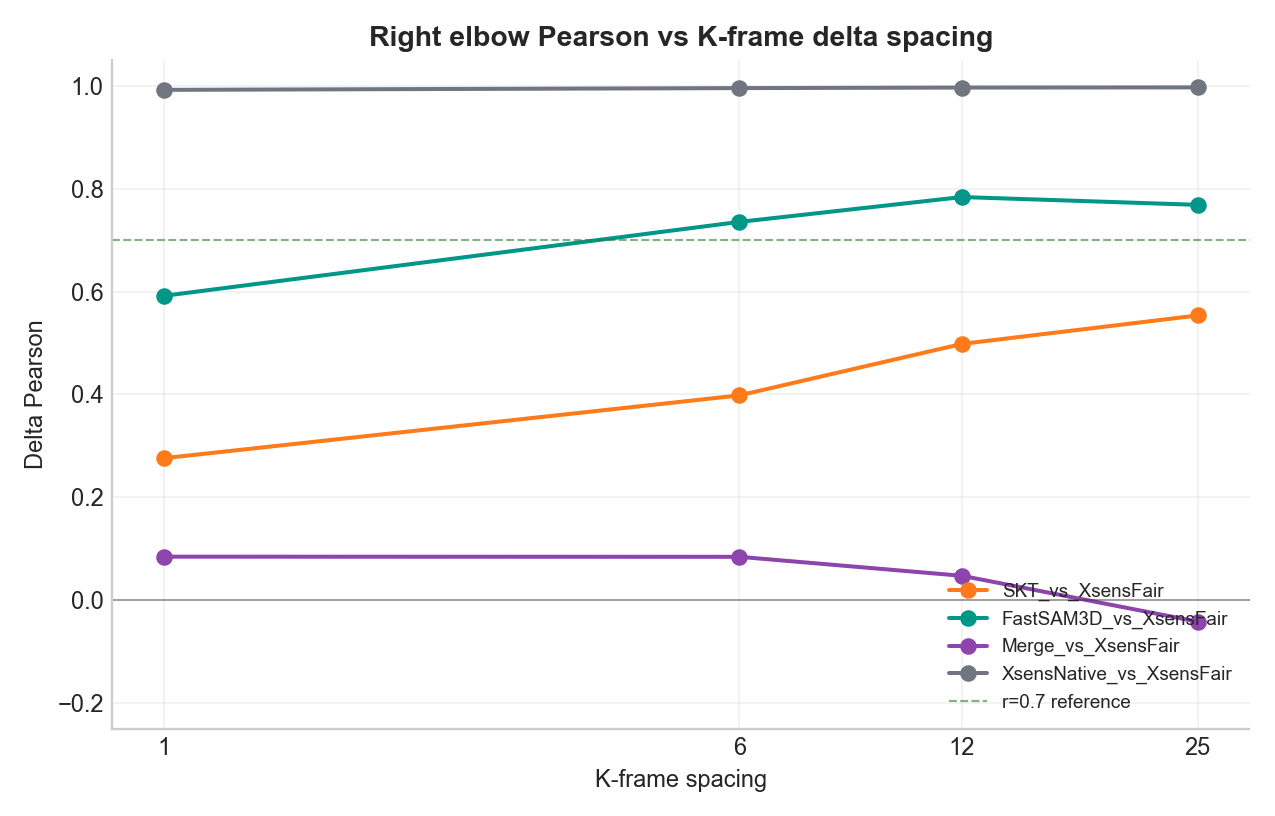
\includegraphics[width=\linewidth]{thesis_pearson_vs_k_rightelbow.png}
    \caption{Right elbow.}
  \end{subfigure}
  \caption{Motion-delta correlation as a function of K. The result supports using K=6 as a practical compromise between jitter sensitivity and motion interpretability.}
  \label{fig:pearson_vs_k}
\end{figure}

\subsection{Segment-level Results}

The segment-level track reinforces the frame-level motion finding while
adding two pieces of information that the frame-level numbers alone cannot
provide: per-segment range-of-motion (ROM) error in degrees, which is the
quantity most directly comparable to a ``movement size'' an ergonomist
would estimate manually, and per-segment normalised DTW distance, which
quantifies how similar the shape of motion through each segment is once
amplitude and offset are removed.
Aggregated over the detected active segments (39 for SKT, 45 for
FastSAM3D), FastSAM3D has both the lower mean ROM error (14.9\degr\ vs.\
26.9\degr\ for SKT) and the lower mean DTW distance (0.0355 vs.\ 0.0435).
The Xsens-native DTW distance ($\sim$6$\times 10^{-3}$) sets the lower
bound that the normalised DTW metric can reach on this dataset, so
FastSAM3D's $\sim$3.5$\times 10^{-2}$ is approximately six times the
reference floor, which is the right order of magnitude to claim
``competitive'' rather than ``saturated''.

\begin{table}[!htbp]
  \centering
  \caption{Segment-level summary over detected active movement intervals. Lower values are better.}
  \label{tab:segment_summary}
  \begin{tabular}{lccc}
    \toprule
    Method & Segments & Mean ROM error (\degr) $\downarrow$ & Mean DTW distance $\downarrow$ \\
    \midrule
    SKT & 39 & 26.9 & 0.0435 \\
    \good{FastSAM3D} & 45 & \good{14.9} & \good{0.0355} \\
    \textit{Xsens native check} & \textit{45} & \textit{4.8} & \textit{0.0062} \\
    \bottomrule
  \end{tabular}
\end{table}

\begin{figure}[!htbp]
  \centering
  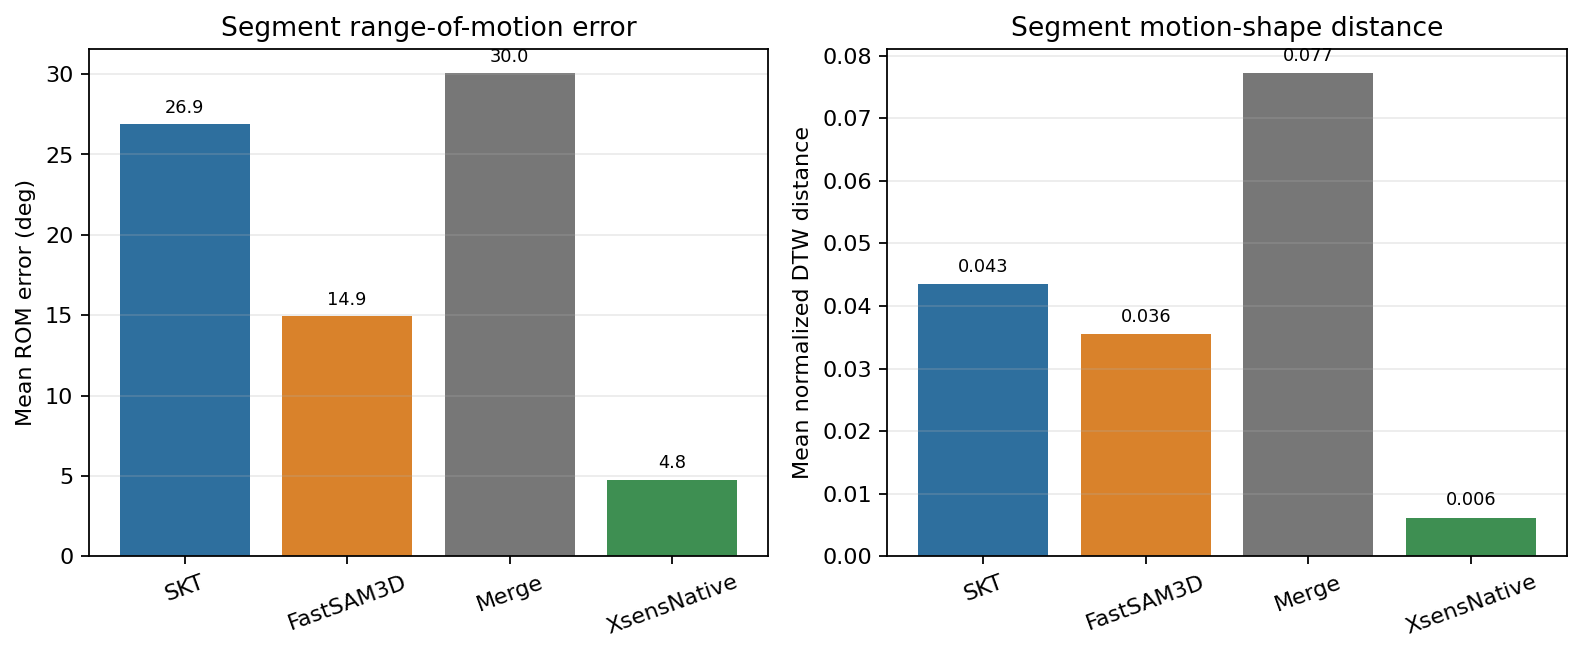
\includegraphics[width=0.95\linewidth]{thesis_segment_summary.png}
  \caption{Segment-level ROM error and DTW distance. FastSAM3D gives the strongest segment-level agreement among the vision methods, while the Xsens-native check provides a reference-system lower bound.}
  \label{fig:segment_summary_plot}
\end{figure}

\subsection{Position-space Results}

The position-space track produces a deliberately different interpretation
from the angle and motion tracks, and reading it as a competing
quality ranking would be a mistake.
SKT recovers 3D coordinates with metric scale inherited from calibrated
stereo geometry, so its distance to the Xsens-derived reference -- 30.6\,cm
mean (20.8\,cm median) after rigid Kabsch alignment -- is a meaningful
geometric quantity whose magnitude can be discussed in the same units as
the workspace itself.
FastSAM3D's direct distance to the Xsens reference under identical
coordinate assumptions is approximately 300\,cm, which is two orders of
magnitude larger; this number, however, does not say that FastSAM3D's
poses are visually two orders of magnitude worse -- it says that the raw
FastSAM3D output uses a different coordinate origin and scale convention,
and the dominant component of the 300\,cm distance is therefore a global
similarity transform that has not yet been resolved.
When FastSAM3D is instead aligned directly to SKT over a set of common
joints, the residual mean distance drops to approximately 60\,cm,
clarifying that the genuine inter-method 3D disagreement is at the
half-metre scale rather than the multi-metre scale and isolating it from
the coordinate-convention issue.

The methodological consequence is reported in
Table~\ref{tab:position_summary} rather than asserted in prose: the
position-space numbers must be read as \emph{coordinate/scale
diagnostics} that document the operational cost of using each method in
metric 3D space, not as another lap of the angle-space ranking
competition.
SKT inherits its metric scale automatically from the calibrated camera
baseline (Section~\ref{sec:data_setup}), so a downstream RULA scorer or
workspace-overlay tool can read its 3D coordinates directly; FastSAM3D
needs a separate scale/coordinate alignment step, which is feasible but
adds operational complexity that this thesis flags explicitly rather
than leaves implicit.

\begin{table}[!htbp]
  \centering
  \caption{Position-space diagnostic results. These values should be interpreted as coordinate/scale diagnostics rather than pure pose-quality rankings.}
  \label{tab:position_summary}
  \small
  \begin{tabularx}{\linewidth}{lccX}
    \toprule
    Comparison & Mean distance & Median distance & Notes \\
    \midrule
    SKT vs.\ reference & 30.6 cm & 20.8 cm & Metric stereo scale after rigid alignment \\
    FastSAM3D vs.\ reference & 300.3 cm & 294.8 cm & Coordinate/scale convention mismatch dominates \\
    FastSAM3D aligned to SKT & 60.0 cm & 36.3 cm & Direct inter-method skeleton comparison \\
    \bottomrule
  \end{tabularx}
\end{table}

\begin{figure}[!htbp]
  \centering
  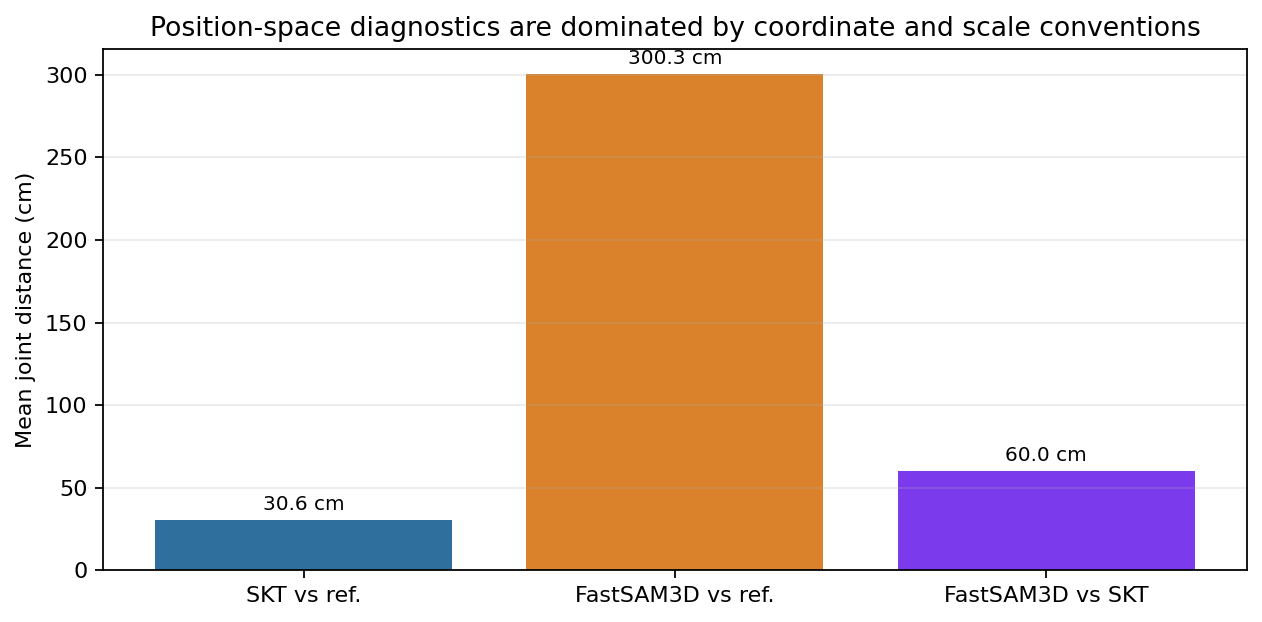
\includegraphics[width=0.9\linewidth]{thesis_position_diagnostic.png}
  \caption{Position-space diagnostic comparison. SKT is more meaningful in metric 3D space because it is tied to calibrated stereo geometry, whereas direct FastSAM3D-to-reference distance is dominated by coordinate and scale conventions.}
  \label{fig:position_diagnostic_plot}
\end{figure}

\subsection{Cross-method Synthesis}

Reading the two evaluation tracks together produces a more complete picture
than either gives on its own.
Table~\ref{tab:cross_method_synthesis} consolidates the headline numbers
for SKT and FastSAM3D (with the Xsens-native check shown alongside as a
reference-system floor).
FastSAM3D leads on the angle-space (lower MAE) and motion-space (higher
correlation) tracks, which together indicate that learned body and motion
priors suppress the per-frame jitter that hurts a frame-independent
sparse stereo reconstruction on this dataset.
SKT lags FastSAM3D on angle and motion but its 3D coordinates carry metric
scale by construction, and the per-frame geometric quality signals it exposes
(epipolar error, reprojection error, triangulation confidence) are exactly
the signals that downstream ergonomic quality gating requires.

\begin{table}[!htbp]
  \centering
  \caption{SKT vs FastSAM3D headline synthesis across evaluation tracks. Best value per column is highlighted; the Xsens-native row is a reference-system internal check, not a competing method.}
  \label{tab:cross_method_synthesis}
  \small
  \begin{tabular}{lccccl}
    \toprule
    Method & Angle MAE (\degr) $\downarrow$ & RULA bin agree.\ $\uparrow$ & Motion $r$ K=6 $\uparrow$ & Segment ROM (\degr) $\downarrow$ & Metric scale \\
    \midrule
    SKT
    & 17.6 & 0.540 & 0.379 & 26.9 & \good{Calibrated} \\
    \good{FastSAM3D}
    & \good{15.4} & \good{0.553} & \good{0.644} & \good{14.9} & Needs alignment \\
    \textit{Xsens native (ref.)}
    & \textit{4.7} & \textit{0.886} & \textit{0.965} & \textit{4.8} & \textit{---} \\
    \bottomrule
  \end{tabular}
\end{table}

The overall pattern is: \emph{the learning-based monocular pipeline wins
the angle and motion agreement tracks; the calibrated stereo pipeline
retains the deployment-geometry advantage; and neither replaces the other.}
This split is the substantive result of the synthesis and is what
Section~\ref{sec:discussion} examines in operational terms.

\clearpage
% =============================================================
\section{Discussion}
\label{sec:discussion}
% =============================================================

\subsection{Why FastSAM3D Performs Better in Angle and Motion Space}

The most likely reason FastSAM3D leads SKT on the angle and motion tracks
is that its learned body-structure and motion-continuity priors mask
exactly the per-frame failure mode that hurts a frame-independent
triangulation pipeline.
FastSAM3D's 3D output for any given frame is conditioned on body-shape
plausibility constraints that were absorbed from large pose-sequence
training corpora, so a momentarily unreliable keypoint produces a
smoothed-out anatomical correction rather than a sharp angle spike; this
is qualitatively visible in the K=6 elbow scatter plots
(Figure~\ref{fig:k6_elbow_scatter}), where the FastSAM3D scatter sits
along the ideal y=x diagonal whereas the SKT scatter shows recurring
vertical accumulation -- large target deltas at small reference deltas --
that no amount of point-density change can hide.
This shape of error matters for the interpretation: the SKT weakness is
not a uniform random noise floor but a structured failure pattern
concentrated on a small fraction of frames, which suggests that targeted
quality-aware repair rather than uniform smoothing is the appropriate
remedy.

\subsection{Why Stereo Geometry Still Matters}

The FastSAM3D advantage on the agreement tracks does not eliminate the
case for calibrated stereo geometry, because deployment in a real
manufacturing setting cares about two properties that the agreement
tracks alone do not test: whether the 3D coordinates are in real metric
units, and whether the system can flag its own unreliable frames before
they reach a downstream ergonomic risk score.
SKT inherits metric scale from the calibrated camera baseline, so its 3D
coordinates can be overlaid on workspace geometry without an additional
alignment step, whereas any monocular learning-based pipeline needs an
explicit external scale and coordinate recovery before its output is
usable in the same role.
More importantly, SKT exposes a per-frame geometric quality vector --
triangulation confidence, epipolar error, reprojection error,
left--right keypoint agreement -- whose individual components are tied
to the camera model, so an automated downstream stage can refuse to
score frames whose quality vector falls outside the working envelope;
an end-to-end learned pipeline can in principle be augmented with
calibrated uncertainty heads, but that augmentation is itself an open
research problem rather than a property the FastSAM3D output exposes
today.

\subsection{Failure-case Analysis of High-delta Events}

The K=6 scatter pattern noted above is not generic noise but a small
number of identifiable keypoint-chain failures, and treating it as
such is what makes the next SKT iteration tractable.
For elbow flexion, the relevant chain is shoulder--elbow--wrist; an
unstable wrist detection in either camera can leave the triangulated
shoulder and elbow correct, satisfy all geometric quality checks
individually, and still produce an elbow angle that jumps by tens of
degrees in a single frame, because the angle depends on the relative
direction of two segments rather than on the absolute position of any
single keypoint.
Figure~\ref{fig:skt_high_delta_cases} shows two representative SKT
high-delta intervals projected back onto the original video; the
problematic frames in each clip share three concrete characteristics --
partial occlusion of the wrist by the body or by an object, large
camera-to-subject distance, and inconsistent left/right detection of
the elbow chain -- rather than appearing at random across the
recording.
The operational implication is that the next SKT improvement should
focus on chain-aware (not single-keypoint-aware) quality filtering
together with short-window temporal repair, since both interventions
target the specific failure mode evidenced here and neither requires
changing the underlying triangulation or angle formula.

\subsection{Applicability Boundaries}

Putting these analyses together gives a concrete recommendation for
when each method type should be preferred in industrial ergonomic
monitoring, rather than a universal ranking statement.
For deployment scenarios that need only joint-angle outputs and short-term
motion signals -- for example a fixed-camera workstation that scores
postures from skeletons but does not need to overlay them on real
geometry -- a learning-based monocular pipeline of the FastSAM3D family
is the more competitive choice on this dataset, both because its
absolute angle MAE is lower and because its short-term motion signal is
visibly more stable.
For deployment scenarios that need metric 3D scale, workspace overlay,
or per-frame quality gating before downstream automated scoring -- which
is the more typical industrial setting -- calibrated stereo remains
the more defensible default, because both the metric coordinates and
the geometric quality signals are properties of the camera model rather
than of the trained model.
The thesis therefore does not recommend one method as universally
correct, and the practical question for any new deployment is which of
these two sets of requirements dominates.

\begin{figure}[!htbp]
  \centering
  \begin{subfigure}[b]{0.98\linewidth}
    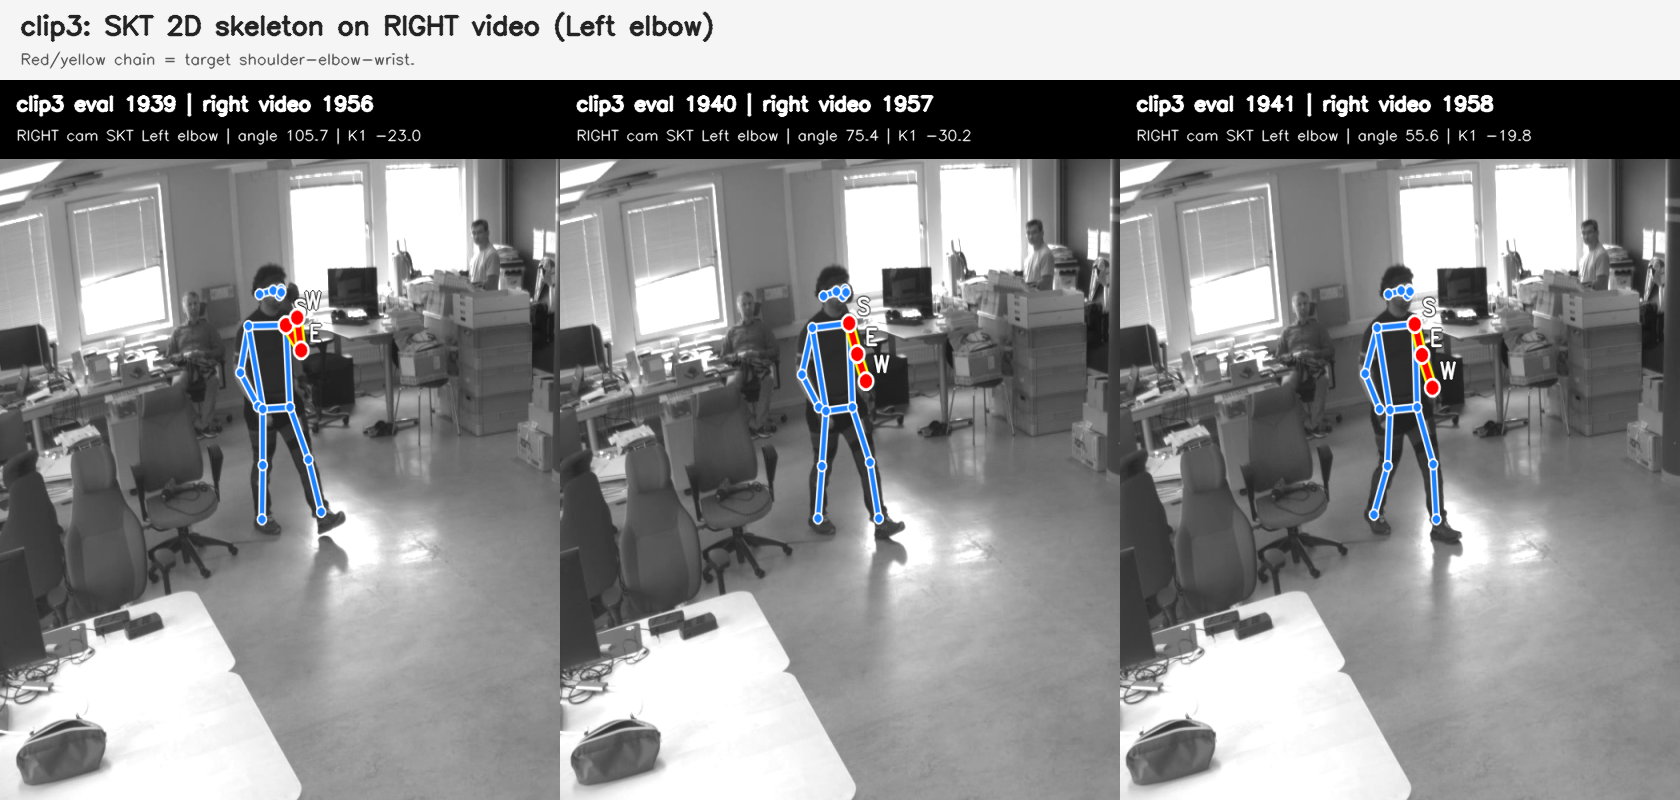
\includegraphics[width=\linewidth]{thesis_skt_high_delta_left_elbow_frames.png}
    \caption{Left-elbow high-delta interval.}
  \end{subfigure}

  \vspace{0.35cm}
  \begin{subfigure}[b]{0.98\linewidth}
    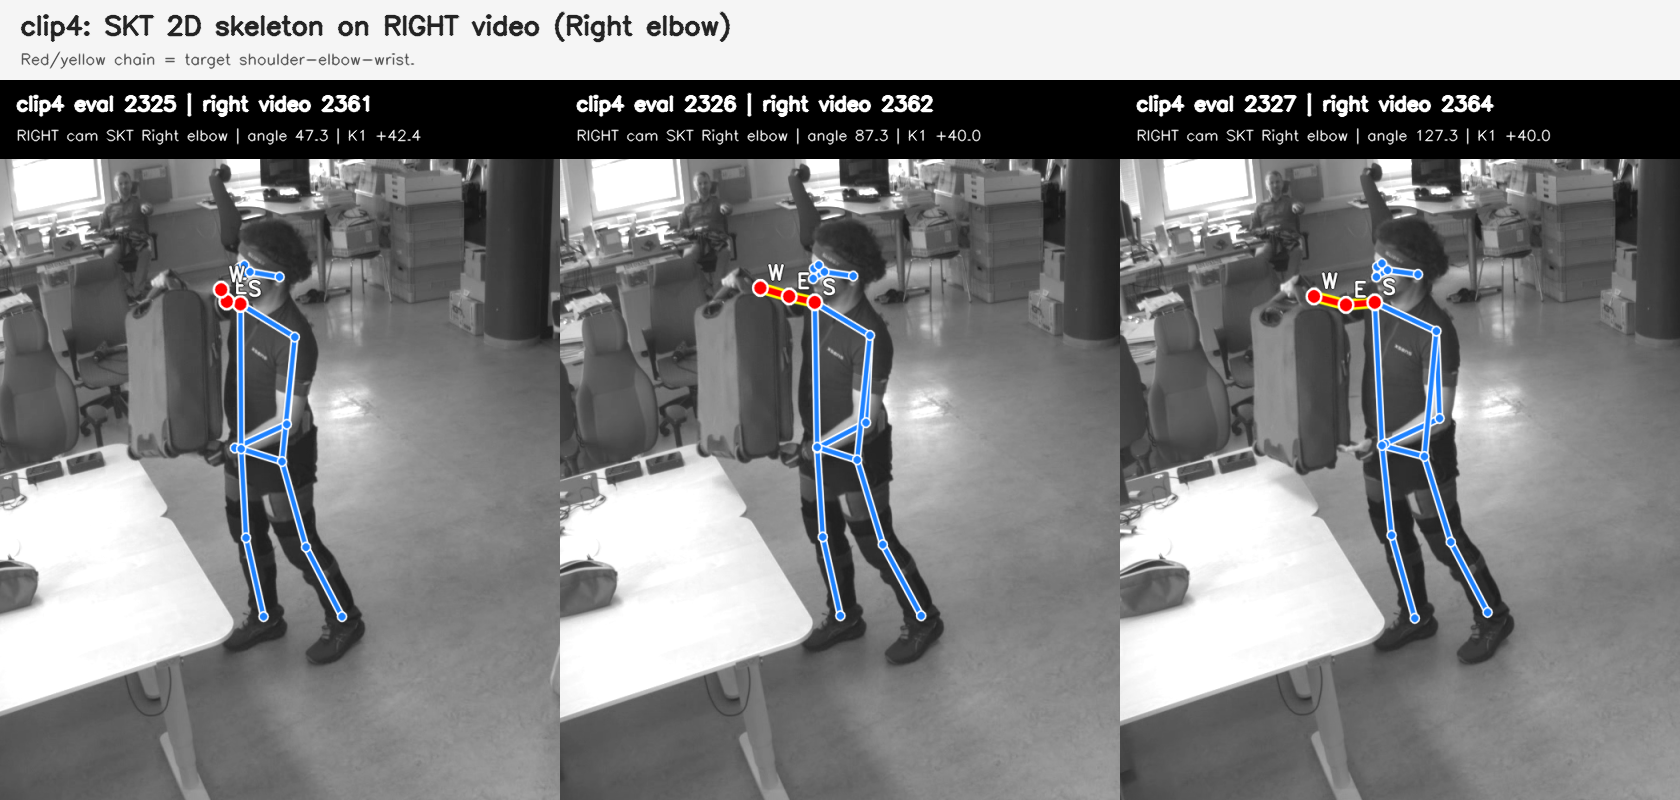
\includegraphics[width=\linewidth]{thesis_skt_high_delta_right_elbow_frames.png}
    \caption{Right-elbow high-delta interval.}
  \end{subfigure}
  \caption{Representative SKT high-delta diagnostic frames projected onto the original video view. These examples indicate that some large motion deltas are caused by local keypoint instability around the elbow chain rather than by physically implausible whole-body motion.}
  \label{fig:skt_high_delta_cases}
\end{figure}

\subsection{Limitations}

Four limitations of the present study set the boundary inside which all
quantitative results above should be read; they are stated explicitly here
so that the conclusion in Section~\ref{sec:conclusion} can rest on
honestly scoped evidence rather than on an over-generalised claim.
\emph{First}, all results come from a single subject performing a single
controlled recording in a manufacturing-like environment; the
between-method ranking should therefore be read as supported on this
dataset rather than as a general statement about every operator,
clothing style, lighting condition, or camera distance.
\emph{Second}, the deepest motion-space analysis focuses on the elbow,
which is the joint that the project investigated most carefully and the
joint whose Xsens calibration limitation is best quantified; the
motion-space numbers for the shoulder, hip, and knee are reported but
should be read with weaker confidence than the elbow numbers because
their reference floor is less well characterised.
\emph{Third}, the evaluation outputs depend on the smoothing window, the
segment-detection thresholds, and the constant-offset assumption used for
time alignment; the pipeline records these settings explicitly in the run
configuration so that any future work can rerun the same comparison under
different choices, and the synchronisation analysis in
Section~\ref{sec:data_setup} shows that the constant-offset assumption is
adequate for this recording but does not prove it for longer recordings.
\emph{Fourth}, Xsens is used throughout as an external comparison
reference and not as physical ground truth; the absolute angle errors are
therefore interpreted alongside the Xsens self-consistency floor
established in Section~\ref{sec:data_setup} rather than as direct error
against a true biomechanical zero.

\subsection{Implications for Real-time Deployment}

The deployment path that follows most cleanly from the above is to
prioritise getting the calibrated SKT pipeline running efficiently on
GPU hardware before treating learning-based pose models as
replacements rather than as optional stabilisers.
The concrete engineering steps are well-established: export the 2D pose
model to TensorRT, move video decoding and preprocessing onto the GPU,
and keep triangulation and joint-angle computation lightweight enough to
remain in the streaming budget; lightweight real-time pose models such
as RTMPose \cite{jiang2023rtmpose} make this direction realistic at the
2D-detection stage, although the final reportable number must be
end-to-end latency rather than model inference time alone, because
decoding, preprocessing, and post-processing each consume a measurable
share of the per-frame budget.
Once this baseline streams reliably, the two natural extensions are
(i) integrating a learning-based pose head -- of the FastSAM3D family --
as an optional smoothing or fallback signal when SKT quality flags drop
below an acceptable threshold, and (ii) introducing transformer-based
temporal priors to repair the keypoint-chain failures identified in the
high-delta analysis above; both extensions are framed here as
\emph{stabilisers on top of} the calibrated stereo baseline rather than
as replacements for it, because the deployment-geometry advantages
discussed in Section~7.2 do not transfer to a pure monocular pipeline
without additional scale/coordinate work.

\clearpage
% =============================================================
\section{Conclusion and Future Work}
\label{sec:conclusion}
% =============================================================

\subsection{Conclusion}

This thesis evaluates 3D human pose estimation for manufacturing-oriented
ergonomic monitoring using a three-axis framework -- angle-space,
motion-space, and position-space -- against an Xsens reference whose
calibration limitation is explicitly quantified rather than ignored.
On the single-subject manufacturing recording used here, the
learning-based monocular FastSAM3D pipeline delivers better
agreement-track numbers (mean angle MAE 15.4\degr\ vs.\ 17.6\degr; mean
K=6 motion Pearson 0.64 vs.\ 0.38; segment ROM error 14.9\degr\ vs.\
26.9\degr) than the calibrated stereo SKT pipeline.
SKT nevertheless retains the only metric-scale 3D output among the
evaluated pipelines and is the only pipeline that exposes per-frame
geometric quality signals usable for downstream quality gating, so it
remains the right choice when deployment requires real units or
self-reported reliability rather than only joint-angle smoothness.
The substantive conclusion is therefore not a single recommended method
but a deliberate split: learning-based monocular pose is competitive
when the deployment task is restricted to joint angles and short-term
motion, while calibrated stereo is necessary when the deployment task
extends to metric 3D scale and explainable per-frame quality, and a
future ergonomic monitoring system is likely to want both -- learned
priors for body-pose stability, stereo geometry for scale and
deployment transparency.

\subsection{Future Work}

Three follow-up directions are required before the present results can
be claimed as generally applicable rather than as evidence for a single
controlled recording.

\begin{enumerate}[leftmargin=1.2cm]
  \item \textbf{Validation on additional recordings and subjects.}
        Repeat the same three-axis protocol on at least one additional
        operator, additional clothing, additional lighting, and an
        unscripted task, in order to test whether the FastSAM3D
        agreement-track advantage generalises and whether the SKT
        high-delta failure modes recur in the same shoulder--elbow--wrist
        chain across subjects.
  \item \textbf{Real-time GPU deployment of SKT with optional learned
        stabilisers.} Move the SKT 2D backbone to TensorRT and the
        decoding/preprocessing onto the GPU, measure end-to-end streaming
        latency rather than model inference time alone, and then evaluate
        a FastSAM3D-style learned head as an optional smoothing or
        fallback signal triggered when SKT quality flags drop below the
        deployment threshold.
  \item \textbf{Beyond-elbow motion analysis and connection to a complete
        ergonomic risk score.} Extend the motion-space analysis to the
        shoulder, hip, and knee with the same reference-floor
        quantification that this thesis applies to the elbow, and then
        connect the resulting joint-angle stream to a full ergonomic
        risk score (e.g.\ RULA, REBA) rather than to RULA-bin agreement
        alone, so that pose-estimation quality and downstream
        risk-classification quality can be reported as a single
        deployment-relevant pipeline.
\end{enumerate}

\subsection{Recommended Next-stage Experimental Protocol}

To make the validation-on-new-datasets step above repeatable rather than
ad hoc, this subsection consolidates the working protocol used in the
present recording into a five-stage checklist
(Table~\ref{tab:validation_checklist}) that future datasets should run
\emph{in order}, with each stage gating the next.
The protocol enforces two methodological principles that emerged from
the present study.
The first principle is that data-ingestion integrity (orientation,
frame-ID re-pairing, timestamp monotonicity, calibration compatibility)
must be verified before any accuracy number is computed, because the
most expensive class of failure in the present pipeline is
mis-interpreting an ingestion bug as a pose-estimation result.
The second principle is that algorithmic changes and protocol changes
must be evaluated separately: if SKT is later modified with stronger
2D-keypoint filtering or a temporal repair module, the same K-frame
motion-delta protocol must be rerun before and after the modification
so that the comparison is fair, and if a new learning-based method is
added, its coordinate convention and filtering state must be recorded
before it is included in the position-space analysis.

\begin{table}[!htbp]
  \centering
  \caption{Five-stage validation checklist for extending the present thesis evaluation to new manufacturing recordings. Stages should be executed in order; each stage gates the next.}
  \label{tab:validation_checklist}
  \small
  \begin{tabularx}{\linewidth}{p{3.2cm}XX}
    \toprule
    Stage & What should be checked & Why it matters \\
    \midrule
    Dataset validation
    & Video orientation, hardware frame IDs, metadata timestamps, synchronised frame count, and camera calibration compatibility.
    & Prevents data-ingestion errors from being mis-interpreted as pose-estimation errors. \\
    Time alignment
    & Automatic offset curves on three independent scores, residual lag at the beginning and end of the recording, and common valid intervals.
    & Ensures that motion-space metrics compare the same physical movement period. \\
    Method comparison
    & Angle MAE, K-frame motion agreement at $K\in\{1,6,12,25\}$, segment ROM and DTW, and position-space diagnostics for every method.
    & Keeps the comparison multi-dimensional and avoids over-ranking methods by a single metric. \\
    Failure analysis
    & High-delta frames, occlusion cases, camera distance, and left--right keypoint consistency.
    & Connects quantitative outliers to concrete visual causes and guides targeted SKT repair work. \\
    Deployment check
    & End-to-end streaming latency, GPU preprocessing, model inference time, and stability under streaming input.
    & Tests whether the method can move from offline evaluation toward real-time ergonomic monitoring. \\
    \bottomrule
  \end{tabularx}
\end{table}

The final thesis version should therefore deliver two distinct kinds of
evidence rather than a single aggregate error number.
The first is \emph{quantitative agreement} across several recordings and
movement types, run through the checklist above so that the comparison
remains multi-dimensional and protocol-controlled.
The second is \emph{diagnostic evidence} that exposes when and why each
pipeline fails and which subsystem is responsible, of the kind that
Section~\ref{sec:discussion} presented for the SKT high-delta cases.
This combination is the right level of evidence for ergonomic deployment
in manufacturing, because a practical monitoring system needs not only
to be accurate on average but also to know -- and to expose -- when its
output should not be trusted.

\clearpage
% =============================================================
\appendix
\clearpage
% =============================================================

\section{Stereo Calibration Parameters}
\label{app:calibration}

The numerical calibration values reported below are the optimised parameters
that all SKT experiments in the thesis use as fixed input; the
binary form is stored at \texttt{shared/camera\_params.npz} and is loaded
directly by the pose pipeline.
The intrinsic matrices follow the OpenCV convention $K = [[f_x, 0, c_x];
[0, f_y, c_y]; [0,0,1]]$ in pixels, the distortion vectors follow the
14-parameter rational model used by OpenCV's \texttt{cv2.calibrateCamera}
(only the first 8 entries are non-zero in this calibration), and the
stereo extrinsics give the rotation $R$ and translation $T$ that map a
3D point from the left to the right camera frame in centimetres.

\begin{table}[!htbp]
  \centering
  \caption{Left and right camera intrinsic matrices (pixels) and the stereo extrinsic baseline.}
  \label{tab:calib_intrinsics}
  \small
  \begin{tabular}{lcc}
    \toprule
    Quantity & Left camera & Right camera \\
    \midrule
    $f_x$ (pixels)            & 1130.27 & 1129.01 \\
    $f_y$ (pixels)            & 1130.35 & 1129.63 \\
    $c_x$ (pixels)            & 1019.32 & 1028.31 \\
    $c_y$ (pixels)            &  825.72 &  826.35 \\
    \midrule
    Stereo baseline $\|T\|$   & \multicolumn{2}{c}{41.27\,cm} \\
    Image resolution          & \multicolumn{2}{c}{2048 $\times$ 1536} \\
    Distortion model          & \multicolumn{2}{c}{OpenCV rational (14-parameter)} \\
    \bottomrule
  \end{tabular}
\end{table}

The stereo rotation $R$ deviates from the identity by less than 0.011
radians on each off-diagonal entry, consistent with a near-aligned
parallel-baseline rig, and the translation vector
$T \approx [-41.27, -0.03, 0.04]^T$\,cm confirms that the baseline is
dominated by the $x$ axis as designed.
The essential matrix $E$ and fundamental matrix $F$ recorded in
\texttt{camera\_params.npz} are derived from $R$ and $T$ together with
the two intrinsic matrices and are not duplicated here.
The full distortion coefficients and the original calibration session
metadata (target type, number of valid views, per-view reprojection
residuals) are stored alongside the matrices in the same NPZ file.

\FloatBarrier
\clearpage
\section{Sensitivity Analyses}
\label{app:sensitivity}

The headline numbers reported in Section~\ref{sec:results} depend on
three parameter choices made in the evaluation pipeline: the camera-side
smoothing window, the activity-segment detection threshold, and the
DTW preprocessing convention.
This appendix reports how the SKT motion and segment-level numbers move
when each choice is varied, so that the reader can judge how brittle the
conclusion is.

\begin{table}[!htbp]
  \centering
  \caption{Sensitivity of SKT motion-space and segment-level numbers to the camera-side moving-average smoothing window, on the present recording. The 200\,ms and 300\,ms rows are identical because both round to a 3-frame centred window at 12.5\,fps.}
  \label{tab:sens_smoothing}
  \footnotesize
  \setlength{\tabcolsep}{4pt}
  \resizebox{\linewidth}{!}{%
  \begin{tabular}{lcccc}
    \toprule
    Window & Frames & SKT K=6 Pearson (L/R) & SKT ROM MAE (L/R, \degr) & K=1 quiet std (L/R, \degr) \\
    \midrule
    100\,ms & 1 & -- / --   & 38.4 / 33.3 & --   / --   \\
    200\,ms & 3 & 0.41 / 0.40 & 19.3 / 21.3 & 7.0 / 6.6 \\
    300\,ms & 3 & 0.41 / 0.40 & 19.3 / 21.3 & 7.0 / 6.6 \\
    400\,ms & 5 & 0.43 / 0.42 & 16.4 / 21.8 & 4.4 / 4.5 \\
    \bottomrule
  \end{tabular}%
  }
\end{table}

The 200\,ms working point chosen in the main body is the
literature-supported rule of thumb for non-explosive human motion; a
400\,ms window further reduces SKT quiet-frame jitter below the
$<$5\degr/frame validation target at the cost of a slightly weaker
short-term motion signal, and is reported here as the
``conservative-smoothing'' alternative for future runs.

\begin{table}[!htbp]
  \centering
  \caption{Sensitivity of detected segment counts to the activity-detection threshold (applied to the Xsens-derived reference K-frame deltas).}
  \label{tab:sens_segments}
  \small
  \begin{tabular}{lcc}
    \toprule
    Activity threshold (\degr) & Left-elbow segments & Right-elbow segments \\
    \midrule
    8  & 5  & 7  \\
    10 (default) & 8 & 9 \\
    12 & 13 & 15 \\
    \bottomrule
  \end{tabular}
\end{table}

Segment counts vary by a factor of roughly 2--3 across the tested
threshold range, but the cross-method ranking inside each row is stable:
FastSAM3D maintains the lowest segment ROM MAE and DTW distance
regardless of the threshold setting, so the main-body conclusion does
not depend on the specific threshold value chosen.
The DTW preprocessing sweep (\texttt{mean\_l2}, \texttt{mean}, and
\texttt{none}) confirms that the mean-subtracted, L2-normalised
convention adopted in the main body is the version under which the
XsensNative-vs-XsensFair anchor DTW remains near zero; without L2
normalisation the DTW distance becomes dominated by amplitude rather
than by shape, which is the explicit motivation for the chosen
preprocessing.

\FloatBarrier
\clearpage
\section{Implementation and Reproducibility Notes}
\label{app:repro}

The standalone evaluation workflow is implemented in
\texttt{00\_pose\_pipeline/}.
For the present dataset, the main reproduction command is:
\begin{footnotesize}
\begin{verbatim}
/opt/anaconda3/envs/pose/bin/python \
  00_pose_pipeline/src/run_pipeline.py \
  --config \
  00_pose_pipeline/configs/current_2025_ergonomics.yaml \
  --stages \
  validate,offset,angle,motion,segment,scatter
\end{verbatim}
\end{footnotesize}

The configuration file records the dataset-specific choices that
otherwise must be inferred from prose alone: the 180\degr\ video
rotation, the hardware-frame-ID synchronisation rule, the metadata
timestamp-parsing convention, the calibration NPZ path, the per-system
smoothing settings, the K-frame list $\{1,6,12,25\}$, the
activity-detection threshold, and the automatic offset-search range.
Generated outputs are stored under \texttt{00\_pose\_pipeline/runs/}
and include both the headline tables/figures referenced from the main
body and the per-stage diagnostics that drive Section~\ref{sec:discussion}.

Figure~\ref{fig:residual_lag_check} reports a residual lag diagnostic
that the pipeline can produce after the selected constant offset has
been applied; it is not a headline result but it documents the
sanity-check evidence used to defend the constant-offset assumption in
Section~\ref{sec:data_setup}.

\begin{figure}[!htbp]
  \centering
  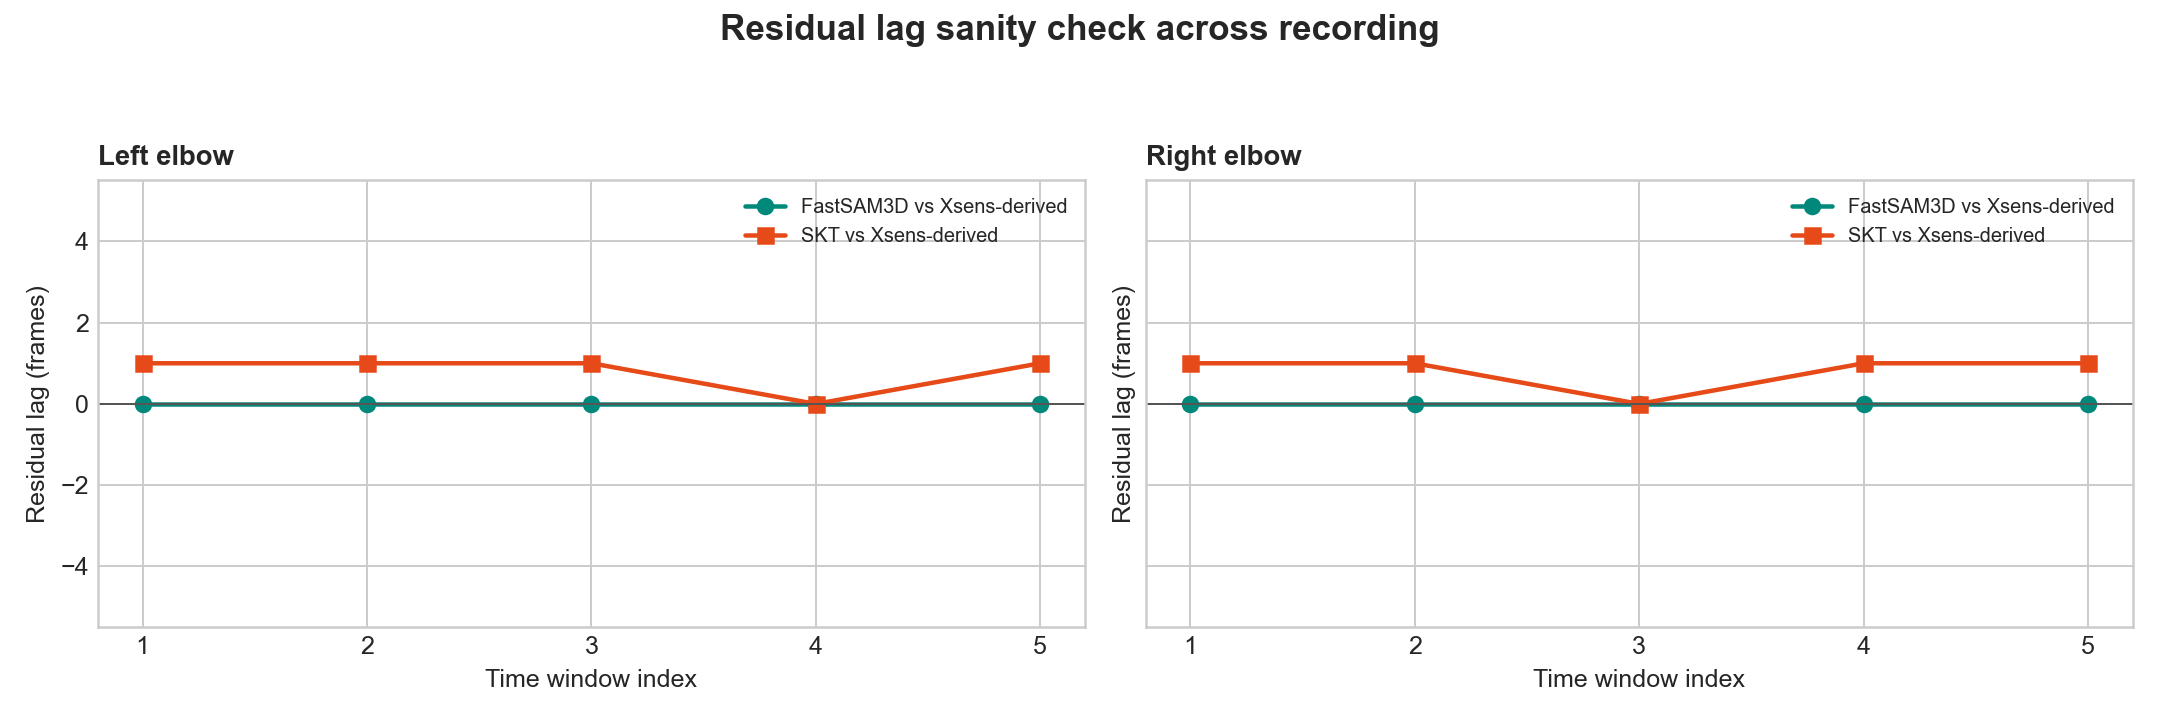
\includegraphics[width=\linewidth]{thesis_residual_lag_drift_check.png}
  \caption{Residual lag sanity check after applying the selected constant offset. The figure supports the assumption that a constant offset is adequate for the present recording, while explicitly acknowledging that future longer or multi-take recordings should rerun this check.}
  \label{fig:residual_lag_check}
\end{figure}

\FloatBarrier
\clearpage
\section{Claim-evidence Self-review}
\label{app:claim_evidence}

The table below maps every major thesis claim back to its supporting
evidence in this draft, following the
``Claim $|$ Evidence $|$ Status'' convention recommended for
adversarial paper review.
Claims marked \emph{Needs evidence} are stated as open items rather
than as supported conclusions, and the conclusion in
Section~\ref{sec:conclusion} is restricted to the claims marked
\emph{Supported}.

\begin{table}[H]
  \centering
  \caption{Claim-evidence map for the present thesis draft.}
  \label{tab:claim_evidence}
  \small
  \renewcommand{\arraystretch}{1.12}
  \begin{tabularx}{\linewidth}{p{4.0cm}Xp{1.9cm}}
    \toprule
    Claim & Evidence used in this draft & Status \\
    \midrule
    FastSAM3D is stronger than SKT in angle-space on the present dataset.
    & Table~\ref{tab:angle_summary} and Figure~\ref{fig:angle_summary_plot}: 15.4\degr\ mean MAE vs.\ 17.6\degr.
    & Supported \\
    FastSAM3D is stronger than SKT in K=6 motion-space agreement.
    & Table~\ref{tab:motion_summary}, Figure~\ref{fig:motion_k6_summary_plot}, and Figure~\ref{fig:k6_elbow_scatter}: mean Pearson 0.644 vs.\ 0.379; elbow correlations 0.54/0.69 vs.\ 0.39/0.39.
    & Supported \\
    SKT retains a position-space and interpretability advantage.
    & Table~\ref{tab:position_summary}, Figure~\ref{fig:position_diagnostic_plot}, and the SKT method design; SKT uses calibrated stereo scale and exposes per-frame geometric quality signals.
    & Supported \\
    A constant cross-system offset is adequate for the current recording.
    & Figure~\ref{fig:offset_search}, Figure~\ref{fig:first_last_delta}, and Figure~\ref{fig:residual_lag_check}; the three independent offset scores converge within $\sim$0.04\,s.
    & Supported for present recording \\
    SKT high-delta points are caused by local keypoint-chain instability.
    & Figure~\ref{fig:skt_high_delta_cases}: diagnostic frames show partial wrist occlusion, large camera distance, and inconsistent left/right elbow-chain detection during the high-delta intervals.
    & Supported qualitatively \\
    The SKT vs FastSAM3D ranking is robust to smoothing and segmentation parameters.
    & Appendix~\ref{app:sensitivity}: sensitivity tables across smoothing windows and activity thresholds preserve the FastSAM3D $>$ SKT ranking.
    & Supported \\
    Results generalise to manufacturing environments broadly.
    & Only one controlled single-subject dataset is evaluated.
    & Needs evidence \\
    Full RULA automation is solved.
    & Only continuous angle MAE and RULA-like bin agreement are reported; RULA scoring requires additional load/twist/repetition information.
    & Not claimed \\
    \bottomrule
  \end{tabularx}
\end{table}

\clearpage

\begin{thebibliography}{99}

\bibitem{mcatamney1993rula}
L.~McAtamney and E.~N.~Corlett,
\textit{RULA: a survey method for the investigation of work-related upper limb disorders},
Applied Ergonomics, vol.~24, no.~2, pp.~91--99, 1993.

\bibitem{menolotto2020motion}
M.~Menolotto, D.-S.~Komaris, S.~Tedesco, B.~O'Flynn, and M.~Walsh,
\textit{Motion capture technology in industrial applications: A systematic review},
Sensors, vol.~20, no.~19, article 5687, 2020.

\bibitem{yu2019joint}
Y.~Yu, X.~Yang, H.~Li, X.~Luo, and H.~Guo,
\textit{Joint-level vision-based ergonomic assessment tool for construction workers},
Journal of Construction Engineering and Management, vol.~145, no.~5, 2019.

\bibitem{menanno2024ergonomic}
M.~Menanno, C.~Riccio, V.~Benedetto, and G.~Palmieri,
\textit{An ergonomic risk assessment system based on 3D human pose estimation and collaborative robot},
Applied Sciences, vol.~14, no.~11, article 4823, 2024.

\bibitem{quesada2026supporting}
A.~Quesada Diaz, A.~Iriondo Pascual, L.~Hanson, D.~H{\"o}gberg, and A.~Syberfeldt,
\textit{Supporting ergonomics evaluations in manufacturing: A comparison of computer vision- and IMU-based motion capture},
IOP Conference Series: Materials Science and Engineering, vol.~1342, article 012053, 2026.

\bibitem{iriondo2024development}
A.~Iriondo Pascual, L.~Hanson, D.~H{\"o}gberg, E.~Brolin, and A.~Syberfeldt,
\textit{Development and initial usability evaluation of a digital tool for simulation-based multi-objective optimization of productivity and worker well-being},
Advanced Engineering Informatics, vol.~60, article 102726, 2024.

\bibitem{iriondo2025integrating}
A.~Iriondo Pascual, L.~Hanson, E.~Brolin, D.~H{\"o}gberg, and A.~Syberfeldt,
\textit{Integrating motion capture and digital human modelling tools for worker ergonomics assessment: A case study from experimental lab to real-world manufacturing},
Lecture Notes in Computer Science, vol.~15828, pp.~324--333, 2025.

\bibitem{filippeschi2017survey}
A.~Filippeschi, N.~Schmitz, M.~Miezal, G.~Bleser, E.~Ruffaldi, and D.~Stricker,
\textit{Survey of motion tracking methods based on inertial sensors: A focus on upper limb human motion},
Sensors, vol.~17, no.~6, article 1257, 2017.

\bibitem{roetenberg2009xsens}
D.~Roetenberg, H.~Luinge, and P.~Slycke,
\textit{Xsens MVN: Full 6DOF human motion tracking using miniature inertial sensors},
Xsens Technologies technical report, 2009.

\bibitem{cao2019openpose}
Z.~Cao, G.~Hidalgo, T.~Simon, S.-E.~Wei, and Y.~Sheikh,
\textit{OpenPose: Realtime multi-person 2D pose estimation using part affinity fields},
IEEE Transactions on Pattern Analysis and Machine Intelligence,
vol.~43, no.~1, pp.~172--186, 2019.

\bibitem{jiang2023rtmpose}
T.~Jiang, P.~Lu, L.~Zhang, N.~Ma, R.~Han, C.~Lyu, Y.~Li, and K.~Chen,
\textit{RTMPose: Real-time multi-person pose estimation based on MMPose},
arXiv preprint arXiv:2303.07399, 2023.

\bibitem{pavllo20193d}
D.~Pavllo, C.~Feichtenhofer, D.~Grangier, and M.~Auli,
\textit{3D human pose estimation in video with temporal convolutions and semi-supervised training},
Proceedings of the IEEE/CVF Conference on Computer Vision and Pattern Recognition, pp.~7753--7762, 2019.

\bibitem{zhu2023motionbert}
W.~Zhu, X.~Ma, Z.~Liu, L.~Liu, W.~Wu, and Y.~Wang,
\textit{MotionBERT: A unified perspective on learning human motion representation},
Proceedings of the IEEE/CVF International Conference on Computer Vision, pp.~15085--15099, 2023.

\bibitem{yang2026fastsam3d}
T.~Yang, S.~He, H.~Jing, J.~Yang, Z.~Liu, C.~Zou, and Y.~Wang,
\textit{Fast SAM 3D Body: Accelerating SAM 3D Body for Real-Time Full-Body Human Mesh Recovery},
arXiv preprint arXiv:2603.15603, 2026.

\bibitem{hartley2004multiple}
R.~Hartley and A.~Zisserman,
\textit{Multiple View Geometry in Computer Vision},
2nd ed., Cambridge University Press, 2004.

\bibitem{hirschmuller2007sgbm}
H.~Hirschm{\"u}ller,
\textit{Stereo processing by semiglobal matching and mutual information},
IEEE Transactions on Pattern Analysis and Machine Intelligence,
vol.~30, no.~2, pp.~328--341, 2007.

\bibitem{kabsch1976solution}
W.~Kabsch,
\textit{A solution for the best rotation to relate two sets of vectors},
Acta Crystallographica, Section A, vol.~32, pp.~922--923, 1976.

\bibitem{sakoe1978dtw}
H.~Sakoe and S.~Chiba,
\textit{Dynamic programming algorithm optimization for spoken word recognition},
IEEE Transactions on Acoustics, Speech, and Signal Processing,
vol.~26, no.~1, pp.~43--49, 1978.

\bibitem{perezluque2026reaching}
E.~P{\'e}rez Luque, S.~Lee, D.~H{\"o}gberg, J.~Yang, and M.~Lamb,
\textit{Predicting human upper extremity reaching motions: Comparison of optimization-based method and heuristic method},
International Journal of Human--Computer Interaction, 2026.
DOI: 10.1080/10447318.2026.2632154.

\end{thebibliography}

\end{document}

% =============================================================

\documentclass[12pt,a4paper]{article}

\usepackage[margin=2.5cm]{geometry}
\usepackage{fontspec}
\defaultfontfeatures{Ligatures=TeX}
\usepackage{amsmath,amssymb}
\usepackage{siunitx}
\usepackage{booktabs}
\usepackage{graphicx}
\usepackage{subcaption}
\usepackage[table]{xcolor}
\usepackage{hyperref}
\usepackage{microtype}
\usepackage{parskip}
\usepackage{enumitem}
\usepackage{array}
\usepackage{float}
\usepackage{tabularx}
\usepackage{setspace}
\usepackage{placeins}
\usepackage{caption}

\hypersetup{colorlinks=true, linkcolor=blue!70!black, urlcolor=blue!70!black, citecolor=green!50!black}
\graphicspath{{figures/}}
\emergencystretch=2em
\setstretch{1.06}
\setlength{\textfloatsep}{1.1em plus 0.25em minus 0.2em}
\setlength{\floatsep}{1.0em plus 0.25em minus 0.2em}
\setlength{\intextsep}{1.0em plus 0.25em minus 0.2em}
\captionsetup{font=small, labelfont=bf}

\definecolor{goodcolor}{rgb}{0.00,0.38,0.18}
\definecolor{warncolor}{rgb}{0.55,0.27,0.07}
\definecolor{badcolor}{rgb}{0.65,0.10,0.10}
\newcommand{\good}[1]{\textcolor{goodcolor}{\textbf{#1}}}
\newcommand{\warn}[1]{\textcolor{warncolor}{\textbf{#1}}}
\newcommand{\bad}[1]{\textcolor{badcolor}{\textbf{#1}}}
\newcommand{\degr}{\ensuremath{^\circ}}

\title{\textbf{Posture and Activity Detection in Manufacturing Environments\\Using 3D Vision and AI}}
\author{Fanbo Meng\\
\small Chalmers University of Technology\\
\small In collaboration with Viscando AB}
\date{Master's Thesis Draft, June 2026}

\begin{document}
\maketitle
\tableofcontents
\newpage

% =============================================================
\section*{Abstract}
% =============================================================

Ergonomic risk assessment in manufacturing demands pose-estimation systems
that are spatially accurate, temporally consistent, and interpretable at the
joint-angle level, yet the dominant evaluation practice in the pose-estimation
literature still relies on a single distance metric such as Mean Per-Joint
Position Error, which is not sufficient to decide whether a method is fit for
ergonomic monitoring.
This thesis revisits 3D human pose estimation for manufacturing settings by
comparing a calibrated stereo keypoint triangulation pipeline (SKT) with a
monocular learning-based pipeline (FastSAM3D); an Xsens inertial motion-capture
suit is used as an external reference system rather than as absolute ground
truth, because its body-model calibration introduces systematic angle offsets
that must be acknowledged in the evaluation design.
The evaluation is organized around three complementary axes -- angle-space
accuracy, motion-space consistency, and position-space geometry -- and the
motion-space axis is built on K-frame angle deltas
($\Delta_K\theta_t = \theta_t-\theta_{t-K}$), which cancel the static Xsens
offset by differencing and expose true short-term motion agreement.
On a single-subject manufacturing recording of 2801 synchronized stereo frame
pairs over 248.8\,s, FastSAM3D achieves lower mean angle MAE than SKT across
eight body angles (15.4\degr\ vs.\ 17.6\degr) and stronger K=6 motion-delta
correlation with the Xsens-derived reference (mean Pearson 0.64 vs.\ 0.38;
right-elbow Pearson 0.69 vs.\ 0.39).
This angle and motion advantage is attributed to FastSAM3D's learned
body-shape and motion-continuity priors, which absorb anatomical constraints
from large training corpora and consequently suppress the per-frame keypoint
jitter that a frame-independent geometric triangulation pipeline propagates
directly into its angle estimates.
SKT, by contrast, retains a clear position-space advantage: its 3D coordinates
inherit metric scale directly from the calibrated stereo baseline without any
external alignment step, and the per-frame geometric quality signals it
exposes~-- epipolar error, reprojection error, triangulation confidence~--
provide deployment-ready reliability indicators that a monocular learning-based
pipeline does not offer natively.
These findings indicate that the two approaches are complementary rather than
interchangeable: learned monocular pose estimation is the more competitive
choice when angle accuracy and temporal motion smoothness are the primary
requirements, while calibrated stereo triangulation remains essential when
metric 3D coordinates and transparent per-frame reliability are needed for
downstream ergonomic quality control.

% =============================================================
\newpage
\section{Introduction}
% =============================================================

\subsection{Motivation}

Work-related musculoskeletal disorders remain one of the dominant
occupational-health burdens in manufacturing, and the established
countermeasure is repeated ergonomic risk assessment of operators while they
perform actual production tasks.
The standard observational instruments for such assessment, including the
Rapid Upper Limb Assessment (RULA), depend on a trained observer who manually
classifies joint postures into discrete risk categories
\cite{mcatamney1993rula}; this practice is labour-intensive, observer
dependent, and impossible to deploy at the temporal resolution that modern
just-in-time production demands.
Camera-based 3D human pose estimation offers a path toward continuous,
non-intrusive ergonomic monitoring, because the joint angles needed for RULA
and similar instruments can in principle be read directly from a body
skeleton reconstructed from video.

Realising this promise on the factory floor changes what counts as ``good''
pose estimation.
The dominant benchmarks in the pose-estimation literature reward
visually-plausible skeletons and low Mean Per-Joint Position Error (MPJPE) on
short, well-lit, frontal-view clips; an ergonomic monitoring system, however,
must produce joint-angle estimates that are temporally stable across long
shifts, robust to occlusion and dark workwear, and traceable to interpretable
quality signals when downstream automated risk scoring is involved.
This thesis therefore treats pose estimation as a measurement problem that
sits between multi-view geometry, learning-based vision, and application-level
ergonomic evaluation, and it organises its evaluation around the properties
that ergonomic deployment actually requires rather than around a single
geometric distance metric.

\subsection{Problem Statement and Scope}

The thesis investigates 3D body-keypoint and joint-angle estimation from a
calibrated stereo camera setup in a manufacturing-like environment, with the
deployment target being downstream ergonomic risk monitoring rather than
generic motion reconstruction.
The primary pose-estimation method developed in the thesis is Sparse
Keypoint Triangulation (SKT), in which a 2D pose detector is run on
synchronised left and right video streams and the matched keypoints are
triangulated into 3D under the calibrated stereo geometry; the study then
benchmarks SKT against a monocular learning-based pipeline (FastSAM3D).

A central methodological constraint is that no laboratory-grade optical
motion-capture system was available for the full manufacturing recording, so
this thesis adopts an Xsens inertial suit as an \emph{external reference
system}, deliberately avoiding the language of ``absolute ground truth''.
This wording is not cosmetic: the Xsens body model is calibrated through a
short on-subject procedure that can absorb true global orientation and
introduce a systematic per-joint offset, most visibly at the elbow.
Reporting only absolute joint-angle MAE against such a reference therefore
risks transferring the reference's calibration bias into a verdict about the
vision pipeline, and the evaluation design must counter this by reporting
relative-change metrics (frame-to-frame K-frame angle deltas) in parallel
with absolute angles, since differencing cancels any static offset that the
two systems may carry.

\subsection{Research Questions}

The thesis is structured around three research questions:

\begin{enumerate}[label=\textbf{RQ\arabic*:}, leftmargin=1.8cm]
  \item How accurately can a calibrated stereo keypoint triangulation
        pipeline (SKT) recover the eight ergonomically relevant upper- and
        lower-body joint angles in a manufacturing-style recording, when
        absolute and motion-space accuracy are reported in parallel against
        an Xsens-derived reference?
  \item Under a unified evaluation protocol (shared timeline, common
        smoothing policy, identical reference), how does the geometry-based
        SKT pipeline compare with the learning-based FastSAM3D pipeline in
        (i) absolute angle accuracy and (ii) K-frame motion consistency at
        $K\in\{1,6,12,25\}$ frames?
  \item Which pipeline properties beyond raw accuracy -- in particular
        per-frame quality signals, metric scale, and resilience to
        occlusion and low-texture industrial backgrounds -- decide whether
        a method is fit for real-time ergonomic monitoring on GPU hardware?
\end{enumerate}

\subsection{Contributions}

In addressing the three research questions, the thesis makes the following
contributions:

\begin{itemize}[leftmargin=1.2cm]
  \item \textbf{A reproducible stereo pose pipeline (SKT)} that combines
        synchronised 2D keypoint detection, calibrated DLT triangulation,
        three-point geometric joint-angle computation, and per-frame
        geometry-aware quality signals (triangulation confidence, epipolar
        error, reprojection error) that can drive downstream quality gating.
  \item \textbf{A three-axis evaluation framework} -- angle-space, motion-space,
        position-space -- that exposes method-property tradeoffs which a single
        MPJPE-style metric would conceal, and that is reusable across other
        vision pipelines on the same dataset.
  \item \textbf{An explicit cross-system synchronisation and filtering protocol},
        including automatic temporal-offset estimation against three independent
        scores, hardware-frame-ID re-pairing for non-monotonic stereo
        timestamps, and a per-system smoothing policy (no extra smoothing on
        the already heavily filtered Xsens reference, unified 200\,ms moving
        average on the camera-based methods).
  \item \textbf{An empirical comparison} that finds the monocular learning-based
        FastSAM3D pipeline more competitive than the calibrated stereo SKT on
        both angle MAE and K-frame motion correlation for this manufacturing
        recording, while showing that SKT retains an irreplaceable advantage
        in metric 3D scale and in geometry-aware quality control needed for
        deployment.
\end{itemize}

\subsection{Thesis Structure}

The remainder of the thesis is organised as follows.
Section~\ref{sec:background} reviews relevant work on 3D human pose
estimation, vision-based ergonomic assessment, and reference-system
limitations.
Section~\ref{sec:data_setup} describes the stereo capture system, the
2025 ergonomics dataset, the Xsens reference data, and the cross-system
time-synchronisation procedure.
Section~\ref{sec:methods} presents the two evaluated pose-estimation
pipelines (SKT and FastSAM3D).
Section~\ref{sec:evaluation} defines the three-axis evaluation framework and
the unified filtering policy.
Section~\ref{sec:results} reports the angle-space, motion-space,
segment-level, and position-space results, and synthesises them across
methods.
Section~\ref{sec:discussion} discusses applicability boundaries, failure
modes, and limitations, and
Section~\ref{sec:conclusion} concludes and outlines future work.

\clearpage
% =============================================================
\section{Background and Related Work}
\label{sec:background}
% =============================================================

\subsection{3D Human Pose Estimation}

3D human pose estimation recovers either explicit body keypoints or
parametric body-model parameters from one or several camera streams, and the
existing literature divides clearly along whether the recovery uses one view
or multiple views.
Monocular approaches estimate 3D pose from a single image or video, either
through a two-stage 2D--detection + 3D--lifting pipeline or through an
end-to-end regression that maps image features directly to 3D coordinates.
Real-time 2D pose estimators such as OpenPose and RTMPose have established
that the 2D detection stage can be made fast and accurate enough for online
use \cite{cao2019openpose,jiang2023rtmpose}, and temporal 3D models such as
VideoPose3D and MotionBERT have shown that body-motion priors can be learned
from large pose-sequence corpora and used to stabilise the lifting step
\cite{pavllo20193d,zhu2023motionbert}.
The structural limitation of any monocular pipeline, however, is that the
absolute distance from camera to subject is not directly observed; depth and
metric scale must be inferred from learned body proportions or recovered
through an external alignment step, which is acceptable for visual
animation but problematic for ergonomic measurement.

Stereo and multi-view approaches replace this scale ambiguity with explicit
multi-view geometry.
In a calibrated two-camera setup, an epipolar relation constrains where a
point seen in the left view must appear in the right view, and the intersection
of the two corresponding viewing rays gives a 3D coordinate that inherits its
scale directly from the measured baseline; this geometric chain, together with
the intrinsic and extrinsic camera matrices recovered during calibration,
forms the standard machinery of multi-view computer vision
\cite{hartley2004multiple}.
Stereo pipelines also split into a sparse and a dense branch: sparse
triangulation matches a small number of 2D keypoints across views and
triangulates each one independently, which is fast and interpretable but
sensitive to per-keypoint jitter and to left--right mismatches, whereas
dense disparity methods such as Semi-Global Block Matching estimate depth at
every pixel \cite{hirschmuller2007sgbm} and then read off the joint depths,
which gives a denser geometric description but degrades sharply on the
low-texture clothing and visually ambiguous backgrounds that are common in
real industrial scenes.

\subsection{Pose Evaluation Methodology}

Pose-estimation errors do not project equally onto every evaluation space,
and reporting only one metric can hide the property that actually matters
for the downstream application.
\emph{Position-space} evaluation, dominated in the literature by Mean
Per-Joint Position Error (MPJPE), measures the 3D Euclidean distance between
estimated and reference joints after rigid alignment, and it is the natural
metric when the goal is reconstruction geometry.
\emph{Angle-space} evaluation instead asks whether the joint angles computed
from the estimated skeleton are quantitatively correct, which is the
question that ergonomic risk instruments such as RULA actually answer
\cite{mcatamney1993rula}; a method can have low MPJPE while still placing
an elbow flexion in a different RULA risk bin, and the reverse is also
possible.
\emph{Motion-space} evaluation looks at the temporal change of pose, for
example through frame-to-frame angle deltas, and is the most useful axis when
the reference system itself carries a static calibration offset, because
differencing cancels that offset and isolates true motion agreement.
This thesis therefore reports all three axes and treats no single metric as
sufficient on its own.

The ergonomic side of the evaluation is anchored by RULA, a screening
instrument that maps upper-limb and body postures to discrete risk
categories based on joint-angle ranges \cite{mcatamney1993rula}.
Because RULA depends primarily on angles rather than on absolute 3D
positions, the thesis treats RULA-like bin agreement as an
\emph{application-level classification metric} for selected joints alongside
the continuous angle MAE; it deliberately does not claim to implement a
complete automated RULA scoring system, since full RULA also requires
external information about loads, twisting, and repetition that the vision
pipeline alone cannot infer.
This narrower scope keeps the comparison focused on the pose-estimation
component while still connecting it to the deployment intent.

Vision-based ergonomic assessment has been studied increasingly in recent
years, and systematic reviews note that motion-capture technologies are
becoming common in industrial workplaces but that deployment quality still
depends on usability, measurement reliability, and task-specific
interpretation \cite{menolotto2020motion}.
Concrete vision-based ergonomic systems have been proposed in
construction \cite{yu2019joint} and in collaborative-robot settings
\cite{menanno2024ergonomic}, and the most directly relevant comparison study
to this thesis is the work of Quesada Diaz, Iriondo Pascual, and co-authors,
who explicitly compared computer-vision and IMU-based motion capture for
manufacturing ergonomics and highlighted the same recurrent themes of
careful filtering, cross-system alignment, and reference-aware benchmarking
that this thesis adopts \cite{quesada2026supporting}.
Iriondo Pascual's broader work on simulation-based productivity and
worker-wellbeing optimisation further situates the present thesis within
human-centred manufacturing and digital ergonomics
\cite{iriondo2024development,iriondo2025integrating}.

\subsection{Reference Systems}

The evaluation of any vision pose pipeline ultimately depends on what counts
as the reference, and inertial motion-capture systems such as Xsens have
become the practical default outside the optical-mocap laboratory because
they record high-frequency full-body motion without external cameras or
markers \cite{roetenberg2009xsens,filippeschi2017survey}.
The same convenience, however, is the source of the systematic limitation
that motivates the evaluation design of this thesis: the Xsens body-model
calibration is performed through a short on-subject N-pose / T-pose
procedure that absorbs the true global orientation and resets each segment
into the system's internal reference frame, and the resulting per-joint
angles can therefore carry an unknown static offset relative to a true
biomechanical zero, an effect that is particularly visible at the elbow.
For this reason the thesis consistently treats Xsens as an
\emph{external comparison / reference system} rather than as absolute
ground truth, and reserves the language of physical ground truth for
higher-grade systems such as optical mocap or per-joint goniometry that are
outside the scope of the present recording.

Within the Xsens output itself the thesis distinguishes between
\emph{Xsens native} joint angles, which are read directly from the MVNX
joint-angle channel and follow the Xsens body model and its internal
conventions, and \emph{Xsens-derived geometric} angles, which are
re-computed from the Xsens 3D segment positions using the same three-point
formula that is later applied to all vision pipelines.
The Xsens-derived geometric representation is adopted as the main reference
throughout the thesis because it removes the angle-definition mismatch
between systems, and because its agreement with the native representation
(MAE $\approx$ 2\degr\ in motion-space on the present recording) supplies a
quantitative lower-bound that calibrates how to interpret the absolute
errors reported for the vision methods.

\subsection{Related Work Summary and Positioning}

The closest prior work compares an IMU suit with a single vision pipeline
on industrial-style tasks \cite{quesada2026supporting} and concludes that
vision is promising but that filtering and alignment must be reported
carefully; the present thesis extends this line in three concrete ways.
First, it benchmarks two independently produced vision pipelines
side-by-side on the same recording -- a calibrated sparse-stereo pipeline
(SKT) and a monocular learning-based pipeline (FastSAM3D) -- so that the
geometry-versus-learning tradeoff is quantified rather than asserted.
Second, it replaces the single-metric evaluation that dominates the
pose-estimation literature with an explicit three-axis framework
(angle / motion / position), and it makes the motion axis robust to
reference-system calibration offsets by reporting K-frame angle deltas at
multiple time scales.
Third, it treats reference-system limitations as a first-class methodological
concern: the thesis quantifies the Xsens self-consistency floor on the same
metrics that are applied to the vision pipelines, so that every reported
number can be read against the lower bound of what the reference itself can
support.
The contribution is therefore not a new pose-estimation algorithm but a
deployment-oriented evaluation protocol, together with the empirical finding
that on this dataset learning-based monocular pose is competitive on angle
and motion while calibrated stereo retains an irreplaceable role in metric
scale and geometry-aware quality control.

\clearpage
% =============================================================
\section{Data and Experimental Setup}
\label{sec:data_setup}
% =============================================================

\subsection{Stereo Capture System}

All recordings used in this thesis come from a synchronised two-camera
stereo rig operated by Viscando AB.
Each camera captures at 2048$\times$1536 pixels and a nominal frame rate of
12.5\,fps, and the two streams are time-tagged at acquisition with a
hardware frame identifier together with a microsecond-resolution metadata
timestamp; the hardware identifier is what makes a robust left--right pairing
possible later, because the metadata timestamps alone can drift on either
side.
Because the cameras are physically mounted upside-down in the production
fixture, every frame is rotated by 180\degr\ before pose estimation is run,
so that gravity-up matches the assumption of the downstream pose detector
and skeleton orientation.

\subsection{Camera Calibration}

The geometric chain that maps a pair of 2D keypoints into a 3D coordinate
relies on accurate camera calibration, and small calibration errors are
amplified twice -- first when the rays are triangulated and again when three
3D points are turned into an angle -- so calibration quality is treated here
as a first-class methodological input rather than as a routine setup step.
The current calibration was estimated from an asymmetric circular-dot
target under a rational distortion model and yields a stereo baseline of
41.27\,cm with sub-pixel reprojection residuals on the calibration images;
the full intrinsic, distortion, and extrinsic matrices are reported in
Appendix~A and are treated as fixed inputs for all SKT
experiments in this thesis.

Figure~\ref{fig:calibration_evolution} documents the calibration refinement
that led to the current parameters and shows why the refinement was
necessary.
The first calibration attempt produced a geometrically consistent stereo
pair but estimated a baseline that was visibly off the measured physical
baseline of the rig, together with a reprojection error above the
working threshold that downstream triangulation can tolerate; the refined
and finally optimised calibration moved the estimated baseline back onto
the physical value and pushed the reprojection error into the sub-pixel
range, which is the regime in which the SKT pipeline produces stable
angle estimates rather than amplified jitter.

\begin{figure}[!htbp]
  \centering
  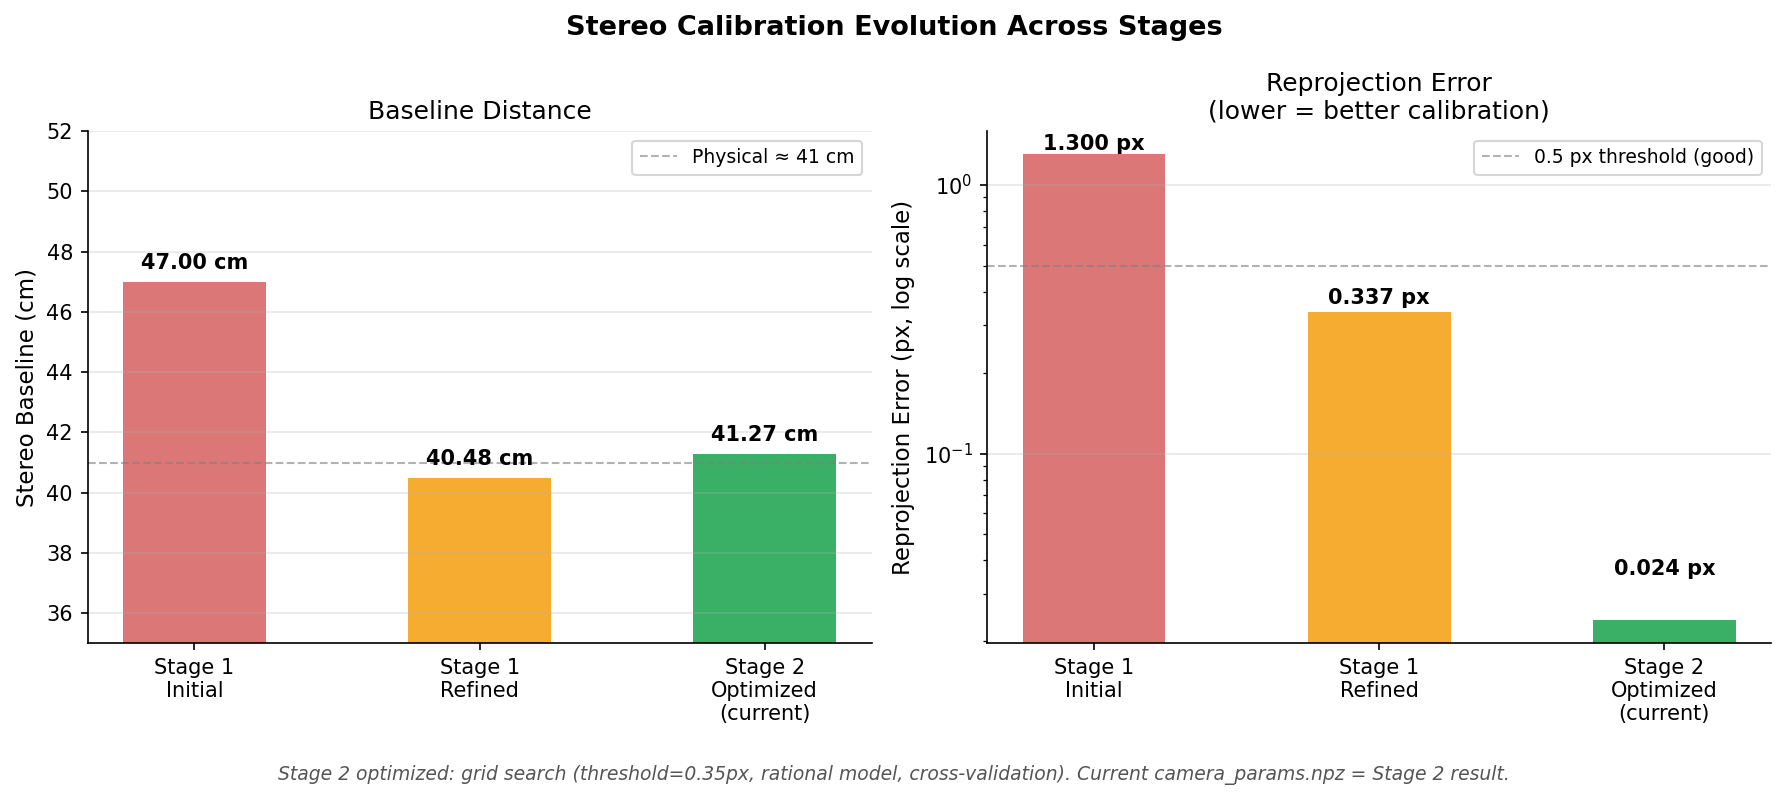
\includegraphics[width=\linewidth]{calibration_evolution.png}
  \caption{Stereo calibration evolution. The current calibration balances a realistic baseline estimate with a low reprojection error, making it suitable as the fixed geometric input for SKT.}
  \label{fig:calibration_evolution}
\end{figure}

\subsection{2025 Ergonomics Dataset}

All quantitative results in this thesis are computed on a single
single-subject ergonomics recording collected in a controlled
manufacturing-like environment, and this is therefore the dominant
generalisability limitation of the present study.
The subject performs a representative mix of factory-floor activities --
walking, sitting, squatting, reaching, lifting, and interacting with
furniture -- so that all major upper- and lower-body postures are exercised
within a single contiguous take rather than as isolated short clips.
After left--right pairing by hardware frame identifier, the usable
synchronised camera timeline contains 2801 frame pairs spanning 248.8\,s,
which corresponds to an effective frame rate of 12.5\,fps; the left raw
metadata contains 3015 rows and the right raw metadata contains 2882 rows,
so a non-trivial fraction of each side is either unpaired or falls outside
the synchronised interval, which is exactly what motivates the explicit
hardware-ID re-pairing step rather than reliance on raw row indices.
Table~\ref{tab:timeline_summary} summarises the resulting working timeline
that all downstream evaluations share.

\begin{table}[!htbp]
  \centering
  \caption{Summary of the synchronized camera timeline used for evaluation.}
  \label{tab:timeline_summary}
  \begin{tabular}{lc}
    \toprule
    Quantity & Value \\
    \midrule
    Synchronized frame pairs & 2801 \\
    Duration & 248.8 s \\
    Median frame interval & 0.0800 s \\
    Effective frame rate & 12.50 fps \\
    Left metadata rows & 3015 \\
    Right metadata rows & 2882 \\
    Rotation applied & 180\degr \\
    \bottomrule
  \end{tabular}
\end{table}

\subsection{Xsens Reference Data and Angle Representations}

The Xsens recording supplies full-body motion data on an independent time
axis and contains two distinct angle representations that the thesis must
choose between before any cross-method comparison can be reported.
The first is the \emph{Xsens native} joint-angle output, which is read
directly from the MVNX joint-angle channels and follows the Xsens body
model together with its internal axis and zero conventions.
The second is the \emph{Xsens-derived geometric} angle representation, in
which the joint angles are re-computed from the Xsens 3D segment positions
using the same three-point arccosine formula that is later applied to the
vision pipelines; this representation is adopted as the main reference
throughout the thesis because it removes the angle-definition mismatch
between the reference and the vision methods at the cost of being a
slightly less direct read of the Xsens body model.

The comparison between the two Xsens representations is then re-used as a
quantitative reference-system sanity check rather than discarded.
At the elbow, the two representations agree to within approximately
1--1.5\degr\ MAE in absolute angle space, and they agree to a Pearson
correlation of $\sim$0.99 in K-frame motion space; at the shoulder and hip,
the agreement is visibly weaker because the underlying axis conventions
differ more.
The implication for the thesis evaluation design is two-fold.
First, the elbow numbers serve as a \emph{lower-bound anchor}: a vision
method whose absolute angle MAE against Xsens-derived geometric is several
times the elbow self-consistency floor is unlikely to be limited by the
reference, whereas one that approaches the floor is approaching the
information limit of the reference itself.
Second, the larger shoulder/hip mismatch is one of the reasons the thesis
reports motion-space metrics alongside absolute angle MAE, since
differencing cancels both the unknown global Xsens calibration offset and
much of the axis-definition mismatch between the two representations.

\subsection{Cross-system Time Synchronisation}

Cross-system synchronisation is unavoidable for the present setup because
the cameras and the Xsens suit run on independent clocks, and any
mis-alignment converts directly into degraded motion-space agreement, so
the thesis adopts an automatic three-score offset search rather than a
manually picked shift.
The procedure first sweeps the offset coarsely between 0 and 30\,s, then
refines around the best candidate; at every candidate it computes three
independent agreement scores -- a position-space score on the 3D segment
positions, an angle-space score on the joint angles, and a motion-delta
score on the K-frame angle deltas -- and selects the motion-delta optimum
as the final offset because the motion evaluation is the most sensitive of
the three to residual sub-second mis-alignment.

For the present recording, the selected offset is 17.31\,s, and the
position-, angle-, and motion-delta optima fall at 17.27\,s, 17.28\,s, and
17.31\,s respectively.
The fact that three scores derived from three independent error spaces
converge inside a window of about 0.04\,s is the strongest evidence
available in this thesis that a single constant offset is an adequate
alignment model for this recording: had the underlying clock relation been
non-constant, the three scores would not be expected to peak so close
together.
Figure~\ref{fig:offset_search} shows the score curves produced by the
search and visualises this triple agreement.

\begin{figure}[!htbp]
  \centering
  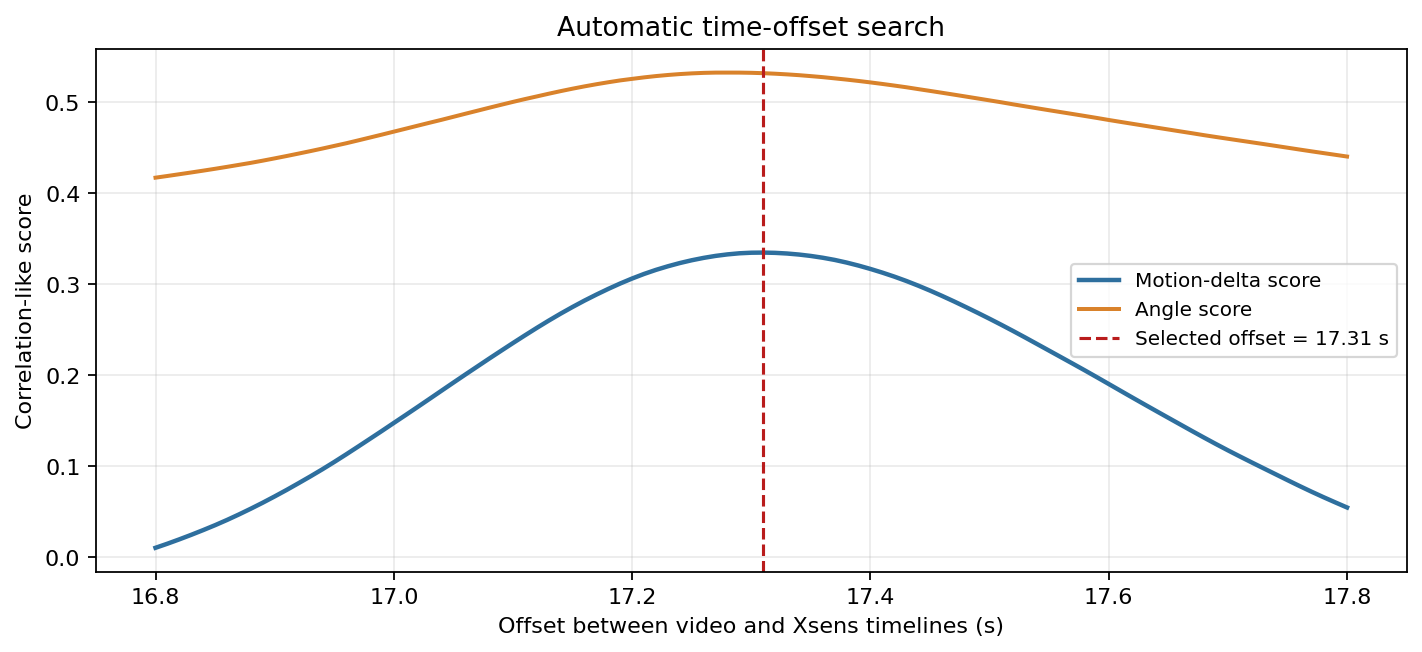
\includegraphics[width=\linewidth]{thesis_offset_search.png}
  \caption{Automatic offset estimation between the camera timeline and the Xsens reference timeline. The final selected value is 17.31 s, with position-, angle-, and motion-based scores all supporting a similar alignment.}
  \label{fig:offset_search}
\end{figure}

A second, qualitative synchronisation check is provided by overlaying the
aligned elbow-angle curves from all systems on the shared timeline
(Figure~\ref{fig:angle_time_alignment}).
The purpose of this plot is not to rank methods at the angle level -- that
is the task of Section~\ref{sec:results} -- but to confirm that the main
movement phases of the recording line up across systems after the offset
has been applied, so that any residual short-term deviation can be
attributed to true method behaviour rather than to an unfixed global shift.

\begin{figure}[!htbp]
  \centering
  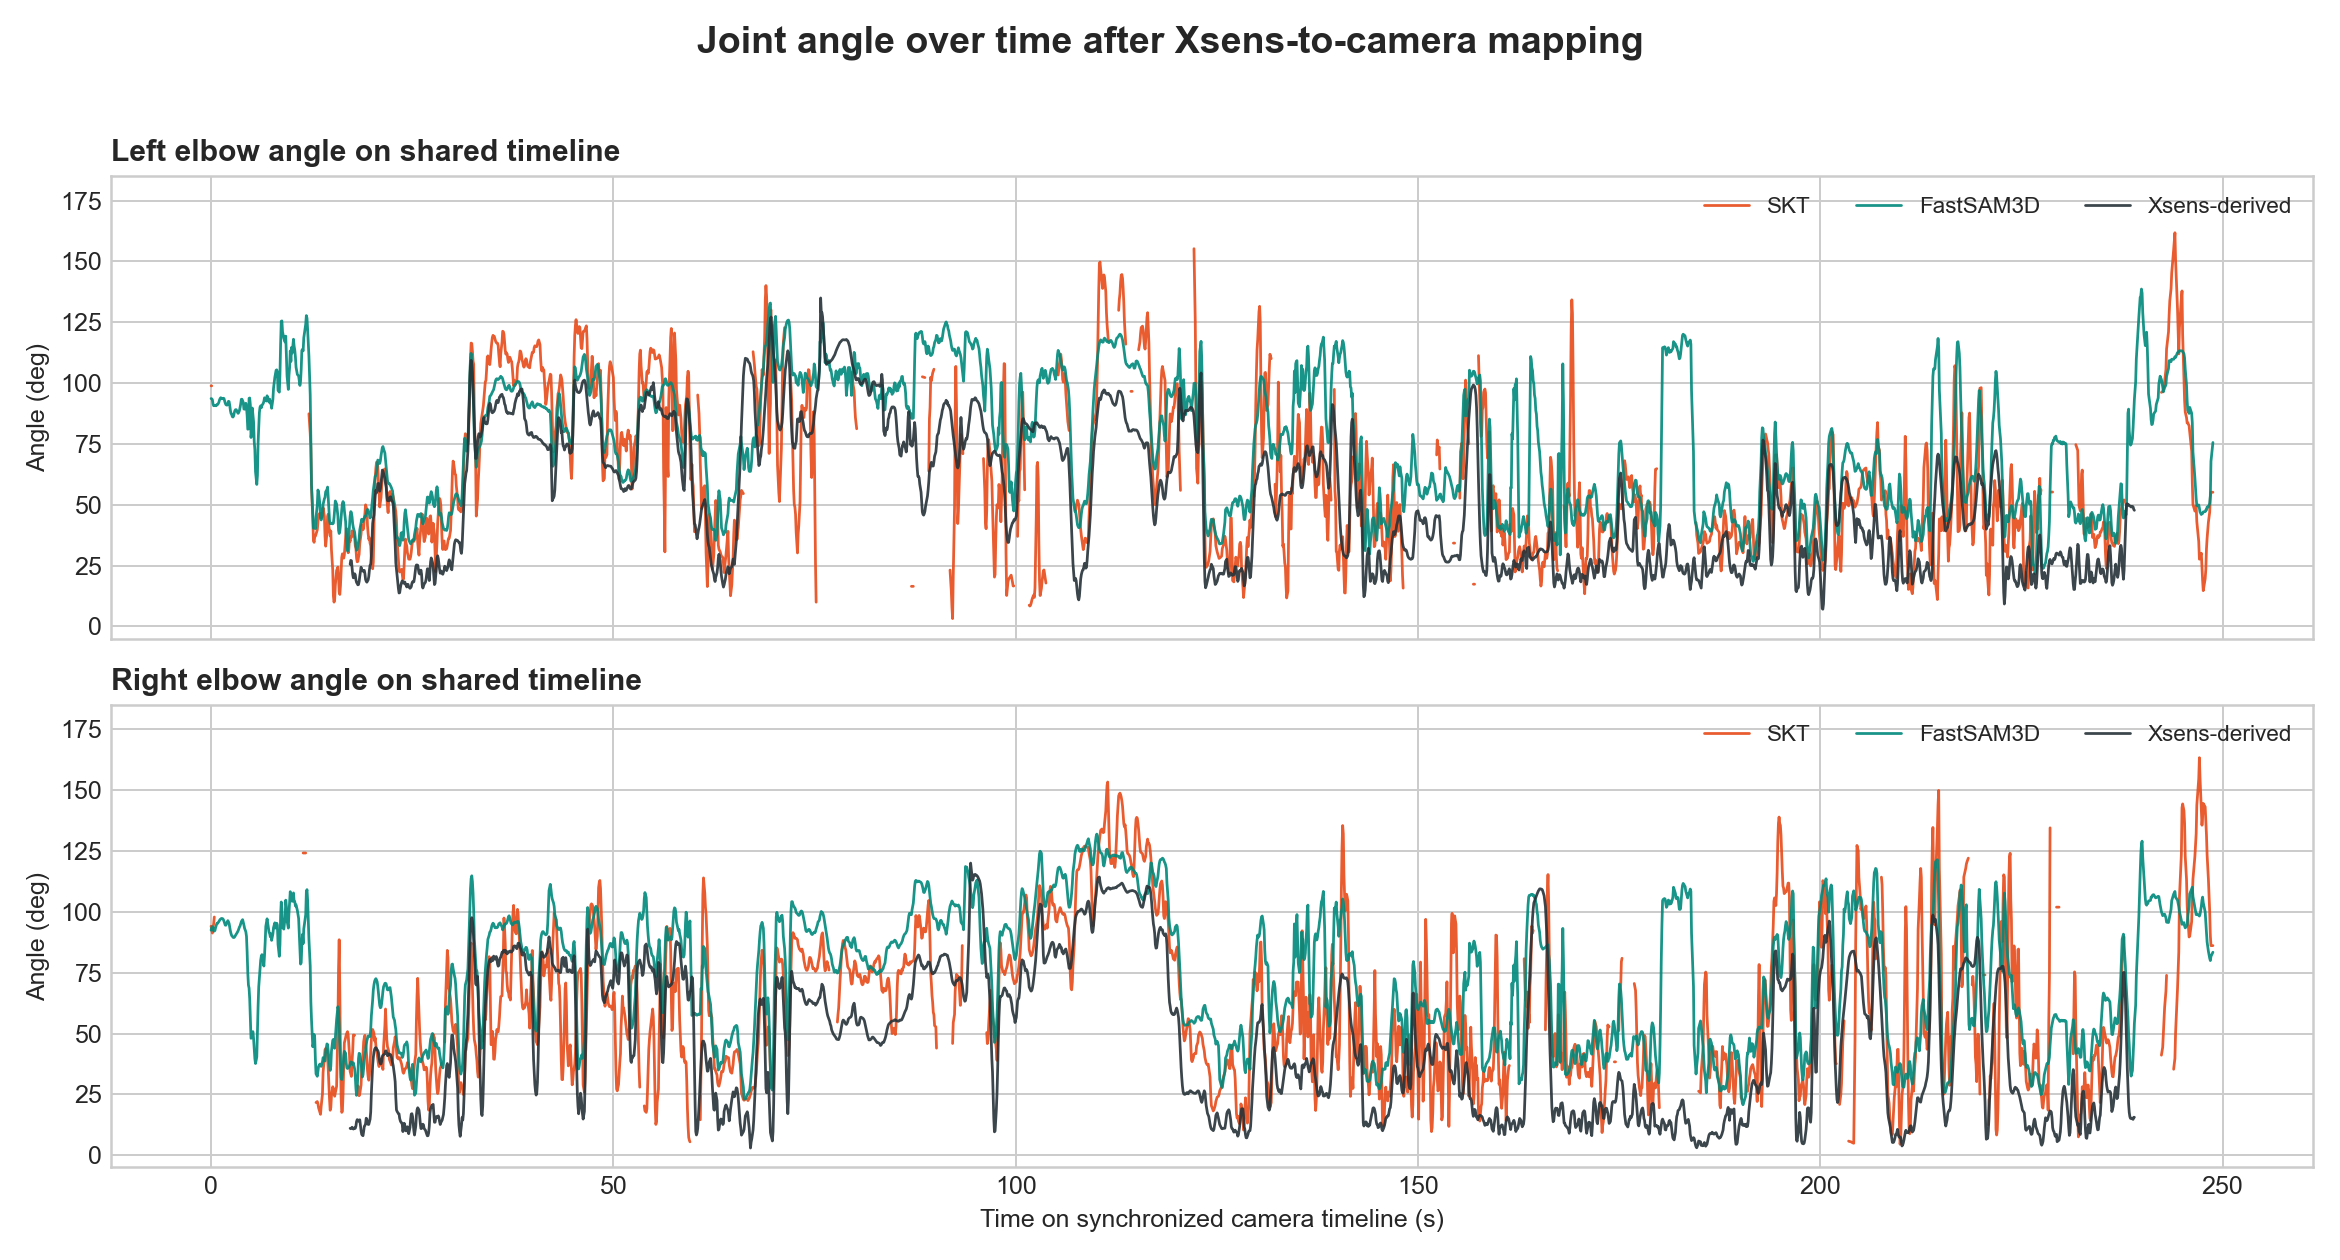
\includegraphics[width=\linewidth]{thesis_joint_angle_over_time.png}
  \caption{Left and right elbow angles on the shared timeline after offset correction. The plot provides a qualitative synchronisation check before quantitative angle and motion metrics are interpreted.}
  \label{fig:angle_time_alignment}
\end{figure}

A third check addresses the possibility that, even with a near-perfect
mean offset, the camera and Xsens clocks could drift slowly over the
$\sim$4\,min recording.
Figure~\ref{fig:first_last_delta} compares the K=6 motion-delta windows at
the beginning and end of the common valid interval; had the underlying
drift been large, the late-interval deltas would be expected to lose their
alignment with the reference even though the early-interval deltas still
agree.
The check is qualitative rather than a formal drift estimate, but the
observed late-interval agreement is comparable to the early-interval
agreement, which supports the use of a single constant offset for the
remainder of the thesis while explicitly acknowledging that future longer
or multi-take recordings should repeat this check.

\begin{figure}[!htbp]
  \centering
  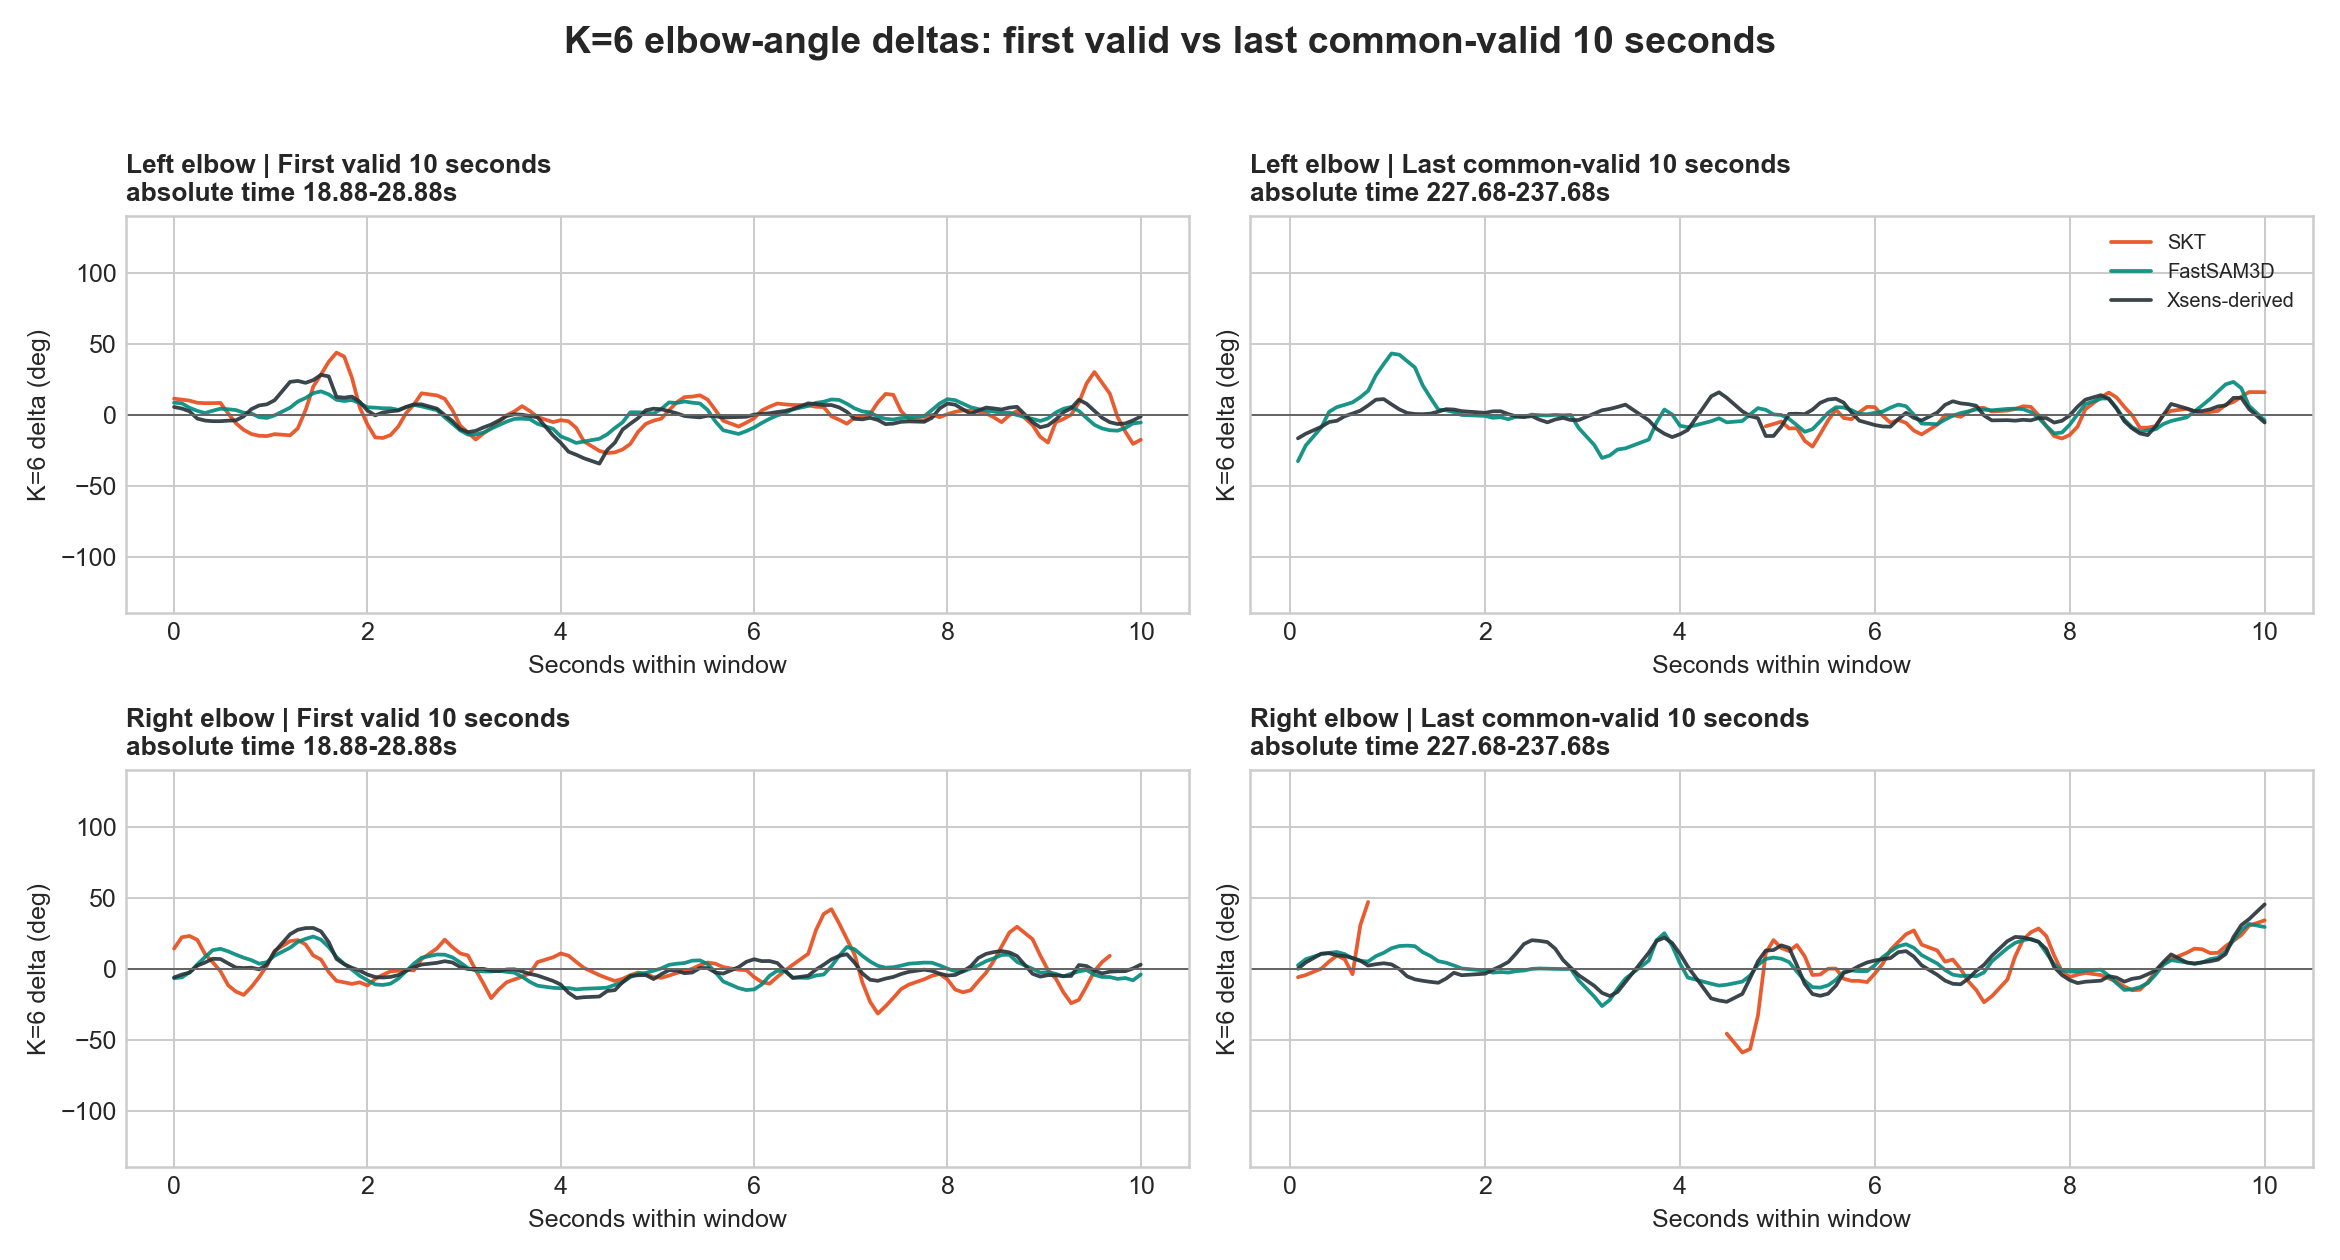
\includegraphics[width=\linewidth]{thesis_k6_delta_first_last_10s.png}
  \caption{K=6 elbow motion deltas near the beginning and end of the common valid interval. This figure is used as a practical check that the chosen constant offset remains reasonable across the recording.}
  \label{fig:first_last_delta}
\end{figure}

\clearpage
% =============================================================
\section{Methods}
\label{sec:methods}
% =============================================================

\subsection{Overview}

The thesis benchmarks two pose-estimation pipelines against the same Xsens
reference and the same evaluation protocol: SKT, the primary calibrated
sparse-stereo method developed in this thesis, and FastSAM3D, the monocular
learning-based alternative.
Figure~\ref{fig:pipeline_overview} shows the full experimental flow, and
Table~\ref{tab:method_roles} summarises each pipeline's input assumption, main
advantage, and main risk.

The single design choice that matters most for interpreting the rest of the
thesis is the deliberate separation between pose estimation and evaluation.
Both methods are mapped onto the same shared timeline and judged with
the same metrics, but those metrics are then split across two independent
axes (angle, motion) rather than collapsed into a single ranking
score; this prevents the recurring failure mode in which a method that is
strong in one space, for example metric stereo geometry, is implicitly
assumed to be equally strong in temporal angle consistency.

\begin{figure}[!htbp]
  \centering
  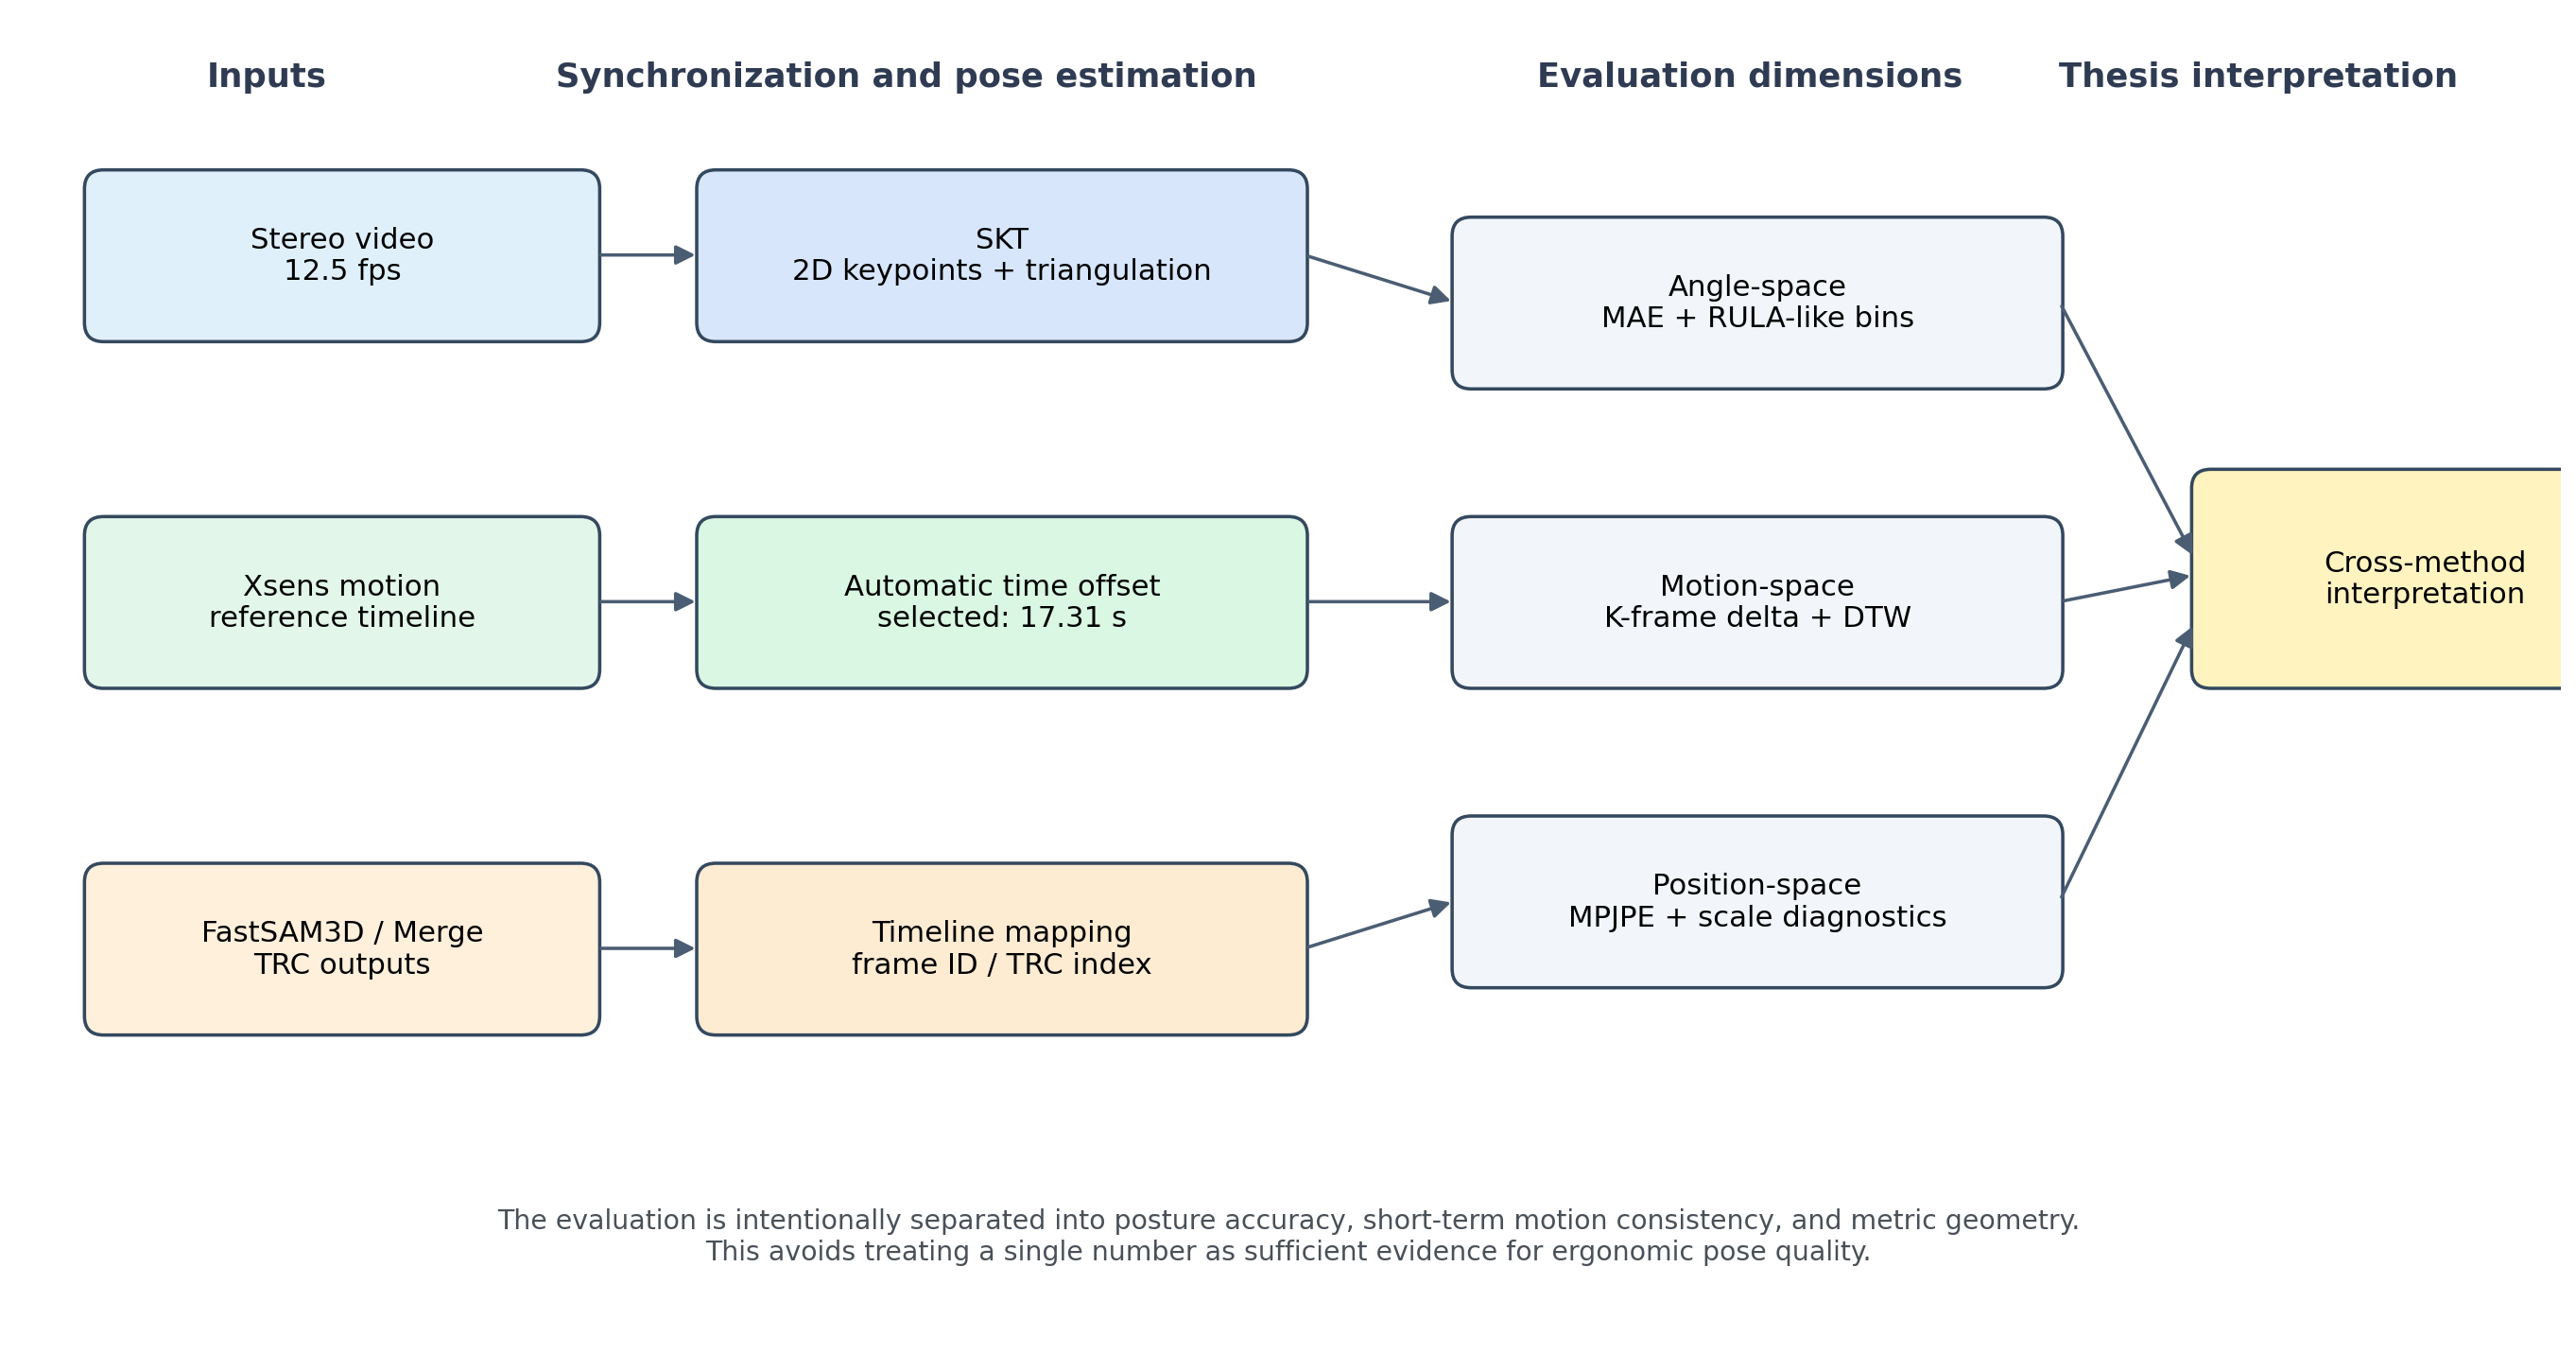
\includegraphics[width=\linewidth]{thesis_pipeline_overview.png}
  \caption{Overview of the thesis evaluation pipeline. Inputs are synchronized and evaluated separately in angle space, motion space, and position space before the final cross-method interpretation.}
  \label{fig:pipeline_overview}
\end{figure}

\begin{table}[!htbp]
  \centering
  \caption{Role of each evaluated pose-estimation path in the thesis.}
  \label{tab:method_roles}
  \small
  \begin{tabularx}{\linewidth}{lXXX}
    \toprule
    Method & Input assumption & Main advantage & Main risk \\
    \midrule
    SKT
    & Synchronized stereo video and calibrated cameras
    & Metric 3D scale and explicit geometric quality signals
    & 2D keypoint jitter and left--right mismatch are amplified by triangulation \\
    FastSAM3D
    & Monocular pose output provided as TRC markers
    & Learned body/motion priors give stable angle and motion behaviour
    & Coordinate, scale, and keypoint semantics require careful interpretation \\
    \bottomrule
  \end{tabularx}
\end{table}

\subsection{Sparse Keypoint Triangulation (SKT)}

The primary method developed in this thesis, Sparse Keypoint Triangulation
(SKT), turns a calibrated stereo video pair into a 3D body skeleton through
a transparent geometric chain that exposes per-frame quality signals at
every stage.
For each synchronised left/right frame pair, the pipeline first runs a 2D
human pose detector on each view to obtain 17 COCO-format keypoints with
per-keypoint confidence; the two views' keypoints are then matched by
keypoint index and filtered by three geometric consistency checks
(minimum triangulation confidence, maximum epipolar error, maximum
reprojection error after triangulation); the surviving pairs are
triangulated into 3D coordinates through the Direct Linear Transform
applied to the calibrated projection matrices; and finally the joint
angles are computed from triplets of 3D keypoints using the same
three-point arccosine formula that is applied to the Xsens-derived
geometric reference.

The methodological reason for building SKT this way -- rather than, for
example, regressing 3D pose directly with a learned model -- is
interpretability under deployment.
Every 3D point in an SKT output is tied to two observed 2D detections and
to a known stereo calibration model, so the pipeline can expose a set of
geometry-aware quality signals (triangulation confidence, epipolar error,
reprojection error, disparity) that downstream ergonomic monitoring can
use as a per-frame trust score; unreliable frames can therefore be
detected and gated rather than silently converted into ergonomic risk
scores, which is a property no end-to-end learned regressor offers for
free.
The corresponding methodological cost is that each SKT 3D point inherits
the noise of its 2D detections in both views; small 2D jitter is first
amplified by triangulation and then further amplified by joint-angle
computation, so SKT is most usefully understood as a measurement pipeline
whose output should be read together with its quality signals rather than
as a smoothed motion sequence.

This view of SKT as a measurement pipeline -- rather than a black-box
reconstruction module -- is also what motivates the later motion-delta
evaluation.
When a wrist or elbow keypoint is detected inconsistently between the two
views, the resulting 3D joint can remain numerically valid (the rays still
intersect, the reprojection is still small) while producing a sharply
different triangulated angle from the surrounding frames, which appears in
later analysis as occasional large motion deltas concentrated near
elbow-chain instabilities.
Section~\ref{sec:discussion} returns to these high-delta cases as concrete
failure evidence rather than treating them as generic noise.

\subsection{FastSAM3D (Monocular Learning Baseline)}

FastSAM3D is included as the learning-based monocular counterpart to SKT
and is the most informative single comparison in the thesis, because it
keeps the same input modality (the camera) but replaces multi-view
geometry with learned body-shape and motion priors.
Instead of triangulating left/right keypoint pairs, FastSAM3D produces a
3D pose directly from one camera stream through a model-based pipeline
that combines fast instance segmentation with learned body-shape and pose
priors \cite{yang2026fastsam3d}; the specific FastSAM3D
implementation is treated here as an externally produced output, and its
results are delivered as TRC marker files that are re-mapped to the
COCO-17 keypoint convention and resampled onto the shared camera timeline
before any evaluation metric is computed.

The methodological reason to include FastSAM3D is that learned body-shape
and motion priors should, in principle, smooth out the per-frame keypoint
noise that hurts SKT, because the learned model implicitly enforces
anatomically consistent transitions between consecutive poses even without
explicit multi-view evidence.
The corresponding methodological cost is that the FastSAM3D output does
not necessarily share the SKT coordinate frame, scale convention, or
exact keypoint semantics; FastSAM3D is therefore evaluated primarily in
the angle and motion axes, where these conventions cancel, while
position-space results are reported only as coordinate/scale diagnostics
rather than as direct pose-quality scores.

\clearpage
% =============================================================
\section{Evaluation Framework}
\label{sec:evaluation}
% =============================================================

\subsection{Angle-space Evaluation}

The angle-space track answers the most direct question for ergonomic
deployment -- ``Is the estimated joint posture quantitatively close to
the reference?'' -- and it is therefore reported first in every per-method
analysis even though it is the axis most exposed to the Xsens calibration
limitation discussed in Section~\ref{sec:background}.
Eight full-body angles are evaluated, covering the four bilateral joints
that drive most of the RULA assessment: left and right shoulder, elbow,
hip, and knee flexion.
To remove angle-definition mismatch between systems, every angle is
computed from the same three-point geometric formula applied to the
relevant triplet of 3D keypoints, both for the vision methods and for the
Xsens-derived geometric reference:
\begin{equation}
  \theta = \arccos\!\left(
    \frac{(\mathbf{p}_A-\mathbf{p}_B)\cdot(\mathbf{p}_C-\mathbf{p}_B)}
         {\|\mathbf{p}_A-\mathbf{p}_B\|\;\|\mathbf{p}_C-\mathbf{p}_B\|}
  \right).
\end{equation}
The main reported metrics are mean absolute error (MAE), median absolute
error, bias (signed mean error), valid-pair ratio, and -- as the
application-level companion -- RULA-like bin agreement for the
upper-body joints.

\subsection{Motion-space Evaluation}

The motion-space track is the thesis's principal countermeasure against
the Xsens calibration offset: it asks whether two systems describe the
\emph{same change in posture} rather than the same absolute posture, so
that any static reference offset cancels out by differencing.
For a given time scale $K$, the K-frame angle delta is defined as
\begin{equation}
  \Delta_K \theta_t \;=\; \theta_t \;-\; \theta_{t-K},
\end{equation}
and the thesis evaluates four time scales, $K\in\{1,6,12,25\}$ frames
(approximately 0.08, 0.48, 0.96, and 2.00\,s at 12.5\,fps), to probe the
agreement across genuinely instantaneous changes, sub-second sub-actions,
1\,s smooth-motion windows, and 2\,s near-action-level windows.
K=6 is adopted as the main reporting and visualisation scale because it
corresponds to a $\sim$0.48\,s sub-action -- short enough to remain a
true motion-level metric, long enough to suppress per-frame keypoint
jitter -- while the K=1 and K=25 numbers provide context as the
noise-dominated and amplitude-dominated extremes.
Reported metrics include Pearson correlation, Spearman rank correlation,
delta MAE and RMSE, high-delta count, and the path ratio (cumulative
absolute target delta divided by cumulative absolute reference delta),
which together separate ``shape agreement'' from ``amplitude agreement''
in the motion signal.

\subsection{Segment-level Evaluation}

The segment-level track condenses the frame-level motion comparison into
a small set of physically interpretable active-movement intervals,
because reporting only frame-level metrics tends to hide whether a method
captures the actual movement bursts that ergonomic risk assessment cares
about.
Activity segments are detected from the reference signal as contiguous
intervals of sustained K-frame motion above a threshold, and for each
segment four numbers are reported per method: range of motion (ROM,
max-min angle), per-segment angle MAE, RULA-like bin agreement based on
the segment's peak angle, and a dynamic time warping (DTW) distance
\cite{sakoe1978dtw}.
The DTW comparison is run on \emph{mean-subtracted and L2-normalised}
per-segment angle sequences, following the practice that has been
recommended for human-motion shape comparison in the recent literature
\cite{perezluque2026reaching}; the normalisation deliberately removes
absolute offset and amplitude so that DTW measures whether the
\emph{shape of motion through the segment} is similar, making it
complementary to MAE/RMSE (which measure amplitude error) rather than
redundant with them.

\subsection{Position-space Evaluation}

The position-space track does not compete with the angle and motion
tracks for ``best pose method'' -- it answers a separate deployment
question: ``Which method produces 3D coordinates whose scale and
geometry can be trusted in a metric workspace?''
For SKT, calibrated stereo geometry gives the coordinates an inherent
metric scale, so MPJPE-style distances and pelvis-relative comparisons
can be reported directly after rigid alignment using the standard Kabsch
estimator \cite{kabsch1976solution}.
For FastSAM3D, the output coordinate frame and scale convention do not
necessarily match the stereo or Xsens frames, so position-space numbers
must be reported with explicit alignment provenance; the thesis uses
position-space results primarily to (i) demonstrate stereo's
metric-scale advantage and (ii) document the coordinate/scale work that
any monocular pipeline must do before its 3D output becomes deployable.

\subsection{Filtering Policy}

The evaluation tracks above are well-defined only if the per-system
filtering policy is itself controlled, because temporal smoothing
applied at different strengths to different systems can quietly inflate
or deflate motion-space agreement without changing any reported number
in an obvious way.
The thesis therefore adopts a deliberate per-system policy.
Xsens streams are interpolated onto the shared timeline but are
\emph{not} re-smoothed by the project, because the Xsens internal
processing already includes substantial filtering, and stacking a
project-side filter on top would silently double the smoothing on
the reference side of every comparison.
The camera-based methods are smoothed with a single light moving-average
filter whose window is recorded in the run configuration; the chosen
window represents a $\sim$200\,ms low-lag setting consistent with empirical
guidance for human upper-body motion signals \cite{perezluque2026reaching}.
The single methodological invariant that must hold across all runs is
that smoothing is always applied \emph{before} delta computation, since
the opposite order would let the delta metric measure filter artifacts
rather than the underlying motion signal.

\begin{table}[!htbp]
  \centering
  \caption{Interpretation of the evaluation tracks used in the thesis.}
  \label{tab:evaluation_tracks}
  \small
  \begin{tabularx}{\linewidth}{lXXX}
    \toprule
    Track & Question answered & Main metrics & Main caveat \\
    \midrule
    Angle-space
    & Is the posture suitable for ergonomic angle interpretation?
    & MAE, median AE, bias, valid ratio, RULA-like bin agreement
    & Sensitive to reference-system angle definitions and static offsets \\
    Motion-space
    & Do two systems describe the same short-term movement?
    & K-frame delta correlation, delta MAE, RMSE, high-delta count, DTW
    & Requires careful time alignment and consistent smoothing policy \\
    Segment-level
    & Are active movement intervals similar in range and shape?
    & ROM error, segment MAE, DTW distance, RULA-like agreement
    & Depends on segment detection thresholds and valid-frame coverage \\
    Position-space
    & Are reconstructed 3D skeletons geometrically compatible?
    & MPJPE, pelvis-relative distance, aligned inter-method distance
    & Monocular methods may use different coordinate and scale conventions \\
    \bottomrule
  \end{tabularx}
\end{table}

This separation is central to the thesis argument.
For example, a method can produce good angle trends while still being
difficult to compare in absolute 3D coordinates, or it can preserve metric
scale while producing jittery short-term angles.
The evaluation framework therefore reports multiple complementary quantities
instead of selecting a single ``winner'' metric.

\clearpage
% =============================================================
\section{Results}
\label{sec:results}
% =============================================================

\subsection{Angle-space Results}

In the angle-space track, the monocular learning-based FastSAM3D pipeline
outperforms SKT, but the margin is small enough that the result must be
read with the Xsens reference-system caveat in mind rather than as a
universal verdict.
Averaged across the eight evaluated joint angles, FastSAM3D reaches a mean
MAE of 15.4\degr\ against the Xsens-derived reference, compared with
17.6\degr\ for SKT; the corresponding median MAEs (14.4\degr\ vs.\
17.9\degr) preserve the same ranking, and FastSAM3D also has the higher
valid-pair ratio (0.905 vs.\ 0.746).
The Xsens-native check sits at 4.7\degr\ MAE, an order of magnitude below
the vision methods, and is reported in the same table only as a
reference-system internal anchor rather than as a competing pose method.

The most informative joint-level pattern is that the per-joint MAE
ranking is not flat across the eight angles.
Shoulder, hip, and knee angles dominate FastSAM3D's lead, where its
learned body priors stabilise the chain endpoints; the elbow is the
hardest joint for every vision method, in line with the long
shoulder--elbow--wrist chain that amplifies both keypoint noise (for SKT)
and pose-prior uncertainty (for FastSAM3D), and this is the joint where
both methods are penalised most by the Xsens calibration offset
itself.
For this reason the elbow is the joint that drives the motion-space
analysis that follows -- angle MAE alone cannot tell which fraction of
the elbow error is genuine pose error and which fraction is reference
offset.

\begin{table}[!htbp]
  \centering
  \caption{Angle-space summary across eight evaluated joint angles. Lower MAE is better.}
  \label{tab:angle_summary}
  \small
  \begin{tabular}{lcccc}
    \toprule
    Method & Mean MAE $\downarrow$ & Median MAE $\downarrow$ &
    Valid ratio $\uparrow$ & Bin agreement $\uparrow$ \\
    \midrule
    SKT & 17.6 & 17.9 & 0.746 & 0.540 \\
    \good{FastSAM3D} & \good{15.4} & \good{14.4} & \good{0.905} & \good{0.553} \\
    \textit{Xsens native check} & \textit{4.7} & \textit{3.7} & \textit{0.905} & \textit{0.886} \\
    \bottomrule
  \end{tabular}
\end{table}

Figure~\ref{fig:angle_summary_plot} visualises the same comparison.
The bar plot is included precisely because the FastSAM3D--SKT gap is
small and consistent rather than large and dramatic; a single bar
that was twice as high as another would not survive any reasonable
sensitivity check on this single recording, whereas a small but
systematic gap is the more honest evidence on which to base the
discussion of learned pose priors later in the thesis.

\begin{figure}[!htbp]
  \centering
  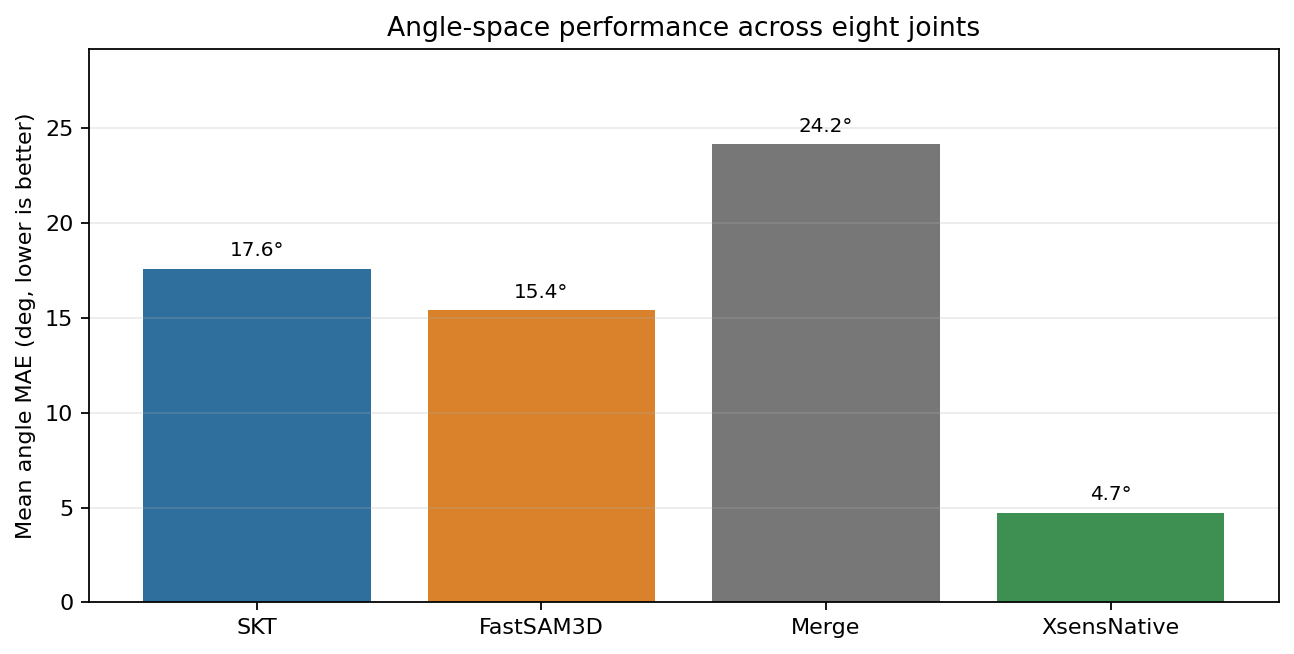
\includegraphics[width=0.92\linewidth]{thesis_angle_summary.png}
  \caption{Angle-space summary across evaluated methods. FastSAM3D has the lowest mean and median MAE among the vision methods, while the Xsens-native check indicates the approximate lower bound of the reference-system representation difference.}
  \label{fig:angle_summary_plot}
\end{figure}

\subsection{Motion-space Results}

In the motion-space track, the FastSAM3D advantage observed in absolute
angles becomes both clearer and easier to interpret, because differencing
the angle sequences cancels the Xsens calibration offset that confounded
the angle-space comparison.
Averaged across the eight evaluated angles at $K=6$ frames ($\sim$0.48\,s),
FastSAM3D reaches a mean Pearson correlation of 0.64 with the Xsens-derived
reference, against 0.38 for SKT; the corresponding mean Spearman rank
correlations (0.64 vs.\ 0.33) preserve the same ranking, which rules out
the explanation that FastSAM3D is winning only because of a handful of
high-amplitude points that inflate Pearson without lifting the rank
correlation.
At the elbow -- the joint that the motion-space track is designed to
adjudicate -- FastSAM3D reaches Pearson correlations of 0.54 (left) and
0.69 (right) against SKT's 0.39 / 0.39, a comparable shape-agreement gap
on the joint that the angle-space analysis flagged as ambiguous.
The Xsens-native check returns the expected $\sim$0.96 mean correlation,
confirming that the K=6 metric can recover near-perfect agreement when
the two compared signals genuinely measure the same motion.

\begin{table}[!htbp]
  \centering
  \caption{K=6 motion-delta agreement. Higher correlation is better.}
  \label{tab:motion_summary}
  \small
  \begin{tabular}{lcccc}
    \toprule
    Method & Mean $r$ $\uparrow$ & Mean $\rho$ $\uparrow$ &
    L-elbow $r$ $\uparrow$ & R-elbow $r$ $\uparrow$ \\
    \midrule
    SKT & 0.379 & 0.334 & 0.392 & 0.386 \\
    \good{FastSAM3D} & \good{0.644} & \good{0.635} & \good{0.542} & \good{0.689} \\
    \textit{Xsens native check} & \textit{0.965} & \textit{0.936} & \textit{0.988} & \textit{0.993} \\
    \bottomrule
  \end{tabular}
\end{table}

Figure~\ref{fig:motion_k6_summary_plot} visualises the K=6 correlation
summary and makes the main finding immediately legible: FastSAM3D is
consistently above SKT across the eight evaluated angles, and the Xsens-native
check provides the visual upper bound that anchors the scale of the plot.
The per-elbow scatter plots in Figure~\ref{fig:k6_elbow_scatter} then make
the same comparison at the frame level rather than the summary level:
FastSAM3D's scatter clusters along the ideal diagonal with limited vertical
spread, whereas SKT's scatter shows a recurring vertical accumulation near
zero reference delta -- the geometric signature of high SKT delta values
during physically quiet intervals, which Section~\ref{sec:discussion}
traces back to localised keypoint-chain instability rather than to a
constant noise floor.

\begin{figure}[!htbp]
  \centering
  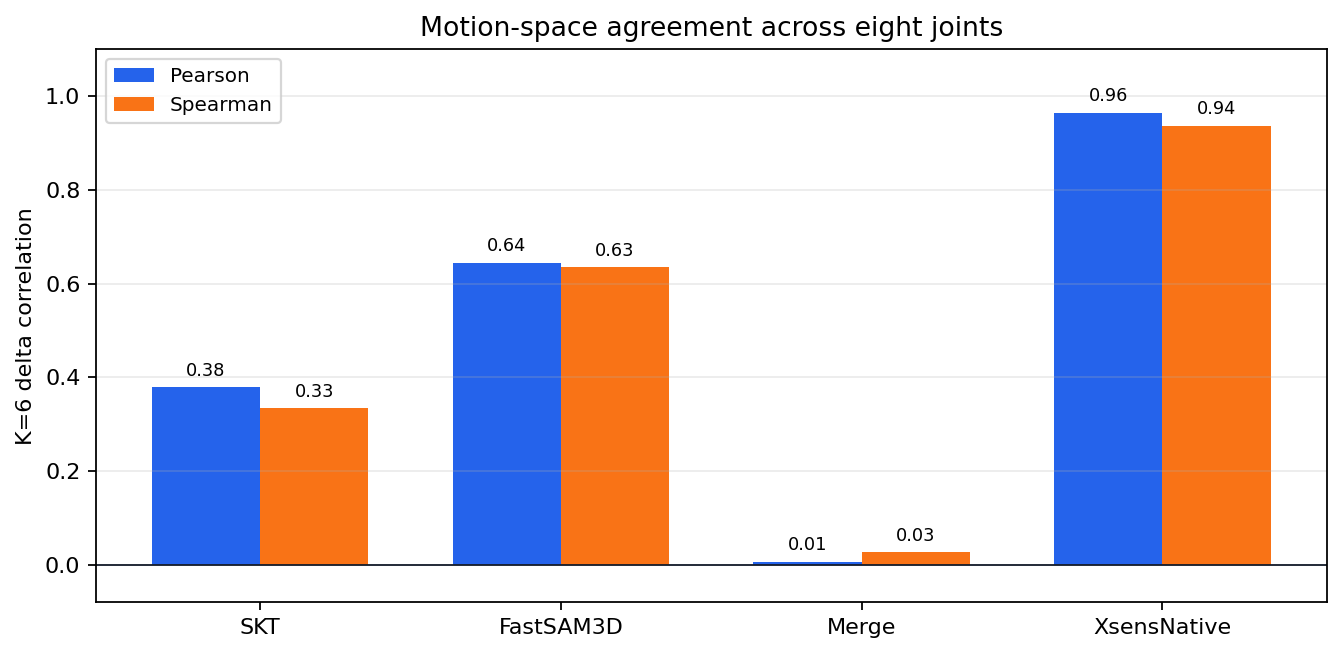
\includegraphics[width=0.92\linewidth]{thesis_motion_k6_summary.png}
  \caption{K=6 motion-delta correlation summary. FastSAM3D shows stronger short-term motion agreement than SKT on the current dataset.}
  \label{fig:motion_k6_summary_plot}
\end{figure}

\begin{figure}[!htbp]
  \centering
  \begin{subfigure}[b]{0.48\linewidth}
    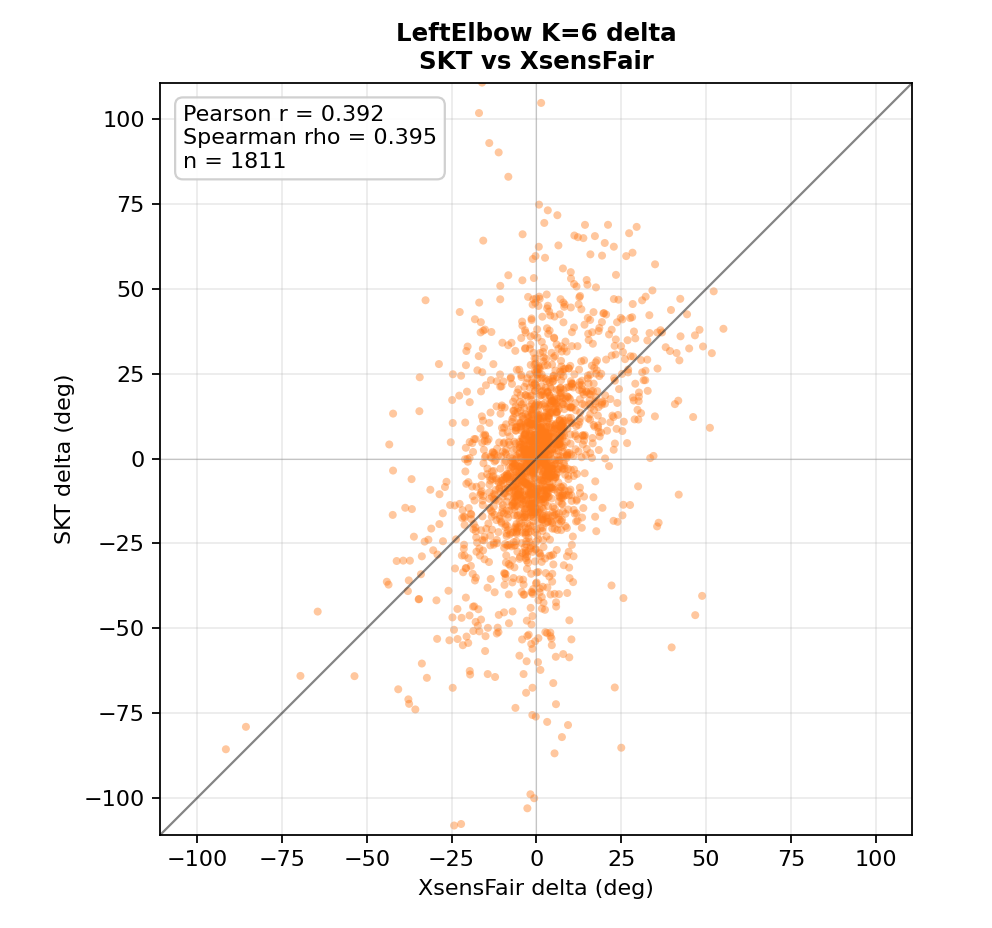
\includegraphics[width=\linewidth]{thesis_scatter_skt_vs_xsensfair_leftelbow_k6.png}
    \caption{SKT, left elbow.}
  \end{subfigure}
  \hfill
  \begin{subfigure}[b]{0.48\linewidth}
    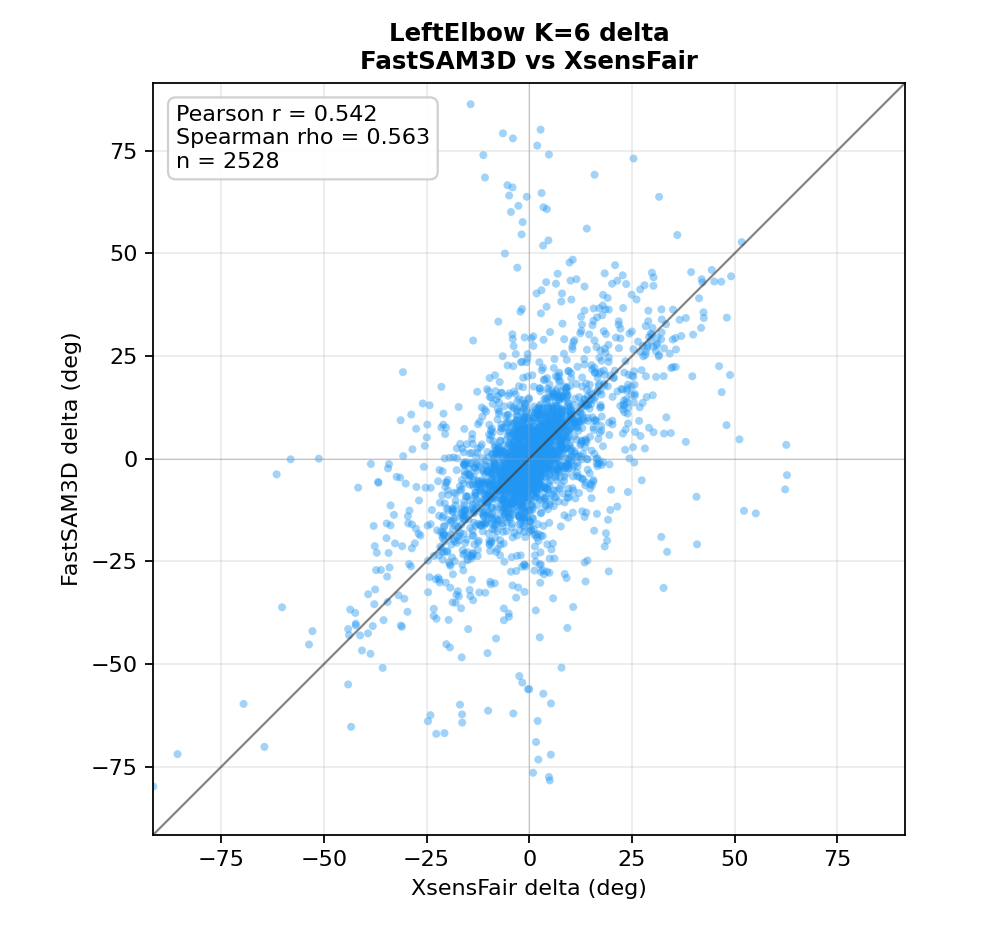
\includegraphics[width=\linewidth]{thesis_scatter_fastsam3d_vs_xsensfair_leftelbow_k6.png}
    \caption{FastSAM3D, left elbow.}
  \end{subfigure}

  \vspace{0.4cm}
  \begin{subfigure}[b]{0.48\linewidth}
    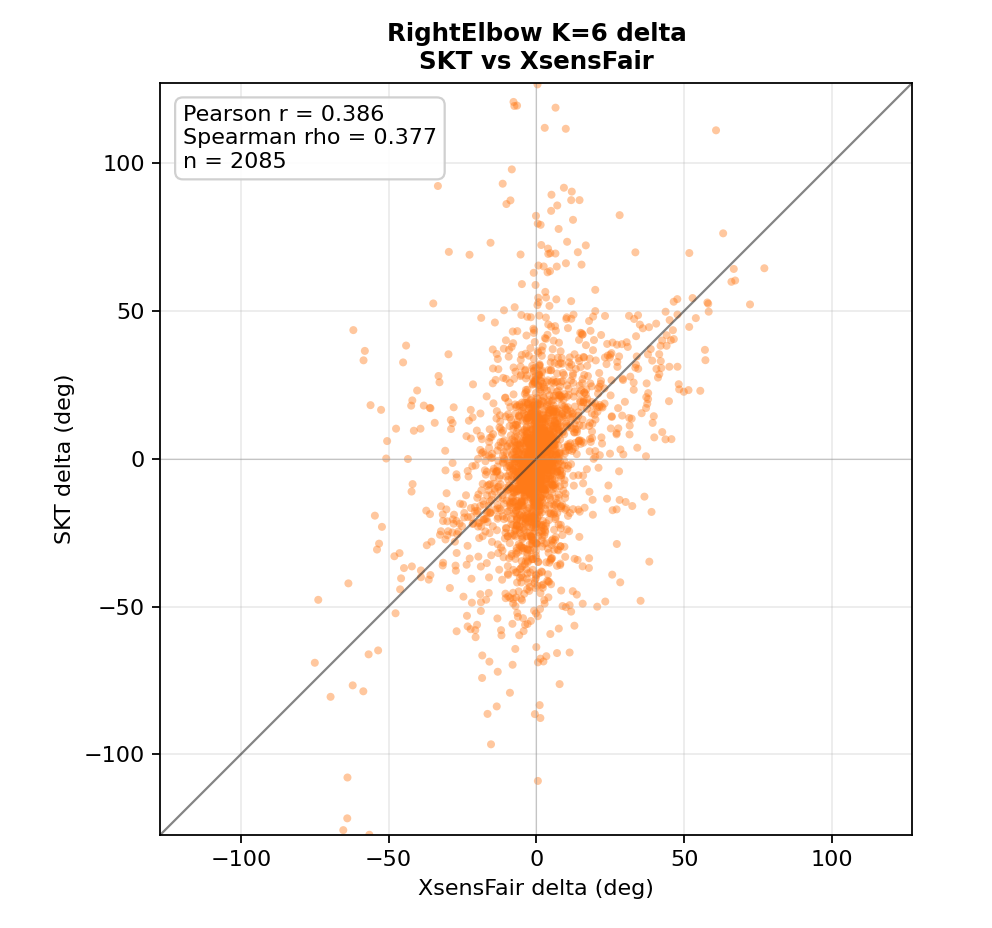
\includegraphics[width=\linewidth]{thesis_scatter_skt_vs_xsensfair_rightelbow_k6.png}
    \caption{SKT, right elbow.}
  \end{subfigure}
  \hfill
  \begin{subfigure}[b]{0.48\linewidth}
    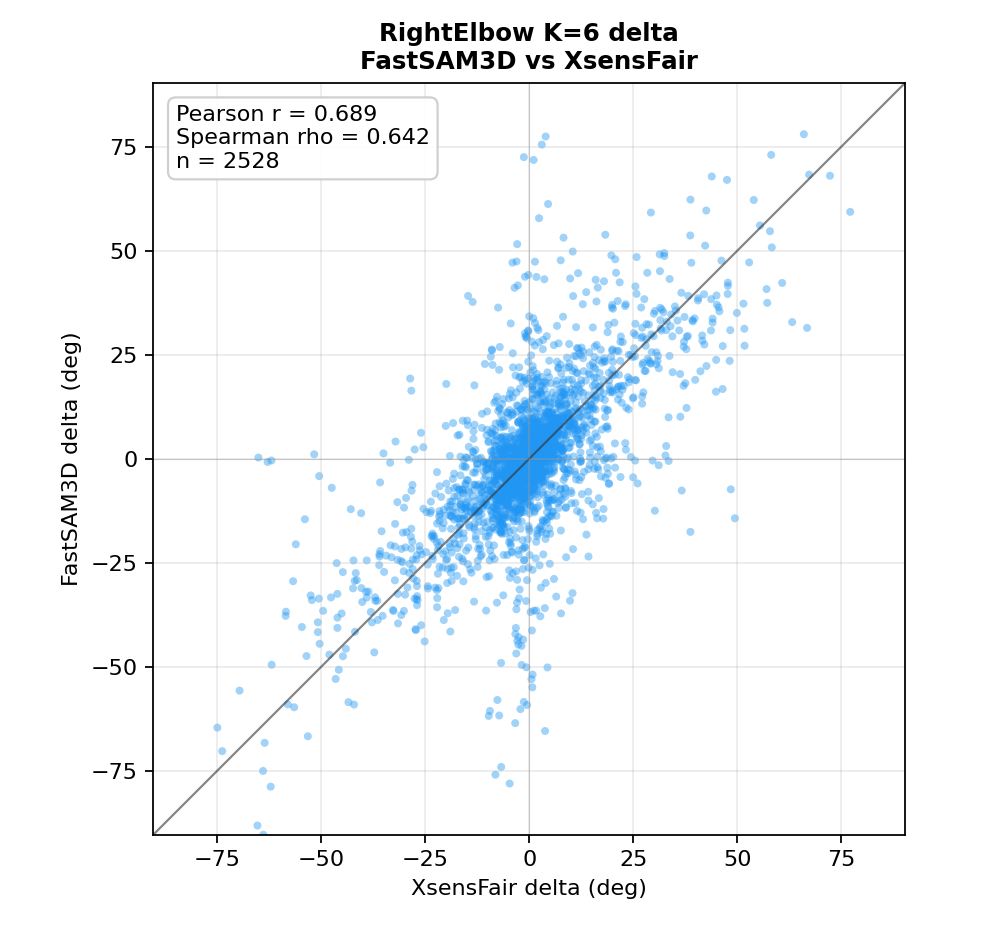
\includegraphics[width=\linewidth]{thesis_scatter_fastsam3d_vs_xsensfair_rightelbow_k6.png}
    \caption{FastSAM3D, right elbow.}
  \end{subfigure}
  \caption{K=6 elbow motion-delta scatter plots against the Xsens-derived reference. FastSAM3D follows the ideal trend more consistently, while SKT shows more high-delta jitter and vertical-axis accumulation.}
  \label{fig:k6_elbow_scatter}
\end{figure}

The sensitivity of the motion-space ranking to the chosen time scale is
shown in Figure~\ref{fig:pearson_vs_k}.
At $K=1$ (single-frame deltas, $\sim$80\,ms) every vision method's
correlation drops because the metric is dominated by per-frame keypoint
jitter that is roughly uncorrelated with the reference; at $K=25$
($\sim$2\,s) every vision method's correlation rises because the metric
is approaching an amplitude-of-motion comparison rather than a true
short-term agreement.
The thesis adopts $K=6$ as the main reporting point because it lies on
the elbow of these two trends: it suppresses single-frame keypoint noise
without smoothing across a complete action, so the ranking it produces
remains a genuine motion-agreement statement rather than either a
noise floor or a re-statement of segment-level ROM.

\begin{figure}[!htbp]
  \centering
  \begin{subfigure}[b]{0.48\linewidth}
    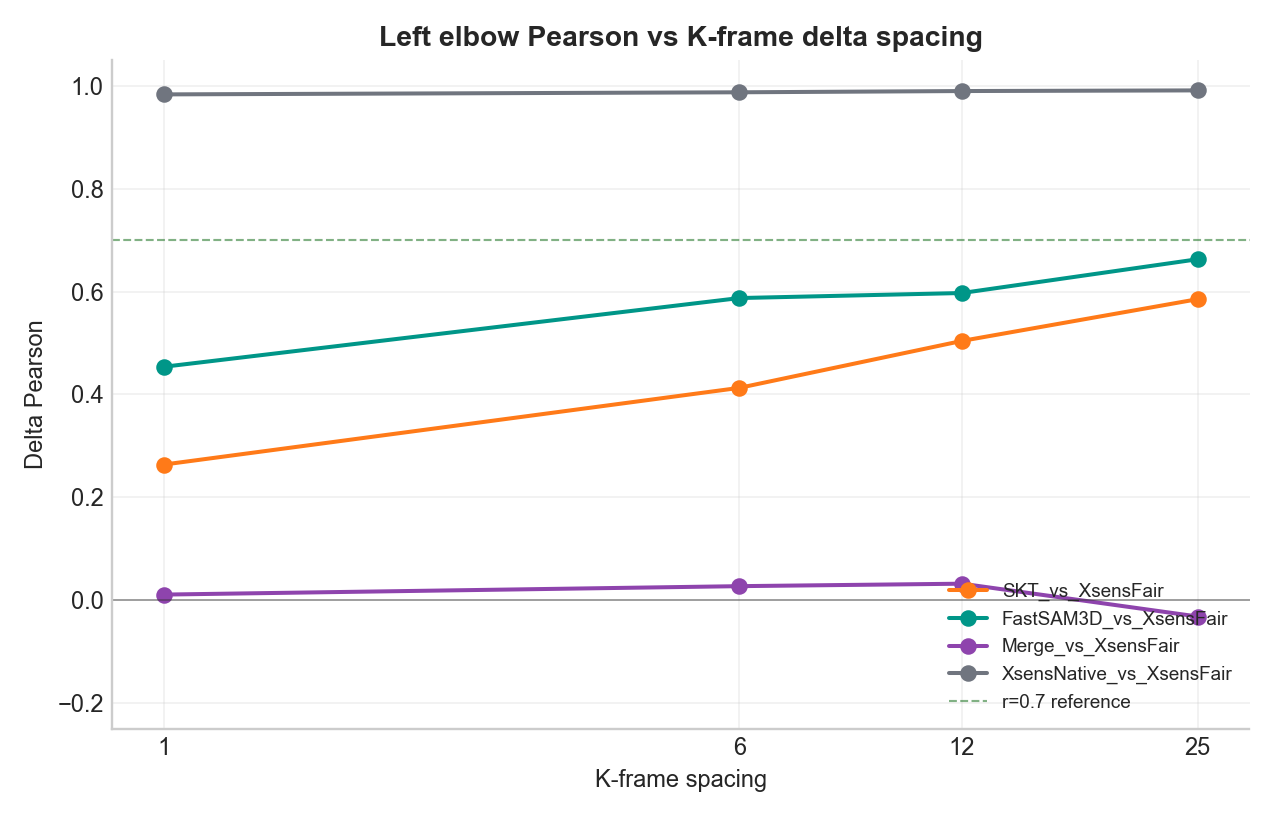
\includegraphics[width=\linewidth]{thesis_pearson_vs_k_leftelbow.png}
    \caption{Left elbow.}
  \end{subfigure}
  \hfill
  \begin{subfigure}[b]{0.48\linewidth}
    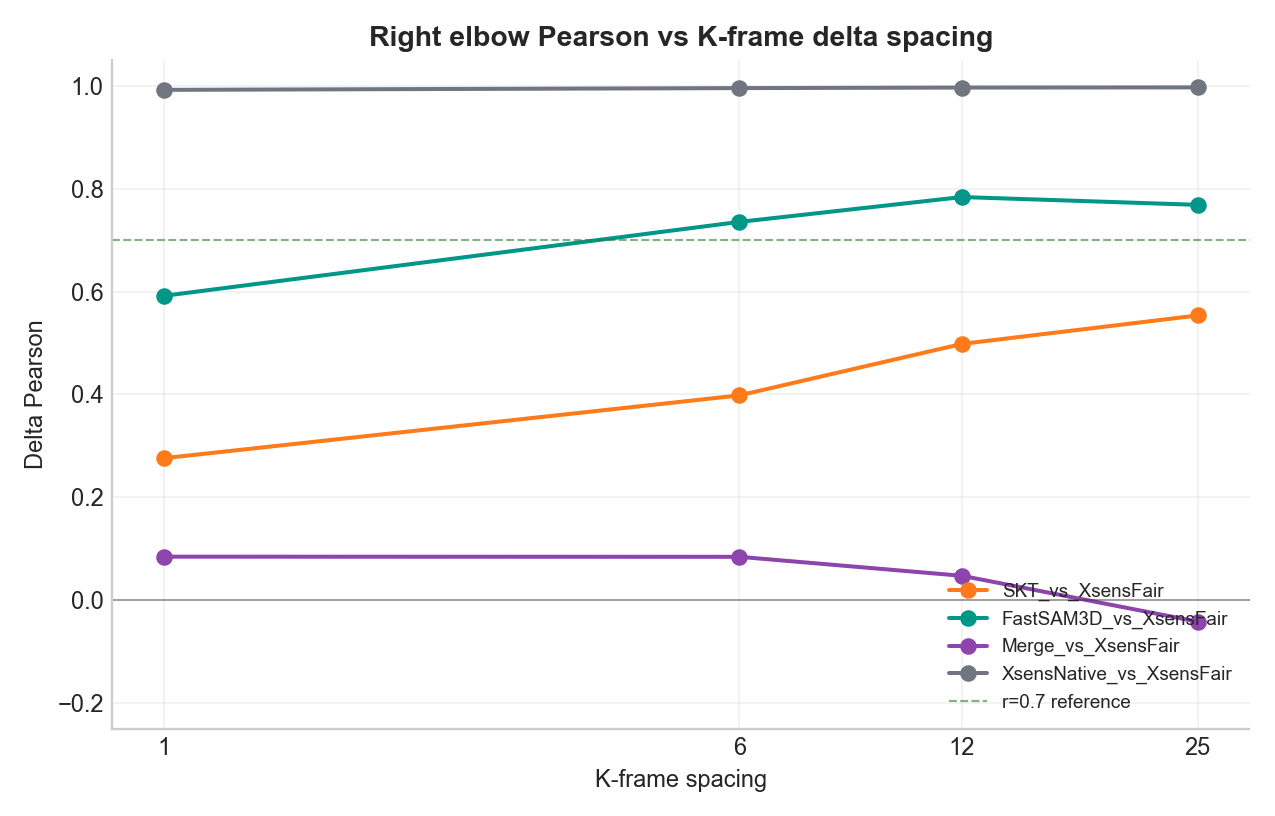
\includegraphics[width=\linewidth]{thesis_pearson_vs_k_rightelbow.png}
    \caption{Right elbow.}
  \end{subfigure}
  \caption{Motion-delta correlation as a function of K. The result supports using K=6 as a practical compromise between jitter sensitivity and motion interpretability.}
  \label{fig:pearson_vs_k}
\end{figure}

\subsection{Segment-level Results}

The segment-level track reinforces the frame-level motion finding while
adding two pieces of information that the frame-level numbers alone cannot
provide: per-segment range-of-motion (ROM) error in degrees, which is the
quantity most directly comparable to a ``movement size'' an ergonomist
would estimate manually, and per-segment normalised DTW distance, which
quantifies how similar the shape of motion through each segment is once
amplitude and offset are removed.
Aggregated over the detected active segments (39 for SKT, 45 for
FastSAM3D), FastSAM3D has both the lower mean ROM error (14.9\degr\ vs.\
26.9\degr\ for SKT) and the lower mean DTW distance (0.0355 vs.\ 0.0435).
The Xsens-native DTW distance ($\sim$6$\times 10^{-3}$) sets the lower
bound that the normalised DTW metric can reach on this dataset, so
FastSAM3D's $\sim$3.5$\times 10^{-2}$ is approximately six times the
reference floor, which is the right order of magnitude to claim
``competitive'' rather than ``saturated''.

\begin{table}[!htbp]
  \centering
  \caption{Segment-level summary over detected active movement intervals. Lower values are better.}
  \label{tab:segment_summary}
  \begin{tabular}{lccc}
    \toprule
    Method & Segments & Mean ROM error (\degr) $\downarrow$ & Mean DTW distance $\downarrow$ \\
    \midrule
    SKT & 39 & 26.9 & 0.0435 \\
    \good{FastSAM3D} & 45 & \good{14.9} & \good{0.0355} \\
    \textit{Xsens native check} & \textit{45} & \textit{4.8} & \textit{0.0062} \\
    \bottomrule
  \end{tabular}
\end{table}

\begin{figure}[!htbp]
  \centering
  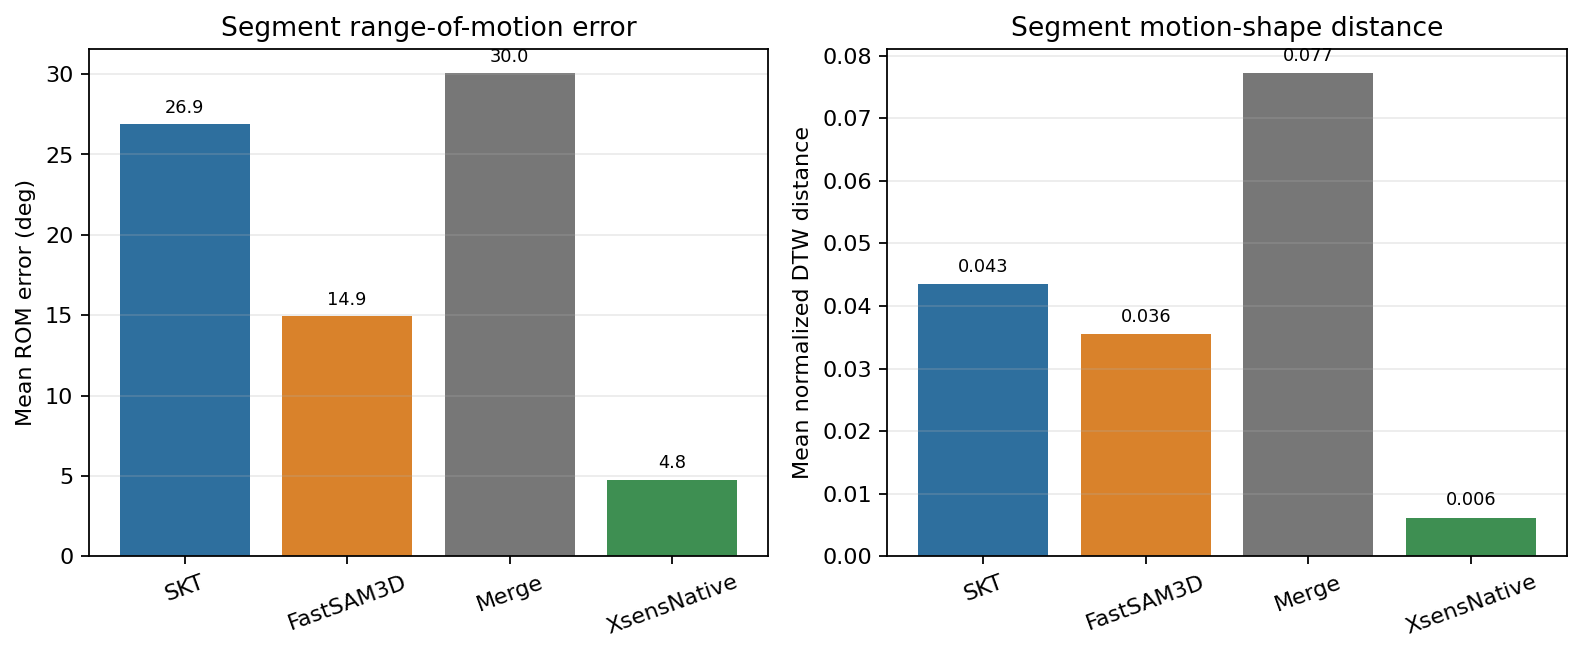
\includegraphics[width=0.95\linewidth]{thesis_segment_summary.png}
  \caption{Segment-level ROM error and DTW distance. FastSAM3D gives the strongest segment-level agreement among the vision methods, while the Xsens-native check provides a reference-system lower bound.}
  \label{fig:segment_summary_plot}
\end{figure}

\subsection{Position-space Results}

The position-space track produces a deliberately different interpretation
from the angle and motion tracks, and reading it as a competing
quality ranking would be a mistake.
SKT recovers 3D coordinates with metric scale inherited from calibrated
stereo geometry, so its distance to the Xsens-derived reference -- 30.6\,cm
mean (20.8\,cm median) after rigid Kabsch alignment -- is a meaningful
geometric quantity whose magnitude can be discussed in the same units as
the workspace itself.
FastSAM3D's direct distance to the Xsens reference under identical
coordinate assumptions is approximately 300\,cm, which is two orders of
magnitude larger; this number, however, does not say that FastSAM3D's
poses are visually two orders of magnitude worse -- it says that the raw
FastSAM3D output uses a different coordinate origin and scale convention,
and the dominant component of the 300\,cm distance is therefore a global
similarity transform that has not yet been resolved.
When FastSAM3D is instead aligned directly to SKT over a set of common
joints, the residual mean distance drops to approximately 60\,cm,
clarifying that the genuine inter-method 3D disagreement is at the
half-metre scale rather than the multi-metre scale and isolating it from
the coordinate-convention issue.

The methodological consequence is reported in
Table~\ref{tab:position_summary} rather than asserted in prose: the
position-space numbers must be read as \emph{coordinate/scale
diagnostics} that document the operational cost of using each method in
metric 3D space, not as another lap of the angle-space ranking
competition.
SKT inherits its metric scale automatically from the calibrated camera
baseline (Section~\ref{sec:data_setup}), so a downstream RULA scorer or
workspace-overlay tool can read its 3D coordinates directly; FastSAM3D
needs a separate scale/coordinate alignment step, which is feasible but
adds operational complexity that this thesis flags explicitly rather
than leaves implicit.

\begin{table}[!htbp]
  \centering
  \caption{Position-space diagnostic results. These values should be interpreted as coordinate/scale diagnostics rather than pure pose-quality rankings.}
  \label{tab:position_summary}
  \small
  \begin{tabularx}{\linewidth}{lccX}
    \toprule
    Comparison & Mean distance & Median distance & Notes \\
    \midrule
    SKT vs.\ reference & 30.6 cm & 20.8 cm & Metric stereo scale after rigid alignment \\
    FastSAM3D vs.\ reference & 300.3 cm & 294.8 cm & Coordinate/scale convention mismatch dominates \\
    FastSAM3D aligned to SKT & 60.0 cm & 36.3 cm & Direct inter-method skeleton comparison \\
    \bottomrule
  \end{tabularx}
\end{table}

\begin{figure}[!htbp]
  \centering
  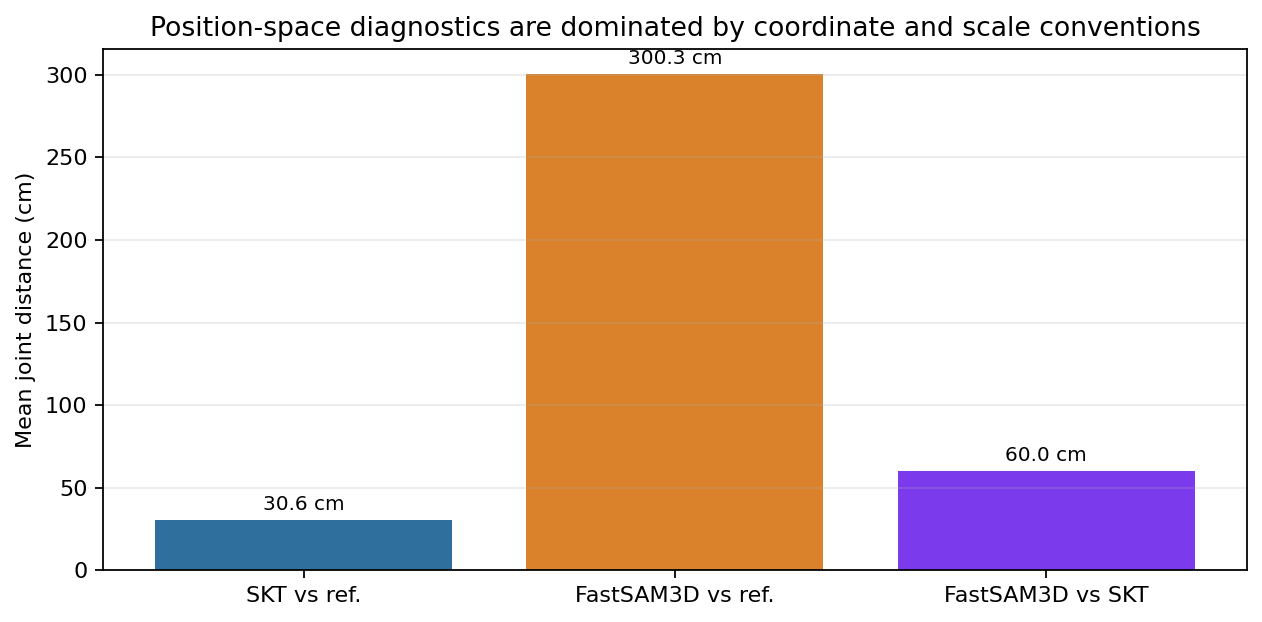
\includegraphics[width=0.9\linewidth]{thesis_position_diagnostic.png}
  \caption{Position-space diagnostic comparison. SKT is more meaningful in metric 3D space because it is tied to calibrated stereo geometry, whereas direct FastSAM3D-to-reference distance is dominated by coordinate and scale conventions.}
  \label{fig:position_diagnostic_plot}
\end{figure}

\subsection{Cross-method Synthesis}

Reading the two evaluation tracks together produces a more complete picture
than either gives on its own.
Table~\ref{tab:cross_method_synthesis} consolidates the headline numbers
for SKT and FastSAM3D (with the Xsens-native check shown alongside as a
reference-system floor).
FastSAM3D leads on the angle-space (lower MAE) and motion-space (higher
correlation) tracks, which together indicate that learned body and motion
priors suppress the per-frame jitter that hurts a frame-independent
sparse stereo reconstruction on this dataset.
SKT lags FastSAM3D on angle and motion but its 3D coordinates carry metric
scale by construction, and the per-frame geometric quality signals it exposes
(epipolar error, reprojection error, triangulation confidence) are exactly
the signals that downstream ergonomic quality gating requires.

\begin{table}[!htbp]
  \centering
  \caption{SKT vs FastSAM3D headline synthesis across evaluation tracks. Best value per column is highlighted; the Xsens-native row is a reference-system internal check, not a competing method.}
  \label{tab:cross_method_synthesis}
  \small
  \begin{tabular}{lccccl}
    \toprule
    Method & Angle MAE (\degr) $\downarrow$ & RULA bin agree.\ $\uparrow$ & Motion $r$ K=6 $\uparrow$ & Segment ROM (\degr) $\downarrow$ & Metric scale \\
    \midrule
    SKT
    & 17.6 & 0.540 & 0.379 & 26.9 & \good{Calibrated} \\
    \good{FastSAM3D}
    & \good{15.4} & \good{0.553} & \good{0.644} & \good{14.9} & Needs alignment \\
    \textit{Xsens native (ref.)}
    & \textit{4.7} & \textit{0.886} & \textit{0.965} & \textit{4.8} & \textit{---} \\
    \bottomrule
  \end{tabular}
\end{table}

The overall pattern is: \emph{the learning-based monocular pipeline wins
the angle and motion agreement tracks; the calibrated stereo pipeline
retains the deployment-geometry advantage; and neither replaces the other.}
This split is the substantive result of the synthesis and is what
Section~\ref{sec:discussion} examines in operational terms.

\clearpage
% =============================================================
\section{Discussion}
\label{sec:discussion}
% =============================================================

\subsection{Why FastSAM3D Performs Better in Angle and Motion Space}

The most likely reason FastSAM3D leads SKT on the angle and motion tracks
is that its learned body-structure and motion-continuity priors mask
exactly the per-frame failure mode that hurts a frame-independent
triangulation pipeline.
FastSAM3D's 3D output for any given frame is conditioned on body-shape
plausibility constraints that were absorbed from large pose-sequence
training corpora, so a momentarily unreliable keypoint produces a
smoothed-out anatomical correction rather than a sharp angle spike; this
is qualitatively visible in the K=6 elbow scatter plots
(Figure~\ref{fig:k6_elbow_scatter}), where the FastSAM3D scatter sits
along the ideal y=x diagonal whereas the SKT scatter shows recurring
vertical accumulation -- large target deltas at small reference deltas --
that no amount of point-density change can hide.
This shape of error matters for the interpretation: the SKT weakness is
not a uniform random noise floor but a structured failure pattern
concentrated on a small fraction of frames, which suggests that targeted
quality-aware repair rather than uniform smoothing is the appropriate
remedy.

\subsection{Why Stereo Geometry Still Matters}

The FastSAM3D advantage on the agreement tracks does not eliminate the
case for calibrated stereo geometry, because deployment in a real
manufacturing setting cares about two properties that the agreement
tracks alone do not test: whether the 3D coordinates are in real metric
units, and whether the system can flag its own unreliable frames before
they reach a downstream ergonomic risk score.
SKT inherits metric scale from the calibrated camera baseline, so its 3D
coordinates can be overlaid on workspace geometry without an additional
alignment step, whereas any monocular learning-based pipeline needs an
explicit external scale and coordinate recovery before its output is
usable in the same role.
More importantly, SKT exposes a per-frame geometric quality vector --
triangulation confidence, epipolar error, reprojection error,
left--right keypoint agreement -- whose individual components are tied
to the camera model, so an automated downstream stage can refuse to
score frames whose quality vector falls outside the working envelope;
an end-to-end learned pipeline can in principle be augmented with
calibrated uncertainty heads, but that augmentation is itself an open
research problem rather than a property the FastSAM3D output exposes
today.

\subsection{Failure-case Analysis of High-delta Events}

The K=6 scatter pattern noted above is not generic noise but a small
number of identifiable keypoint-chain failures, and treating it as
such is what makes the next SKT iteration tractable.
For elbow flexion, the relevant chain is shoulder--elbow--wrist; an
unstable wrist detection in either camera can leave the triangulated
shoulder and elbow correct, satisfy all geometric quality checks
individually, and still produce an elbow angle that jumps by tens of
degrees in a single frame, because the angle depends on the relative
direction of two segments rather than on the absolute position of any
single keypoint.
Figure~\ref{fig:skt_high_delta_cases} shows two representative SKT
high-delta intervals projected back onto the original video; the
problematic frames in each clip share three concrete characteristics --
partial occlusion of the wrist by the body or by an object, large
camera-to-subject distance, and inconsistent left/right detection of
the elbow chain -- rather than appearing at random across the
recording.
The operational implication is that the next SKT improvement should
focus on chain-aware (not single-keypoint-aware) quality filtering
together with short-window temporal repair, since both interventions
target the specific failure mode evidenced here and neither requires
changing the underlying triangulation or angle formula.

\subsection{Applicability Boundaries}

Putting these analyses together gives a concrete recommendation for
when each method type should be preferred in industrial ergonomic
monitoring, rather than a universal ranking statement.
For deployment scenarios that need only joint-angle outputs and short-term
motion signals -- for example a fixed-camera workstation that scores
postures from skeletons but does not need to overlay them on real
geometry -- a learning-based monocular pipeline of the FastSAM3D family
is the more competitive choice on this dataset, both because its
absolute angle MAE is lower and because its short-term motion signal is
visibly more stable.
For deployment scenarios that need metric 3D scale, workspace overlay,
or per-frame quality gating before downstream automated scoring -- which
is the more typical industrial setting -- calibrated stereo remains
the more defensible default, because both the metric coordinates and
the geometric quality signals are properties of the camera model rather
than of the trained model.
The thesis therefore does not recommend one method as universally
correct, and the practical question for any new deployment is which of
these two sets of requirements dominates.

\begin{figure}[!htbp]
  \centering
  \begin{subfigure}[b]{0.98\linewidth}
    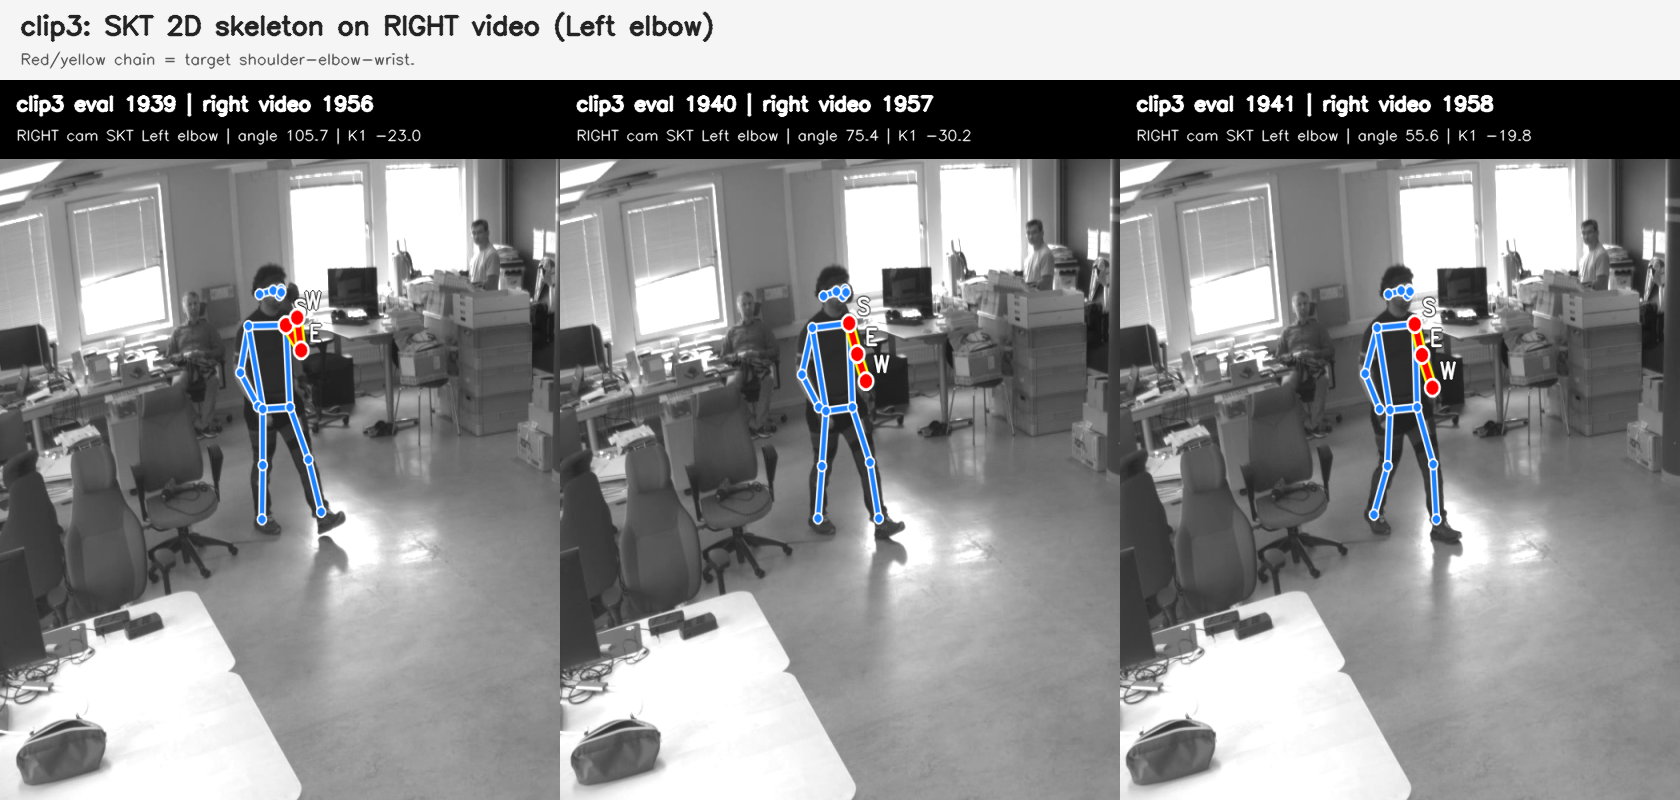
\includegraphics[width=\linewidth]{thesis_skt_high_delta_left_elbow_frames.png}
    \caption{Left-elbow high-delta interval.}
  \end{subfigure}

  \vspace{0.35cm}
  \begin{subfigure}[b]{0.98\linewidth}
    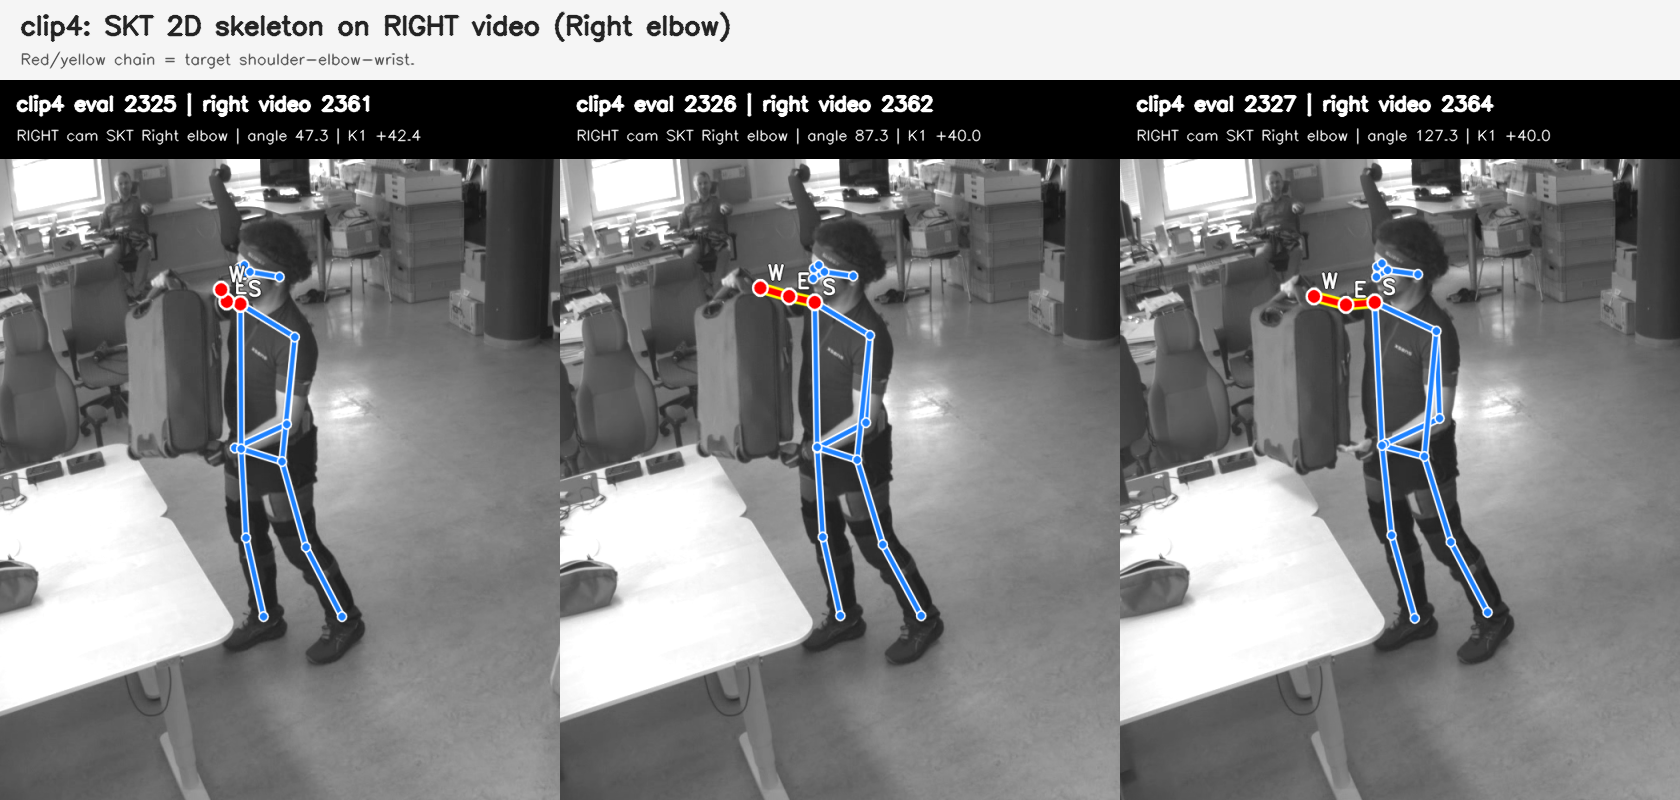
\includegraphics[width=\linewidth]{thesis_skt_high_delta_right_elbow_frames.png}
    \caption{Right-elbow high-delta interval.}
  \end{subfigure}
  \caption{Representative SKT high-delta diagnostic frames projected onto the original video view. These examples indicate that some large motion deltas are caused by local keypoint instability around the elbow chain rather than by physically implausible whole-body motion.}
  \label{fig:skt_high_delta_cases}
\end{figure}

\subsection{Limitations}

Four limitations of the present study set the boundary inside which all
quantitative results above should be read; they are stated explicitly here
so that the conclusion in Section~\ref{sec:conclusion} can rest on
honestly scoped evidence rather than on an over-generalised claim.
\emph{First}, all results come from a single subject performing a single
controlled recording in a manufacturing-like environment; the
between-method ranking should therefore be read as supported on this
dataset rather than as a general statement about every operator,
clothing style, lighting condition, or camera distance.
\emph{Second}, the deepest motion-space analysis focuses on the elbow,
which is the joint that the project investigated most carefully and the
joint whose Xsens calibration limitation is best quantified; the
motion-space numbers for the shoulder, hip, and knee are reported but
should be read with weaker confidence than the elbow numbers because
their reference floor is less well characterised.
\emph{Third}, the evaluation outputs depend on the smoothing window, the
segment-detection thresholds, and the constant-offset assumption used for
time alignment; the pipeline records these settings explicitly in the run
configuration so that any future work can rerun the same comparison under
different choices, and the synchronisation analysis in
Section~\ref{sec:data_setup} shows that the constant-offset assumption is
adequate for this recording but does not prove it for longer recordings.
\emph{Fourth}, Xsens is used throughout as an external comparison
reference and not as physical ground truth; the absolute angle errors are
therefore interpreted alongside the Xsens self-consistency floor
established in Section~\ref{sec:data_setup} rather than as direct error
against a true biomechanical zero.

\subsection{Implications for Real-time Deployment}

The deployment path that follows most cleanly from the above is to
prioritise getting the calibrated SKT pipeline running efficiently on
GPU hardware before treating learning-based pose models as
replacements rather than as optional stabilisers.
The concrete engineering steps are well-established: export the 2D pose
model to TensorRT, move video decoding and preprocessing onto the GPU,
and keep triangulation and joint-angle computation lightweight enough to
remain in the streaming budget; lightweight real-time pose models such
as RTMPose \cite{jiang2023rtmpose} make this direction realistic at the
2D-detection stage, although the final reportable number must be
end-to-end latency rather than model inference time alone, because
decoding, preprocessing, and post-processing each consume a measurable
share of the per-frame budget.
Once this baseline streams reliably, the two natural extensions are
(i) integrating a learning-based pose head -- of the FastSAM3D family --
as an optional smoothing or fallback signal when SKT quality flags drop
below an acceptable threshold, and (ii) introducing transformer-based
temporal priors to repair the keypoint-chain failures identified in the
high-delta analysis above; both extensions are framed here as
\emph{stabilisers on top of} the calibrated stereo baseline rather than
as replacements for it, because the deployment-geometry advantages
discussed in Section~7.2 do not transfer to a pure monocular pipeline
without additional scale/coordinate work.

\clearpage
% =============================================================
\section{Conclusion and Future Work}
\label{sec:conclusion}
% =============================================================

\subsection{Conclusion}

This thesis evaluates 3D human pose estimation for manufacturing-oriented
ergonomic monitoring using a three-axis framework -- angle-space,
motion-space, and position-space -- against an Xsens reference whose
calibration limitation is explicitly quantified rather than ignored.
On the single-subject manufacturing recording used here, the
learning-based monocular FastSAM3D pipeline delivers better
agreement-track numbers (mean angle MAE 15.4\degr\ vs.\ 17.6\degr; mean
K=6 motion Pearson 0.64 vs.\ 0.38; segment ROM error 14.9\degr\ vs.\
26.9\degr) than the calibrated stereo SKT pipeline.
SKT nevertheless retains the only metric-scale 3D output among the
evaluated pipelines and is the only pipeline that exposes per-frame
geometric quality signals usable for downstream quality gating, so it
remains the right choice when deployment requires real units or
self-reported reliability rather than only joint-angle smoothness.
The substantive conclusion is therefore not a single recommended method
but a deliberate split: learning-based monocular pose is competitive
when the deployment task is restricted to joint angles and short-term
motion, while calibrated stereo is necessary when the deployment task
extends to metric 3D scale and explainable per-frame quality, and a
future ergonomic monitoring system is likely to want both -- learned
priors for body-pose stability, stereo geometry for scale and
deployment transparency.

\subsection{Future Work}

Three follow-up directions are required before the present results can
be claimed as generally applicable rather than as evidence for a single
controlled recording.

\begin{enumerate}[leftmargin=1.2cm]
  \item \textbf{Validation on additional recordings and subjects.}
        Repeat the same three-axis protocol on at least one additional
        operator, additional clothing, additional lighting, and an
        unscripted task, in order to test whether the FastSAM3D
        agreement-track advantage generalises and whether the SKT
        high-delta failure modes recur in the same shoulder--elbow--wrist
        chain across subjects.
  \item \textbf{Real-time GPU deployment of SKT with optional learned
        stabilisers.} Move the SKT 2D backbone to TensorRT and the
        decoding/preprocessing onto the GPU, measure end-to-end streaming
        latency rather than model inference time alone, and then evaluate
        a FastSAM3D-style learned head as an optional smoothing or
        fallback signal triggered when SKT quality flags drop below the
        deployment threshold.
  \item \textbf{Beyond-elbow motion analysis and connection to a complete
        ergonomic risk score.} Extend the motion-space analysis to the
        shoulder, hip, and knee with the same reference-floor
        quantification that this thesis applies to the elbow, and then
        connect the resulting joint-angle stream to a full ergonomic
        risk score (e.g.\ RULA, REBA) rather than to RULA-bin agreement
        alone, so that pose-estimation quality and downstream
        risk-classification quality can be reported as a single
        deployment-relevant pipeline.
\end{enumerate}

\subsection{Recommended Next-stage Experimental Protocol}

To make the validation-on-new-datasets step above repeatable rather than
ad hoc, this subsection consolidates the working protocol used in the
present recording into a five-stage checklist
(Table~\ref{tab:validation_checklist}) that future datasets should run
\emph{in order}, with each stage gating the next.
The protocol enforces two methodological principles that emerged from
the present study.
The first principle is that data-ingestion integrity (orientation,
frame-ID re-pairing, timestamp monotonicity, calibration compatibility)
must be verified before any accuracy number is computed, because the
most expensive class of failure in the present pipeline is
mis-interpreting an ingestion bug as a pose-estimation result.
The second principle is that algorithmic changes and protocol changes
must be evaluated separately: if SKT is later modified with stronger
2D-keypoint filtering or a temporal repair module, the same K-frame
motion-delta protocol must be rerun before and after the modification
so that the comparison is fair, and if a new learning-based method is
added, its coordinate convention and filtering state must be recorded
before it is included in the position-space analysis.

\begin{table}[!htbp]
  \centering
  \caption{Five-stage validation checklist for extending the present thesis evaluation to new manufacturing recordings. Stages should be executed in order; each stage gates the next.}
  \label{tab:validation_checklist}
  \small
  \begin{tabularx}{\linewidth}{p{3.2cm}XX}
    \toprule
    Stage & What should be checked & Why it matters \\
    \midrule
    Dataset validation
    & Video orientation, hardware frame IDs, metadata timestamps, synchronised frame count, and camera calibration compatibility.
    & Prevents data-ingestion errors from being mis-interpreted as pose-estimation errors. \\
    Time alignment
    & Automatic offset curves on three independent scores, residual lag at the beginning and end of the recording, and common valid intervals.
    & Ensures that motion-space metrics compare the same physical movement period. \\
    Method comparison
    & Angle MAE, K-frame motion agreement at $K\in\{1,6,12,25\}$, segment ROM and DTW, and position-space diagnostics for every method.
    & Keeps the comparison multi-dimensional and avoids over-ranking methods by a single metric. \\
    Failure analysis
    & High-delta frames, occlusion cases, camera distance, and left--right keypoint consistency.
    & Connects quantitative outliers to concrete visual causes and guides targeted SKT repair work. \\
    Deployment check
    & End-to-end streaming latency, GPU preprocessing, model inference time, and stability under streaming input.
    & Tests whether the method can move from offline evaluation toward real-time ergonomic monitoring. \\
    \bottomrule
  \end{tabularx}
\end{table}

The final thesis version should therefore deliver two distinct kinds of
evidence rather than a single aggregate error number.
The first is \emph{quantitative agreement} across several recordings and
movement types, run through the checklist above so that the comparison
remains multi-dimensional and protocol-controlled.
The second is \emph{diagnostic evidence} that exposes when and why each
pipeline fails and which subsystem is responsible, of the kind that
Section~\ref{sec:discussion} presented for the SKT high-delta cases.
This combination is the right level of evidence for ergonomic deployment
in manufacturing, because a practical monitoring system needs not only
to be accurate on average but also to know -- and to expose -- when its
output should not be trusted.

\clearpage
% =============================================================
\appendix
\clearpage
% =============================================================

\section{Stereo Calibration Parameters}
\label{app:calibration}

The numerical calibration values reported below are the optimised parameters
that all SKT experiments in the thesis use as fixed input; the
binary form is stored at \texttt{shared/camera\_params.npz} and is loaded
directly by the pose pipeline.
The intrinsic matrices follow the OpenCV convention $K = [[f_x, 0, c_x];
[0, f_y, c_y]; [0,0,1]]$ in pixels, the distortion vectors follow the
14-parameter rational model used by OpenCV's \texttt{cv2.calibrateCamera}
(only the first 8 entries are non-zero in this calibration), and the
stereo extrinsics give the rotation $R$ and translation $T$ that map a
3D point from the left to the right camera frame in centimetres.

\begin{table}[!htbp]
  \centering
  \caption{Left and right camera intrinsic matrices (pixels) and the stereo extrinsic baseline.}
  \label{tab:calib_intrinsics}
  \small
  \begin{tabular}{lcc}
    \toprule
    Quantity & Left camera & Right camera \\
    \midrule
    $f_x$ (pixels)            & 1130.27 & 1129.01 \\
    $f_y$ (pixels)            & 1130.35 & 1129.63 \\
    $c_x$ (pixels)            & 1019.32 & 1028.31 \\
    $c_y$ (pixels)            &  825.72 &  826.35 \\
    \midrule
    Stereo baseline $\|T\|$   & \multicolumn{2}{c}{41.27\,cm} \\
    Image resolution          & \multicolumn{2}{c}{2048 $\times$ 1536} \\
    Distortion model          & \multicolumn{2}{c}{OpenCV rational (14-parameter)} \\
    \bottomrule
  \end{tabular}
\end{table}

The stereo rotation $R$ deviates from the identity by less than 0.011
radians on each off-diagonal entry, consistent with a near-aligned
parallel-baseline rig, and the translation vector
$T \approx [-41.27, -0.03, 0.04]^T$\,cm confirms that the baseline is
dominated by the $x$ axis as designed.
The essential matrix $E$ and fundamental matrix $F$ recorded in
\texttt{camera\_params.npz} are derived from $R$ and $T$ together with
the two intrinsic matrices and are not duplicated here.
The full distortion coefficients and the original calibration session
metadata (target type, number of valid views, per-view reprojection
residuals) are stored alongside the matrices in the same NPZ file.

\FloatBarrier
\clearpage
\section{Sensitivity Analyses}
\label{app:sensitivity}

The headline numbers reported in Section~\ref{sec:results} depend on
three parameter choices made in the evaluation pipeline: the camera-side
smoothing window, the activity-segment detection threshold, and the
DTW preprocessing convention.
This appendix reports how the SKT motion and segment-level numbers move
when each choice is varied, so that the reader can judge how brittle the
conclusion is.

\begin{table}[!htbp]
  \centering
  \caption{Sensitivity of SKT motion-space and segment-level numbers to the camera-side moving-average smoothing window, on the present recording. The 200\,ms and 300\,ms rows are identical because both round to a 3-frame centred window at 12.5\,fps.}
  \label{tab:sens_smoothing}
  \footnotesize
  \setlength{\tabcolsep}{4pt}
  \resizebox{\linewidth}{!}{%
  \begin{tabular}{lcccc}
    \toprule
    Window & Frames & SKT K=6 Pearson (L/R) & SKT ROM MAE (L/R, \degr) & K=1 quiet std (L/R, \degr) \\
    \midrule
    100\,ms & 1 & -- / --   & 38.4 / 33.3 & --   / --   \\
    200\,ms & 3 & 0.41 / 0.40 & 19.3 / 21.3 & 7.0 / 6.6 \\
    300\,ms & 3 & 0.41 / 0.40 & 19.3 / 21.3 & 7.0 / 6.6 \\
    400\,ms & 5 & 0.43 / 0.42 & 16.4 / 21.8 & 4.4 / 4.5 \\
    \bottomrule
  \end{tabular}%
  }
\end{table}

The 200\,ms working point chosen in the main body is the
literature-supported rule of thumb for non-explosive human motion; a
400\,ms window further reduces SKT quiet-frame jitter below the
$<$5\degr/frame validation target at the cost of a slightly weaker
short-term motion signal, and is reported here as the
``conservative-smoothing'' alternative for future runs.

\begin{table}[!htbp]
  \centering
  \caption{Sensitivity of detected segment counts to the activity-detection threshold (applied to the Xsens-derived reference K-frame deltas).}
  \label{tab:sens_segments}
  \small
  \begin{tabular}{lcc}
    \toprule
    Activity threshold (\degr) & Left-elbow segments & Right-elbow segments \\
    \midrule
    8  & 5  & 7  \\
    10 (default) & 8 & 9 \\
    12 & 13 & 15 \\
    \bottomrule
  \end{tabular}
\end{table}

Segment counts vary by a factor of roughly 2--3 across the tested
threshold range, but the cross-method ranking inside each row is stable:
FastSAM3D maintains the lowest segment ROM MAE and DTW distance
regardless of the threshold setting, so the main-body conclusion does
not depend on the specific threshold value chosen.
The DTW preprocessing sweep (\texttt{mean\_l2}, \texttt{mean}, and
\texttt{none}) confirms that the mean-subtracted, L2-normalised
convention adopted in the main body is the version under which the
XsensNative-vs-XsensFair anchor DTW remains near zero; without L2
normalisation the DTW distance becomes dominated by amplitude rather
than by shape, which is the explicit motivation for the chosen
preprocessing.

\FloatBarrier
\clearpage
\section{Implementation and Reproducibility Notes}
\label{app:repro}

The standalone evaluation workflow is implemented in
\texttt{00\_pose\_pipeline/}.
For the present dataset, the main reproduction command is:
\begin{footnotesize}
\begin{verbatim}
/opt/anaconda3/envs/pose/bin/python \
  00_pose_pipeline/src/run_pipeline.py \
  --config \
  00_pose_pipeline/configs/current_2025_ergonomics.yaml \
  --stages \
  validate,offset,angle,motion,segment,scatter
\end{verbatim}
\end{footnotesize}

The configuration file records the dataset-specific choices that
otherwise must be inferred from prose alone: the 180\degr\ video
rotation, the hardware-frame-ID synchronisation rule, the metadata
timestamp-parsing convention, the calibration NPZ path, the per-system
smoothing settings, the K-frame list $\{1,6,12,25\}$, the
activity-detection threshold, and the automatic offset-search range.
Generated outputs are stored under \texttt{00\_pose\_pipeline/runs/}
and include both the headline tables/figures referenced from the main
body and the per-stage diagnostics that drive Section~\ref{sec:discussion}.

Figure~\ref{fig:residual_lag_check} reports a residual lag diagnostic
that the pipeline can produce after the selected constant offset has
been applied; it is not a headline result but it documents the
sanity-check evidence used to defend the constant-offset assumption in
Section~\ref{sec:data_setup}.

\begin{figure}[!htbp]
  \centering
  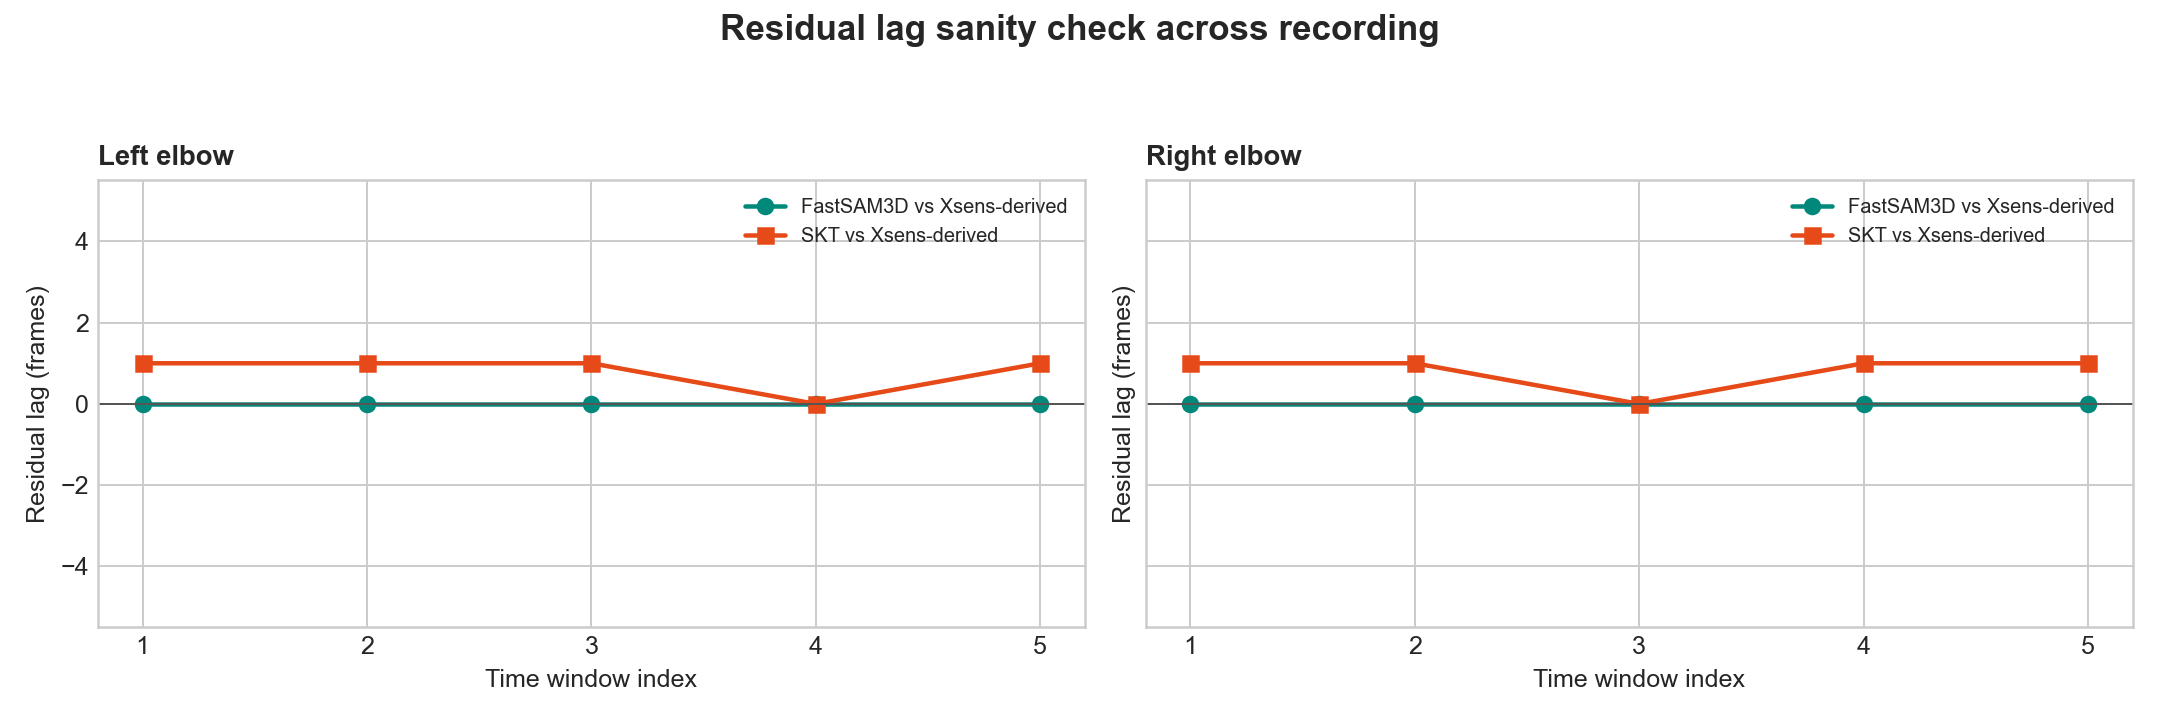
\includegraphics[width=\linewidth]{thesis_residual_lag_drift_check.png}
  \caption{Residual lag sanity check after applying the selected constant offset. The figure supports the assumption that a constant offset is adequate for the present recording, while explicitly acknowledging that future longer or multi-take recordings should rerun this check.}
  \label{fig:residual_lag_check}
\end{figure}

\FloatBarrier
\clearpage
\section{Claim-evidence Self-review}
\label{app:claim_evidence}

The table below maps every major thesis claim back to its supporting
evidence in this draft, following the
``Claim $|$ Evidence $|$ Status'' convention recommended for
adversarial paper review.
Claims marked \emph{Needs evidence} are stated as open items rather
than as supported conclusions, and the conclusion in
Section~\ref{sec:conclusion} is restricted to the claims marked
\emph{Supported}.

\begin{table}[H]
  \centering
  \caption{Claim-evidence map for the present thesis draft.}
  \label{tab:claim_evidence}
  \small
  \renewcommand{\arraystretch}{1.12}
  \begin{tabularx}{\linewidth}{p{4.0cm}Xp{1.9cm}}
    \toprule
    Claim & Evidence used in this draft & Status \\
    \midrule
    FastSAM3D is stronger than SKT in angle-space on the present dataset.
    & Table~\ref{tab:angle_summary} and Figure~\ref{fig:angle_summary_plot}: 15.4\degr\ mean MAE vs.\ 17.6\degr.
    & Supported \\
    FastSAM3D is stronger than SKT in K=6 motion-space agreement.
    & Table~\ref{tab:motion_summary}, Figure~\ref{fig:motion_k6_summary_plot}, and Figure~\ref{fig:k6_elbow_scatter}: mean Pearson 0.644 vs.\ 0.379; elbow correlations 0.54/0.69 vs.\ 0.39/0.39.
    & Supported \\
    SKT retains a position-space and interpretability advantage.
    & Table~\ref{tab:position_summary}, Figure~\ref{fig:position_diagnostic_plot}, and the SKT method design; SKT uses calibrated stereo scale and exposes per-frame geometric quality signals.
    & Supported \\
    A constant cross-system offset is adequate for the current recording.
    & Figure~\ref{fig:offset_search}, Figure~\ref{fig:first_last_delta}, and Figure~\ref{fig:residual_lag_check}; the three independent offset scores converge within $\sim$0.04\,s.
    & Supported for present recording \\
    SKT high-delta points are caused by local keypoint-chain instability.
    & Figure~\ref{fig:skt_high_delta_cases}: diagnostic frames show partial wrist occlusion, large camera distance, and inconsistent left/right elbow-chain detection during the high-delta intervals.
    & Supported qualitatively \\
    The SKT vs FastSAM3D ranking is robust to smoothing and segmentation parameters.
    & Appendix~\ref{app:sensitivity}: sensitivity tables across smoothing windows and activity thresholds preserve the FastSAM3D $>$ SKT ranking.
    & Supported \\
    Results generalise to manufacturing environments broadly.
    & Only one controlled single-subject dataset is evaluated.
    & Needs evidence \\
    Full RULA automation is solved.
    & Only continuous angle MAE and RULA-like bin agreement are reported; RULA scoring requires additional load/twist/repetition information.
    & Not claimed \\
    \bottomrule
  \end{tabularx}
\end{table}

\clearpage

\begin{thebibliography}{99}

\bibitem{mcatamney1993rula}
L.~McAtamney and E.~N.~Corlett,
\textit{RULA: a survey method for the investigation of work-related upper limb disorders},
Applied Ergonomics, vol.~24, no.~2, pp.~91--99, 1993.

\bibitem{menolotto2020motion}
M.~Menolotto, D.-S.~Komaris, S.~Tedesco, B.~O'Flynn, and M.~Walsh,
\textit{Motion capture technology in industrial applications: A systematic review},
Sensors, vol.~20, no.~19, article 5687, 2020.

\bibitem{yu2019joint}
Y.~Yu, X.~Yang, H.~Li, X.~Luo, and H.~Guo,
\textit{Joint-level vision-based ergonomic assessment tool for construction workers},
Journal of Construction Engineering and Management, vol.~145, no.~5, 2019.

\bibitem{menanno2024ergonomic}
M.~Menanno, C.~Riccio, V.~Benedetto, and G.~Palmieri,
\textit{An ergonomic risk assessment system based on 3D human pose estimation and collaborative robot},
Applied Sciences, vol.~14, no.~11, article 4823, 2024.

\bibitem{quesada2026supporting}
A.~Quesada Diaz, A.~Iriondo Pascual, L.~Hanson, D.~H{\"o}gberg, and A.~Syberfeldt,
\textit{Supporting ergonomics evaluations in manufacturing: A comparison of computer vision- and IMU-based motion capture},
IOP Conference Series: Materials Science and Engineering, vol.~1342, article 012053, 2026.

\bibitem{iriondo2024development}
A.~Iriondo Pascual, L.~Hanson, D.~H{\"o}gberg, E.~Brolin, and A.~Syberfeldt,
\textit{Development and initial usability evaluation of a digital tool for simulation-based multi-objective optimization of productivity and worker well-being},
Advanced Engineering Informatics, vol.~60, article 102726, 2024.

\bibitem{iriondo2025integrating}
A.~Iriondo Pascual, L.~Hanson, E.~Brolin, D.~H{\"o}gberg, and A.~Syberfeldt,
\textit{Integrating motion capture and digital human modelling tools for worker ergonomics assessment: A case study from experimental lab to real-world manufacturing},
Lecture Notes in Computer Science, vol.~15828, pp.~324--333, 2025.

\bibitem{filippeschi2017survey}
A.~Filippeschi, N.~Schmitz, M.~Miezal, G.~Bleser, E.~Ruffaldi, and D.~Stricker,
\textit{Survey of motion tracking methods based on inertial sensors: A focus on upper limb human motion},
Sensors, vol.~17, no.~6, article 1257, 2017.

\bibitem{roetenberg2009xsens}
D.~Roetenberg, H.~Luinge, and P.~Slycke,
\textit{Xsens MVN: Full 6DOF human motion tracking using miniature inertial sensors},
Xsens Technologies technical report, 2009.

\bibitem{cao2019openpose}
Z.~Cao, G.~Hidalgo, T.~Simon, S.-E.~Wei, and Y.~Sheikh,
\textit{OpenPose: Realtime multi-person 2D pose estimation using part affinity fields},
IEEE Transactions on Pattern Analysis and Machine Intelligence,
vol.~43, no.~1, pp.~172--186, 2019.

\bibitem{jiang2023rtmpose}
T.~Jiang, P.~Lu, L.~Zhang, N.~Ma, R.~Han, C.~Lyu, Y.~Li, and K.~Chen,
\textit{RTMPose: Real-time multi-person pose estimation based on MMPose},
arXiv preprint arXiv:2303.07399, 2023.

\bibitem{pavllo20193d}
D.~Pavllo, C.~Feichtenhofer, D.~Grangier, and M.~Auli,
\textit{3D human pose estimation in video with temporal convolutions and semi-supervised training},
Proceedings of the IEEE/CVF Conference on Computer Vision and Pattern Recognition, pp.~7753--7762, 2019.

\bibitem{zhu2023motionbert}
W.~Zhu, X.~Ma, Z.~Liu, L.~Liu, W.~Wu, and Y.~Wang,
\textit{MotionBERT: A unified perspective on learning human motion representation},
Proceedings of the IEEE/CVF International Conference on Computer Vision, pp.~15085--15099, 2023.

\bibitem{yang2026fastsam3d}
T.~Yang, S.~He, H.~Jing, J.~Yang, Z.~Liu, C.~Zou, and Y.~Wang,
\textit{Fast SAM 3D Body: Accelerating SAM 3D Body for Real-Time Full-Body Human Mesh Recovery},
arXiv preprint arXiv:2603.15603, 2026.

\bibitem{hartley2004multiple}
R.~Hartley and A.~Zisserman,
\textit{Multiple View Geometry in Computer Vision},
2nd ed., Cambridge University Press, 2004.

\bibitem{hirschmuller2007sgbm}
H.~Hirschm{\"u}ller,
\textit{Stereo processing by semiglobal matching and mutual information},
IEEE Transactions on Pattern Analysis and Machine Intelligence,
vol.~30, no.~2, pp.~328--341, 2007.

\bibitem{kabsch1976solution}
W.~Kabsch,
\textit{A solution for the best rotation to relate two sets of vectors},
Acta Crystallographica, Section A, vol.~32, pp.~922--923, 1976.

\bibitem{sakoe1978dtw}
H.~Sakoe and S.~Chiba,
\textit{Dynamic programming algorithm optimization for spoken word recognition},
IEEE Transactions on Acoustics, Speech, and Signal Processing,
vol.~26, no.~1, pp.~43--49, 1978.

\bibitem{perezluque2026reaching}
E.~P{\'e}rez Luque, S.~Lee, D.~H{\"o}gberg, J.~Yang, and M.~Lamb,
\textit{Predicting human upper extremity reaching motions: Comparison of optimization-based method and heuristic method},
International Journal of Human--Computer Interaction, 2026.
DOI: 10.1080/10447318.2026.2632154.

\end{thebibliography}

\end{document}
